\documentclass[11pt]{article}

\usepackage[T1]{fontenc}
\usepackage{lmodern}
\usepackage{microtype}
\usepackage{amsmath,amssymb,amsthm,mathtools}
\numberwithin{equation}{section}
\usepackage{enumitem}
\usepackage{array}
\usepackage{tabularx}
\usepackage{geometry}
\geometry{margin=1in}
\usepackage{cite}
\usepackage{hyperref}
\usepackage{url}
\usepackage{tikz}
\usepackage{longtable}
\hypersetup{hidelinks}
\setlength{\emergencystretch}{3em}
\clubpenalty=5000
\widowpenalty=5000
\displaywidowpenalty=5000

\theoremstyle{plain}
\newtheorem{theorem}{Theorem}[section]
\newtheorem{lemma}[theorem]{Lemma}
\newtheorem{proposition}[theorem]{Proposition}
\newtheorem{corollary}[theorem]{Corollary}
\theoremstyle{definition}
\newtheorem{definition}[theorem]{Definition}
\theoremstyle{remark}
\newtheorem{remark}[theorem]{Remark}
\newtheorem{example}[theorem]{Example}
\newtheorem{openproblem}[theorem]{Open Problem}
\newtheorem{conjecture}[theorem]{Conjecture}
\newtheorem{rresult}[theorem]{Research Result}
\newtheorem{rrefuted}[theorem]{Refuted Claim}

\newcommand{\Wit}{\mathsf{W}}
\newcommand{\Cmcf}[2]{\mathcal{C}^{\mathrm{mcf}}_{#1,#2}}
\newcommand{\D}{\mathcal{D}}
\newcommand{\out}{\mathrm{out}}
\newcommand{\tuple}[1]{\vec{#1}}
\newcommand{\blank}{\square}
\newcommand{\eps}{\varepsilon}
\newcommand{\pausesym}{\bot}
\newcommand{\fan}{\operatorname{fan}}
\newcommand{\YSub}[1]{\mathsf{YSub}(#1)}
\newcommand{\YSL}[2]{\mathsf{YSL}(#1,#2)}
\newcommand{\evalmap}{\mathsf{ev}}

\newcommand{\cutpos}[1]{%
  \raisebox{-0.7ex}{%
    \tikz[baseline=(char.base)]{%
      \node[draw,circle,inner sep=0.4pt,font=\scriptsize]
        (char) {\ensuremath{#1}};%
    }%
  }%
}

\theoremstyle{plain}
\newtheorem{mainthm}{Theorem}
\renewcommand{\themainthm}{\Alph{mainthm}}
\newcommand{\provenance}[1]{\par\noindent{\small\textit{Provenance.} #1}\par\medskip}
\setcounter{tocdepth}{2}

\title{\#2 Research Compendium (02-v4-fixed-s-mcfg):\\
Multiple Context-Free Languages under Fixed Finite-Semigroup Typing\\[0.4ex]
\large All results of the v1 and v2 research lines, 2026-10 -- 2026-11}
\author{Takayuki Kuriyama\\
Independent Researcher, Tokyo, Japan\\
\texttt{growup.kuriyama@gmail.com}}
\date{Compiled 2026-11-21}

\begin{document}
\maketitle

\begin{abstract}
This compendium collects in one document every result of the author's research on
positive-data learning of multiple context-free languages under a fixed finite-semigroup
typing $s$ (the ``fixed-$s$ MCFG'' line, paper~\#2).  It merges the former folders
\texttt{02\_fixed-h-mcfg} (v1, arXiv:2605.11644) and
\texttt{02-v2-lg-fanout-boundary} (v2), which now live under \texttt{02-v4-fixed-s-mcfg/v1}
and \texttt{02-v4-fixed-s-mcfg/v2}.

Part~\ref{part:core} is the fullest version of the paper: local-group typings admit
characteristic samples of total length $O(\|G\|^2\bar\theta_G)$ at every fixed fan-out and
rank; over large alphabets every typing needs $\Omega(\|G\|\bar\theta_G)$; at fan-out one
$\mathbf{LG}$ is the exact pseudovariety boundary, typings onto $U_1$ are classified, and
isolated letters give polynomial data; at fan-out two the doubling family does not lift,
two-letter semilattice typings have polynomial data, and the boundary question reduces to
content typings.  Part~\ref{part:v2-further} adds every other proved result of v2,
Part~\ref{part:v1} the parked results of v1, and Part~\ref{part:fanout-two-research} the
research record on the fan-out-two boundary, with the verification status of each claim.
The boundary at fan-out two (Open Problem~\ref{op:fanout-two}) remains open.
\end{abstract}

\section*{Guide to This Compendium}
\addcontentsline{toc}{section}{Guide to This Compendium}

\paragraph{Purpose.}
This is a working master, not a submission.  Page count is not a constraint: every
statement that ever appeared in a v1 or v2 manuscript, a parked file, or an audited research
report is included once, in its latest version.  Submission-sized papers are cut from it;
the current derived paper is \texttt{02-v3-cfg-typing-classification} (the new paper~\#2,
fan-out one).

\paragraph{Sources and precedence.}
For a statement that exists in several versions, the latest one is used:
Plan~A \texttt{v2/main.tex} (2026-11-17) $>$ the 43-page v2 source of 2026-11-13 $>$ the
64-page v2 source of 2026-11-11 $>$ parked v2 blocks (2026-11-09, 11-06, 10-31) $>$ v1
(2026-10-31) and its parked blocks.  Every section of Parts~\ref{part:v2-further}
and~\ref{part:v1} begins with a provenance note naming its source file; the text is copied
verbatim apart from section levels, label suffixes that avoid clashes (for example
\texttt{-foc}, \texttt{-u1}, \texttt{-v1s}), and notes marked \emph{Compendium note}.

\paragraph{Status.}
Parts~\ref{part:core}--\ref{part:v1} contain statements with complete proofs written for the
manuscripts.  They have been checked repeatedly by the author and by AI models, but have
not been peer reviewed.  Part~\ref{part:fanout-two-research} contains research results; each
is labelled \emph{Research Result} or \emph{Refuted Claim} and carries its status (hand-audited,
conditional, refuted, open, certified finite) and its source in \texttt{v2/reviews/}, where
the full arguments, checkers and audits are kept.

\paragraph{Overlapping versions.}
Some results occur twice in different strength: the fan-out-one lower bound is proved both
by the three-letter family (Proposition~\ref{prop:three-letter-family}) and by the companion's
five-letter family (Subsection~\ref{subsec:light-route}); the binary typing onto $U_1$ at
fan-out two has its own proof (Section~\ref{sec:p2-binary-u1-fanout2}) besides
Corollary~\ref{cor:two-letter-semilattice}; Open Problem~S1 of 2026-11-06
(Section~\ref{sec:p2-rare-type-programme}) was later resolved by
Corollary~\ref{cor:two-letter-fanout-one}.  Such cases are marked where they occur.

\tableofcontents
\clearpage

\part{The Main Paper: Characteristic-Data Length under Fixed Finite-Semigroup Typing}
\label{part:core}

\provenance{v2 manuscript of 2026-11-13 (43 pp., \path{v2/parked/planA_2026-11-16/original_en_43pp.tex}), with the refinements of the Plan~A version (\path{v2/main.tex}, 2026-11-17) to the local-group proof chain, and with the fan-out-one $U_1$ results, the two-letter and semilattice results and Proposition~\ref{prop:zeta-capacity} of the 64-page version of 2026-11-11 (blob \texttt{d7bb4f7}), restored at their original places.  Subsection~\ref{subsec:light-route} is the Plan~A route through the companion paper.}

\section{Introduction}
\label{sec:introduction}

Distributional learning identifies constituents from positive data by their
shared contexts \cite{Gold1967,Angluin1980,ClarkEyraud2007}; Yoshinaka
extended it to multiple context-free grammars (MCFGs) \cite{SekiEtAl1991},
whose constituents are tuples of discontinuous substrings
\cite{Yoshinaka2009,Yoshinaka2011}.  Efficient identification asks for
characteristic samples polynomial in the size and thickness of the target
grammar \cite{Yoshinaka2008,EyraudHeinzYoshinaka2016}.  Yoshinaka's
finite-signature framework \cite{Yoshinaka2015General} provides polynomially
many characteristic words, but not necessarily words of polynomial length.  We study the
total length $\|K\|_+=\sum_{w\in K}(|w|+1)$ of characteristic samples when
constituents are compared under a fixed finite-semigroup typing.

\paragraph{Setting.}
Fix a fan-out bound $f$ and a typing $s:\Sigma^+\twoheadrightarrow\mathsf S$,
a surjective morphism onto a finite semigroup chosen for the whole target
class rather than learned.  The class $\Cmcf{f}{s}$ consists of the
$f$-MCFLs in which tuples of nonempty words with equal componentwise
$s$-types and a common context have the same contexts
(Definition~\ref{def:class-cmcf}); the trivial typing gives the untyped
setting of \cite{Yoshinaka2011}.  This class-level bias
\cite{CosteTyping2004} differs from control-set and factor-local biases
\cite{Takada1988,Takada1995,CosteGaretNicolas2012,CosteNicolas2019}.  Targets
are presented by reduced good MCFGs $G$ of size $\|G\|$ and rule thickness
$\bar\theta_G$, the maximum over rules of the shortest sentence using that
rule (Definition~\ref{def:grammar-properties},
Lemma~\ref{lem:thickness-equivalence}; cf.~\cite{EyraudHeinzYoshinaka2016,kuriyamaCFG}).
We bound characteristic samples of the set-driven operator $\mathcal B_{f,s}$
and its rank-capped variant $\mathcal B^{\le r_{\max}}_{f,s}$
(Definition~\ref{def:reconstruction}), not the convergence stage of the Gold
learner built from them (Definition~\ref{def:conservative-learner}).  Upper
bounds concern some characteristic sample, lower bounds every one;
Table~\ref{tab:scope} lists the conditions of each main claim.

\paragraph{Why length.}
A finer typing gives a larger class, which gains non-context-free targets
already at fan-out two (Proposition~\ref{prop:typed-separation}), while a
target still has
$O(\|G\|)$ characteristic words for fixed $f$, rank and $s$
(Theorem~\ref{thm:data-from-typed-thickness}).  For class-wide set-driven operators, every realized type must occur in
each characteristic sample (Proposition~\ref{prop:rare-type}), and
the shortest word of a type may be exponentially long although $\|G\|$ and
$\bar\theta_G$ are small (Theorem~\ref{thm:C}(ii)).  Nor do untyped bounds for the
type-refined grammar help, since it may be exponentially thicker
(Proposition~\ref{prop:typed-thickness-exponential}).

\paragraph{Local groups.}
A finite semigroup $\mathsf S$ is a \emph{local group} if $e\mathsf Se$ is a
group for every idempotent $e$; equivalently, $\mathsf S$ has no subsemigroup
isomorphic to the two-element semilattice $U_1=\{1,\zeta\}$, onto which a
typing can record whether a letter occurs
(Theorem~\ref{thm:lg-characterization}).  The pseudovariety $\mathbf{LG}$
properly contains the join $\mathbf{LI}\vee\mathbf{Grp}$ of locally trivial
semigroups and groups, whose typings are
\emph{window--group typings}, determined by a prefix--suffix window and a
finite-group morphism (Lemma~\ref{lem:mcfg-li-group-window},
Proposition~\ref{prop:li-g-strict}).

\paragraph{Main results.}

\begin{mainthm}[Local groups]
\label{thm:A}
Let $f,r_{\max}\ge1$ and suppose $s(\Sigma^+)\in\mathbf{LG}$.  For every
$L\in\Cmcf{f}{s}$ and every reduced good presentation $G$ of $L\cap\Sigma^+$ of
fan-out $\le f$ and rank $\le r_{\max}$, the operators
$\mathcal B^{\le r_{\max}}_{f,s}$ and $\mathcal B_{f,s}$ have a common
characteristic sample for $L$ of total length $O(\|G\|^2\bar\theta_G)$; the
constant depends only on $f$, $r_{\max}$ and $|\mathsf S|$, where
$\mathsf S=s(\Sigma^+)$, and is thus uniform over alphabets and typings with
$|\mathsf S|$ fixed \textup(Theorem~\ref{thm:local-group-polydata}\textup).
\end{mainthm}

\begin{mainthm}[The linear factor]
\label{thm:B}
\begin{enumerate}[label=\textup{(\roman*)},leftmargin=*]
\item Suppose that $\Sigma$ has at least $4f+1$ letters, or that $f=1$ and
$\Sigma$ has at least two letters.  Then for every typing $s$ there are finite
targets in $\Cmcf{f}{s}$, with rank-two presentations $G$ within a factor
$7f+17$ of the size of the smallest reduced good ones, whose characteristic
samples all have length $\Omega(\|G\|\bar\theta_G)$ for $\mathcal B_{f,s}$, for
$\mathcal B^{\le r}_{f,s}$ \textup($r\ge1$\textup) and for every set-driven
operator with characteristic samples throughout the class
\textup(Proposition~\ref{prop:linear-factor-all-fanout}\textup).
\item For the trivial typing and reduced good presentations of rank
$\le r_{\max}$, the operator $\mathcal B_{f,s_{\mathrm{triv}}}$ satisfies
Yoshinaka's bound $O(\|G\|\bar\theta_G)$ \cite{Yoshinaka2011}; if
$r_{\max}\ge2$ and the alphabet condition of \textup{(i)} holds, the bound is
attained up to a constant factor by the targets of \textup{(i)}
\textup(Corollary~\ref{cor:trivial-exact}\textup).
\end{enumerate}
\end{mainthm}

\begin{mainthm}[The boundary at fan-out one]
\label{thm:C}
Let $f=1$ and $r_{\max}\ge2$.
\begin{enumerate}[label=\textup{(\roman*)},leftmargin=*]
\item A pseudovariety $\mathbf V$ of finite semigroups is contained in
$\mathbf{LG}$ if and only if it has \emph{uniform polynomial
characteristic-data length} \textup(Definition~\ref{def:uniform-polydata}\textup):
for every nonempty alphabet $\Sigma$ and every typing $s$ with $s(\Sigma^+)\in\mathbf V$
there is a polynomial $p$, which may depend on $s$ and $\Sigma$ but not on the
target, such that every $L\in\Cmcf{1}{s}$ has a characteristic sample for
$\mathcal B^{\le r_{\max}}_{1,s}$ of length at most $p(\|G\|,\bar\theta_G)$ for
each reduced good presentation $G$ of $L\cap\Sigma^+$ of rank $\le r_{\max}$
\textup(Theorem~\ref{thm:fanout-one-data}\textup).
\item Outside $\mathbf{LG}$ the failure is exponential: for the typing $s_U$
of a three-letter alphabet onto $U_1$ that records whether the letter
$\mathtt c$ occurs, there are targets $L_n\in\Cmcf{1}{s_U}$ with reduced good
rank-two presentations $G_n$ of size and rule thickness $O(n)$ whose
characteristic samples all have length at least
$3\cdot2^n-1\ge2^{(\|G_n\|+\bar\theta_{G_n})/17}$, for
$\mathcal B^{\le r_{\max}}_{1,s_U}$, for $\mathcal B_{1,s_U}$ and for every
set-driven operator with characteristic samples throughout the class
\textup(Theorem~\ref{thm:fanout-one-data}\textup).
\end{enumerate}
\end{mainthm}

Theorem~\ref{thm:A} yields identification in polynomial time and thick data
at every fixed fan-out and rank (Corollary~\ref{cor:iptd}).  Its upper bound
and the lower-bound scale in Theorem~\ref{thm:B}(i) differ by one factor
$\|G\|$; whether this gap is necessary is open.  At fan-out one,
Theorem~\ref{thm:C} gives a \emph{pseudovariety-level} dichotomy:
all typings admit $O(\|G\|^2\bar\theta_G)$ data, or some typing has targets
requiring exponentially long data; individual typings are not classified
(Remark~\ref{rem:fanout-one-data}).  This strengthens the companion paper's
sufficient condition $\mathbf{LI}\vee\mathbf{Grp}$ \cite{kuriyamaCFG}
to the exact boundary $\mathbf{LG}$.

\paragraph{The multiple context-free difficulty.}
At fan-out one, each subtree contributes a single factor to a single ordered
product.  For $f\ge2$ it contributes up to $f$ separated blocks, interleaved with those of
other subtrees in arbitrary and possibly different orders, so noncommutative
products forbid shortening subtrees independently.  Among sufficiently many
subtrees we instead shorten a nonempty set simultaneously, keeping the
ordered product of every component
(Proposition~\ref{prop:block-replacement-interface}), at the price of a
constant doubly exponential in $f$ for nonabelian groups.  Local-group typings
reduce to classical sliding-factor coordinates
\cite{Straubing1985,Tilson1987,AlmeidaEtAl2009}
(Theorem~\ref{thm:lg-characterization}).  Both ingredients enlarge coverage: a
non-context-free target of fan-out two lies in the class of a local-group
typing but of no window--group typing, another in that of a window--$S_3$
typing but of no window--abelian typing
(Propositions~\ref{prop:lg-needed-target},
\ref{prop:nonabelian-needed-target}).  These separate class coverage, not
proof methods or exponents.

\paragraph{The fan-out-two question.}
Whether $\mathbf{LG}$ is the boundary also for $f\ge2$ is open (Open
Problem~\ref{op:fanout-two}); Theorem~\ref{thm:A} gives the sufficient
direction.  The family of Theorem~\ref{thm:C}(ii) cannot settle it: for every
fixed typing and $f\ge2$, its large members leave $\Cmcf{f}{s}$, and in no
member of $\Cmcf{f}{s}$ is their rare word the only word of its type
(Theorem~\ref{thm:doubling-no-lift}).

\paragraph{Relation to prior work.}
Reconstruction, its soundness and completeness, and Gold identification
follow Yoshinaka \cite{Yoshinaka2011,Yoshinaka2015General} and are not
claimed as new (Section~\ref{sec:learner}).  Length bounds were known for the
trivial typing at every fan-out \cite{Yoshinaka2011} and for fixed windows at
fan-out one \cite{Yoshinaka2008}; our contribution is the length analysis
beyond these cases and its boundary.  Related models use other mildly
context-sensitive formalisms \cite{OatesEtAl2006} or membership queries
\cite{Yoshinaka2010,ClarkYoshinaka2014,KanazawaYoshinaka2023}; the
substitution lemma of \cite{DuncanEtAl2026Substitution} is a membership, not
a learning, criterion.  Table~\ref{tab:companion-overlap} compares this paper
with the companion CFG paper \cite{kuriyamaCFG}; we use none of its theorems,
and the three-letter doubling family is proved independently in
Appendix~\ref{app:bracketed-family}.

\begin{table}[htbp]
\caption{Relation to the companion CFG paper \cite{kuriyamaCFG}.}
\label{tab:companion-overlap}
\centering\footnotesize
\setlength{\tabcolsep}{3pt}
\begin{tabularx}{\linewidth}{@{}p{0.23\linewidth}p{0.27\linewidth}X@{}}
\hline
Topic & Companion (fan-out one) & Present paper\\
\hline
Qualitative learning
 & Typed CFG reconstruction and witnesses
 & Typed MCFG reconstruction; qualitative parts credited to Yoshinaka\\
Positive upper bound
 & $\mathbf{LI}\vee\mathbf{Grp}$
 & All-fan-out $\mathbf{LG}$ and simultaneous
   noncommutative shortening (Theorem~\ref{thm:A})\\
Exponential lower bound
 & Five-letter bracketed $U_1$ family
 & Three-letter variant and the exact $f=1$
   pseudovariety boundary (Theorem~\ref{thm:C})\\
MCFG-specific results
 & CFG examples
 & Non-CFL typing separations
   (Propositions~\ref{prop:typed-separation},
   \ref{prop:lg-needed-target}, \ref{prop:nonabelian-needed-target})\\
Additional bounds
 & No all-fan-out linear factor
 & All-fan-out linear factor and fan-out-two non-lifting
   (Theorems~\ref{thm:B}, \ref{thm:doubling-no-lift})\\
\hline
\end{tabularx}
\end{table}

\paragraph{Illustrations added in the Plan~A version (2026-11-16/17).}
The next three paragraphs are taken from the introduction of \path{v2/main.tex}.

\paragraph{A non-context-free example.}
The upper-bound theorem applies to genuinely discontinuous
constituents.  For $\Sigma=\{\mathtt1,\mathtt2,\mathtt3,\mathtt4\}$ let
\[
 L_\times=\{\mathtt1^m\mathtt2^n\mathtt3^m\mathtt4^n:m,n\ge1\}.
\]
This standard non-context-free language has a good fan-out-two,
rank-two MCFG: $A$ derives $(\mathtt1^m,\mathtt3^m)$ by
$A\to(\mathtt1,\mathtt3)$ and
$A\to(\mathtt1\xi_1^1,\mathtt3\xi_1^2)(A)$;
similarly $B$ derives $(\mathtt2^n,\mathtt4^n)$; the start
rule is $S\to(\xi_1^1\xi_2^1\xi_1^2\xi_2^2)(A,B)$.
Take the nontrivial first--last-letter typing
$s=s_{1,1}$ (Definition~\ref{def:prefix-suffix-typing}),
whose positive image is locally trivial and hence a local group.
Indeed, write $L_\times=Q\cap\varphi^{-1}(0)$ (compare the
balance argument of \cite[Proposition~3.1]{KuriyamaMCFGpreprint}), where
$Q=\mathtt1^+\mathtt2^+\mathtt3^+\mathtt4^+$ is strictly $2$-local
and the additive morphism $\varphi:\Sigma^*\to\mathbb Z^2$
sends $\mathtt1,\mathtt3$ to $(1,0),(-1,0)$ and
$\mathtt2,\mathtt4$ to $(0,1),(0,-1)$.
Suppose $E$ accepts both $\tuple x$ and $\tuple y$ of the same
$s$-type.  Because $\varphi(E[\tuple x])=\varphi(E[\tuple y])=0$,
the total $\varphi$-values of $\tuple x$ and $\tuple y$ agree.
If a second context $E'$ accepts $\tuple x$, every adjacent pair
of $E'[\tuple y]$ either crosses a component boundary (where the
first--last-letter types make it the corresponding pair of
$E'[\tuple x]$), lies inside a component of $\tuple y$ (and hence
occurs in $E[\tuple y]\in Q$), or lies wholly inside $E'$.
The initial and final letters also agree, so
$E'[\tuple y]\in Q$, and the additive balance gives
$\varphi(E'[\tuple y])=\varphi(E'[\tuple x])=0$.
Interchanging $\tuple x$ and $\tuple y$ proves
$L_\times\in\Cmcf{2}{s}$.
In contrast, $L_\times\notin\Cmcf{2}{s_{\mathrm{triv}}}$:
the words $\mathtt{234}$ and $\mathtt3$ share the accepting context
$\mathtt{12}\blank_1\mathtt4$, but
$\mathtt1\blank_1$ accepts only the former.
This illustrates the role of a nontrivial typing, not the
strictness of $\mathbf{LI}\vee\mathbf{Grp}\subsetneq\mathbf{LG}$.

\paragraph{A typing outside $\mathbf{LI}\vee\mathbf{Grp}$.}
For $\Sigma'=\{\mathtt a,\mathtt b\}$, let $s'$ record a
one-letter word verbatim and, on words of length at least two,
record the first letter, last letter, and the parity of occurrences
of the adjacent factor $\mathtt{ab}$.  More precisely,
$s'=\lambda_{1,\nu}|_{\Sigma'^+}$, corestricted to its positive
image, where $\nu(\mathtt{ab})$ is the nonidentity element of
$C_2$ and $\nu$ is the identity on the other pairs
(Definition~\ref{def:local-group-typing}).  Its positive image
has ten elements and lies in $\mathbf{LG}$ by
Theorem~\ref{thm:lg-characterization}.
The idempotents $e=s'(\mathtt{aa})$ and
$d=s'(\mathtt{bb})$ nevertheless satisfy
$ede=s'(\mathtt{aabbaa})\ne e$.
Thus the pseudoidentity displayed above fails and
$s'(\Sigma'^+)\notin\mathbf{LI}\vee\mathbf{Grp}$.
Theorem~\ref{thm:A} covers every target of
$\Cmcf{f}{s'}$, but this semigroup example does not claim
a separation of target-language classes under all alternative
$\mathbf{LI}\vee\mathbf{Grp}$ typings.

\paragraph{Why ordered replacement is needed.}
In Fig.~\ref{fig:interleaved-blocks}, two owners contribute blocks to
the same two root components, but in opposite orders.
Deleting or replacing one owner's blocks can change a noncommutative
product.  Proposition~\ref{prop:block-replacement-interface}
selects a common nonempty set of owners preserving \emph{both} rows.
\begin{figure}[t]
\centering
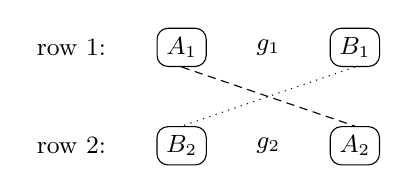
\begin{tikzpicture}[every node/.style={font=\small},baseline=(current bounding box.center)]
\node at (0,0.9) {row 1:};
\node[draw,rounded corners] (aa) at (1.4,0.9) {$A_1$};
\node at (2.5,0.9) {$g_1$};
\node[draw,rounded corners] (ba) at (3.6,0.9) {$B_1$};
\node at (0,-0.35) {row 2:};
\node[draw,rounded corners] (bb) at (1.4,-0.35) {$B_2$};
\node at (2.5,-0.35) {$g_2$};
\node[draw,rounded corners] (ab) at (3.6,-0.35) {$A_2$};
\draw[densely dashed] (aa.south) -- (ab.north);
\draw[dotted] (ba.south) -- (bb.north);
\end{tikzpicture}
\caption{Two owners $A,B$ contribute interleaving blocks to two
root components.  The order $A_1,B_1$ in row 1 is reversed as
$B_2,A_2$ in row 2; all row products must be preserved simultaneously.}
\label{fig:interleaved-blocks}
\end{figure}

\section{Preliminaries}
\label{sec:prelim}

Throughout, $\Sigma$ is a finite alphabet, $\eps$ the empty word and
$\Sigma^+:=\Sigma^*\setminus\{\eps\}$.  If $\Sigma=\emptyset$, the only
languages are $\emptyset$ and $\{\eps\}$ and are handled directly.  For a
finite $K\subseteq\Sigma^*$ put $\|K\|_+:=\sum_{w\in K}(|w|+1)$, and for a
tuple $\tuple u=(u_1,\ldots,u_d)$ put $\|\tuple u\|_1:=\sum_i|u_i|$.  Every
polynomial bound below states whether it concerns cardinality or
$\|\cdot\|_+$.  We use $G$ for a reduced good presentation and $G_{\mathrm{in}}$ for
an arbitrary input grammar; $\|G\|$, $\theta_G$ and $t_G$ denote
its encoding size, rule thickness and nonterminal thickness.
The fresh-identity completion of $s$ is $\widehat s$.
Section~\ref{sec:char-data} defines the shortest typed yield
$t_{\mathrm{typ}}$, representative length $\tau$ and shortest
realized type length $\mu_m$, none of which is rule thickness.

\subsection{Positive-Data Learning}

\begin{definition}[Text, TxtEx identification, conservativeness]
Fix a pause symbol $\pausesym\notin\Sigma$.  A \emph{text} for
$L\subseteq\Sigma^*$ is an infinite sequence over $L\cup\{\pausesym\}$ in which
every element of $L$ occurs; the \emph{content} of a finite prefix is the set
of elements of $\Sigma^*$ occurring in it.  A \emph{learner} is a computable map
from finite prefixes to grammars.  It \emph{TxtEx-identifies} $L$~\cite{Gold1967}
if on every text for $L$ its outputs are, from some stage on, one fixed grammar
$H$ with $L(H)=L$; it TxtEx-identifies a class if it does so for each member.
It is \emph{conservative} if it changes its hypothesis only on a datum
$w\in\Sigma^*$ not generated by the current hypothesis.  We fix a hypothesis
$H_0$ with $L(H_0)=\emptyset$.
\end{definition}

\begin{definition}[Set-driven operator and characteristic sample]
\label{def:characteristic-sample}
A \emph{set-driven reconstruction operator} $\mathcal B$ maps each finite
$K\subseteq\Sigma^*$ to a grammar $\mathcal B(K)$ depending only on the set
$K$; it is \emph{sample-consistent} if $K\subseteq L(\mathcal B(K))$ for all
$K$.  A finite $\mathcal F\subseteq L$ is a \emph{characteristic sample for
$\mathcal B$ and $L$} if $L(\mathcal B(K))=L$ for every finite $K$ with
$\mathcal F\subseteq K\subseteq L$ (cf.~\cite{deLaHiguera1997}).
\end{definition}

The definition constrains generated languages only: $\mathcal B(K)$ need not
stabilize syntactically as $K$ grows.

\subsection{Fixed Finite-Semigroup Typing}
\label{subsec:semigroup-typing}

\begin{definition}[Typing, fresh completion, refinement]
\label{def-monoid-morphism}
\label{def:semigroup-typing}
\label{def:h-refinement}
A \emph{typing} is a surjective semigroup morphism
$s:\Sigma^+\twoheadrightarrow\mathsf S$ onto a finite semigroup, given by the
multiplication table of $\mathsf S$ and the images of the letters, so that
$s(w)$ is computable in time $O(|w|)$; $\mathsf S$ is its \emph{positive
image}.  (A morphism into a larger finite semigroup is replaced by its
corestriction to the image.)  Let $\mathsf S^\sharp:=\mathsf
S\uplus\{\mathbf1_\sharp\}$ be obtained by adjoining a \emph{fresh} identity,
even if $\mathsf S$ already has one, and let
$\widehat{s}:\Sigma^*\twoheadrightarrow\mathsf S^\sharp$ be the monoid morphism
with $\widehat{s}(\eps)=\mathbf1_\sharp$ and $\widehat{s}|_{\Sigma^+}=s$.  For
$\tuple w\in(\Sigma^*)^d$ put
$\widehat{s}^{(d)}(\tuple w):=(\widehat{s}(w_1),\ldots,\widehat{s}(w_d))$; on
$(\Sigma^+)^d$ this is $s^{(d)}(\tuple w)$.  For typings $s,s'$ write $s\preceq
s'$ if $\ker s'\subseteq\ker s$ on $\Sigma^+$, and let $(s,s')$ be the typing
$w\mapsto(s(w),s'(w))$ onto its image in $\mathsf S\times\mathsf T$, where $\mathsf T:=s'(\Sigma^+)$; thus
$s,s'\preceq(s,s')$.  Write $s_{\mathrm{triv}}$ for the one-element typing.
\end{definition}

The fresh completion evaluates grammar templates (including empty
terminal gaps) and types tuple yields in the refinement of
Section~\ref{sec:refinement}; its new identity is not a positive-word type.
Algebraic conditions such as $\mathbf{LG}$ concern $\mathsf S$, not
$\mathsf S^\sharp$; indeed $\mathsf S^\sharp$ is never a local group, since
$\{\mathbf1_\sharp,e\}\cong U_1$ for any idempotent $e$ of the minimal ideal of $\mathsf S$.  A finite-monoid morphism $q:\Sigma^*\to\mathsf N$ determines
the positive typing $q|_{\Sigma^+}$: by
Lemma~\ref{lem:semigroup-transfer}(i), it gives the same target class and
set-driven reconstruction rules as the fresh completion of that typing.
Lemma~\ref{lem:semigroup-transfer}(ii) additionally identifies their
trimmed yield-type refinements for \emph{good} grammars.  This last
identification is not asserted for arbitrary standard grammars with
empty-component yields.

\begin{definition}[Prefix--suffix typing]
\label{def:prefix-suffix-typing}
For $k,\ell\ge0$ put $m_0:=\max\{1,k+\ell\}$, and for $|w|\ge m_0$ let
$\operatorname{pref}_k(w)$, $\operatorname{suf}_\ell(w)$ be the prefix and
suffix of the indicated lengths (length-zero windows are $\eps$).  Define
\[
 \widehat{s}_{k,\ell}(w)=
 \begin{cases}
   w, & |w|<m_0,\\
   \langle\operatorname{pref}_k(w),\operatorname{suf}_\ell(w)\rangle,
      & |w|\ge m_0,
 \end{cases}
\]
with disjoint tags for short words and pairs, and put
$M_{k,\ell}:=\widehat{s}_{k,\ell}(\Sigma^*)$.  For short $x,y$ and pairs
$\langle u,v\rangle,\langle u',v'\rangle$ define
\[
\begin{aligned}
 x\cdot y&:=\widehat{s}_{k,\ell}(xy), &
 x\cdot\langle u,v\rangle&:=\langle\operatorname{pref}_k(xu),v\rangle,\\
 \langle u,v\rangle\cdot y&:=\langle u,\operatorname{suf}_\ell(vy)\rangle, &
 \langle u,v\rangle\cdot\langle u',v'\rangle&:=\langle u,v'\rangle.
\end{aligned}
\]
Put $s_{k,\ell}:=\widehat{s}_{k,\ell}|_{\Sigma^+}$; a typing $s$ with
$s\preceq s_{k,\ell}$ for some $k,\ell\ge0$ is a \emph{window typing}.
\end{definition}

A case check on the lengths of $x,y\in\Sigma^*$ gives
$\widehat{s}_{k,\ell}(xy)=\widehat{s}_{k,\ell}(x)\cdot\widehat{s}_{k,\ell}(y)$.
Since $\widehat{s}_{k,\ell}$ is onto $M_{k,\ell}$, the product is associative
and $\widehat{s}_{k,\ell}(\eps)$ is an identity, so $\widehat{s}_{k,\ell}$ is a
finite-monoid morphism.  The short-word tag separates $\eps$ from
$\widehat{s}_{k,\ell}(\Sigma^+)$, so $\widehat{s}_{k,\ell}$ is isomorphic to the
completion $\widehat{s_{k,\ell}}$.

\subsection{Multiple Context-Free Grammars}

\begin{definition}[Standard MCFG presentation and size]
\label{def:standard-mcfg}
An MCFG \cite{SekiEtAl1991,Kallmeyer2010} is
$G=(V,\Sigma,P,S,\fan)$ with finite $V$, $S\in V$, $\fan(S)=1$ and
$\fan(A)\ge1$.  A rule of rank $r\ge0$ is
$A\to\rho(B_1,\ldots,B_r)$ with template
$\rho=(\alpha_1,\ldots,\alpha_{d_0})$, $d_0=\fan(A)$, $d_j=\fan(B_j)$, where
each $\alpha_i$ is a word over
$\Gamma_\rho:=\Sigma\uplus\Xi_1\uplus\cdots\uplus\Xi_r$,
$\Xi_j:=\{\xi_j^1,\ldots,\xi_j^{d_j}\}$, and every variable occurs at most once
in $\alpha_1\cdots\alpha_{d_0}$ (\emph{linearity}).  For $\tuple u_j\in(\Sigma^*)^{d_j}$,
$\rho(\tuple u_1,\ldots,\tuple u_r)$ substitutes $u_{j,\kappa}$ for
$\xi_j^\kappa$; for $r=0$ the rule is a \emph{constant rule}.  The tuple
languages $L_A(G)\subseteq(\Sigma^*)^{\fan(A)}$ form the least family closed
under the rules, and $L(G):=\{w:(w)\in L_S(G)\}$.  We write
$A\Rightarrow_G^*\tuple u$ for a \emph{terminal derivation} (a finite derivation
tree rooted at $A$, evaluated bottom-up); one from $S$ is \emph{successful}.
$G$ is an $f$-MCFG if $\fan(A)\le f$ for all $A$, and has rule-rank cap
$r_{\max}$ if all ranks are at most $r_{\max}$.  Such a presentation, with no
further restriction, is called \emph{standard}.  Its \emph{size} is
\[
 \|G\|:=|V|+\sum_{(A\to\rho(B_1,\ldots,B_r))\in P}
 \Bigl(1+r+\textstyle\sum_{i}|\alpha_i|\Bigr),
\]
where $|\alpha_i|$ counts terminal and variable occurrences.  All
bounds use this symbol-level size; a bit-level encoding with binary
nonterminal names changes it by at most a factor $O(\log\|G\|)$.
\end{definition}

$\mathsf{MCFL}(f,r)$ is the class of languages of MCFGs of fan-out $\le f$ and
rule rank $\le r$; $f\text{-}\mathrm{MCFL}=\bigcup_{r<\infty}\mathsf{MCFL}(f,r)$,
and the minimum rule rank of a language is taken over all its fan-out-$\le f$
presentations.  For nonterminals of equal fan-out $d$, $A\to B$ abbreviates
$A\to(\xi_1^1,\ldots,\xi_1^d)(B)$, and $A\to\tuple c$ a constant rule.  Rule
variables are always $\xi_j^\kappa$; terminals in examples are in
\texttt{typewriter} font.  Fan-out and rank are distinct resources.  At fixed fan-out at least
two the rule-rank hierarchy does not collapse in general, although adjacent
levels can coincide; in particular
$\mathsf{MCFL}(2,2)=\mathsf{MCFL}(2,3)$
\cite{RambowSatta1999,GomezRodriguezEtAl2009}.  By contrast, fan-out-one
CFGs can be binarized.  The reconstruction below therefore assumes neither
a binary normal form nor a known rank cap.

\begin{definition}[Grammar properties]
\label{def:grammar-properties}
A rule is \emph{nondeleting} if every variable occurs exactly once in its
template; a nondeleting rule is \emph{nonpermuting} if for each $j$ the
variables $\xi_j^1,\ldots,\xi_j^{d_j}$ occur in this order in
$\alpha_1\cdots\alpha_{d_0}$, and \emph{nonmerging} if moreover no $\alpha_i$
contains a factor $\xi_j^\kappa\xi_j^{\kappa+1}$.  Following
\cite[Section~2.3]{Yoshinaka2011}, a rule is \emph{$\eps$-free} (``$\lambda$-free''
there) if no $\alpha_i$ is empty.  A rule, template or grammar is \emph{good} if it is
$\eps$-free, nondeleting, nonpermuting and nonmerging.  A nonterminal $A$
is \emph{reachable} if there is a chain $S=A_0,\ldots,A_m=A$ in which each
$A_{i+1}$ is a child in a rule for $A_i$, and \emph{productive} if
$L_A(G)\ne\emptyset$; $G$ is \emph{reduced} if every nonterminal is both.
\end{definition}

In a $\eps$-free grammar every component of every derived tuple is nonempty
(induction on derivations).  $\eps$-freeness concerns template components
and is distinct from $\eps\notin L(G)$.

\subsection{Tuple Contexts and Substitutability}

A \emph{sentence context of arity $d$} is a word
$E=v_0\blank_1v_1\cdots v_{d-1}\blank_dv_d$ with each hole occurring once,
$v_0,v_d\in\Sigma^*$ and $v_1,\ldots,v_{d-1}\in\Sigma^+$; $\mathcal E_d$ is the
set of these \emph{admissible} contexts \cite[Section~3.1]{Yoshinaka2011}.
$E[\tuple w]$ fills $\blank_i$ by $w_i$, $|E|_{\mathrm{fix}}:=\sum_{i=0}^d|v_i|$,
and $E$ \emph{accepts} $\tuple w$ in $L$ if $E[\tuple w]\in L$.  The
\emph{$d$-tuple distribution} of $\tuple x\in(\Sigma^*)^d$ is
$\D_L^{(d)}(\tuple x):=\{E\in\mathcal E_d:E[\tuple x]\in L\}$; at fan-out one
it is the two-sided distribution $\{(u,v):uxv\in L\}$.

\begin{definition}[Tuple occurrence]
\label{def:tuple-occurrence}
For $w=a_1\cdots a_n$ number the cut positions
$\cutpos{0}a_1\cutpos{1}\cdots a_n\cutpos{n}$ and write
$w[i:i']:=a_{i+1}\cdots a_{i'}$.  An \emph{arity-$d$ tuple occurrence} in $w$
is a sequence $0\le i_1<i_1'<i_2<i_2'<\cdots<i_d<i_d'\le n$; it determines
$\tuple x=(w[i_1:i_1'],\ldots,w[i_d:i_d'])\in(\Sigma^+)^d$ and the context
$E\in\mathcal E_d$ obtained by replacing these intervals by
$\blank_1,\ldots,\blank_d$, so that $E[\tuple x]=w$.  For finite $K$,
$\mathrm{Obs}_d(K):=\{\tuple x\in(\Sigma^+)^d:E[\tuple x]\in K\text{ for some
}E\in\mathcal E_d\}$ is the set of tuples arising from such occurrences, and
for a fixed fan-out bound $f\ge1$, put
$\mathrm{Obs}(K):=\bigcup_{1\le d\le f}\mathrm{Obs}_d(K)$.
\end{definition}

\begin{definition}[$(f,s)$-tuple substitutability and the target class]
\label{def:tuple-substitutable}
\label{def:class-cmcf}
Let $f\ge1$ and let $s$ be a typing.  A language $L\subseteq\Sigma^*$ is
\emph{$(f,s)$-tuple-substitutable} if for every $1\le d\le f$ and all
$\tuple x,\tuple y\in(\Sigma^+)^d$,
\[
 s^{(d)}(\tuple x)=s^{(d)}(\tuple y)\ \text{ and }\
 \D_L^{(d)}(\tuple x)\cap\D_L^{(d)}(\tuple y)\ne\emptyset
 \ \Longrightarrow\
 \D_L^{(d)}(\tuple x)=\D_L^{(d)}(\tuple y).
\]
$\Cmcf{f}{s}$ is the class of $(f,s)$-tuple-substitutable $f$-MCFLs.  For
$\tuple x,\tuple y\in(\Sigma^+)^d$ write $\tuple x\equiv_{L,s}^d\tuple y$ (or
$\tuple x\equiv_{L,s}\tuple y$) if $s^{(d)}(\tuple x)=s^{(d)}(\tuple y)$ and
$\D_L^{(d)}(\tuple x)=\D_L^{(d)}(\tuple y)$; this is an equivalence relation.
\end{definition}

Empty components are never compared, following
\cite[Section~3.1 and footnote~3]{Yoshinaka2011} (see \cite{Clark2013} for
CFGs), and $\eps\in L$ is handled at the start symbol; otherwise already
$\mathtt a^+$ would fail, since $\mathtt a$ and $\eps$ share a context but not
their distributions.  The bias consists of both $s$ and $f$:
\begin{enumerate}[label=\textup{(\alph*)},leftmargin=*]
\item If $s\preceq s'$, equal $s'$-types are equal $s$-types, so
$\Cmcf{f}{s}\subseteq\Cmcf{f}{s'}$; in particular
$\Cmcf{f}{s_{\mathrm{triv}}}\subseteq\Cmcf{f}{s}$.  This compares classes
only: the operators $\mathcal B_{f,s}$ and $\mathcal B_{f,s'}$ of
Section~\ref{sec:learner} differ in general (they coincide when
$\ker s=\ker s'$).
\item $\Cmcf{f+1}{s}\cap f\text{-}\mathrm{MCFL}\subseteq\Cmcf{f}{s}$, but the
class is not monotone in $f$: for the trivial typing
$\{w\mathtt{\#}w^R:w\in\{\mathtt a,\mathtt b\}^*\}$ is
$1$- but not $2$-dimensionally substitutable
\cite[Section~3.1, Example~5]{Yoshinaka2011}.
\item For every $\mathsf{Acc}\subseteq\mathsf S^\sharp$,
$\widehat{s}^{-1}(\mathsf{Acc})\in\Cmcf{f}{s}$: it is regular, and
componentwise equal types give equal total types in every context.
\end{enumerate}

\begin{proposition}[Intersection and abelian filtering]
\label{prop:abelian-coset-filter}
Fix $f$ and $s$.
\begin{enumerate}[label=(\roman*),leftmargin=*]
\item If $L_1,L_2$ are $(f,s)$-tuple-substitutable, so is $L_1\cap L_2$.
\item If $L$ is $(f,s)$-tuple-substitutable, $\mathsf A$ is an abelian group,
$g:\Sigma^*\to\mathsf A$ a monoid morphism, $\mathsf H\le\mathsf A$ and
$\gamma\in\mathsf A$, then $L\cap g^{-1}(\gamma+\mathsf H)$ is
$(f,s)$-tuple-substitutable.
\item If $L\in\Cmcf{f}{s}$, $\mathsf{Acc}\subseteq\mathsf S^\sharp$ and, in (ii),
$\mathsf A$ is finite, then
$L\cap\widehat{s}^{-1}(\mathsf{Acc})\cap g^{-1}(\gamma+\mathsf H)\in\Cmcf{f}{s}$.
\end{enumerate}
For infinite $\mathsf A$ the intersection in (ii) belongs to $\Cmcf{f}{s}$ whenever
it is an $f$-MCFL.
\end{proposition}

\begin{proof}
(i) A context accepting equal-type $\tuple x,\tuple y$ in $L_1\cap L_2$ accepts
both in each $L_i$, so their distributions agree in each $L_i$, hence in the
intersection.  (ii) If some context $E$ accepts $\tuple x,\tuple y$ in
$g^{-1}(\gamma+\mathsf H)$, then
$\delta:=\sum_i(g(y_i)-g(x_i))\in\mathsf H$, and by commutativity
$g(E'[\tuple y])-g(E'[\tuple x])=\delta$ for every
$E'\in\mathcal E_d$, so coset membership transfers in both directions.  Thus
$g^{-1}(\gamma+\mathsf H)$ is $(f,s_{\mathrm{triv}})$-, hence
$(f,s)$-tuple-substitutable; apply (i).  (iii) The language
$\widehat{s}^{-1}(\mathsf{Acc})$ is $(f,s)$-tuple-substitutable by item (c) above,
so the intersection is, by (i) and (ii); it is the intersection of an $f$-MCFL with
a regular language, hence an $f$-MCFL \cite{SekiEtAl1991}.
\end{proof}

The factorizations in (ii) and (iii) are a tool for constructing members of the
class; they are not supplied to the reconstruction.

\section{Reconstruction and Qualitative Learning}
\label{sec:learner}

This section instantiates Yoshinaka's finite-signature reconstruction
\cite{Yoshinaka2015General} for $s$-refined MCFG tuple sorts.
Our soundness, completeness, exact-reconstruction and Gold-identification
claims (Propositions~\ref{prop:reconstruction-soundness},
\ref{prop:completeness}, Theorem~\ref{thm:exact-reconstruction},
Corollary~\ref{cor:gold-explanatory}) are qualitative analogues of
\cite[Lemmas~2--3 and Theorem~1]{Yoshinaka2015General},
not new results.  Appendices~\ref{app:qualitative-construction-details}
and~\ref{app:typed-witness-aux-proofs} prove them directly for the
concrete grammar; a sample-dependent rank cap handles unbounded
minimum rank.  Here the new question concerns total word length,
rather than the finite-signature bound on the number of words.

\subsection{Set-Driven Reconstruction}

All interaction between templates and contexts rests on one observation.

\begin{lemma}[Induced child contexts]
\label{lem:filling-identity}
Let $\rho=(\alpha_1,\ldots,\alpha_{d_0})$ be a good template of rank $r$ with child
arities $d_1,\ldots,d_r$, let $E\in\mathcal E_{d_0}$, let $1\le j\le r$, and fix
$\tuple u_i\in(\Sigma^+)^{d_i}$ for $i\ne j$.  Let $E_j$ be the word obtained
from $E[(\alpha_1,\ldots,\alpha_{d_0})]$ by replacing $\xi_j^\kappa$ by
$\blank_\kappa$ and every other variable $\xi_i^{\kappa'}$ by $u_{i,\kappa'}$.  Then
$E_j\in\mathcal E_{d_j}$ and
$E_j[\tuple x]=E[\rho(\tuple u_1,\ldots,\tuple u_{j-1},\tuple x,
\tuple u_{j+1},\ldots,\tuple u_r)]$ for every
$\tuple x\in(\Sigma^*)^{d_j}$.
\end{lemma}

If $L(G)=L\cap\Sigma^+$, then on nonempty tuple components
$\D_L^{(d)}$ agrees with $\D_{L(G)}^{(d)}$: for admissible $E$
the filled word $E[\tuple x]$ is always nonempty.
Consequently Lemma~\ref{lem:typed-homogeneity} also applies with
$L$ in place of $L(G)$.


\begin{lemma}[Composition preserves equivalence]
\label{lem:witnessed-composition}
Let $L\subseteq\Sigma^*$, let $\rho$ be a good template of rank $r$, and let
$\tuple x_j,\tuple u_j\in(\Sigma^+)^{d_j}$ satisfy
$\tuple u_j\equiv_{L,s}\tuple x_j$ for every $j$.  Then
$\rho(\tuple u_1,\ldots,\tuple u_r)\equiv_{L,s}\rho(\tuple x_1,\ldots,\tuple x_r)$.
\end{lemma}

\begin{definition}[Composition witness]
\label{def:composition-witness}
Let $K$ be finite and $r\ge1$.  A \emph{composition witness of rank $r$} in $K$
is a triple $(\tuple z,\rho,(\tuple u_1,\ldots,\tuple u_r))$ in which $\rho$
is a good template of rank $r$ with output arity $d_0\le f$ and child arities
$d_1,\ldots,d_r\le f$, $\tuple z\in\mathrm{Obs}_{d_0}(K)$,
$\tuple u_j\in(\Sigma^+)^{d_j}$, and
$\tuple z=\rho(\tuple u_1,\ldots,\tuple u_r)$.
\end{definition}

Equivalently, a composition witness is a segmentation of the components of an
observed $\tuple z$ into terminal gaps and nonempty intervals labelled by
variables, subject to the good-template conditions.  If $E[\tuple z]\in K$,
Lemma~\ref{lem:filling-identity} gives $E_j[\tuple u_j]=E[\tuple z]\in K$ with
$E_j$ admissible, so every $\tuple u_j\in\mathrm{Obs}(K)$.  The children occupy
disjoint, nonempty parts of $\tuple z$, so
\begin{equation}
\label{eq:sample-rank}
 r\le\textstyle\sum_j\|\tuple u_j\|_1\le\|\tuple z\|_1\le\max_{w\in K}|w|
 \le\|K\|_+ .
\end{equation}

\begin{definition}[Capped and uncapped reconstruction operators]
\label{def:reconstruction}
Fix $f$ and a typing $s$.  For $r_{\max}\ge1$ let
$\mathcal B_{f,s}^{\le r_{\max}}(K)=\widehat G_{\le r_{\max}}(K)$ be the
grammar with start symbol $\widehat S$, a nonterminal $[\tuple x]$ of arity
$d$ for each $\tuple x\in\mathrm{Obs}_d(K)$, $1\le d\le f$, and the rules
\begin{enumerate}[leftmargin=*]
\item[\textnormal{(Start)}] $\widehat S\to[(w)]$ for $w\in K\cap\Sigma^+$, and
      $\widehat S\to\eps$ if $\eps\in K$;
\item[\textnormal{(Const)}] $[\tuple x]\to\tuple x$ for every
      $\tuple x\in\mathrm{Obs}(K)$;
\item[\textnormal{(Comp)}] $[\tuple z]\to\rho([\tuple u_1],\ldots,[\tuple u_r])$
      for every composition witness of rank $1\le r\le r_{\max}$;
\item[\textnormal{(Link)}] $[\tuple x]\to[\tuple y]$ for
      $\tuple x,\tuple y\in\mathrm{Obs}_d(K)$ with
      $s^{(d)}(\tuple x)=s^{(d)}(\tuple y)$ and $E[\tuple x],E[\tuple y]\in K$
      for some $E\in\mathcal E_d$.
\end{enumerate}
For $K\ne\emptyset$ put $\mathcal B_{f,s}(K):=\widehat G(K):=
\widehat G_{\le\|K\|_+}(K)$; $\mathcal B_{f,s}(\emptyset)$ has no rules.
Fixed encoding orders make both operators deterministic and set-driven.
\end{definition}

By \eqref{eq:sample-rank}, $\mathcal B_{f,s}(K)$ contains a Comp rule for every
composition witness in $K$.  Both operators are sample-consistent, via
$\widehat S\to[(w)]\to(w)$ and $\widehat S\to\eps$.  All non-start templates
are $\eps$-free, so $\widehat S\Rightarrow^*\eps$ only by the rule
$\widehat S\to\eps$.  For the trivial typing and $\eps\notin K$, Comp/Const, Link
and Start correspond to the rules of Types~I--III of
\cite[Section~4.1]{Yoshinaka2011}, and $\mathcal B_{f,s}$ corresponds to the
operator of the unbounded-rank learner
$\mathcal A(p,*)$ of \cite[Corollary~2]{Yoshinaka2011}.

\subsection{Yield-Typed Refinement and Witnesses}
\label{sec:refinement}

\begin{definition}[Yield-type refinement]
\label{def:output-refinement}
Let $G=(V,\Sigma,P,S,\fan)$ be a finite nondeleting MCFG and $s$ a typing.
For a template $\rho$ and $\mathbf t_j\in(\mathsf S^\sharp)^{d_j}$, let
$\out_\rho(\mathbf t_1,\ldots,\mathbf t_r)\in(\mathsf S^\sharp)^{d_0}$ have
$i$th component the image of $\alpha_i$ under the monoid morphism
$\Gamma_\rho^*\to\mathsf S^\sharp$ extending $a\mapsto\widehat{s}(a)$ and
$\xi_j^\kappa\mapsto(\mathbf t_j)_\kappa$.  The \emph{full yield-type
refinement} $G^{\widehat{s}}$ has a fresh start symbol $\widetilde S$,
nonterminals $A_{\mathbf t}$ for $A\in V$ and
$\mathbf t\in(\mathsf S^\sharp)^{\fan(A)}$, start rules
$\widetilde S\to S_{(m)}$ for $m\in\mathsf S^\sharp$, and for every rule
$A\to\rho(B_1,\ldots,B_r)$ (including $r=0$) and all
$\mathbf t_j\in(\mathsf S^\sharp)^{\fan(B_j)}$ the rule
$A_{\out_\rho(\mathbf t_1,\ldots,\mathbf t_r)}\to
\rho(B_{1,\mathbf t_1},\ldots,B_{r,\mathbf t_r})$.  The \emph{trimmed
refinement} $\widetilde G_0$ keeps exactly the nonterminals and rules occurring
in some successful derivation from $\widetilde S$.  Unless $G^{\widehat{s}}$ is
named, \emph{typed nonterminals} and \emph{typed rules} are the non-start
nonterminals and rules of $\widetilde G_0$, and
$L_X:=\{\tuple u:X\Rightarrow_{\widetilde G_0}^*\tuple u\}$.
\end{definition}

Typed rules have the templates of their sources, so $\widetilde G_0$ is good
whenever $G$ is; each $L_X$ is nonempty, and its tuples have nonempty
components if $G$ is $\eps$-free.

\begin{proposition}[Yield-type invariants]
\label{prop:output-invariants}
\begin{enumerate}[label=(\roman*),leftmargin=*]
\item If $A_{\mathbf t}\Rightarrow^*\tuple u$ in $G^{\widehat{s}}$, then
$\widehat{s}^{(\fan(A))}(\tuple u)=\mathbf t$, and erasing indices gives a
$G$-derivation of $\tuple u$.
\item Every terminal derivation $A\Rightarrow_G^*\tuple u$ lifts uniquely to
$A_{\widehat{s}^{(\fan(A))}(\tuple u)}\Rightarrow_{G^{\widehat{s}}}^*\tuple u$; a successful
derivation of $w$ lifts uniquely through $\widetilde S\to S_{(\widehat{s}(w))}$.
\item $L(\widetilde G_0)=L(G^{\widehat{s}})=L(G)$.
\item For every typed nonterminal $X$, every terminal derivation
$X\Rightarrow^*_{G^{\widehat s}}\tuple u$ uses only rules of $\widetilde G_0$; hence
$L_X=\{\tuple u:X\Rightarrow^*_{G^{\widehat s}}\tuple u\}$.
\end{enumerate}
\end{proposition}

\begin{lemma}[Canonical contexts for typed nonterminals]
\label{lem:identity-canonical-contexts}
Let $G$ be good.  Every typed nonterminal $X$ of arity $d$ has a context
$\chi(X)\in\mathcal E_d$ with $\chi(X)[\tuple u]\in L(G)$ for all
$\tuple u\in L_X$; if $\widetilde S\to X$ is in $\widetilde G_0$, one may take
$\chi(X)=\blank_1$.
\end{lemma}

\begin{lemma}[Typed nonterminals are distributionally homogeneous]
\label{lem:typed-homogeneity}
Let $G$ be good of fan-out $\le f$ with $L:=L(G)\in\Cmcf{f}{s}$.  For every typed nonterminal $X$
of arity $d$, $L_X$ lies in a single $\equiv_{L,s}^d$-class, denoted
$\operatorname{Cl}_{L,s}(X)$.
\end{lemma}

The semantic class $\operatorname{Cl}_{L,s}(X)$ is distinct from the syntactic
reconstruction nonterminal $[\tuple x]$ of Definition~\ref{def:reconstruction}.

The proofs of these three statements are in
Appendix~\ref{app:typed-witness-aux-proofs}.  The homogeneity of
Lemma~\ref{lem:typed-homogeneity} is weaker than that of congruential
MCFGs~\cite{ClarkYoshinaka2016}, whose contexts may have empty separators.

\begin{definition}[Canonical tuples, contexts and the witness set]
\label{def:target-canonical}
\label{def:witness-set}
Let $G$ be good.  For every typed nonterminal $X$ fix a \emph{canonical tuple}
$\omega(X)\in L_X$ and a \emph{canonical context} $\chi(X)$ as in
Lemma~\ref{lem:identity-canonical-contexts}, with $\chi(X)=\blank_1$ whenever
$\widetilde S\to X$ is in $\widetilde G_0$.  Let $\Wit(\widetilde G_0)$
consist of the words
\[
 \chi(X)[\omega(X)]\ \ (X\text{ typed}),\qquad
 \chi(X)[\rho(\omega(Y_1),\ldots,\omega(Y_q))]\ \
 (X\to\rho(Y_1,\ldots,Y_q)\text{ typed},\ q\ge0).
\]
\end{definition}

Since $\omega(X)$ and $\rho(\omega(Y_1),\ldots,\omega(Y_q))$ belong to $L_X$,
$\Wit(\widetilde G_0)$ is a finite subset of $L(G)$, nonempty if
$L(G)\ne\emptyset$, and $|\Wit(\widetilde G_0)|$ is at most the number of
typed nonterminals and rules.  Canonical objects are properties of the
target, not inputs of the operator: qualitatively any choice works, while
Section~\ref{sec:char-data} chooses short ones.

\subsection{Qualitative Guarantees}\label{sec:soundness}
\label{sec:completeness}
\label{sec:poly-time}

\begin{proposition}[Soundness of every hypothesis]
\label{prop:reconstruction-soundness}
Let $L$ be $(f,s)$-tuple-substitutable and $K\subseteq L$ finite.  For every
$r_{\max}\ge1$, if $[\tuple x]\Rightarrow^*\tuple u$ in
$\widehat G_{\le r_{\max}}(K)$, then $\tuple u\equiv_{L,s}\tuple x$.
Consequently $L(\mathcal B_{f,s}^{\le r_{\max}}(K))\subseteq L$ and
$L(\mathcal B_{f,s}(K))\subseteq L$.
\end{proposition}

\begin{proposition}[Completeness from a witness assignment]
\label{prop:completeness}
Let $G$ be a finite good MCFG of fan-out $\le f$, let $r_G$ be the maximum
rank of a typed rule of $\widetilde G_0$ ($r_G:=0$ if none), and assign to
each typed nonterminal $X=A_{\mathbf t}$ a tuple
$\iota(X)\in(\Sigma^+)^{\fan(A)}$ with $\widehat s^{(\fan(A))}(\iota(X))=\mathbf t$
and a context $\chi(X)\in\mathcal E_{\fan(A)}$, with $\chi(X)=\blank_1$ if
$\widetilde S\to X$ is in $\widetilde G_0$.  Suppose $K$ contains
$\chi(X)[\iota(X)]$ for each $X$ and
$\chi(X)[\rho(\iota(Y_1),\ldots,\iota(Y_q))]$ for each
typed rule $X\to\rho(Y_1,\ldots,Y_q)$, $q\ge0$.  Then
\[
 L(G)\subseteq L\bigl(\mathcal B_{f,s}^{\le r_{\max}}(K)\bigr)
 \quad(r_{\max}\ge\max\{1,r_G\}),\qquad
 L(G)\subseteq L\bigl(\mathcal B_{f,s}(K)\bigr).
\]
\end{proposition}

Neither substitutability nor $\iota(X)\in L_X$ is assumed in
Proposition~\ref{prop:completeness}; $\iota=\omega$ is the case
$\Wit(\widetilde G_0)\subseteq K$.

Exact reconstruction needs a good presentation of the target; the following
normalization controls size, fan-out and rank, but not thickness.  The rule
thickness of $G_{\mathrm{good}}$ may exceed that of $G_{\mathrm{in}}$, so all
data bounds below are stated relative to a given reduced good presentation and
are not transferred through normalization.

\begin{proposition}[Good normalization with rank preservation]
\label{prop:good-normalization}
Let $G_{\mathrm{in}}$ be a finite standard $f$-MCFG of rule rank at most
$r_{\max}$.  There is a finite good $f$-MCFG $G_{\mathrm{good}}$ of rule rank at
most $r_{\max}$ with $L(G_{\mathrm{good}})=L(G_{\mathrm{in}})\setminus\{\eps\}$
and, for fixed $f,r_{\max}$,
$\|G_{\mathrm{good}}\|=O_{f,r_{\max}}(\|G_{\mathrm{in}}\|)$.  If
$L(G_{\mathrm{in}})\cap\Sigma^+\ne\emptyset$, $G_{\mathrm{good}}$ is reduced.
\end{proposition}

\begin{theorem}[Exact reconstruction for a fixed typing]
\label{thm:exact-reconstruction}
Fix $f\ge1$ and a typing $s$, and let $L\in\Cmcf{f}{s}$.  If
$L\cap\Sigma^+=\emptyset$ put $\mathcal F_L:=L$ and $r_G:=0$.  Otherwise let $G$
be a reduced good fan-out-$\le f$ presentation of $L\cap\Sigma^+$
(Proposition~\ref{prop:good-normalization}), let $r_G$ be as in
Proposition~\ref{prop:completeness}, and put
$\mathcal F_L:=\Wit(\widetilde G_0)\cup(\{\eps\}\cap L)$.  Then
$\mathcal F_L\subseteq L$ is finite, and every finite $K$ with
$\mathcal F_L\subseteq K\subseteq L$ satisfies
\[
 L(\mathcal B_{f,s}(K))=L,\qquad
 L(\mathcal B_{f,s}^{\le r_{\max}}(K))=L\quad
 \text{for every }r_{\max}\ge\max\{1,r_G\}.
\]
If $L\in\mathsf{MCFL}(f,r)$, $G$ can be chosen of rank $\le r$, so
$r_{\max}=\max\{1,r\}$ suffices (also when $r=0$).
\end{theorem}

\begin{theorem}[Polynomial construction under a rule-rank cap]
\label{thm:poly}
Fix $f,r_{\max}\ge1$ and $s$.  The encoding of $\widehat G_{\le r_{\max}}(K)$ is
computable in time $(1+\|K\|_+)^{O(fr_{\max})}$; its fan-out is at most $f$
and its rank at most $r_{\max}$.
\end{theorem}

\begin{definition}[Conservative sequential learner]
\label{def:conservative-learner}
The learner $\mathcal A_{f,s}$ (respectively $\mathcal A_{f,s}^{\le r_{\max}}$)
starts with $H_0$, keeps its hypothesis on $\pausesym$ and on every datum the
hypothesis generates, and otherwise replaces it by $\mathcal B_{f,s}(K)$
(respectively $\mathcal B_{f,s}^{\le r_{\max}}(K)$), where $K$ is the content
read so far.  This is the policy of \cite[Algorithm~1]{Yoshinaka2011}.
\end{definition}

\begin{corollary}[Gold identification]
\label{cor:gold-explanatory}
\label{cor:capped-gold-poly}
Fix $f\ge1$ and $s$.
\begin{enumerate}[label=\textup{(\roman*)}]
\item $\mathcal A_{f,s}$ TxtEx-identifies $\Cmcf{f}{s}$.
\item For fixed $r_{\max}$, $\mathcal A_{f,s}^{\le r_{\max}}$ TxtEx-identifies
$\Cmcf{f}{s}\cap\mathsf{MCFL}(f,r_{\max})$, and processes each datum in time
polynomial in $\|K\|_+$ for the content $K$ read so far.
\end{enumerate}
\end{corollary}

Proofs are in Appendix~\ref{app:qualitative-construction-details}
(Proposition~\ref{prop:good-normalization}: Appendix~\ref{app:normalization-details}).
None of these statements bounds the length of characteristic data or the
stage of convergence.

\subsection{Typed versus Untyped Classes}
\label{subsec:typed-separation}

Regular path languages give simple members of every class.

\begin{lemma}[Path languages]\label{lem:app-lf-path}
Let $R$ be the set of labels of paths from a vertex $p$ to a vertex $p'$ in a
finite directed graph in which every letter labels exactly one edge.  If
$\tuple x,\tuple y\in(\Sigma^+)^d$ and $E\in\mathcal E_d$ satisfy
$E[\tuple x],E[\tuple y]\in R$, then $F[\tuple x]\in R\iff F[\tuple y]\in R$ for
every $F\in\mathcal E_d$.
\end{lemma}

\begin{proof}
A word of $\Sigma^+$ lies in $R$ iff the target of the edge of each letter is the
source of the edge of the next one, the first edge starts at $p$ and the last
ends at $p'$.  The $h$-th hole of $E$ is preceded by the last letter of
$v_{h-1}$, or by the vertex $p$ when $h=1$ and $v_0=\eps$, and is followed
likewise; internal separators are nonempty.  So $E$ determines the vertices at
both ends of each hole, and $x_h$ and $y_h$ label paths between the same two
vertices.  Replacing every $x_h$ by $y_h$ in $F[\tuple x]$ therefore preserves
all three conditions, and conversely.
\end{proof}

The class grows strictly with the typing already at fan-out two, and outside the
context-free languages; the untyped operator then over-generalizes.

\begin{proposition}[A typed class beyond the untyped one]
\label{prop:typed-separation}
Let $\Sigma=\{\mathtt a,\mathtt b,\mathtt c,\mathtt d,\mathtt\#_1,\mathtt\#_2,\mathtt\#_3\}$, let
$s:\Sigma^+\twoheadrightarrow\mathbb Z_2$ count the letters $\mathtt a$ and $\mathtt c$
modulo $2$, and let
\[
 L_{\mathrm{sep}}:=\{\mathtt a^m\mathtt\#_1\mathtt b^n\mathtt\#_2\mathtt c^{m'}\mathtt\#_3\mathtt d^n:
 m,n\ge0,\ m'\in\{m,m-1\},\ m'\ge0\}.
\]
\begin{enumerate}[label=\textup{(\roman*)},leftmargin=*]
\item $L_{\mathrm{sep}}$ is a $2$-MCFL of rule rank two and is not context-free.
\item $L_{\mathrm{sep}}$ is $(f,s)$-tuple-substitutable for every $f\ge1$; hence
$L_{\mathrm{sep}}\in\Cmcf{f}{s}$ for every $f\ge2$.
\item $L_{\mathrm{sep}}$ is not $(f,s_{\mathrm{triv}})$-tuple-substitutable for any $f\ge1$:
the words $\mathtt a$ and $\mathtt a\mathtt a$ share the context
$\blank_1\mathtt\#_1\mathtt\#_2\mathtt c\mathtt\#_3$ but not the context
$\blank_1\mathtt\#_1\mathtt\#_2\mathtt\#_3$.  Accordingly, on the sample
$K=\{\mathtt a\mathtt\#_1\mathtt\#_2\mathtt c\mathtt\#_3,\
\mathtt a\mathtt a\mathtt\#_1\mathtt\#_2\mathtt c\mathtt\#_3,\
\mathtt a\mathtt\#_1\mathtt\#_2\mathtt\#_3\}\subseteq L_{\mathrm{sep}}$ the untyped operator
$\mathcal B_{f,s_{\mathrm{triv}}}$ derives
$\mathtt a\mathtt a\mathtt\#_1\mathtt\#_2\mathtt\#_3\notin L_{\mathrm{sep}}$, whereas
$\mathcal B_{f,s}$ does not link $\mathtt a$ with $\mathtt a\mathtt a$.
\end{enumerate}
\end{proposition}

\begin{proof}
Let $\psi:\Sigma^*\to\mathbb Z^2$ be the morphism with $\psi(\mathtt a)=(1,0)$,
$\psi(\mathtt c)=(-1,0)$, $\psi(\mathtt b)=(0,1)$, $\psi(\mathtt d)=(0,-1)$ and
$\psi(\mathtt\#_i)=(0,0)$, and let
$R:=\mathtt a^*\mathtt\#_1\mathtt b^*\mathtt\#_2\mathtt c^*\mathtt\#_3\mathtt d^*$.  Then
$L_{\mathrm{sep}}=R\cap\psi^{-1}(P)$ with $P:=\{(0,0),(1,0)\}$, and $R$ is the path language
from $0$ to $3$ of the graph on $\{0,1,2,3\}$ with loops $\mathtt a,\mathtt b,\mathtt c,\mathtt d$
at $0,1,2,3$ and edges $\mathtt\#_h:h-1\to h$; every letter labels exactly one edge.

(i) The rules $E\to(\eps,\eps)\mid(\mathtt a\xi_1^1,\mathtt c\xi_1^2)(E)$,
$D\to(\eps,\eps)\mid(\mathtt b\xi_1^1,\mathtt d\xi_1^2)(D)$ and
\[
 S\to(\xi_1^1\mathtt\#_1\xi_2^1\mathtt\#_2\xi_1^2\mathtt\#_3\xi_2^2)(E,D)\mid
 (\mathtt a\xi_1^1\mathtt\#_1\xi_2^1\mathtt\#_2\xi_1^2\mathtt\#_3\xi_2^2)(E,D)
\]
form a standard MCFG of fan-out two and rule rank two generating $L_{\mathrm{sep}}$, since $E$
derives the pairs $(\mathtt a^k,\mathtt c^k)$ and $D$ the pairs $(\mathtt b^n,\mathtt d^n)$.
The words of $L_{\mathrm{sep}}$ in which $\mathtt a$ and $\mathtt c$ occur an even number of
times altogether are exactly those with $m'=m$; this is an intersection with a regular
language, and erasing the markers maps the result onto
$\{\mathtt a^m\mathtt b^n\mathtt c^m\mathtt d^n:m,n\ge0\}$, which is not context-free.  Context-free
languages are closed under both operations.

(ii) Let $1\le d\le f$, let $\tuple x,\tuple y\in(\Sigma^+)^d$ have equal componentwise
$s$-types, and let $E\in\mathcal E_d$ accept both.  Put
$(\delta_1,\delta_2):=\sum_i\bigl(\psi(x_i)-\psi(y_i)\bigr)=\psi(E[\tuple x])-\psi(E[\tuple y])
\in P-P$, so $\delta_2=0$ and $\delta_1\in\{-1,0,1\}$.  The first coordinate of $\psi$ is
congruent to $s$ modulo $2$ on every word, so $\delta_1$ is even; hence
$\psi(F[\tuple x])=\psi(F[\tuple y])$ for every $F\in\mathcal E_d$.  By
Lemma~\ref{lem:app-lf-path}, $F[\tuple x]\in R$ iff $F[\tuple y]\in R$.  So $F$ accepts
$\tuple x$ iff it accepts $\tuple y$.  With (i), $L_{\mathrm{sep}}\in\Cmcf{f}{s}$ for $f\ge2$.

(iii) The two contexts give
$\mathtt a\mathtt\#_1\mathtt\#_2\mathtt c\mathtt\#_3,\
\mathtt a\mathtt a\mathtt\#_1\mathtt\#_2\mathtt c\mathtt\#_3\in L_{\mathrm{sep}}$ ($m'=m$ and
$m'=m-1$), $\mathtt a\mathtt\#_1\mathtt\#_2\mathtt\#_3\in L_{\mathrm{sep}}$ and
$\mathtt a\mathtt a\mathtt\#_1\mathtt\#_2\mathtt\#_3\notin L_{\mathrm{sep}}$.  On $K$, the first
context gives the Link rule $[(\mathtt a)]\to[(\mathtt a\mathtt a)]$ for the trivial typing,
and $((\mathtt a\mathtt\#_1\mathtt\#_2\mathtt\#_3),(\xi_1^1\mathtt\#_1\mathtt\#_2\mathtt\#_3),
((\mathtt a)))$ is a composition witness of rank one, so
$\widehat S\to[(\mathtt a\mathtt\#_1\mathtt\#_2\mathtt\#_3)]\to[(\mathtt a)]\mathtt\#_1\mathtt\#_2
\mathtt\#_3\to[(\mathtt a\mathtt a)]\mathtt\#_1\mathtt\#_2\mathtt\#_3\to
\mathtt a\mathtt a\mathtt\#_1\mathtt\#_2\mathtt\#_3$.  Under $s$ the types of $\mathtt a$ and
$\mathtt a\mathtt a$ differ, so no such Link rule exists.
\end{proof}

The positive image of $s$ is the group $\mathbb Z_2$, a local group, so
Theorem~\ref{thm:A} gives $L_{\mathrm{sep}}$ characteristic data of length
$O(\|G\|^2\bar\theta_G)$ for each of its reduced good presentations
of rank at most $r_{\max}$, at every fixed fan-out $f\ge2$ (with the
constant depending only on $f$, $r_{\max}$ and $|\mathsf S|=2$),
while $L_{\mathrm{sep}}$ lies outside the class of Yoshinaka's untyped learner
\cite{Yoshinaka2011} at every fan-out.

\section{Characteristic-Data Bounds}
\label{sec:char-data}
Fix $f$, $r_{\max}$, $\Sigma$ and $s$, and a reduced good MCFG
$G=(V,\Sigma,P,S,\fan)$ with trimmed $\widehat s$-refinement
$\widetilde G_0$.  The reconstruction already has $O(\|G\|)$
characteristic words (Theorem~\ref{thm:exact-reconstruction});
we bound their total length in terms of $G$.
Lemma~\ref{lem:witness-length-template} converts short
same-type substitutes of nonterminal yields into a sample-length
bound.  Section~\ref{subsec:group-invariants} obtains the substitutes
by simultaneous shortening and heavy-node counting
(Lemma~\ref{lem:heavy-node-count}); local-group typings reduce to
sliding-factor coordinates (Section~\ref{subsec:algebraic-typed-data}).
The full type-refined grammar may be exponentially thicker than $G$
(Proposition~\ref{prop:typed-thickness-exponential}), so it is not
our complexity parameter.  Auxiliary proofs are in
Appendix~\ref{app:typed-witness-aux-proofs}.

\subsection{Thickness Scales and Witness Length}
\label{subsec:thickness-contexts}

For a rule $R$ of $G$ let
\[
 \theta_G(R):=\min\{\,|w|:w\in L(G)\text{ has a successful derivation using }R\,\},
\]
the length of the derived \emph{sentence}, not of the derivation.  Put
$\theta_G:=\max_{R\in P}\theta_G(R)$, $\bar\theta_G:=\max\{1,\theta_G\}$ and
$t_G:=\max_{A\in V}\min\{\|\tuple w\|_1:\tuple w\in L_A(G)\}$ (rule and
nonterminal thickness; $\theta_G$ is the thickness of
\cite[Section~4.3]{Yoshinaka2011}).

If a target $L$ contains $\eps$, every statement below is applied to
$L\cap\Sigma^+$ and the datum $\eps$ is added, as in
Theorem~\ref{thm:exact-reconstruction}; this adds one to the encoded length.

\begin{lemma}[Thickness lemma]
\label{lem:thickness-equivalence}
\label{lem:thickness-local-bounds}
\label{lem:untyped-contexts}
Let $G$ be reduced and good.
\begin{enumerate}[label=\textup{(\roman*)},leftmargin=*]
\item Every rule writes at most $\theta_G$ terminal symbols explicitly.
\item $t_G\le\theta_G$: every $A\in V$ has some $\tuple u\in L_A(G)$ with
$\|\tuple u\|_1\le\theta_G$.
\item $\theta_G\le 2\|G\|\max\{1,t_G\}$.
\item Every $A\in V$ of fan-out $d$ has a context $E_A\in\mathcal E_d$ with
$|E_A|_{\mathrm{fix}}\le\theta_G$ that results from a successful derivation by
deleting one occurrence of an $A$-subtree; $E_S=\blank_1$, and
$E_A[\tuple u]\in L(G)$ for all $\tuple u\in L_A(G)$.  For every typed nonterminal
$X=A_{\mathbf t}$, the choice $\chi(X):=E_A$ meets
Definition~\ref{def:target-canonical} and is \emph{derivational} for $X$: it
results from a successful derivation of $\widetilde G_0$ by deleting an
occurrence of an $X$-subtree.
\end{enumerate}
\end{lemma}

Thus $\theta_G$ and $t_G$ are polynomially equivalent on reduced good
presentations; Yoshinaka's efficiency criterion measures data in target size and
rule thickness \cite[Definition~1]{Yoshinaka2011}; see also
\cite{EyraudHeinzYoshinaka2016}.

For a finite-monoid morphism $\lambda:\Sigma^*\to\mathsf N$ we write $s\preceq\lambda$
if $\ker(\lambda|_{\Sigma^+})\subseteq\ker s$; since $\widehat s$ separates $\eps$,
this is the relation of Definition~\ref{def:semigroup-typing} whenever $\lambda$
also separates $\eps$ from $\Sigma^+$.  In that case we also write
$\widehat s\preceq\lambda$, meaning
$\ker\lambda\subseteq\ker\widehat s$ on all of $\Sigma^*$.
For $\beta\ge0$ consider
\begin{itemize}[leftmargin=4em]
\item[$(\mathrm R_\beta^\lambda)$] for every $B\in V$ and $\tuple u\in L_B(G)$
there is $\tuple u'\in L_B(G)$ with
$\lambda^{(\fan(B))}(\tuple u')=\lambda^{(\fan(B))}(\tuple u)$ and
$\|\tuple u'\|_1\le\beta$.
\end{itemize}
Put
\[
 C_s(G):=|V||\mathsf S^\sharp|^f+|P||\mathsf S^\sharp|^{fr_{\max}}
 \;\le\;|\mathsf S^\sharp|^{fr_{\max}}\,\|G\|,
\]
using $|V|+|P|\le\|G\|$; it bounds the numbers of typed nonterminals and typed
rules together, since a typed rule is determined by its source rule and the type
vectors of its at most $r_{\max}$ children.

\begin{lemma}[Witness length]
\label{lem:witness-length-template}
\label{lem:type-preserving-replacement}
Let $\lambda:\Sigma^*\to\mathsf N$ be a finite-monoid morphism with $s\preceq\lambda$.
\begin{enumerate}[label=\textup{(\roman*)},leftmargin=*]
\item \emph{(Type-preserving exchange.)}  If $X=B_{\mathbf t}$ is a typed
nonterminal, $\tuple u\in L_X$, $\tuple u'\in L_B(G)$ and
$\lambda^{(\fan(B))}(\tuple u')=\lambda^{(\fan(B))}(\tuple u)$, then
$\tuple u'\in L_X$.  Hence under $(\mathrm R_\beta^\lambda)$ there are canonical
tuples with $\|\omega(X)\|_1\le\beta$ for every $X$.
\item \emph{(Length.)}  Let $\chi(X):=E_B$ for $X=B_{\mathbf t}$, as in
Lemma~\ref{lem:thickness-equivalence}(iv), and let $\iota$ assign to every typed $X$ a
tuple $\iota(X)$ of nonempty words of its arity with $\|\iota(X)\|_1\le b$.  Let
$\Wit_\iota$ consist of the words $\chi(X)[\iota(X)]$ and
$\chi(X)[\rho(\iota(Y_1),\ldots,\iota(Y_q))]$ for typed rules
$X\to\rho(Y_1,\ldots,Y_q)$, $q\ge0$; thus $\Wit_\omega=\Wit(\widetilde G_0)$.  Every
word of $\Wit_\iota$ has length at most $2\bar\theta_G+r_{\max}b$, and
\[
 |\Wit_\iota|\le C_s(G),\qquad
 \|\Wit_\iota\|_+\le C_s(G)\,\bigl(1+2\bar\theta_G+r_{\max}b\bigr).
\]
\item \emph{(Refined thickness.)}  In (ii), each rule word
$\chi(X)[\rho(\omega(Y_1),\ldots,\omega(Y_q))]$ is the yield of a successful
derivation of $\widetilde G_0$ using the typed rule
$X\to\rho(Y_1,\ldots,Y_q)$; hence $\theta_{\widetilde G_0}\le2\bar\theta_G+r_{\max}b$.
\item \emph{(Characteristic sample.)}  Let $L(G)=L\cap\Sigma^+$ for some
$L\in\Cmcf{f}{s}$, and in \textup{(ii)} let $\iota(X)\in\operatorname{Cl}_{L,s}(X)$ for every
$X$ (Lemma~\ref{lem:typed-homogeneity}), for instance $\iota=\omega$.  Then
$\Wit_\iota\subseteq L$, and $\Wit_\iota\cup(\{\eps\}\cap L)$ is a characteristic
sample for $\mathcal B^{\le r_{\max}}_{f,s}$ and for $\mathcal B_{f,s}$.
\end{enumerate}
\end{lemma}

Items (i)--(iii) of Lemma~\ref{lem:witness-length-template} do not use
substitutability.

\subsection{Typed Thickness and Characteristic Data}
\label{subsec:typed-thickness}

Recall that $\widetilde G_0$ is the trimmed full yield-type refinement of $G$
(Definition~\ref{def:output-refinement}).  Define
\[
 t_{\mathrm{typ}}(G,s):=\max_{X}\min_{\tuple u\in L_X}\|\tuple u\|_1,
\]
where $X$ ranges over the non-start typed nonterminals, and let
$N_{\mathrm{typ}}(G,s)$ denote their number plus the number of non-start
typed rules.  In particular $N_{\mathrm{typ}}\le C_s(G)\le
|\mathsf S^\sharp|^{fr_{\max}}\|G\|$.

\begin{theorem}[Characteristic data from typed thickness]
\label{thm:data-from-typed-thickness}
Let $L\in\Cmcf{f}{s}$ and $G$ be a reduced good fan-out-$\le f$,
rank-$\le r_{\max}$ grammar with $L(G)=L\cap\Sigma^+$.
Take shortest canonical tuples and the derivational contexts $E_B$ of
Lemma~\ref{lem:thickness-equivalence}(iv).  Then
$K=\Wit(\widetilde G_0)\cup(\{\eps\}\cap L)$ is a characteristic sample
for both $\mathcal B^{\le r_{\max}}_{f,s}$ and $\mathcal B_{f,s}$, with
\[
 |\Wit(\widetilde G_0)|\le N_{\mathrm{typ}},\qquad
 \|\Wit(\widetilde G_0)\|_+\le
 N_{\mathrm{typ}}\bigl(1+2\bar\theta_G+r_{\max}t_{\mathrm{typ}}\bigr).
\]
For the full sample $K$, the length bound has the additional term
$\mathbf 1_{\{\eps\in L\}}$.
\end{theorem}

The numerical length estimate holds for any typing; substitutability is used
only for the characteristic-sample claim.

For the trivial typing, every nonterminal of the $\eps$-free $G$ has one
realized type vector, so $t_{\mathrm{typ}}=t_G$ and
$N_{\mathrm{typ}}=|V|+|P|\le\|G\|$.  The theorem recovers the
$O(\|G\|\bar\theta_G)$ untyped scale, although Yoshinaka's original
sample has the sharper bounds $|K_G|\le|P|$ and
$\|K_G\|\le|P|\theta_G$ \cite[Lemma~7 and Theorem~1]{Yoshinaka2011}.
A nontrivial typing may instead make $t_{\mathrm{typ}}$ exponential.

\begin{remark}[Thickness of typed rules]
\label{rem:typed-thickness-equivalence}
\label{lem:typed-thickness-equivalence}
Let $\theta_{\mathrm{typ}}(G,s):=
\max\{1,\theta_{\widetilde G_0}\}$ be the rule thickness of the
trimmed yield-type refinement itself.  Every rule of $G$ has a
surviving typed copy, and forgetting the type labels in a
successful typed derivation recovers a $G$-derivation; thus
$\theta_G\le\theta_{\mathrm{typ}}$.
Moreover,
\[
 t_{\mathrm{typ}}\le\theta_{\mathrm{typ}}
 \le2\bar\theta_G+r_{\max}t_{\mathrm{typ}}.
\]
The first inequality is Lemma~\ref{lem:thickness-equivalence}(ii)
for the reduced good grammar $\widetilde G_0$; the second uses
shortest canonical tuples in
Lemma~\ref{lem:witness-length-template}(iii), including the start
links.  The data bound of
Theorem~\ref{thm:data-from-typed-thickness} can therefore also be
read in terms of the refinement's rule thickness.
\end{remark}

\paragraph{Presentation-independent lower bounds from rare types.}
For $L\subseteq\Sigma^*$ and $m\in\mathsf S$ put
\[
 \mu_m(L):=\min\{|w|:w\in L\cap\Sigma^+,\ s(w)=m\},
 \qquad (\min\emptyset:=\infty).
\]
For a nonempty set of realized types $\mathsf S_L:=s(L\cap\Sigma^+)$, put
$\mu^\star(L,s):=\max_{m\in \mathsf S_L}\mu_m(L)$; set
$\mu^\star(L,s)=0$ when $\mathsf S_L=\emptyset$.  A typed start nonterminal
$S_{(m)}$ exists for each $m\in \mathsf S_L$, and
$L_{S_{(m)}}=\{(w):w\in L\cap\Sigma^+,\ s(w)=m\}$
(Proposition~\ref{prop:output-invariants}). Thus, whenever
$L\cap\Sigma^+\ne\emptyset$,
\begin{equation}\label{eq:root-thickness}
 \mu^\star(L,s)\le t_{\mathrm{typ}}(G,s)
 \qquad\text{for every reduced good presentation }G.
\end{equation}

\begin{lemma}[Deleting an entire yield type]
\label{lem:type-deletion}
If $L\in\Cmcf{f}{s}$ and $m\in\mathsf S$, then
$L^{\setminus m}:=L\setminus s^{-1}(m)$ also belongs to
$\Cmcf{f}{s}$. Moreover, $L\setminus\{\eps\}\in\Cmcf{f}{s}$.
\end{lemma}

\begin{proof}
Apply Proposition~\ref{prop:abelian-coset-filter}(iii) with the trivial group and
$\mathsf{Acc}=\mathsf S^\sharp\setminus\{m\}$, respectively $\mathsf{Acc}=\mathsf S$.
\end{proof}

All lower bounds of this paper rest on one principle.

\begin{lemma}[Distinguishing sub-targets]
\label{lem:distinguishing}
Let $L,L'\in\Cmcf{f}{s}$ with $L'\subsetneq L$.  Every characteristic sample of
$L$ for $\mathcal B^{\le r}_{f,s}$ $(r\ge1)$ or $\mathcal B_{f,s}$, and every
characteristic sample of $L$ for a set-driven operator having one for $L'$ as
well, contains a word of $L\setminus L'$.
\end{lemma}

\begin{proof}
Let $F\subseteq L'$ be finite.  For the canonical operators,
Proposition~\ref{prop:reconstruction-soundness} applied to the target $L'$ gives
$L(\mathcal B(F))\subseteq L'\ne L$, so $F$ is not characteristic for $L$.  For the
other operator, let $F'$ be characteristic for $L'$; then
$F\cup F'\subseteq L'\subseteq L$, so if $F$ were characteristic for $L$, the output
on $F\cup F'$ would be both $L$ and $L'$.
\end{proof}

\begin{proposition}[Rare types force positive data]
\label{prop:rare-type}
Let $L\in\Cmcf{f}{s}$, and let $m\in \mathsf S_L$.
Every characteristic sample of $L$ for
$\mathcal B^{\le r}_{f,s}$ ($r\ge1$) or for $\mathcal B_{f,s}$
contains a word of type $m$. The same is true for any set-driven
operator having characteristic samples for both $L$ and
$L^{\setminus m}$, in particular for an operator having
characteristic samples for the entire class $\Cmcf{f}{s}$.
If $\eps\in L$, its sample for either canonical operator must
also contain $\eps$; the same holds for a set-driven operator admitting
a characteristic sample for $L\setminus\{\eps\}$ as well.
Consequently, for the canonical operators and for class-wide
set-driven operators, every characteristic sample $F$ satisfies
\[
 \|F\|_+\ge
 \sum_{m\in \mathsf S_L}\bigl(\mu_m(L)+1\bigr)
 +\mathbf 1_{\{\eps\in L\}}.
\]
\end{proposition}

\begin{proposition}[Exponential blow-up of full yield-type refinement]
\label{prop:typed-thickness-exponential}
Let $\Sigma=\{\mathtt a,\mathtt c\}$ and let $s_{\mathtt c}$ be the typing onto
$U_1=\{1,\zeta\}$ ($\zeta^2=\zeta$, Section~\ref{sec:fanout-one}) with $s_{\mathtt c}(\mathtt a)=1$ and
$s_{\mathtt c}(\mathtt c)=\zeta$.  For $n\ge1$ the fan-out-one, rank-two grammar
\[
 S\to SS\mid\mathtt a\mid\mathtt c\mid A_0\mid\cdots\mid A_n,\qquad
 A_0\to\mathtt a,\qquad
 A_i\to A_{i-1}A_{i-1}\mid\mathtt c\quad(1\le i\le n)
\]
is reduced and good, generates $\Sigma^+$, and has $\|G_n\|=O(n)$ and
$\theta_{G_n}\le2$, but $t_{\mathrm{typ}}(G_n,s_{\mathtt c})\ge2^n$ and
$\theta_{\widetilde G_{n,0}}\ge2^n$.
\end{proposition}

This blow-up concerns the witness construction, not the data, because the
tuples used for a typed nonterminal need not be its yields.  For a typed
nonterminal $X$, Lemma~\ref{lem:typed-homogeneity} places $L_X$ in one class
$\operatorname{Cl}_{L,s}(X)$; the \emph{representative length} is
\[
 \tau_X:=\min\{\|\tuple v\|_1:\tuple v\in\operatorname{Cl}_{L,s}(X)\},\qquad
 \tau(G,s):=\max_X\tau_X\quad(\max\emptyset:=0).
\]

\begin{corollary}[Characteristic data from equivalent representatives]
\label{cor:distribution-representatives}
Under the hypotheses of Theorem~\ref{thm:data-from-typed-thickness},
\[
 \mu^\star(L,s)\le\tau(G,s)\le t_{\mathrm{typ}}(G,s),
\]
and $L$ has a characteristic sample $K$ for both
$\mathcal B^{\le r_{\max}}_{f,s}$ and $\mathcal B_{f,s}$ with
\[
 \|K\|_+\le N_{\mathrm{typ}}\bigl(1+2\bar\theta_G+r_{\max}\tau(G,s)\bigr)
 +\mathbf 1_{\{\eps\in L\}}.
\]
\end{corollary}

In Proposition~\ref{prop:typed-thickness-exponential}, $L=\Sigma^+$ and every
admissible context accepts every tuple, so two tuples are equivalent exactly
when their types agree; single letters represent both types, and
$\tau(G_n,s_{\mathtt c})=1$ although $t_{\mathrm{typ}}(G_n,s_{\mathtt c})\ge2^n$.
Corollary~\ref{cor:distribution-representatives} then gives characteristic
data of length $O(\|G_n\|)$.  The corollary does not bound $\tau$ itself; the
proofs below bound $t_{\mathrm{typ}}$ and therefore work on $G$.

\section{Upper Bound: Local Groups at Every Fan-Out}
\label{sec:upper}

Throughout this section, $G$ is a reduced good MCFG of
fan-out at most $f$ and rank at most $r_{\max}$.

This section proves Theorem~\ref{thm:A}; unlike fan-out one,
a subtree may contribute separated, differently interleaved
components, so shortening must preserve noncommutative product order.

\subsection{Short Representatives by Minimal Counterexamples}
\label{subsec:group-invariants}

Let $\lambda:\Sigma^*\to\mathsf N$ be a finite-monoid morphism.  A vector
$\mathbf t\in\mathsf N^d$ is \emph{realizable at} $B$ (of fan-out $d$) if
$\mathbf t=\lambda^{(d)}(\tuple u)$ for some $\tuple u\in L_B(G)$.  A
\emph{$\lambda$-minimal} derivation for $(B,\mathbf t)$ is a terminal derivation
from $B$ with root $\lambda$-vector $\mathbf t$ that minimizes first the total
yield length and then the number of nodes.  For a threshold $b$, a node is
\emph{heavy} if its yield has total length greater than $b$.

Let $n_\lambda(G)$ be the number of pairs $(C,\lambda^{(\fan(C))}(\tuple u))$ with $C\in V$ and
$\tuple u\in L_C(G)$, the \emph{realized labels}; thus $n_\lambda(G)\le|V||\mathsf N|^f$.

\begin{lemma}[Heavy-node count and shortening principle]
\label{lem:heavy-node-count}
\begin{enumerate}[label=\textup{(\roman*)},leftmargin=*]
\item Let $b\ge\bar\theta_G$ and $c\ge0$, and let $T$ be $\lambda$-minimal for
$(B,\mathbf t)$.  If every antichain of heavy nodes of $T$ has at most $c$
elements, then
\[
 \|\text{root tuple of }T\|_1\le(r_{\max}+1)\,b\,\max\{1,c\,n_\lambda(G)\}.
\]
\item \emph{(Shortening principle.)}  Let $c,c'\ge0$ and $b=\bar\theta_G$.  Suppose that
for every $\lambda$-minimal $T$ and every antichain $Q$ of heavy nodes of $T$ there is
$Q_0\subseteq Q$ with $|Q\setminus Q_0|\le c'$ such that, if $|Q_0|>c$, the subtrees at
the nodes of some nonempty $J\subseteq Q_0$ can be replaced simultaneously by
derivations, from the same nonterminals, of tuples of total length at most
$\bar\theta_G$ without changing the root $\lambda$-vector.  Then every heavy antichain of
a $\lambda$-minimal derivation has at most $c+c'$ elements, and
$(\mathrm R_\beta^\lambda)$ holds with
$\beta=(r_{\max}+1)\,\bar\theta_G\max\{1,(c+c')\,n_\lambda(G)\}$.
\end{enumerate}
\end{lemma}

\begin{proof}
(i) Label each node by its nonterminal and the $\lambda$-vector of its yield; only
realized labels occur.  If an ancestor and a proper descendant had the same
label, replacing the ancestor's subtree by the descendant's would keep the root
$\lambda$-vector (templates evaluate $\lambda$ homomorphically), would not
lengthen the root yield (by linearity the descendant's yield is part of the
ancestor's), and would remove nodes, contradicting minimality.  So every
root-to-leaf path has at most $n_\lambda(G)$ nodes.  If the root is light its yield has
length at most $b$.  Otherwise the heavy nodes form an ancestor-closed subtree
whose leaves form an antichain, so there are at most $c\,n_\lambda(G)$ heavy nodes.
Every terminal of the root yield is written by a heavy node (at most
$\bar\theta_G\le b$ each, Lemma~\ref{lem:thickness-equivalence}(i)) or lies in a
light child of a heavy node (at most $r_{\max}$ children of length at most $b$).

(ii) If $|Q_0|>c$, the replacement gives a derivation from $B$ (the nodes of $J$ are
incomparable) with root $\lambda$-vector $\mathbf t$ and a strictly shorter root yield,
since every replaced yield had total length greater than $\bar\theta_G$ and, by
linearity and nondeletion, occurs exactly once in the root yield.  This contradicts
minimality, so $|Q|\le c+c'$.  For $\tuple u\in L_B(G)$ apply (i) to a $\lambda$-minimal
derivation for $(B,\lambda^{(\fan(B))}(\tuple u))$.
\end{proof}

\paragraph{Group constants.}
For a finite abelian group ${\mathbb H}$, $\mathsf d({\mathbb H})$ is the maximal length of a
zero-sum-free sequence over ${\mathbb H}$ (one with no nonempty subsequence summing
to the identity; thus $\mathsf d({\mathbb H})+1$ is the Davenport constant;
$\mathsf d(\{1\})=0$).  For a finite group ${\mathbb G}$ and $f\ge1$ put
\[
 N_{{\mathbb G},f}=\max\{3,|{\mathbb G}|^f\},\quad
 \mathcal P_f=f^{f+1}f!,\quad
 M_{{\mathbb G},f}=\mathcal P_f\,N_{{\mathbb G},f}^{\,2^{f^2}},
\]
\[
 c_{{\mathbb G},f}:=
 \begin{cases}
 \mathsf d({\mathbb G}^f),&{\mathbb G}\text{ abelian},\\
 |{\mathbb G}|-1,&{\mathbb G}\text{ nonabelian},\ f=1,\\
 M_{{\mathbb G},f}-1,&\text{otherwise}.
 \end{cases}
\]
$\mathcal P_f$ bounds the number of block patterns of one owner, and $N_{{\mathbb G},f}\ge3$ is
needed by the order classification in Appendix~\ref{app:window-group}.  The
double exponent $2^{f^2}$ comes from applying the Erd\H{o}s--Szekeres-type
extraction of Lemma~\ref{lem:order-homogenize} once for each of up to $f^2$
ordered pairs of block positions; we do not know whether it is necessary.
For abelian groups no order information is needed, and
$c_{{\mathbb G},f}=\mathsf d({\mathbb G}^f)$ is linear in $f$
(Remark~\ref{rem:davenport-size}).  At fan-out one every owner has a single block
on a single row, no homogenization is needed, and the prefix-product pigeonhole
alone gives $|{\mathbb G}|-1$ (Lemma~\ref{lem:block-replacement}(c)); since
$\mathsf d({\mathbb G})\le|{\mathbb G}|-1$, the abelian value is never larger.

\paragraph{Simultaneous block replacement.}
A \emph{block-replacement family} of width $f$ over ${\mathbb G}$
(Definition~\ref{def:block-family}) consists of $d\le f$ rows, each an ordered
product in ${\mathbb G}$ of fixed constants and \emph{blocks}; each block has an
\emph{owner} in $[m]:=\{1,\ldots,m\}$, an original value and a replacement value, and each owner
owns at most $f$ blocks, which may interleave with other owners' blocks
arbitrarily.  $\operatorname{val}_\varrho(J)$ is the value of row $\varrho$ when exactly the
blocks of owners in $J\subseteq[m]$ take their replacement values.

\begin{proposition}[Simultaneous block replacement]
\label{prop:block-replacement-interface}
In a block-replacement family of width $f$ over a finite group ${\mathbb G}$ with
$m>c_{{\mathbb G},f}$ owners there is a nonempty $J\subseteq[m]$ with
$\operatorname{val}_\varrho(J)=\operatorname{val}_\varrho(\varnothing)$ for every row $\varrho$.
\end{proposition}

\begin{proof}
This is Lemma~\ref{lem:block-replacement}.  For abelian ${\mathbb G}$ one selects a
nonempty zero-sum subsequence of the owners' difference vectors in
${\mathbb G}^d\le {\mathbb G}^f$.  At $f=1$ a pigeonhole on prefix-product states of the single row
selects an interval of owners.  For arbitrary ${\mathbb G}$ and $f$ no factors are commuted: among owners with a
common block pattern (at most $\mathcal P_f$ patterns) one homogenizes all pairwise order
comparisons (Lemma~\ref{lem:order-homogenize}), which decomposes every row into
consecutive rank chunks (Lemma~\ref{lem:group-block-order}); a pigeonhole on
prefix-product boundary states then yields an interval of owners preserving all
ordered row products (Lemma~\ref{lem:group-interval}).
\end{proof}

Individual block or owner values need not be preserved by the replacement, and
owner contributions cannot be commuted: if the two rows are
$\mathfrak b_{1,1}\mathfrak b_{2,1}$ and $\mathfrak b_{2,2}\mathfrak b_{1,2}$, with value $(12)$ on the
blocks of owner~1 and $(23)$ on those of owner~2 in $S_3$, the row values are
$(12)(23)\ne(23)(12)$.
Example~\ref{ex:nonabelian-reverse-owner} shows a replacement preserving rows of
opposite owner orientation.

\begin{lemma}[Short representatives for window--group invariants]
\label{lem:marked-heavy-window-group}
Fix $k,\ell\ge0$, a finite group ${\mathbb G}$ (possibly trivial) and a morphism
$g:\Sigma^*\to {\mathbb G}$.  Put $\lambda:=(\widehat s_{k,\ell},g):\Sigma^*\to
\mathsf N:=M_{k,\ell}\times {\mathbb G}$.  Then $(\mathrm R_\beta^\lambda)$ holds with
\[
 \beta=b_{k,\ell,{\mathbb G}}:=(r_{\max}+1)\,\bar\theta_G\,\bigl(c_{{\mathbb G},f}+f(k+\ell+1)\bigr)\,|V||\mathsf N|^f
 \;\le\;(r_{\max}+1)\bigl(c_{{\mathbb G},f}+f(k+\ell+1)\bigr)|\mathsf N|^f\,\|G\|\,\bar\theta_G .
\]
\end{lemma}

\begin{proof}
We verify the hypothesis of Lemma~\ref{lem:heavy-node-count}(ii) with
$c=c_{{\mathbb G},f}$ and $c'=f(k+\ell+1)$; since $c+c'\ge1$ and $n_\lambda(G)\le|V||\mathsf N|^f$, it gives the
bound, and the second inequality uses $|V|\le\|G\|$.  Let $T$ be $\lambda$-minimal
with heavy threshold $b=\bar\theta_G$.  In
each root component of length at least $m_0=\max\{1,k+\ell\}$ mark the first $k$
and the last $\ell$ positions (one arbitrary position if $k=\ell=0$), and in each
shorter component mark all positions: at most $c'$ marks.  Let $Q$ be an antichain
of heavy nodes.  Incomparable subtrees have disjoint yields, so at most $c'$ nodes
of $Q$ contain a mark; let $Q_0$ be the others.

Let $|Q_0|>c_{{\mathbb G},f}$.  For $v\in Q_0$ with nonterminal $C_v$ fix a tuple of
$L_{C_v}(G)$ of total length at most $\bar\theta_G$
(Lemma~\ref{lem:thickness-equivalence}(ii)).  By linearity and nondeletion each
$v\in Q_0$ contributes at most $f$ disjoint contiguous blocks to the root
components, and the $g$-value of each root component is the ordered product of
the $g$-values of fixed material and of these blocks.  This is a
block-replacement family over ${\mathbb G}$ with owners $Q_0$, so
Proposition~\ref{prop:block-replacement-interface} gives a nonempty
$J\subseteq Q_0$ whose simultaneous replacement preserves every root $g$-value.
The replaced blocks contain no mark: short root components are untouched, and in
a long component they lie strictly between the marked prefix and suffix, which
keep their letters and positions relative to the ends, while the component keeps
its $k+\ell$ marked letters (at least one if $k=\ell=0$) and stays long.  So the
root $\widehat s_{k,\ell}$-vector is preserved as well, and with it the root
$\lambda$-vector.
\end{proof}

\subsection{Window and Window--Group Typings: Explicit Constants}
\label{subsec:boundary-polydata}

Window--group typings are local-group typings
(Proposition~\ref{prop:li-g-strict}(i)), so Theorem~\ref{thm:A} covers them; this
subsection is the base case of the replacement argument, with explicit constants.
A typing $s$ is a \emph{window--group typing} if $\widehat s\preceq(\widehat s_{k,\ell},g)$ for some $k,\ell\ge0$, a
finite group ${\mathbb G}$ and a morphism $g:\Sigma^*\to{\mathbb G}$; for trivial
${\mathbb G}$ this means that $s$ is a window typing.

\begin{proposition}[Polynomial characteristic data for window--group typings]
\label{thm:window-group-polydata}
Let ${\mathbb G}$ be a finite group (possibly trivial), $g:\Sigma^*\to {\mathbb G}$ a morphism, and
$\widehat s\preceq(\widehat s_{k,\ell},g)$; let $L\in\Cmcf{f}{s}$ and
$L(G)=L\cap\Sigma^+$.  Then $\Wit(\widetilde G_0)\cup(\{\eps\}\cap L)$ is a
characteristic sample for both $\mathcal B^{\le r_{\max}}_{f,s}$ and
$\mathcal B_{f,s}$ with $|\Wit(\widetilde G_0)|\le C_s(G)=O(\|G\|)$ and
\[
 \begin{gathered}
 \|\Wit(\widetilde G_0)\|_+\le K_{k,\ell,{\mathbb G}}\,\|G\|^2\bar\theta_G,\\
 K_{k,\ell,{\mathbb G}}:=|\mathsf S^\sharp|^{fr_{\max}}
 \bigl(3+r_{\max}(r_{\max}+1)(c_{{\mathbb G},f}+f(k+\ell+1))(|M_{k,\ell}||{\mathbb G}|)^f\bigr).
 \end{gathered}
\]
\end{proposition}

\begin{proof}
Lemma~\ref{lem:marked-heavy-window-group} and
Lemma~\ref{lem:witness-length-template}(i),(ii),(iv) with
$\lambda=(\widehat s_{k,\ell},g)$ and $b=b_{k,\ell,{\mathbb G}}$ give the sample and
$\|\Wit\|_+\le C_s(G)(1+2\bar\theta_G+r_{\max}b_{k,\ell,{\mathbb G}})$; insert
$C_s(G)\le|\mathsf S^\sharp|^{fr_{\max}}\|G\|$, $1+2\bar\theta_G\le3\|G\|\bar\theta_G$ and
$|V|\le\|G\|$.
\end{proof}

The group may be noncommutative and its blocks may interleave across components.
For trivial ${\mathbb G}$, i.e.\ $s\preceq s_{k,\ell}$, one has $c_{{\mathbb G},f}=0$.

\begin{remark}[Abelian groups]
\label{rem:window-abelian}
If ${\mathbb G}$ is abelian, Lemma~\ref{lem:block-replacement}(a) gives
$c_{{\mathbb G},f}=\mathsf d({\mathbb G}^f)$, and
$\mathsf d({\mathbb G}^f)=O(\exp({\mathbb G})\,f\log|{\mathbb G}|)$
(Remark~\ref{rem:davenport-size}; $\exp({\mathbb G})$ is the least common multiple of
the element orders), so $K_{k,\ell,{\mathbb G}}$ is polynomial in $f$ apart from the factors
$|\mathsf S^\sharp|^{fr_{\max}}$ and $(|M_{k,\ell}||{\mathbb G}|)^f$.  For nonabelian
${\mathbb G}$ and $f\ge2$, by contrast, $c_{{\mathbb G},f}=M_{{\mathbb G},f}-1$ grows doubly exponentially in $f$.
\end{remark}

At fan-out one, polynomial time and thick-data learning for fixed windows is due
to Yoshinaka~\cite[Theorem~1]{Yoshinaka2008}; the bounds above are relative to a
reduced good presentation and are not claimed to improve on that result after
normalization.  What is new is that window and ordered group values are preserved
\emph{simultaneously} across up to $f$ interleaved components.

\subsection{Local-Group Typings}
\label{subsec:algebraic-typed-data}

$\mathbf{LI}$ is the pseudovariety of finite semigroups $\mathsf T$ satisfying
$e\mathsf Te=\{e\}$ for every idempotent $e\in \mathsf T$, $\mathbf{Grp}$ that of finite
groups, and $\mathbf{LI}\vee\mathbf{Grp}$ consists of the divisors of
products $\mathsf T\times {\mathbb G}$ with $\mathsf T\in\mathbf{LI}$ and ${\mathbb G}$ a finite group \cite{Costa2002LI,Costa2002LIG}.
By Lemma~\ref{lem:mcfg-li-group-window} (Appendix~\ref{app:local-group}), every typing
with $\mathsf S\in\mathbf{LI}\vee\mathbf{Grp}$ is a window--group typing, with $k$, ${\mathbb G}$
and $g$ depending only on $s$, so Proposition~\ref{thm:window-group-polydata} applies to it.

A finite semigroup is a \emph{local group}, $\mathsf T\in\mathbf{LG}$, if $e\mathsf Te$ is a
group for every idempotent $e\in\mathsf T$.  A typing is a \emph{local-group typing} if
its positive image $\mathsf S$ is a local group; the condition is never tested on
$\mathsf S^\sharp$.  By
Proposition~\ref{prop:li-g-strict}, $\mathbf{LI}\vee\mathbf{Grp}\subsetneq\mathbf{LG}$.

\begin{definition}[Sliding-factor morphism]
\label{def:local-group-typing}
Fix $k\ge1$, a finite group ${\mathbb G}$ and a map $\nu:\Sigma^{k+1}\to {\mathbb G}$ (the
\emph{sliding-factor labelling}).  For $|w|\ge2k$ let
$\operatorname{fac}_k(w)=(F_1,\ldots,F_{|w|-k})$ be the factors of length $k+1$ of $w$ in
order of their starting positions, and put
$\gamma_{k,\nu}(w):=\nu(F_1)\nu(F_2)\cdots\nu(F_{|w|-k})$ (ordered product in
${\mathbb G}$); put $\gamma_{k,\nu}(w):=1_{\mathbb G}$ for $|w|<2k$.  The \emph{sliding-factor
morphism} is $\lambda_{k,\nu}(w):=\bigl(\widehat s_{k,k}(w),\gamma_{k,\nu}(w)\bigr)$; by
Lemma~\ref{lem:local-group-morphism} it is a morphism onto a finite monoid
$M_{k,\nu}$.  The typing $s$ is \emph{local-group-determined} if
$\widehat s\preceq\lambda_{k,\nu}$ for some $k$, ${\mathbb G}$ and $\nu$.
\end{definition}

A sliding-factor morphism can encode a group contribution determined by a
sliding factor, rather than by each letter alone.  For example,
$\lambda_{1,\nu}$ with $\nu(\mathtt{ab})=1\in\mathbb Z_2$ and zero on
other pairs records the parity of occurrences of $\mathtt{ab}$.
Even on $\{\mathtt a,\mathtt b\}$ this is not determined by any
fixed window combined with a finite-group morphism
(Proposition~\ref{prop:li-g-strict}(ii)).  The local-group
characterization below expresses this additional power without
requiring a new learner or a target-specific typing.

\begin{theorem}[Polynomial characteristic data for local-group typings]
\label{thm:local-group-polydata}
Let $s:\Sigma^+\twoheadrightarrow\mathsf S$ be a typing with
$\mathsf S=s(\Sigma^+)\in\mathbf{LG}$, and fix $f,r_{\max}\ge1$.
Every reduced good fan-out-$\le f$,
rank-$\le r_{\max}$ grammar $G$ satisfies
$t_{\mathrm{typ}}(G,s)=O_{f,r_{\max},|\mathsf S|}(\|G\|\bar\theta_G)$.  If moreover
$L\in\Cmcf{f}{s}$ and $L(G)=L\cap\Sigma^+$, then
$\Wit(\widetilde G_0)\cup(\{\eps\}\cap L)$ is a characteristic sample for both
$\mathcal B^{\le r_{\max}}_{f,s}$ and $\mathcal B_{f,s}$ with
\[
 |\Wit(\widetilde G_0)|=O_{f,r_{\max},|\mathsf S|}(\|G\|),\qquad
 \|\Wit(\widetilde G_0)\|_+=O_{f,r_{\max},|\mathsf S|}(\|G\|^2\bar\theta_G).
\]
\end{theorem}

\begin{proof}
By Theorem~\ref{thm:lg-characterization}, $\widehat s\preceq\lambda_{k,\nu}$
for $k=|\mathsf S|$, where the group $\mathbb G$ is a maximal subgroup of
the minimal ideal of $\mathsf S$, so $|{\mathbb G}|\le|\mathsf S|$.
Corollary~\ref{cor:lg-type-level-shortest} gives
$(\mathrm R_{\beta_s}^{\widehat s})$ for
$\beta_s=(r_{\max}+1)\bar\theta_G
C^{\mathrm{buf}}_{k,{\mathbb G},f}|V||\mathsf S|^f$.
Although the replacement itself preserves the finer $\lambda_{k,\nu}$-vector,
the shortest-derivation path bound counts only the $\widehat s$-types.
Thus Lemma~\ref{lem:witness-length-template}(i) gives
$t_{\mathrm{typ}}\le\beta_s$, and
Theorem~\ref{thm:data-from-typed-thickness} yields
$\|\Wit\|_+\le N_{\mathrm{typ}}(1+2\bar\theta_G+r_{\max}\beta_s)$.
Since $c_{{\mathbb G},f}$ admits a bound depending only on $f$ and
$|\mathsf S|$ (explicitly bounded in the paragraph immediately below),
the constants depend only on $f,r_{\max},|\mathsf S|$.
\end{proof}

\paragraph{Dependence of the implicit constant.}
With $k=|\mathsf S|$ and the maximal subgroup $\mathbb G$ as in the proof,
the sharpened estimate is
\[
 \|\Wit\|_+\le |\mathsf S^\sharp|^{fr_{\max}}
 \bigl[3+r_{\max}(r_{\max}+1)
 C^{\mathrm{buf}}_{k,{\mathbb G},f}|\mathsf S|^f\bigr]
 \|G\|^2\bar\theta_G.
\]
Here $C^{\mathrm{buf}}_{k,{\mathbb G},f}=
2kf+(4kf+1)c_{{\mathbb G},f}$, and
$c_{{\mathbb G},f}\le\mathcal P_f
\max\{3,|\mathsf S|^f\}^{2^{f^2}}$.
Thus this explicit, potentially large \emph{upper} bound depends only on
$f,r_{\max},|\mathsf S|$, not on the alphabet size or the sliding-factor
labelling.  It is not a lower bound on the best possible coefficient.

The Rees and sliding-factor coordinates are classical; their combination with
owner-wise block shortening is the quantitative step.

\subsection{Separating Typing Regimes on Non-Context-Free Targets}
\label{subsec:features-needed}
\label{subsec:necessity}

Theorem~\ref{thm:A} has two ingredients beyond windows: sliding-factor
information (local groups rather than window--group typings) and ordered,
possibly noncommutative, group products across interleaved components.
Proposition~\ref{prop:li-g-strict} separates the corresponding semigroups.  The
following targets separate them on languages: each is a non-context-free
language of fan-out two that lies in the class of one typing and in the class of
no typing of the weaker kind (no window--group typing, respectively no
window--abelian typing), so the weaker theorem does not cover it under any
typing of that kind.  Both have the form $\varsigma w\mathtt\$x_\times$: a flag
$\varsigma=\mathtt r$ leaves $w$ unconstrained, $\varsigma=\mathtt l$ imposes a
typing-dependent condition on $w$, and
$x_\times\in C_\times:=\{\mathtt{1}^m\mathtt{2}^n\mathtt{3}^m\mathtt{4}^n:m,n\ge1\}$
makes the target non-context-free.  Let $\varphi_\times$ map
$\mathtt 1,\mathtt 3,\mathtt 2,\mathtt 4$ to $(1,0),(-1,0),(0,1),(0,-1)\in\mathbb Z^2$
and all other letters to $0$, and let $\#_{\mathtt{ab}}(w)$ be the number of
occurrences of the factor $\mathtt{ab}$ in $w$.

\begin{lemma}[Flag separation]
\label{lem:flag-separation}
Let $s'$ be a typing, $u,v\in\Sigma^+$ with $s'(u)=s'(v)$, and $z\in\Sigma^*$.  If $L$
contains $\mathtt ruz$, $\mathtt rvz$ and $\mathtt luz$ but not $\mathtt lvz$, then
$L\notin\Cmcf{f}{s'}$ for every $f\ge1$.
\end{lemma}

\begin{proof}
$\mathtt r\blank_1z\in\mathcal E_1$ accepts $u$ and $v$, while $\mathtt l\blank_1z$
accepts $u$ but not $v$; so $\D^{(1)}_L(u)\ne\D^{(1)}_L(v)$, and every $(f,s')$
condition includes arity one.
\end{proof}

\paragraph{The targets.}
Let $\Sigma_{\mathrm A}=\{\mathtt l,\mathtt r,\mathtt a,\mathtt b,\mathtt c,\mathtt\$,
\mathtt 1,\mathtt 2,\mathtt 3,\mathtt 4\}$,
\[
 L_{\mathrm A}:=\{\varsigma w\mathtt\$x_\times:\varsigma\in\{\mathtt l,\mathtt r\},\
 w\in\{\mathtt a,\mathtt b,\mathtt c\}^+,\ x_\times\in C_\times,\
 \varsigma=\mathtt r\text{ or }\#_{\mathtt{ab}}(w)\text{ even}\},
\]
and $s_{\mathrm A}:=\lambda_{1,\nu}|_{\Sigma_{\mathrm A}^+}$, corestricted to its positive image, with
$\nu:\Sigma_{\mathrm A}^2\to\mathbb Z_2$, $\nu(\mathtt{ab})=1$ and $\nu=0$ otherwise
(Definition~\ref{def:local-group-typing}); it records the first and last letters and,
for $|w|\ge2$, the parity of $\#_{\mathtt{ab}}(w)$.  Let
$\Sigma_{\mathrm B}=\Sigma_{\mathrm A}\setminus\{\mathtt c\}$, $\alpha=(12)$,
$\beta=(23)\in S_3$, $g_{\mathrm B}:\Sigma_{\mathrm B}^*\to S_3$ with
$\mathtt a\mapsto\alpha$, $\mathtt b\mapsto\beta$ and all other letters $\mapsto1$,
\[
 L_{\mathrm B}:=\{\varsigma w\mathtt\$x_\times:\varsigma\in\{\mathtt l,\mathtt r\},\
 w\in\{\mathtt a,\mathtt b\}^+,\ x_\times\in C_\times,\
 \varsigma=\mathtt r\text{ or }g_{\mathrm B}(w)=1\},
\]
and $s_{\mathrm B}:=(\widehat s_{1,1},g_{\mathrm B})|_{\Sigma_{\mathrm B}^+}$, corestricted.
$\mathbf{Ab}$ is the pseudovariety of finite abelian groups, and
$\mathbf{LI}\vee\mathbf{Ab}$ consists of the divisors of $\mathsf T\times {\mathbb G}$ with
$\mathsf T\in\mathbf{LI}$ and ${\mathbb G}$ finite abelian.

\begin{proposition}[A target that needs a local group]
\label{prop:lg-needed-target}
\begin{enumerate}[label=\textup{(\roman*)},leftmargin=*]
\item $L_{\mathrm A}\in\mathsf{MCFL}(2,2)$ and $L_{\mathrm A}$ is not context-free.
\item $L_{\mathrm A}\in\Cmcf{f}{s_{\mathrm A}}$ for every $f\ge2$, and
$s_{\mathrm A}(\Sigma_{\mathrm A}^+)\in\mathbf{LG}$.
\item If $\widehat{s'}\preceq(\widehat s_{k,\ell},g')$ for some $k,\ell$ and a
morphism $g'$ into a finite group (in particular if
$s'(\Sigma_{\mathrm A}^+)\in\mathbf{LI}\vee\mathbf{Grp}$), then
$L_{\mathrm A}\notin\Cmcf{f}{s'}$ for all $f\ge1$.
\end{enumerate}
Hence $s_{\mathrm A}(\Sigma_{\mathrm A}^+)\in\mathbf{LG}\setminus(\mathbf{LI}\vee\mathbf{Grp})$,
and $L_{\mathrm A}$ is covered by Theorem~\ref{thm:local-group-polydata} but, for no
typing, by Proposition~\ref{thm:window-group-polydata}, even with
Lemma~\ref{lem:mcfg-li-group-window}.
\end{proposition}

\begin{proposition}[A target that needs a noncommutative group]
\label{prop:nonabelian-needed-target}
\begin{enumerate}[label=\textup{(\roman*)},leftmargin=*]
\item $L_{\mathrm B}\in\mathsf{MCFL}(2,2)$ and $L_{\mathrm B}$ is not context-free.
\item $L_{\mathrm B}\in\Cmcf{f}{s_{\mathrm B}}$ for every $f\ge2$, and $s_{\mathrm B}$ is
a window--group typing with group $S_3$.
\item If $\widehat{s'}\preceq(\widehat s_{k,\ell},g')$ for some $k,\ell$ and a
morphism $g'$ into a finite \emph{abelian} group (in particular if
$s'(\Sigma_{\mathrm B}^+)\in\mathbf{LI}\vee\mathbf{Ab}$), then
$L_{\mathrm B}\notin\Cmcf{f}{s'}$ for all $f\ge1$.
\end{enumerate}
Hence $L_{\mathrm B}$ is covered by Proposition~\ref{thm:window-group-polydata} with the
nonabelian constant $c_{S_3,f}=M_{S_3,f}-1$, but for no typing by its trivial-group or
abelian-group cases (Remark~\ref{rem:window-abelian}).
\end{proposition}

The proofs, with the explicit separating words, are in
Appendix~\ref{app:separating-targets}.  Both propositions concern class
membership, not data length: they show that the typing regimes of
Theorem~\ref{thm:A} differ on non-context-free targets, not that its exponent is
sharp.  Each target is a regular flagged prefix followed by the fixed
non-context-free part $C_\times$; the separation comes from the prefix.  The multiple context-free content of Theorem~\ref{thm:A} lies in
the block-replacement argument for arbitrary presentations.

\section{Lower Bound: The Linear Factor at Every Fan-Out}
\label{sec:linear}

This section proves Theorem~\ref{thm:B}.

The upper bound of Theorem~\ref{thm:data-from-typed-thickness} grows with
$\|G\|$, and the rare-type lower bound of Proposition~\ref{prop:rare-type} does not.  Nevertheless the product $\|G\|\bar\theta_G$ is
necessary at every fan-out, under every typing over an alphabet of at least
$4f+1$ letters (two at fan-out one) and for presentations within a constant factor
of the smallest.

\begin{proposition}[The linear factor is necessary at every fan-out]
\label{prop:linear-factor-all-fanout}
Let $f\ge1$, let $\Sigma$ contain $4f+1$ distinct letters
$\mathtt a_1,\ldots,\mathtt a_{2f},\mathtt d_1,\ldots,\mathtt d_{2f},\mathtt z$, and let
$s$ be any typing.  For integers $q\ge n\ge1$ put $W:=2fq+2^n+2f$ and
\[
 w_i:=\mathtt a_1^i\mathtt d_1\mathtt a_2^i\mathtt d_2\cdots\mathtt a_{2f}^i\mathtt d_{2f}
 \mathtt z^{2f(q-i)+2^n}\quad(0\le i\le q),\qquad
 L^{(f)}_{q,n}:=\{w_0,\ldots,w_q\}.
\]
\begin{enumerate}[label=\textup{(\roman*)},leftmargin=*]
\item Every subset of $L^{(f)}_{q,n}$ belongs to
$\Cmcf{f}{s_{\mathrm{triv}}}\subseteq\Cmcf{f}{s}$.
\item For $\mathcal B_{f,s}$, for $\mathcal B^{\le r}_{f,s}$ \textup($r\ge1$\textup),
and for every set-driven operator with characteristic samples throughout
$\Cmcf{f}{s}$, the only characteristic sample of $L^{(f)}_{q,n}$ is
$L^{(f)}_{q,n}$ itself.
\item $L^{(f)}_{q,n}$ has a reduced good presentation $G^{(f)}_{q,n}$ of fan-out
$f$ and rule rank two with
$\|G^{(f)}_{q,n}\|=(7f+11)q+6n+3f+10\le(7f+17)(q+1)$ and
$\bar\theta_{G^{(f)}_{q,n}}=W$.  Every reduced good fan-out-$\le f$ presentation
$G$ of $L^{(f)}_{q,n}$ has $\bar\theta_G=W$ and $\|G\|\ge q+1$.
\item For $f=1$, \textup{(i)}--\textup{(iii)} hold over any alphabet containing two
letters $\mathtt a,\mathtt d$, for the words
$w_i=\mathtt a^i\mathtt d\mathtt a^i\mathtt d\mathtt a^{2(q-i)+2^n}$ obtained by
identifying $\mathtt a_1,\mathtt a_2,\mathtt z$ with $\mathtt a$ and
$\mathtt d_1,\mathtt d_2$ with $\mathtt d$, and the grammar identified in the same
way.
\end{enumerate}
Consequently every characteristic sample $F$ in~\textup{(ii)} satisfies
\[
 \|F\|_+=(q+1)(W+1)\ \ge\ \tfrac1{7f+17}\,\|G^{(f)}_{q,n}\|\,
 \bar\theta_{G^{(f)}_{q,n}}.
\]
\end{proposition}

Each word $w_i$ is determined by the position of one marker and by the
distance of two, which gives~(i) (Appendix~\ref{app:linear-factor-fanout}).  With $q=n$ one has $\|G^{(f)}_{n,n}\|=\Theta(n)$ and
$\bar\theta_{G^{(f)}_{n,n}}=2^n+\Theta(n)$; with $n$ fixed,
$\bar\theta_{G^{(f)}_{q,n}}=\Theta(\|G^{(f)}_{q,n}\|)$.  By (iii) the presentations
are within a constant factor of the smallest reduced good ones, so the bound is
not obtained by padding $G$; with the trivial typing the proposition shows that
Yoshinaka's bound $\|K_G\|\le|P|\theta_G$ is attained up to a constant factor.
All yields of a nonterminal of $G^{(f)}_{q,n}$ have one total length, so
$t_{\mathrm{typ}}=\bar\theta_G=W$ for this family, and it says nothing about the
further factor $\|G\|$ in Proposition~\ref{thm:window-group-polydata} and
Theorem~\ref{thm:local-group-polydata}.  The proof is in
Appendix~\ref{app:linear-factor-fanout}.

\begin{corollary}[The trivial typing]
\label{cor:trivial-exact}
Fix $f$ and $r_{\max}\ge1$.  For the trivial typing, every
$L\in\Cmcf{f}{s_{\mathrm{triv}}}$ and every reduced good rank-$\le r_{\max}$
presentation $G$ of $L\cap\Sigma^+$, the operator $\mathcal B_{f,s_{\mathrm{triv}}}$ has
a characteristic sample of total length $O(\|G\|\bar\theta_G)$, as for Yoshinaka's
sample \cite[Lemma~7 and Theorem~1]{Yoshinaka2011}.  Suppose moreover
that $r_{\max}\ge2$ and that $\Sigma$ has at least $4f+1$ letters, or that
$r_{\max}\ge2$, $f=1$ and $\Sigma$ has at least two letters.  Then this bound is attained
up to a constant factor: for the
targets $L^{(f)}_{q,n}$ and presentations $G^{(f)}_{q,n}$ of
Proposition~\ref{prop:linear-factor-all-fanout}, every characteristic sample has
length at least $\|G^{(f)}_{q,n}\|\bar\theta_{G^{(f)}_{q,n}}/(7f+17)$.
\end{corollary}

\begin{proof}
Every typed nonterminal is an untyped one, so
$t_{\mathrm{typ}}(G,s_{\mathrm{triv}})\le\bar\theta_G$ by
Lemma~\ref{lem:thickness-equivalence}, and
Theorem~\ref{thm:data-from-typed-thickness} gives $O(\|G\|\bar\theta_G)$.
Proposition~\ref{prop:linear-factor-all-fanout} gives the second assertion;
the presentations $G^{(f)}_{q,n}$ have rule rank two, which is why
$r_{\max}\ge2$ is needed there.
\end{proof}

A characteristic sample stays characteristic when finitely many words of the
target are added, so only the length of a \emph{shortest} characteristic sample
is meaningful; the corollary bounds it from above for every target and shows
that the bound is attained by one family.

\section{The Boundary at Fan-Out One}
\label{sec:fanout-one}

This section proves Theorem~\ref{thm:C}.

\paragraph{A three-letter doubling family.}
Let $\mathtt a,\mathtt b,\mathtt c$ be distinct letters, let $U_1=\{1,\zeta\}$ with
identity $1$ and $\zeta^2=\zeta$, and let
$s_U:\{\mathtt a,\mathtt b,\mathtt c\}^+\twoheadrightarrow U_1$ send $\mathtt a,\mathtt b$
to $1$ and $\mathtt c$ to $\zeta$; thus $s_U(w)=1$ exactly for the nonempty words
without $\mathtt c$.  For $n\ge1$ let $G_n$ be the fan-out-one grammar
\[
 S\to E_n,\qquad E_0\to\mathtt a,\qquad
 E_i\to\mathtt bE_{i-1}E_{i-1}\mathtt b\mid\mathtt cE_{i-1}\mathtt c\quad(1\le i\le n),
\]
put $L^{(i)}:=L_{E_i}(G_n)$, so $L^{(0)}=\{\mathtt a\}$ and
$L^{(i)}=\mathtt bL^{(i-1)}L^{(i-1)}\mathtt b\cup\mathtt cL^{(i-1)}\mathtt c$, put
$L_n:=L^{(n)}=L(G_n)$, $W_0:=\mathtt a$ and $W_i:=\mathtt bW_{i-1}W_{i-1}\mathtt b$.
This is a three-letter variant of the bracketed doubling family of the
companion CFG manuscript \cite[Proposition~6.4]{kuriyamaCFG}, in which the
opening and closing brackets are different letters.

\begin{proposition}[Three-letter doubling family]
\label{prop:bracketed-family}
\label{prop:three-letter-family}
For every $n\ge1$:
\begin{enumerate}[label=\textup{(\roman*)},leftmargin=*]
\item $G_n$ is reduced and good, of fan-out one and rule rank two, with
$\|G_n\|=13n+7$ and $\bar\theta_{G_n}=4n$.
\item $L_n$ is Clark--Eyraud substitutable: for all $x,y\in\Sigma^+$,
$\D^{(1)}_{L_n}(x)\cap\D^{(1)}_{L_n}(y)\ne\emptyset$ implies
$\D^{(1)}_{L_n}(x)=\D^{(1)}_{L_n}(y)$. Hence $L_n\in\Cmcf{1}{s}$ for every
typing $s$ on every alphabet $\Sigma\supseteq\{\mathtt a,\mathtt b,\mathtt c\}$; in
particular $L_n\in\Cmcf{1}{s_U}$.
\item $W_n$ is the only word of $L_n$ without $\mathtt c$, hence the only one of
$s_U$-type $1$, and $|W_n|=3\cdot2^n-2$.
\item Every characteristic sample $F$ of $L_n$ for
$\mathcal B^{\le r}_{1,s_U}$ $(r\ge1)$ or $\mathcal B_{1,s_U}$, or for any
set-driven operator having characteristic samples throughout
$\Cmcf{1}{s_U}$, contains $W_n$; hence $\|F\|_+\ge3\cdot2^n-1$.
\end{enumerate}
\end{proposition}

The proof is in Appendix~\ref{app:bracketed-family}: (iii) holds because a
derivation without $\mathtt c$ is the complete binary tree, and (iv) follows from
(iii) and Proposition~\ref{prop:rare-type}.

\begin{definition}[Uniform polynomial characteristic-data length]
\label{def:uniform-polydata}
Let $f,r_{\max}\ge1$.  A pseudovariety $\mathbf V$ of finite semigroups
has \emph{uniform polynomial characteristic-data length at fan-out $f$ and
rank $r_{\max}$} if for every nonempty finite alphabet $\Sigma$ and every
surjective typing $s:\Sigma^+\twoheadrightarrow\mathsf S$ with
$\mathsf S\in\mathbf V$ there is a polynomial $p=p_{f,r_{\max},s,\Sigma}$
such that for every $L\in\Cmcf{f}{s}$ and every reduced good
fan-out-$\le f$, rank-$\le r_{\max}$ presentation $G$ of $L\cap\Sigma^+$,
the operator $\mathcal B^{\le r_{\max}}_{f,s}$ has a characteristic sample
$F$ for $L$ with $\|F\|_+\le p(\|G\|,\bar\theta_G)$.
\end{definition}

The quantifiers are ordered as written: $p$ may depend on $f$,
$r_{\max}$, $\Sigma$ and the typing $s$, but not on the target $L$ or the
presentation $G$.

\begin{theorem}[Fan-out one: a pseudovariety boundary for data length]
\label{thm:fanout-one-data}
Let $r_{\max}\ge2$ and let $\mathbf V$ be a pseudovariety of finite
semigroups.
\begin{enumerate}[label=\textup{(\roman*)},leftmargin=*]
\item $\mathbf V$ has uniform polynomial characteristic-data length at
fan-out one and rank $r_{\max}$ if and only if
$\mathbf V\subseteq\mathbf{LG}$.
\item If $\mathbf V\subseteq\mathbf{LG}$, one may take
$p(\|G\|,\bar\theta_G)=O_{r_{\max},|\mathsf S|}(\|G\|^2\bar\theta_G)$ in
Definition~\ref{def:uniform-polydata}.
\item If $\mathbf V\not\subseteq\mathbf{LG}$, the typing $s_U$ of
Proposition~\ref{prop:bracketed-family} has positive image
$U_1\in\mathbf V$, and the targets $L_n\in\Cmcf{1}{s_U}$ have reduced good
rank-two presentations $G_n$ with $\|G_n\|=13n+7$ and
$\bar\theta_{G_n}=4n$, while every characteristic sample of $L_n$ has
total encoded length at least
$3\cdot2^n-1\ge2^{(\|G_n\|+\bar\theta_{G_n})/17}$.  This lower bound holds for
$\mathcal B^{\le r_{\max}}_{1,s_U}$, for $\mathcal B_{1,s_U}$, and for every
set-driven operator having characteristic samples throughout
$\Cmcf{1}{s_U}$.
\end{enumerate}
\end{theorem}

\begin{proof}
(ii), and hence the \emph{if} direction of (i), is
Theorem~\ref{thm:local-group-polydata} with $f=1$, since every
$\mathsf S\in\mathbf V$ then lies in $\mathbf{LG}$.  For (iii), pick
$\mathsf S\in\mathbf V\setminus\mathbf{LG}$.  By
Theorem~\ref{thm:lg-characterization}(ii), $\mathsf S$ has a subsemigroup
isomorphic to $U_1$, and $U_1\in\mathbf V$ because pseudovarieties are
closed under subsemigroups.  The typing $s_U$ maps onto $U_1$; the
remaining claims are Proposition~\ref{prop:bracketed-family}(i) and~(iv),
using $\|G_n\|=O(n)$ and $\theta_{G_n}\le4n$.  Since
$3\cdot2^n-1$ is not bounded by any polynomial in $\|G_n\|$ and
$\bar\theta_{G_n}$, the \emph{only if} direction of (i) follows.
\end{proof}

\begin{remark}[Scope of Theorem~\ref{thm:fanout-one-data}]
\label{rem:fanout-one-data}
(a) The lower bound uses rank two: the doubling rules
$E_i\to\mathtt bE_{i-1}E_{i-1}\mathtt b$ are binary.  For targets represented by
linear CFGs the companion manuscript gives, for every fixed typing,
characteristic data polynomial in the grammar size alone
\cite[Theorem~8.3]{kuriyamaCFG}.
(b) The theorem concerns pseudovarieties; which individual typings have
polynomial data is not characterized here.
(c) The upper bound is for the fixed operator
$\mathcal B^{\le r_{\max}}_{1,s}$, whereas the lower bound holds for every
set-driven operator with characteristic samples throughout the class.
\end{remark}

\paragraph{Polynomial time and thick data.}
Eyraud, Heinz and Yoshinaka \cite[Definition~2.12]{EyraudHeinzYoshinaka2016},
following \cite{Yoshinaka2008}, call a class identifiable in polynomial time and
thick data (IPTtD) if some algorithm returns, in time polynomial in the size of
a given sample, a hypothesis consistent with it, and every representation $R$
of a target has a characteristic sample of size polynomial in the size of $R$
and its thickness.  By Lemma~\ref{lem:thickness-equivalence}(ii),(iii), their
thickness (the longest shortest yield of a nonterminal, $t_G$) and our rule
thickness are polynomially equivalent given $\|G\|$.  The sample sizes
$\sum_{w\in K}|w|$ and $\|K\|_+$ differ by at most the number of words.  Their
definition asks the algorithm to return a hypothesis in a fixed class of
representations; the raw output of $\mathcal B^{\le r_{\max}}_{f,s}$ may contain
the rule $\widehat S\to\eps$, so we first remove it.

\begin{lemma}[Reduced good hypotheses]
\label{lem:reduced-good-hypothesis}
Fix $f$, $r_{\max}\ge1$ and $s$, let $K\subseteq\Sigma^*$ be finite with
$K\cap\Sigma^+\ne\emptyset$, and let $G^+_K$ be
$\mathcal B^{\le r_{\max}}_{f,s}(K)$ without the rule $\widehat S\to\eps$.  Then
$G^+_K$ is a reduced good MCFG of fan-out $\le f$ and rank $\le r_{\max}$,
$L(G^+_K)=L(\mathcal B^{\le r_{\max}}_{f,s}(K))\setminus\{\eps\}$, and $G^+_K$ is
computable from $K$ in time $(1+\|K\|_+)^{O(fr_{\max})}$.
\end{lemma}

\begin{proof}
Start and Link rules have identity templates, Const rules write tuples of
nonempty words, and Comp rules have good templates
(Definition~\ref{def:composition-witness}); so every rule of $G^+_K$ is good, and
no nonterminal derives a tuple with an empty component.  Hence $\eps$ is derived
only by the removed rule, which gives the language.  Every $[\tuple x]$ is
productive by its Const rule, and $\widehat S$ is productive since $K$ has a
nonempty word.  For reachability let $\tuple x\in\mathrm{Obs}_d(K)$, say
$w=E[\tuple x]\in K$ with $E=v_0\blank_1v_1\cdots\blank_dv_d\in\mathcal E_d$.  Then $w\ne\eps$,
$(w)\in\mathrm{Obs}_1(K)$ with the context $\blank_1$, and the template
$\rho=(v_0\xi_1^1v_1\cdots\xi_1^dv_d)$ is good: it is $\eps$-free, uses each
variable once and in order, and is nonmerging since $v_1,\ldots,v_{d-1}$ are
nonempty.  So $((w),\rho,(\tuple x))$ is a composition witness of rank one, and
$\widehat S\to[(w)]\to\rho([\tuple x])$ reaches $[\tuple x]$.  Fan-out, rank and
running time are those of Theorem~\ref{thm:poly}.
\end{proof}

\begin{corollary}[Identification in polynomial time and thick data]
\label{cor:iptd}
Fix $f\ge1$, $r_{\max}\ge1$ and a typing $s$.  Let $\mathcal R$ consist of the
pairs $(G,z)$ of a bit $z\in\{0,1\}$ and either a reduced good fan-out-$\le f$,
rank-$\le r_{\max}$ MCFG $G$ or a fixed grammar $G_\emptyset$ without rules; the pair
represents $L(G)\cup\{\eps:z=1\}$.  The members of
$\Cmcf{f}{s}\cap\mathsf{MCFL}(f,r_{\max})$ are represented by
$(G,[\eps\in L])$ with $G$ a reduced good fan-out-$\le f$, rank-$\le r_{\max}$
presentation of $L\cap\Sigma^+$, or $G=G_\emptyset$ if $L\cap\Sigma^+=\emptyset$.
\begin{enumerate}[label=\textup{(\roman*)},leftmargin=*]
\item If $s(\Sigma^+)\in\mathbf{LG}$, the algorithm returning
$(G^+_K,[\eps\in K])$ of Lemma~\ref{lem:reduced-good-hypothesis}, or
$(G_\emptyset,[\eps\in K])$ if $K\cap\Sigma^+=\emptyset$, identifies
$\Cmcf{f}{s}\cap\mathsf{MCFL}(f,r_{\max})$ in polynomial time and thick data for
the class $\mathcal R$.
\item If $f=1$ and $r_{\max}\ge2$, no algorithm, whatever its running
time, satisfies the data condition of IPTtD for
$\Cmcf{1}{s_U}\cap\mathsf{MCFL}(1,r_{\max})$ with respect to the class
$\mathcal R$.
\item Consequently, for $r_{\max}\ge2$ and a pseudovariety $\mathbf V$, the
following are equivalent: $\mathbf V\subseteq\mathbf{LG}$; for every typing $s$
with $s(\Sigma^+)\in\mathbf V$, the class
$\Cmcf{1}{s}\cap\mathsf{MCFL}(1,r_{\max})$ is IPTtD for the class $\mathcal R$.
\end{enumerate}
\end{corollary}

\begin{proof}
(i) By Lemma~\ref{lem:reduced-good-hypothesis} the hypothesis lies in
$\mathcal R$, is computed in time polynomial in $\|K\|_+$, and represents
$L(\mathcal B^{\le r_{\max}}_{f,s}(K))$, which contains $K$ (each $w\in K\cap\Sigma^+$
is derived by its Start and Const rules).
Theorem~\ref{thm:local-group-polydata} gives a sample $F$ of length
$O(\|G\|^2\bar\theta_G)$ with $L(\mathcal B^{\le r_{\max}}_{f,s}(K))=L$ whenever
$F\subseteq K\subseteq L$, so the hypothesis then represents $L$; and
$\bar\theta_G\le2\|G\|\max\{1,t_G\}$.
(ii) In \cite[Definition~2.12]{EyraudHeinzYoshinaka2016} an algorithm reads a
sample, which is a finite set of strings, so it is a set-driven operator.  If
such an algorithm satisfied the IPTtD data condition, it would have a
characteristic sample for every member of the class; every member $L$
with $L\cap\Sigma^+\ne\emptyset$ has a reduced good
presentation of rank $\le r_{\max}$ (Proposition~\ref{prop:good-normalization}).
The targets $L_n$ of Proposition~\ref{prop:bracketed-family} belong to the class,
and so does $L_n\setminus\{W_n\}$: it lies in $\Cmcf{1}{s_U}$ by
Lemma~\ref{lem:type-deletion} and is finite.  By
Proposition~\ref{prop:rare-type}, every characteristic sample of $L_n$ contains
$W_n$, of length $3\cdot2^n-2$, while $\|G_n\|=O(n)$ and $t_{G_n}\le\theta_{G_n}\le4n$.
(iii) follows from (i) with $f=1$ and from (ii), since a pseudovariety not
contained in $\mathbf{LG}$ contains $U_1$
(Theorem~\ref{thm:fanout-one-data}).
\end{proof}

The hypotheses lie in $\mathcal R$ on every sample; on samples that contain no
characteristic sample their languages need not belong to the class, as for the
learner of \cite{Yoshinaka2011}.

\paragraph{Individual typings onto $U_1$.}\label{subsec:u1-typings}
Theorem~\ref{thm:fanout-one-data} concerns pseudovarieties.  For an
individual typing at fan-out one, what matters is which words realize a copy
$\{e,z\}$ of $U_1$: letter-disjoint words of type $e$ force exponential data,
while an isolated letter (Definition~\ref{def:isolated-letter}), whose type is
realized only by its own powers, gives polynomial data
(Theorem~\ref{thm:two-letter-fanout-one} below).  For typings onto $U_1$
these two cases are exhaustive (Corollary~\ref{cor:u1-classification}).

\begin{corollary}[A typing-level obstruction at fan-out one]
\label{cor:typing-level-obstruction}
Let $r_{\max}\ge2$ and let $s:\Sigma^+\twoheadrightarrow\mathsf S$ be a typing.
Suppose that distinct idempotents $e,z\in\mathsf S$ satisfy $ez=ze=z$, and that
words $u,v,w\in\Sigma^+$ satisfy $s(u)=s(v)=e$ and $s(w)=z$ and are
\emph{letter-disjoint}: no letter occurs twice in $uvw$.  Let $H_n$ be the image
of the language $L_n$ of Proposition~\ref{prop:three-letter-family}, over three
fresh letters, under $\mathtt a\mapsto u$, $\mathtt b\mapsto v$, $\mathtt c\mapsto w$,
and let $G''_n$ be the image of $G_n$, with rules $S\to E_n$, $E_0\to u$ and
$E_i\to vE_{i-1}E_{i-1}v\mid wE_{i-1}w$.  Then $H_n\in\Cmcf{1}{s}$, $G''_n$ is a
reduced good rank-two presentation of $H_n$ with
\[
 \|G''_n\|=(2|v|+2|w|+9)n+|u|+6,\qquad
 \bar\theta_{G''_n}\le2|u|+2|v|+4n|w|,
\]
and every characteristic sample of $H_n$ for $\mathcal B^{\le r_{\max}}_{1,s}$,
for $\mathcal B_{1,s}$, or for any set-driven operator having characteristic
samples throughout $\Cmcf{1}{s}$ has total encoded length greater than
$(|u|+2|v|)2^n-2|v|$.  So for this single typing no polynomial bounds the
characteristic-data length at fan-out one and rank $r_{\max}$ as in
Definition~\ref{def:uniform-polydata}.
\end{corollary}

\begin{proof}
$L_n$ is finite and Clark--Eyraud substitutable
(Proposition~\ref{prop:three-letter-family}), so $H_n$ is Clark--Eyraud
substitutable by Lemma~\ref{lem:app-u1-code}; it is finite, hence
$H_n\in\Cmcf{1}{s}$.  The grammar is good, and reduced since
$E_i\Rightarrow^*w^iuw^i$.  The size follows from
Definition~\ref{def:standard-mcfg}: the start rule has size $3$, the base rule
$1+|u|$, and the two rules of each level $2|v|+5$ and $2|w|+3$.  Completing every
other choice by the rules $E_j\to wE_{j-1}w$ shows that each rule has a
successful use of length at most $|u|+2n|w|$ (start and unary rules) or
$2|u|+2|v|+(2n+2i-4)|w|$ (the binary rule of level $i$).  In $\{e,z\}$, $e$ is an
identity and $z$ is absorbing, so a word of $H_n$ has type $e$ iff it is the
image of a word of $L_n$ without $\mathtt c$, that is, of $W_n$.  The image $h(W_n)$ has length
$(|u|+2|v|)2^n-2|v|$ by $|h(W_i)|=2|h(W_{i-1})|+2|v|$, and
Proposition~\ref{prop:rare-type} forces it into every such sample.
\end{proof}

With $u,v,w$ letters this is the case of two letters of type $e$; in
particular it applies to every typing onto $U_1$ with at least two letters of
type $1$, since surjectivity gives a letter of type $\zeta$.  It also applies
when no letter has type $e$: for $\mathsf S=\{1,g,z\}$ with identity $1$,
$g^2=1$ and zero $z$, and the typing $\mathtt a,\mathtt b,\mathtt c,\mathtt d\mapsto g$,
$\mathtt t\mapsto z$, take $u=\mathtt{ab}$, $v=\mathtt{cd}$, $w=\mathtt t$ and
$e=1$.  Whether two non-commuting words of type $e$ always suffice, without
letter-disjointness, is open in general; since two words commute iff they are
powers of one word, their absence means that all words of type $e$ are powers of
one primitive word.  For typings onto $U_1$ the question does not arise: with
two letters of type $1$ the corollary applies, and with one, $\mathtt a$ say, the
words of type $1$ are the powers of $\mathtt a$ and the data are polynomial
(Corollary~\ref{cor:u1-classification}).

Let $\Sigma=\{\mathtt a,\mathtt b\}$ and let $s_{U,2}:\Sigma^+\twoheadrightarrow U_1$ send $\mathtt a$ to
$1$ and $\mathtt b$ to $\zeta$ (the binary typing).  For this typing, with a single letter of type $1$,
Corollary~\ref{cor:typing-level-obstruction} does not apply; still, its data can
be quadratic in $\bar\theta_G$ for presentations of logarithmic size.

\begin{proposition}[Quadratic data for the binary typing at fan-out one]
\label{prop:binary-u1-quadratic}
For $m,n\ge1$ let $L_{m,n}\subseteq\{\mathtt a,\mathtt b\}^+$ be the set of all
concatenations of $2^n$ words from $\{\mathtt a^{2^m},\mathtt b\}$.
\begin{enumerate}[label=\textup{(\roman*)},leftmargin=*]
\item $L_{m,n}\in\Cmcf{1}{s_{U,2}}$.
\item $L_{m,n}$ has a reduced good fan-out-one presentation $G_{m,n}$ of rule rank
two with $\|G_{m,n}\|=6m+6n+9$ and $\bar\theta_{G_{m,n}}=2^m+2^n-1$.
\item For $\mathcal B_{1,s_{U,2}}$, for $\mathcal B^{\le r}_{1,s_{U,2}}$ \textup($r\ge1$\textup),
and for every set-driven operator with characteristic samples throughout
$\Cmcf{1}{s_{U,2}}$, every characteristic sample $F$ of $L_{m,n}$ has
$\|F\|_+>2^{m+n}$.
\end{enumerate}
Consequently, for $m=n$ one has $\|G_{n,n}\|=12n+9$, $\bar\theta_{G_{n,n}}=2^{n+1}-1$
and $\|F\|_+>\bar\theta_{G_{n,n}}^{\,2}/4$; in particular, for this typing at
fan-out one there is no bound of the form $p(\|G\|)\,\bar\theta_G$ with $p$ a
polynomial, in contrast with Theorem~\ref{thm:local-group-polydata}.
\end{proposition}

The proof is in Appendix~\ref{app:u1-typings}.  The pure word
$\mathtt a^{2^{m+n}}$ is the product of the block length and the number of
blocks, while $\bar\theta_G$ is about their sum, since a shortest sentence using
the long block fills every other position with $\mathtt b$.  Words containing a
letter other than $\mathtt a$ and $\mathtt b$ have empty distribution in
$L_{m,n}$, so the proposition holds verbatim for every typing onto $U_1$ in
which $\mathtt a$ is the only letter of type $1$ and $\mathtt b$ has type $\zeta$.
The data for these typings at fan-out one are nevertheless polynomial
(Corollary~\ref{cor:two-letter-fanout-one} below), and for $s_{U,2}$ so they are
at every fan-out $f\ge2$ (Corollary~\ref{cor:two-letter-semilattice}).

\paragraph{Isolated letters and two letters.}
The family of Theorem~\ref{thm:fanout-one-data}(iii) uses three letters, two of
them of type $1$.  A letter whose type is realized only by its own powers
already yields polynomial data, over any alphabet.

\begin{definition}[Isolated letter]
\label{def:isolated-letter}
A letter $\mathtt a\in\Sigma$ is \emph{isolated} for a typing $s$ if
$s^{-1}(s(\mathtt a))=\mathtt a^+$ and all words that contain $\mathtt a$ but do
not lie in $\mathtt a^+$ have one common type.
\end{definition}

For instance, let $\Sigma=\{\mathtt a,\mathtt b\}$ and let $c$ be the
\emph{content typing}, $c(w)$ the set of letters of $w$, onto the
three-element semilattice $\{\{\mathtt a\},\{\mathtt b\},\Sigma\}$ under union;
both letters are isolated for $c$, since a word that contains $\mathtt a$ and
lies outside $\mathtt a^+$ has content $\Sigma$.  If $s:\Sigma^+\twoheadrightarrow
U_1$ and $\mathtt a$ is the only letter of type $1$, then $s^{-1}(1)=\mathtt a^+$
and all other words have type $\zeta$, so $\mathtt a$ is isolated, over any
alphabet.  Over three or more letters no letter is isolated for the content
typing, since $\mathtt{ab}$ and $\mathtt{ac}$ have different contents.

\begin{theorem}[Isolated letters: short pure representatives at fan-out one]
\label{thm:two-letter-fanout-one}
Let $\mathtt a$ be isolated for a typing $s:\Sigma^+\twoheadrightarrow\mathsf S$,
let $L\in\Cmcf{1}{s}$, and let $G$ be a reduced good presentation of
$L\cap\Sigma^+$ of fan-out one and any rank.  For every nonterminal $A$ of $G$,
or of its binarization $G'$ \textup(Appendix~\ref{app:two-letter-fanout-one}\textup),
that has a yield in $\mathtt a^+$, the typed nonterminal $A_{s(\mathtt a)}$
satisfies
\[
 \tau_{A_{s(\mathtt a)}}\le C(\|G\|+2)^{22}\bar\theta_G^{\,8},
\]
where $C<10^{43}$ is an absolute constant, independent of $\Sigma$, $s$ and the
rank.  In particular, if $L$ contains a word of $\mathtt a^+$, its shortest one
has length at most $C(\|G\|+2)^{22}\bar\theta_G^{\,8}$.
\end{theorem}

The theorem bounds only the type of the isolated letter.  The other types are
bounded, for the two cases of the next corollary, by
Lemma~\ref{lem:app-h-other}, and the assumption that all words containing
$\mathtt a$ outside $\mathtt a^+$ have one type is essential: it fails for the
content typing over three or more letters, where the data can be exponential
(see below).

\begin{corollary}[Polynomial data from isolated letters]
\label{cor:two-letter-fanout-one}
Let $r_{\max}\ge2$ and let $s$ be
\begin{enumerate}[label=\textup{(\roman*)},leftmargin=*]
\item a typing over $\Sigma=\{\mathtt a,\mathtt b\}$ whose positive image is a
semilattice \textup(for instance $c$ or $s_{U,2}$\textup), or
\item a typing $s:\Sigma^+\twoheadrightarrow U_1$, over any finite alphabet,
in which exactly one letter has type $1$.
\end{enumerate}
Every $L\in\Cmcf{1}{s}$ with a reduced good fan-out-one presentation $G$ of
$L\cap\Sigma^+$, of any rank, has a common characteristic sample $K$ for
$\mathcal B^{\le r_{\max}}_{1,s}$ and $\mathcal B_{1,s}$ with
\[
 \|K\|_+\le C'r_{\max}(\|G\|+2)^{23}\bar\theta_G^{\,8}+\mathbf 1_{\{\eps\in L\}},
\]
where $C'<10^{45}$ is an absolute constant.
\end{corollary}

\begin{corollary}[Typings onto $U_1$ at fan-out one]
\label{cor:u1-classification}
Let $r_{\max}\ge2$ and let $s:\Sigma^+\twoheadrightarrow U_1$ be a typing.  Then
the bound required of each typing in Definition~\ref{def:uniform-polydata}
holds for $s$ at fan-out one and rank $r_{\max}$ if and only if exactly one
letter has type $1$, that is, $s^{-1}(1)=\mathtt a^+$ for some letter $\mathtt a$.  More precisely:
\begin{enumerate}[label=\textup{(\roman*)},leftmargin=*]
\item if exactly one letter has type $1$, the data are bounded as in
Corollary~\ref{cor:two-letter-fanout-one}, for presentations of every rank, and
by Proposition~\ref{prop:binary-u1-quadratic} not by any $p(\|G\|)\bar\theta_G$
with $p$ a polynomial;
\item if at least two letters have type $1$, the targets of
Corollary~\ref{cor:typing-level-obstruction} need data exponential in the size
and the thickness of their reduced good rank-two presentations.
\end{enumerate}
\end{corollary}

\begin{proof}
Since $s$ is onto and $U_1$ is generated by the types of the letters, some letter
has type $1$ and some letter has type $\zeta$.  (i) is
Corollary~\ref{cor:two-letter-fanout-one}(ii) together with
Proposition~\ref{prop:binary-u1-quadratic} and the remark following it, applied
with $\mathtt b$ a letter of type $\zeta$.  For (ii) let $\mathtt a\ne\mathtt b$ have
type $1$ and $\mathtt c$ type $\zeta$; the idempotents $e:=1$ and $z:=\zeta$ are
distinct with $ez=ze=z$, and $u:=\mathtt a$, $v:=\mathtt b$, $w:=\mathtt c$ are
letter-disjoint with $s(u)=s(v)=e$ and $s(w)=z$, so
Corollary~\ref{cor:typing-level-obstruction} applies.
\end{proof}

The proofs of Theorem~\ref{thm:two-letter-fanout-one} and
Corollary~\ref{cor:two-letter-fanout-one} are in
Appendix~\ref{app:two-letter-fanout-one}.  The idea is as follows.  Take a
node-minimal derivation $T$ of a shortest yield $\mathtt a^n$ of a nonterminal.
Two occurrences of one label at distance $d$ give, by cancellation of pure
blocks, a base $z_0$ outside $\mathtt a^+$ that commutes with $\mathtt a^d$ and
satisfies $z_0z_0\sim\mathtt a^{c_0}z_0$.  Short yields outside $\mathtt a^+$ of the
labels on the heavy path of $T$, padded by at most $d$ letters on each side,
collapse to $\mathtt a^ez_0$; isolation is used exactly here, since it makes all
words that contain $\mathtt a$ and lie outside $\mathtt a^+$ comparable.  The
set of exponents $f$ with $\mathtt a^fz_0$ in a given distribution class is a
residue class modulo some $p_0$; if $p_0$ exists, then $\mathtt a\sim\mathtt
a^{1+p_0}$, so pure words have short equivalent representatives.  Otherwise,
membership is decided by the values of the codes.  Each code is chosen to exceed
the sum of the previous ones, which costs a factor of at most $3$ per code, and
the permutations of these codes are counted against the size of the grammar,
as for the doubling families.

Corollary~\ref{cor:two-letter-fanout-one} does not contradict
Theorem~\ref{thm:fanout-one-data}(i), whose quantification is over all
alphabets: the semilattices form a pseudovariety not contained in
$\mathbf{LG}$, and the failure occurs over three letters.  Since the positive
image of every two-letter typing onto a semilattice is a quotient of the image
of $c$, part~(i) of the corollary covers all of them.  Over three or more
letters the failure of isolation for the content typing $c_\Sigma$ is
necessary: $L_n\in\Cmcf{1}{c_\Sigma}$ for $\Sigma\supseteq\{\mathtt a,\mathtt b,\mathtt
c\}$ by Proposition~\ref{prop:three-letter-family}(ii), and $W_n$ is its only word
of content $\{\mathtt a,\mathtt b\}$, so Proposition~\ref{prop:rare-type} forces data
of length at least $3\cdot2^n-1$.  In the proof the failure occurs when the codes
are collapsed: a short yield of content $\{\mathtt a,\mathtt c\}$ and a yield of
content $\{\mathtt a,\mathtt b\}$ of one nonterminal need not be equivalent.
Thus, at fan-out one, a typing onto $U_1$ has polynomial data if and only if
exactly one letter has type $1$ (Corollary~\ref{cor:u1-classification}); the data
are then polynomial but not of the form $p(\|G\|)\,\bar\theta_G$
(Proposition~\ref{prop:binary-u1-quadratic}).

Table~\ref{tab:scope} collects, for each main claim, the fixed parameters,
the operators and the side conditions.

\begin{table}[htbp]
\caption{Scope of the main claims.  ``Canonical'' means both
$\mathcal B^{\le r_{\max}}_{f,s}$ and $\mathcal B_{f,s}$ (with one common sample);
``class-wide'' means every set-driven operator with characteristic samples
throughout the class.  $G$ is a reduced good presentation of $L\cap\Sigma^+$ of
fan-out $\le f$ and rank $\le r_{\max}$.}
\label{tab:scope}
\centering
\footnotesize
\setlength{\tabcolsep}{3pt}
\renewcommand{\arraystretch}{1.04}
\begin{tabularx}{\linewidth}{@{}>{\raggedright\arraybackslash}p{0.2\linewidth}>{\raggedright\arraybackslash}p{0.22\linewidth}>{\raggedright\arraybackslash}p{0.17\linewidth}>{\raggedright\arraybackslash}X@{}}
\hline
Claim & Fixed & Operators & Bound and conditions\\
\hline
Theorem~\ref{thm:A} (Theorem~\ref{thm:local-group-polydata})
 & $f$, $r_{\max}$, $\Sigma$, $s$ with $s(\Sigma^+)\in\mathbf{LG}$
 & canonical
 & upper $O_{f,r_{\max},|\mathsf S|}(\|G\|^2\bar\theta_G)$, uniformly
    in $\Sigma,s$ at fixed $|\mathsf S|$; every $L\in\Cmcf{f}{s}$ and every $G$\\
Theorem~\ref{thm:B}(i) (Proposition~\ref{prop:linear-factor-all-fanout})
 & $f$, any $s$
 & canonical ($r\ge1$), class-wide
 & lower $\Omega(\|G\|\bar\theta_G)$ for finite targets; needs $|\Sigma|\ge4f+1$ ($|\Sigma|\ge2$ if $f=1$);
   presentations of rank two\\
Theorem~\ref{thm:B}(ii) (Corollary~\ref{cor:trivial-exact})
 & $f$, $r_{\max}\ge1$, $s_{\mathrm{triv}}$
 & $\mathcal B_{f,s_{\mathrm{triv}}}$
 & upper $O(\|G\|\bar\theta_G)$ (Yoshinaka \cite{Yoshinaka2011}); attained if $r_{\max}\ge2$ and $|\Sigma|\ge4f+1$ ($\ge2$ if $f=1$)\\
Theorem~\ref{thm:C}(i) (Theorem~\ref{thm:fanout-one-data})
 & $f=1$, $r_{\max}\ge2$, a pseudovariety
 & $\mathcal B^{\le r_{\max}}_{1,s}$ (Definition~\ref{def:uniform-polydata})
 & uniform polynomial data iff $\mathbf V\subseteq\mathbf{LG}$\\
Theorem~\ref{thm:C}(ii)
  & $f=1$, $s_U$ on three letters
 & canonical, class-wide
 & lower $3\cdot2^n-1$ for presentations of size and thickness $O(n)$\\
Corollary~\ref{cor:typing-level-obstruction}
 & $f=1$, $r_{\max}\ge2$, a typing with letter-disjoint $u,v,w$
 & canonical, class-wide
 & lower $(|u|+2|v|)2^n-2|v|$ for presentations of size and thickness $O(n)$\\
Proposition~\ref{prop:binary-u1-quadratic}
 & $f=1$, $s_{U,2}$, or any $s$ onto $U_1$ with one letter of type $1$
 & canonical ($r\ge1$), class-wide
 & lower $\bar\theta_G^{\,2}/4$ with $\|G\|=O(\log\bar\theta_G)$\\
Corollary~\ref{cor:two-letter-fanout-one}
 & $f=1$, $r_{\max}\ge2$; $\Sigma=\{\mathtt a,\mathtt b\}$ and $s$ onto a semilattice, or any $\Sigma$ and $s$ onto $U_1$ with one letter of type $1$
 & canonical
 & upper $O(r_{\max}(\|G\|+2)^{23}\bar\theta_G^{\,8})$ with an absolute constant, every $L\in\Cmcf{1}{s}$ and every $G$ of any rank\\
Corollary~\ref{cor:u1-classification}
 & $f=1$, $r_{\max}\ge2$, $s$ onto $U_1$
 & canonical, class-wide
 & polynomial data iff exactly one letter has type $1$\\
Corollary~\ref{cor:two-letter-semilattice} (Theorem~\ref{thm:two-letter-content})
 & $f\ge2$, $r_{\max}\ge2$, $\Sigma=\{\mathtt a,\mathtt b\}$, $s$ onto a semilattice
 & canonical
 & upper $O_{f,r_{\max}}(\|G\|^3\bar\theta_G^{\,4}\log\bar\theta_G)$; $O_{f,r_{\max}}(\|G\|^2\bar\theta_G)$ if not Parikh-saturated\\
Proposition~\ref{prop:sl-reduction}
 & $f$, $r_{\max}$
 & $\mathcal B^{\le r_{\max}}_{f,s}$
 & $\mathbf{LG}$ is the boundary at $f$ iff some $c_\Sigma$ lacks uniform polynomial data at $f$\\
Corollary~\ref{cor:iptd}
 & $f$, $r_{\max}$, $s$
 & set-driven
 & IPTtD for $\mathbf{LG}$ at every $f$; at $f=1$ exactly for $\mathbf{V}\subseteq\mathbf{LG}$\\
Theorem~\ref{thm:doubling-no-lift}
 & any $f\ge2$, any $s$
 & none (membership)
  & the family of Theorem~\ref{thm:C}(ii) and its letter-disjoint images leave $\Cmcf{f}{s}$, and their forced word is never the only one of its type there; no data bound at $f\ge2$\\
Propositions~\ref{prop:lg-needed-target}, \ref{prop:nonabelian-needed-target}
 & the alphabets and targets $L_{\mathrm A}$, $L_{\mathrm B}$
 & none (membership)
 & non-context-free, fan-out two, rank two; in $\Cmcf{f}{s_{\mathrm A}}$, $\Cmcf{f}{s_{\mathrm B}}$ for $f\ge2$, and for every $f\ge1$ outside the class of every window--group, respectively window--abelian, typing; no data bound\\
Open
 & 
 & 
 & whether $\mathbf{LG}$ is the boundary at $f\ge2$ (Open Problem~\ref{op:fanout-two}), equivalently whether every $c_\Sigma$ with $|\Sigma|\ge3$ has uniform polynomial data at $f$\\
\hline
\end{tabularx}
\end{table}

\subsection{An Alternative Route through the Companion's Bracketed Family}
\label{subsec:light-route}

The \emph{Plan~A} version of the paper (v2, 2026-11-17) proves the lower half of
Theorem~\ref{thm:fanout-one-data} without the three-letter family of
Proposition~\ref{prop:three-letter-family}, by transferring the five-letter bracketed
doubling family of the companion CFG manuscript \cite[Proposition~6.4]{kuriyamaCFG}
(numbering of arXiv:1409.6247v5).  We record that route here; the notation carries a
superscript $\mathrm{br}$ to keep it apart from the three-letter family.

\begin{lemma}[The class at fan-out one]
\label{lem:fanout-one-classes}
For every typing $s$, the class $\Cmcf{1}{s}$ coincides with the class
$\mathcal C^{\mathrm{cf}}_s$ of $\sim_s$-substitutable context-free
languages of \cite[Definition~2.1 and Section~3]{kuriyamaCFG}.
The definition of set-driven operators and characteristic samples
(Definition~\ref{def:characteristic-sample}) and the measure $\|K\|_+$
coincide, up to notation, with those of \cite[Section~2]{kuriyamaCFG}.
\end{lemma}

\begin{proof}
For $d=1$ the admissible contexts are all contexts
$u\blank_1v$ with $u,v\in\Sigma^*$, so $\D^{(1)}_L(x)$ is the two-sided
distribution $\{(u,v):uxv\in L\}$ and $s^{(1)}=s$.  Hence Definition~\ref{def:tuple-substitutable} with $f=1$ has the
same content as \cite[Definition~2.1]{kuriyamaCFG}: both compare
nonempty factors only, and fan-out-one MCFLs are precisely the
context-free languages \cite{SekiEtAl1991}.  In the companion,
the notation $\|K\|$ denotes our $\|K\|_+$.
We compare the definition of a characteristic sample, not the
implementations of $\mathcal B_{1,s}$ and the companion's
$\mathsf{Rec}_s$.
\end{proof}

\paragraph{The bracketed doubling family of the companion.}
Let $\Gamma_{\mathrm{br}}=\{\mathtt a,\lfloor,\rfloor,\lceil,\rceil\}$,
let $U_1=\{1,\zeta\}$ be the two-element semilattice with identity
$1$ and absorbing $\zeta$, and let
$s^{\mathrm{br}}_U:\Gamma_{\mathrm{br}}^+\twoheadrightarrow U_1$ send
$\mathtt a,\lfloor,\rfloor$ to $1$ and $\lceil,\rceil$ to $\zeta$.  For
$n\ge1$ let $G^{\mathrm{br}}_n$ have nonterminals $S,E_0,\ldots,E^{\mathrm{br}}_n$ and the rules,
written as context-free rules,
\[
 S\to E^{\mathrm{br}}_n,\qquad E_0\to\mathtt a,\qquad
 E_i\to\lfloor E_{i-1}E_{i-1}\rfloor\mid\lceil E_{i-1}\rceil
 \quad(1\le i\le n),
\]
let $L^{\mathrm{br}}_n:=L(G^{\mathrm{br}}_n)$, and let $w^*_0=\mathtt a$,
$w^*_i=\lfloor w^*_{i-1}w^*_{i-1}\rfloor$.  This is the family of
\cite[Section~6]{kuriyamaCFG}: $w^*_n$ is the only word of $L^{\mathrm{br}}_n$ without
ceiling brackets, hence the only word of $s^{\mathrm{br}}_U$-type $1$, and
$|w^*_n|=3\cdot2^n-2$.

\begin{proposition}[Exponential data outside $\mathbf{LG}$ at fan-out one]
\label{prop:fanout-one-lower}
Let $r_{\max}\ge2$ and $n\ge1$.
\begin{enumerate}[label=\textup{(\roman*)},leftmargin=*]
\item $G^{\mathrm{br}}_n$, read as a fan-out-one MCFG, is reduced and good of rank two,
with $\|G^{\mathrm{br}}_n\|=13n+7$ and $\bar\theta_{G^{\mathrm{br}}_n}=4n$.
\item $L^{\mathrm{br}}_n$ and $L^{\mathrm{br},-}_n:=L^{\mathrm{br}}_n\setminus\{w^*_n\}$ belong to
$\Cmcf{1}{s^{\mathrm{br}}_U}\cap\mathsf{MCFL}(1,2)$.
\item Every characteristic sample $F$ of $L^{\mathrm{br}}_n$ for
$\mathcal B^{\le r_{\max}}_{1,s^{\mathrm{br}}_U}$, for $\mathcal B_{1,s^{\mathrm{br}}_U}$, or for any
set-driven operator having characteristic samples for both $L^{\mathrm{br}}_n$ and
$L^{\mathrm{br},-}_n$, contains $w^*_n$.  Hence
$\|F\|_+\ge3\cdot2^n-1\ge2^{(\|G^{\mathrm{br}}_n\|+\bar\theta_{G^{\mathrm{br}}_n})/17}$.
\end{enumerate}
\end{proposition}

\begin{proof}
(i) The templates $(\xi_1^1)$, $\mathtt a$,
$\lfloor\xi_1^1\xi_2^1\rfloor$ and $\lceil\xi_1^1\rceil$ have no empty
component, use each variable once and in order, and place adjacent only
variables of different children; every nonterminal is reachable and
productive.  The size is
$\|G^{\mathrm{br}}_n\|=(n+2)+3+2+n(7+5)=13n+7$.  The shortest word derived from $E_i$
has length $2i+1$ (ceiling alternatives only).  Hence the shortest
sentence using $E_i\to\lfloor E_{i-1}E_{i-1}\rfloor$ has length
$2(n-i)+2+2(2i-1)=2n+2i\le4n$, with equality for $i=n$, while every other
rule occurs in the sentence $\lceil^n\mathtt a\rceil^n$ of length $2n+1$.
Thus $\bar\theta_{G^{\mathrm{br}}_n}=4n$.

(ii) By \cite[Proposition~6.4(i),(iv)]{kuriyamaCFG} both languages lie in
$\mathcal C^{\mathrm{cf}}_{s^{\mathrm{br}}_U}$, which equals $\Cmcf{1}{s^{\mathrm{br}}_U}$ by
Lemma~\ref{lem:fanout-one-classes}.  Every nonempty context-free language
without $\eps$ has a Chomsky normal form grammar, so both lie in
$\mathsf{MCFL}(1,2)$.

(iii) For either of the two named operators, suppose that a
characteristic sample $F$ of $L^{\mathrm{br}}_n$ omits $w_n^*$.  Then
$F\subseteq L^{\mathrm{br},-}_n$, so soundness
(Proposition~\ref{prop:reconstruction-soundness}), applied to $L^{\mathrm{br},-}_n$,
gives $L(\mathcal B(F))\subseteq L^{\mathrm{br},-}_n\ne L^{\mathrm{br}}_n$, a contradiction.
Here $\mathcal B$ denotes the named operator in question.

More generally, let $\mathcal B$ be any set-driven operator admitting
characteristic samples for both $L^{\mathrm{br}}_n$ and $L^{\mathrm{br},-}_n$, and suppose
$w_n^*\notin F$ for a characteristic sample $F$ of $L^{\mathrm{br}}_n$.
Take a characteristic sample $F'$ for $L^{\mathrm{br},-}_n$.
Then $K=F\cup F'$ satisfies $F\subseteq K\subseteq L^{\mathrm{br}}_n$ and
$F'\subseteq K\subseteq L^{\mathrm{br},-}_n$, so $\mathcal B(K)$ would have to
generate both $L^{\mathrm{br}}_n$ and $L^{\mathrm{br},-}_n\ne L^{\mathrm{br}}_n$, a contradiction.
This is the distinguishing-pair argument of
\cite[Proposition~6.4(iv)]{kuriyamaCFG}.  Finally
$\|F\|_+\ge|w^*_n|+1=3\cdot2^n-1\ge2^{n+1}\ge2^{(17n+7)/17}$.
\end{proof}


\section{Fan-Out Two: Non-Lifting and Two Letters}
\label{sec:fanout-two}
\label{subsec:power-transfer}

This section shows that the exponential family of Theorem~\ref{thm:C}(ii),
and its images under letter-disjoint morphisms, do not carry over to fan-out
two (Theorem~\ref{thm:doubling-no-lift}).

\begin{lemma}[Power transfer across two tuple components]
\label{lem:power-transfer}
Let $f\ge2$, $L\in\Cmcf{f}{s}$, $u\in\Sigma^+$, and let
$i_0,p\ge1$ be an eventual index and period of $s(u)$, i.e.\
$s(u)^{t+p}=s(u)^t$ for $t\ge i_0$. Suppose
$i,j\ge i_0$, $\delta\in p\mathbb Z_{>0}$, and some word of $L$
contains the factor $u^{i+\delta+j+1}$. Then for all
$w_{\mathrm L},w_{\mathrm R}\in\Sigma^*$ and $w_{\mathrm M}\in\Sigma^+$,
\[
 w_{\mathrm L}u^iw_{\mathrm M}u^{\delta+j}w_{\mathrm R}\in L\quad\Longleftrightarrow\quad
 w_{\mathrm L}u^{i+\delta}w_{\mathrm M}u^jw_{\mathrm R}\in L.
\]
\end{lemma}
\begin{proof}
Write the given word as $yu^{i+\delta+j+1}z$.
The tuples $\tuple x=(u^i,u^{\delta+j})$ and
$\tuple x'=(u^{i+\delta},u^j)$ have the same componentwise $s$-types
by eventual periodicity. They also have the common admissible
accepting context $E=y\blank_1u\blank_2z$, since
$E[\tuple x]=E[\tuple x']=yu^{i+\delta+j+1}z\in L$.
The $(f,s)$-condition thus equates their two-component distributions.
Test them in the admissible context $w_{\mathrm L}\blank_1w_{\mathrm M}\blank_2w_{\mathrm R}$;
the condition $w_{\mathrm M}\ne\eps$ is essential.
\end{proof}

\begin{theorem}[The doubling families do not lift]
\label{thm:doubling-no-lift}
Let $s:\Sigma^+\twoheadrightarrow\mathsf S$ be any fixed finite-semigroup typing, let
$u_{\mathtt a},u_{\mathtt b},u_{\mathtt c}\in\Sigma^+$ be letter-disjoint, let $\varphi$ be the
morphism $\mathtt a\mapsto u_{\mathtt a}$, $\mathtt b\mapsto u_{\mathtt b}$,
$\mathtt c\mapsto u_{\mathtt c}$, and let $H_n:=\varphi(L_n)$
for the family $L_n$ of Proposition~\ref{prop:three-letter-family} \textup(so $H_n=L_n$
when $\varphi$ is the identity\textup).  Let $n\ge2|\mathsf S|+2$ and $f\ge2$.
Every $L\in\Cmcf{f}{s}$ containing $\varphi(W_n)$ contains another word with the same
type, the same Parikh vector and no letter of $u_{\mathtt c}$.  In particular
$H_n\notin\Cmcf{f}{s}$, and in no member of $\Cmcf{f}{s}$ is $\varphi(W_n)$ the only
word of its type.
\end{theorem}
\begin{proof}
The morphism $\varphi$ is injective, and a word of $H_n$ without the
letters of $u_{\mathtt c}$ is the image of a word of $L_n$ without $\mathtt c$, so
$\varphi(W_n)$ is the only such word.  Choose an eventual index $i_0\ge1$ and period
$p\ge1$ for $s(u_{\mathtt b})$ with $i_0+p\le|\mathsf S|+1$; then $n\ge2i_0+p+1$.  Put
$i=i_0$, $\delta=p$ and $j=n-i-\delta-1\ge i_0$.  The word
$\varphi(W_n)=u_{\mathtt b}\,\varphi(W_{n-1})\,\varphi(W_{n-1})\,u_{\mathtt b}$ starts with
$u_{\mathtt b}^nu_{\mathtt a}$, so it contains $u_{\mathtt b}^{i+\delta+j+1}$.  Let
$u_{\mathtt b}^i$ be the $i$ copies of $u_{\mathtt b}$ after the first one, and let
$u_{\mathtt b}^{\delta+j}$ be the $\delta+j\le n-1$ copies immediately before the first
$u_{\mathtt a}$ of the second copy of $\varphi(W_{n-1})$, which is preceded by at least
$n-1$ copies of $u_{\mathtt b}$.  Then
\[
 \varphi(W_n)=w_{\mathrm L}u_{\mathtt b}^i w_{\mathrm M}u_{\mathtt b}^{\delta+j}w_{\mathrm R}
\]
with $w_{\mathrm L}=u_{\mathtt b}$ and $w_{\mathrm M}\ne\eps$ containing the first
$u_{\mathtt a}$.  Let $L\in\Cmcf{f}{s}$ contain $\varphi(W_n)$.  By
Lemma~\ref{lem:power-transfer},
$w':=w_{\mathrm L}u_{\mathtt b}^{i+\delta}w_{\mathrm M}u_{\mathtt b}^jw_{\mathrm R}\in L$.  The
two filled tuples have equal componentwise types, so $s(w')=s(\varphi(W_n))$; $w'$ has
the Parikh vector of $\varphi(W_n)$ and no letter of $u_{\mathtt c}$, but begins with
$u_{\mathtt b}^{n+\delta}u_{\mathtt a}$, not $u_{\mathtt b}^nu_{\mathtt a}$, so
$w'\ne\varphi(W_n)$ since $u_{\mathtt a}$ and $u_{\mathtt b}$ have no common letter.  For
$L=H_n$ this contradicts the uniqueness of $\varphi(W_n)$ shown above.
\end{proof}

\begin{remark}
Power transfer preserves the total length and Parikh vector of the word, so it
does not show that rare-type representatives are short; it only excludes the
family of Proposition~\ref{prop:three-letter-family} and its letter-disjoint images,
also after words are added.
\end{remark}

\paragraph{Reduction to semilattices.}
Let $\mathbf{SL}$ be the pseudovariety of finite semilattices (commutative
idempotent semigroups).  For a nonempty finite alphabet $\Sigma$, the
\emph{content typing} $c_\Sigma$ maps $w\in\Sigma^+$ to the set of letters
occurring in $w$, a morphism onto the nonempty subsets of $\Sigma$ under union.

\begin{lemma}[Coarser typings inherit characteristic samples]
\label{lem:typing-monotone}
Let $s\preceq t$ be typings, $f,r\ge1$, and $L\in\Cmcf{f}{s}$.  For every
finite $K\subseteq L$,
\[
 L\bigl(\mathcal B^{\le r}_{f,t}(K)\bigr)\subseteq
 L\bigl(\mathcal B^{\le r}_{f,s}(K)\bigr)\subseteq L,
\]
and likewise for $\mathcal B_{f,t}$ and $\mathcal B_{f,s}$.  Hence every
characteristic sample of $L$ for $\mathcal B^{\le r}_{f,t}$ (resp.\
$\mathcal B_{f,t}$) is one for $\mathcal B^{\le r}_{f,s}$ (resp.\
$\mathcal B_{f,s}$).
\end{lemma}

\begin{proof}
Both grammars have the same nonterminals and the same Start, Const and Comp
rules (Definition~\ref{def:reconstruction}).  A Link rule of the $t$-grammar
joins observed tuples with a common context and equal $t$-types; since
$\ker t\subseteq\ker s$, their $s$-types are equal, so it is a Link rule of the
$s$-grammar.  This gives the first inclusion; the second is
Proposition~\ref{prop:reconstruction-soundness}.  If $F$ is characteristic for
the $t$-operator and $F\subseteq K\subseteq L$, the left-hand side equals $L$,
hence so does the middle term.
\end{proof}

\begin{proposition}[Reduction of the fan-out boundary to semilattices]
\label{prop:sl-reduction}
Fix $f\ge1$ and $r_{\max}\ge1$, and read uniform polynomial characteristic-data
length at fan-out $f$ and rank $r_{\max}$
(Definition~\ref{def:uniform-polydata}).
\begin{enumerate}[label=\textup{(\roman*)},leftmargin=*]
\item Every pseudovariety $\mathbf V\not\subseteq\mathbf{LG}$ contains
$\mathbf{SL}$.  Consequently, the pseudovarieties with uniform polynomial
characteristic-data length are exactly those contained in $\mathbf{LG}$ if and
only if $\mathbf{SL}$ does not have it.
\item $\mathbf{SL}$ has uniform polynomial characteristic-data length if and
only if, for every nonempty finite alphabet $\Sigma$, the content typing
$c_\Sigma$ satisfies the condition of Definition~\ref{def:uniform-polydata}.
\end{enumerate}
\end{proposition}

\begin{proof}
(i) A finite semigroup $\mathsf S\notin\mathbf{LG}$ is the positive image of
its evaluation typing over the alphabet $\mathsf S$, so it has a subsemigroup
isomorphic to $U_1$ (Theorem~\ref{thm:lg-characterization}); hence
$U_1\in\mathbf V$.  Every finite semilattice $\mathsf H$ embeds into
$U_1^{\mathsf H}$ via $x\mapsto(\chi_z(x))_{z\in\mathsf H}$, where $\chi_z(x)=1$ if
$zx=z$ and $\chi_z(x)=\zeta$ otherwise (a morphism, since $zxy=z$ iff $zx=z$ and
$zy=z$), so $\mathbf{SL}\subseteq\mathbf V$.  The property of
Definition~\ref{def:uniform-polydata} passes from a pseudovariety to its
subpseudovarieties, because fewer typings are quantified.  If $\mathbf{SL}$
lacks it, so does every $\mathbf V\not\subseteq\mathbf{LG}$, while every
$\mathbf V\subseteq\mathbf{LG}$ has it by Theorem~\ref{thm:local-group-polydata}.
Conversely, $U_1\notin\mathbf{LG}$, so $\mathbf{SL}\not\subseteq\mathbf{LG}$.

(ii) The image of $c_\Sigma$ is a semilattice, which gives one direction.  For
the other, let $s:\Sigma^+\twoheadrightarrow\mathsf S$ with $\mathsf S\in\mathbf{SL}$.
Since $\mathsf S$ is commutative and idempotent, $s(w)$ is the product of
$s(a)$ over the letters $a$ occurring in $w$, so $s\preceq c_\Sigma$ and
$\Cmcf{f}{s}\subseteq\Cmcf{f}{c_\Sigma}$ (item~(a) after
Definition~\ref{def:class-cmcf}).  For $L\in\Cmcf{f}{s}$ and a presentation $G$,
a characteristic sample for $\mathcal B^{\le r_{\max}}_{f,c_\Sigma}$ of length at
most $p_{c_\Sigma}(\|G\|,\bar\theta_G)$ is one for
$\mathcal B^{\le r_{\max}}_{f,s}$ by Lemma~\ref{lem:typing-monotone}; take
$p_{s}:=p_{c_\Sigma}$.
\end{proof}

By Theorem~\ref{thm:fanout-one-data}, $\mathbf{SL}$ lacks the property at
fan-out one when $r_{\max}\ge2$, although over two letters every typing in
$\mathbf{SL}$ has polynomial data there (Corollary~\ref{cor:two-letter-fanout-one}).
At fan-out two the question is open (Open Problem~\ref{op:fanout-two}), and the
next theorem settles two-letter alphabets at every fan-out $f\ge2$.  Rare-type lower bounds transfer to content
typings: for $s\preceq c_\Sigma$ every content type contained in an $s$-type $m$
has shortest word at least $\mu_m(L)$, computed for $s$.

\paragraph{Two letters.}
Call $L$ \emph{Parikh-saturated} if membership of a word of $\Sigma^+$ in $L$
depends only on its Parikh vector.

\begin{theorem}[Content typings on two letters at every fan-out $f\ge2$]
\label{thm:two-letter-content}
Let $\Sigma=\{\mathtt a,\mathtt b\}$, $c:=c_\Sigma$, $f\ge2$, $r_{\max}\ge2$, and put
$D_f:=(6f+1)3^f$ and
$C_{f,r_{\max}}:=(r_{\max}+1)\bigl(4r_{\max}(3f+1)+D_f\bigr)+3$, and let
$H_m:=\sum_{k=1}^m1/k\le1+\ln m$ \textup($H_0:=0$\textup).  For every
$L\in\Cmcf{f}{c}$ and every reduced good fan-out-$\le f$, rank-$\le r_{\max}$
presentation $G$ of $L\cap\Sigma^+$,
$\tau(G,c)\le C_{f,r_{\max}}|V|^2\bar\theta_G^{\,4}H_{\bar\theta_G}$, and the operators
$\mathcal B^{\le r_{\max}}_{f,c}$ and $\mathcal B_{f,c}$ have a common
characteristic sample $K$ with
\[
 \|K\|_+\le4^{fr_{\max}}\bigl(3+r_{\max}C_{f,r_{\max}}\bigr)\|G\|^3\bar\theta_G^{\,4}H_{\bar\theta_G}
 +\mathbf 1_{\{\eps\in L\}}.
\]
If $L$ is not Parikh-saturated, then
$t_{\mathrm{typ}}(G,c)\le D_f(r_{\max}+1)|V|\bar\theta_G$ and one may take
$\|K\|_+\le4^{fr_{\max}}\bigl(3+r_{\max}D_f(r_{\max}+1)\bigr)\|G\|^2\bar\theta_G
+\mathbf 1_{\{\eps\in L\}}$.
\end{theorem}

\begin{corollary}[Semilattice typings on two letters]
\label{cor:two-letter-semilattice}
Let $f\ge2$, $r_{\max}\ge2$ and let $s:\{\mathtt a,\mathtt b\}^+\twoheadrightarrow\mathsf S$ be a
typing with $\mathsf S\in\mathbf{SL}$, for instance $s_{U,2}$
\textup($\mathtt a\mapsto1$, $\mathtt b\mapsto\zeta$\textup).  Then the bound
required of each typing in Definition~\ref{def:uniform-polydata} holds for this
fixed typing at fan-out $f$ and rank $r_{\max}$, with the bound of
Theorem~\ref{thm:two-letter-content}, for
$\mathcal B^{\le r_{\max}}_{f,s}$ and for $\mathcal B_{f,s}$.
\end{corollary}

\begin{proof}
As in the proof of Proposition~\ref{prop:sl-reduction}(ii), $s\preceq c$ and
$\Cmcf{f}{s}\subseteq\Cmcf{f}{c}$; apply Theorem~\ref{thm:two-letter-content} and
Lemma~\ref{lem:typing-monotone}.
\end{proof}

The proof is in Appendix~\ref{app:two-letter-content}.  It uses the
conditions of arities one and two, which hold at every fan-out $f\ge2$, through
runs of one letter: once $x^4$ occurs in a word of
$L$ for a letter $x$, membership depends only on the $x$-skeleton (each maximal
run of $x$ replaced by one $x$) and the number of letters $x$, and two runs of the other letter next to a run $xx$ either
force Parikh saturation or merge into a forbidden longer run.  Without
saturation this bounds the antichains of heavy nodes in a shortest typed
derivation; with saturation, node-minimal derivations of words with a
prescribed Parikh vector are analysed directly.  The theorem does not separate
fan-outs: by Corollary~\ref{cor:two-letter-fanout-one}, two-letter
semilattice typings have polynomial data at fan-out one as well, so over two
letters they have polynomial data at every fan-out.  For three or more
letters a long component of content $\{\mathtt a,\mathtt b\}$ need not contain a
long run, and the question is open.

\section{Conclusion}
\label{sec:conclusion}

Local-group typings admit characteristic samples of total length
$O(\|G\|^2\bar\theta_G)$ at every fixed fan-out and rank
(Theorem~\ref{thm:A}). Non-context-free fan-out-two targets
strictly separate the class coverage of local-group,
window--group, and window--abelian typings
(Propositions~\ref{prop:lg-needed-target}
and~\ref{prop:nonabelian-needed-target}).
Over sufficiently large alphabets, every typing admits
targets requiring length $\Omega(\|G\|\bar\theta_G)$
(Theorem~\ref{thm:B}). At fan-out one, $\mathbf{LG}$ is
the exact pseudovariety boundary (Theorem~\ref{thm:C}).

\begin{openproblem}[The boundary at fan-out two]
\label{op:fanout-two}
Fix $f\ge2$ and $r_{\max}\ge2$.  Is $\mathbf{LG}$ the pseudovariety boundary at
fan-out $f$, that is, does every pseudovariety of finite semigroups not
contained in $\mathbf{LG}$ fail to have uniform polynomial characteristic-data
length at fan-out $f$ and rank $r_{\max}$
(Definition~\ref{def:uniform-polydata})?
\end{openproblem}

Sufficiency holds at every fan-out
(Theorem~\ref{thm:local-group-polydata}).
Since every pseudovariety outside $\mathbf{LG}$
contains $U_1$ (Theorem~\ref{thm:lg-characterization}),
a positive answer would follow from a single
$U_1$-typing with targets whose shortest representatives
of some realized type have superpolynomial length
(Proposition~\ref{prop:rare-type}).
The doubling family cannot provide such targets
(Theorem~\ref{thm:doubling-no-lift}).
A negative answer would show that the boundary depends on the
fan-out.  By Proposition~\ref{prop:sl-reduction} the problem asks whether the
content typings $c_\Sigma$ have uniform polynomial data at fan-out $f$; for
$|\Sigma|=2$ they have it at every fan-out
(Corollary~\ref{cor:two-letter-fanout-one} and Theorem~\ref{thm:two-letter-content}),
so the problem concerns alphabets of at least three letters.

Rare types need many foreign letters.  For $M\subseteq\Sigma$ write
$\#_{\overline M}(w)$ for the number of occurrences in $w$ of letters outside $M$, and
$\kappa_{\overline M}(L):=\sup\{\#_{\overline M}(w):w\in L\}$.  For the content typing,
$\mu_M(L)$ is the length of a shortest word of $L$ with content exactly $M$; for a
typing $s$ onto $U_1=\{1,\zeta\}$ the words of type $1$ are those of $\Sigma_1^+$,
$\Sigma_1:=\{a\in\Sigma:s(a)=1\}$.

\begin{proposition}[Short words from few foreign letters]
\label{prop:zeta-capacity}
Let $G$ be a reduced $\eps$-free nondeleting MCFG of any fan-out and rank
$\le r_{\max}$, let $L:=L(G)$, let $\emptyset\ne M\subseteq\Sigma$, and suppose
$\kappa:=\kappa_{\overline M}(L)<\infty$.
\begin{enumerate}[label=\textup{(\roman*)},leftmargin=*]
\item If $L$ has a word with content $M$, then
$\mu_M(L)\le(2|M|-1+\kappa)\,\|G\|\bigl(\|G\|+r_{\max}\bar\theta_G\bigr)$.
\item If $L\cap M^+\ne\emptyset$, its shortest word has length at most
$\max\{\bar\theta_G,\ \kappa\,\|G\|(\|G\|+r_{\max}\bar\theta_G)\}$.  In particular,
for a typing onto $U_1$, $\mu_1(L)$ obeys this bound with $M=\Sigma_1$.
\end{enumerate}
\end{proposition}

\begin{proof}
For a nonterminal $A$ let $\lambda(A)$ be the least total length of a tuple of
$L_A(G)$ over $M$ ($\infty$ if there is none) and
$\operatorname{cap}(A):=\sup\{\#_{\overline M}(\tuple y):\tuple y\in L_A(G)\}$.  Since
$G$ is reduced, each $A$ has an outside context in $L$, so
$\operatorname{cap}(A)\le\kappa$; since $G$ is nondeleting, a derivation keeps every
letter of its subtrees, so $\operatorname{cap}(A)\ge\sum_j\operatorname{cap}(B_j)$ for
every rule $A\to\rho(B_1,\ldots,B_m)$.

(i) Among the derivation trees of words of $L$ of length $\mu_M(L)$ and content
$M$ choose one, $T$, with fewest nodes, and mark one occurrence of each letter of
$M$ in its word.  Call a change of $T$ \emph{admissible} if it keeps the marks and
adds only letters of $M$; the new word then has content $M$, so it is not
shorter, and if it is equally long it has at least as many nodes.  For a node
$\eta$ let $\mathrm{Mk}(\eta)$ be the set of marks written in its subtree.  The
nonempty sets $\mathrm{Mk}(\eta)$ form a laminar family on $|M|$ points, so they
take at most $2|M|-1$ values, and the nodes with one value form a chain.  If
two nodes of one chain had the same label, replacing the upper subtree by the
lower one would be admissible (the marks lie below the lower node, and the word
only loses letters) and would remove nodes.  So at most $(2|M|-1)|V|$ nodes have
marks below them.  A node $\eta$ without marks below derives a tuple
$\tuple x_\eta$ over $M$, and replacing its subtree by a derivation of a tuple of
length $\lambda(A_\eta)$ over $M$ is admissible; hence
$|\tuple x_\eta|=\lambda(A_\eta)$, $\lambda$ does not increase from such a node to
its children, and, as before, the labels on a path of such nodes are distinct.

Call an unmarked node \emph{heavy} if its label has $\lambda>\bar\theta_G$.  A rule
with left side $A$ is used in a successful derivation of a word of length at
most $\bar\theta_G$, and the tuple derived there from $A$ is shorter than
$\lambda(A)$, so it contains a letter outside $M$; hence heavy labels have
capacity at least $1$.  The unmarked parent of a heavy node is heavy, so the
heavy nodes form subtrees hanging from marked nodes.  If $q$ heavy nodes have no
heavy children, replacing their (disjoint) subtrees at once by derivations of
tuples with a letter outside $M$ gives a word of $L$ with at least $q$ such
letters; so $q\le\kappa$, and there are at most $\kappa|V|$ heavy nodes.  Every
terminal of the word is written by a marked or a heavy node, at most $\|G\|$ per
node, or lies below one of the at most $r_{\max}$ remaining children of such a
node, at most $\bar\theta_G$ per child.  With $|V|\le\|G\|$ this gives (i).

(ii) Argue in the same way without marks, starting from a tree of a shortest
word of $L\cap M^+$ with fewest nodes.  If the root is not heavy, the word has
length at most $\bar\theta_G$; otherwise all nodes are unmarked and the count
above applies.
\end{proof}

Neither substitutability nor the fan-out is used.  So a family that answers
Open Problem~\ref{op:fanout-two} positively through
Proposition~\ref{prop:rare-type}, for a content typing or for a typing onto
$U_1$, must have $\kappa_{\overline M}(L_n)$ superpolynomial in $\|G_n\|$ and
$\bar\theta_{G_n}$ for the rare content $M$.  The fan-out-one family $L_n$ of
Proposition~\ref{prop:three-letter-family} has $\kappa_{\overline{\{\mathtt a,\mathtt b\}}}(L_n)=2^n$,
so this condition does not by itself separate the fan-outs; at fan-out two the
known additional constraint is power transfer
(Lemma~\ref{lem:power-transfer}).

For a related quantity, the size of finite-monoid observations preserving
guarded tuple substitution, the arity at which it stabilizes over a
pseudovariety is $1$, $2$ or $\infty$ \cite{KuriyamaSCL2026}.


\paragraph{Remaining gaps.}
The upper and lower data bounds for local-group
typings differ by one factor $\|G\|$. This factor
arises from derivation paths in the witness construction
(Lemma~\ref{lem:heavy-node-count}), but its necessity
for characteristic-data length remains open.
For noncommutative groups, the current bound on
$M_{\mathbb G,f}$ is doubly exponential in $f$
(Lemma~\ref{lem:order-homogenize}).
Whether $c_{\mathbb G,f}\le A(|\mathbb G|^f)^B$
for absolute constants $A,B>0$ remains open.
At fan-out one, for isolated letters, the exponents
$(23,8)$ of Corollary~\ref{cor:two-letter-fanout-one} come from the counting
argument of Appendix~\ref{app:two-letter-fanout-one} and are far from the lower
bound $\bar\theta_G^{\,2}/4$ of Proposition~\ref{prop:binary-u1-quadratic}.


\part{Further Results from the v2 Line (2026-10-30 to 2026-11-11)}
\label{part:v2-further}

This part collects every proved statement of the v2 research line (folder \texttt{v2/}) that is not
part of Part~\ref{part:core}: results removed in the focus step of 2026-11-06, the compression
step of 2026-11-09, and the core-only cut of 2026-10-31.  The text of each section is taken verbatim
from the parked source named in its provenance note; only section levels, a few labels (to avoid
clashes with Part~\ref{part:core}) and the status remarks marked \emph{Compendium note} are new.
References to results of Part~\ref{part:core} point to their latest versions.
\section{Typed Thickness, Sandwich Bounds and Finite Targets}
\label{sec:p2-sandwich}
\provenance{v2/parked/2026-11-09\_compress/removed\_blocks.tex (removed 2026-11-09); the typed rule-thickness remark is Remark~\ref{rem:typed-thickness-equivalence}.}

\begin{remark}[Window representatives]
\label{lem:boundary-short-canonical}
For trivial ${\mathbb G}$ one has $c_{{\mathbb G},f}=0$ and $\mathsf N\cong M_{k,\ell}$, so
$(\mathrm R_\beta^{\widehat s_{k,\ell}})$ holds with
$\beta=(r_{\max}+1)\bar\theta_G\,f(k+\ell+1)\,|V||M_{k,\ell}|^f$ for window typings.
\end{remark}


\begin{corollary}[Characteristic-data sandwich]
\label{cor:typed-sandwich}
Suppose $L\in\Cmcf{f}{s}$, $L\cap\Sigma^+\ne\emptyset$,
and $G$ is a reduced good fan-out-$\le f$, rank-$\le r_{\max}$
presentation of $L\cap\Sigma^+$. Write
$\operatorname{cs}^{\le r_{\max}}_{f,s}(L)$ for the minimum total
encoded length of a characteristic sample for
$\mathcal B^{\le r_{\max}}_{f,s}$. Then
\[
 \sum_{m\in \mathsf S_L}(\mu_m(L)+1)+\mathbf 1_{\{\eps\in L\}}
 \ \le\ \operatorname{cs}^{\le r_{\max}}_{f,s}(L)
 \ \le\ N_{\mathrm{typ}}
  (1+2\bar\theta_G+r_{\max}t_{\mathrm{typ}}(G,s))
 +\mathbf 1_{\{\eps\in L\}}.
\]
The lower bound is independent of the presentation and applies to
every set-driven operator with characteristic samples throughout
$\Cmcf{f}{s}$.
\end{corollary}


\begin{proof}[Proof of Corollary~\ref{cor:typed-sandwich}]
Proposition~\ref{prop:rare-type} supplies the lower bound;
Theorem~\ref{thm:data-from-typed-thickness} supplies the upper bound.
\end{proof}


\begin{lemma}[Finite targets admit no typed insertion]
\label{lem:no-insertion}
Let $L$ be $(f,s)$-tuple-substitutable, $1\le d\le f$, $E\in\mathcal E_d$, and
$\tuple x,\tuple y\in(\Sigma^+)^d$ with $s^{(d)}(\tuple x)=s^{(d)}(\tuple y)$ and
$E[\tuple x],E[\tuple y]\in L$.  If $y_h=p_hx_hq_h$ for all $h$, with
$p_1q_1\cdots p_dq_d\ne\eps$, then $E_j[\tuple x]\in L$ for every $j\ge0$, where $E_j$
is $E$ with each $\blank_h$ replaced by $p_h^j\blank_hq_h^j$; these words have
strictly increasing lengths, so $L$ is infinite.
\end{lemma}

\begin{proof}
Each $E_j$ is admissible, since its separators contain those of
$E$.  The tuples share $E$, so $\D_L(\tuple x)=\D_L(\tuple y)$.  If
$E_j[\tuple x]\in L$, then $E_j[\tuple y]\in L$, and $E_j[\tuple y]=E_{j+1}[\tuple x]$.
From $E_0[\tuple x]=E[\tuple x]$, all $E_j[\tuple x]$ lie in $L$, and their lengths
increase strictly.
\end{proof}

In particular, two words of a finite member of $\Cmcf{f}{s}$ that have the same
type are never proper factors of one another ($d=1$, $E=\blank_1$).


\section{Undecidability of Class Membership}
\label{sec:p2-undecidable}
\provenance{v2/parked/2026-11-06\_focus/removed\_blocks.tex (removed 2026-11-06).}

Membership in the class cannot be checked from a grammar; Clark and Eyraud
expected this for substitutability \cite[p.~1743]{ClarkEyraud2007}.

\begin{proposition}[Membership in the class is undecidable]
\label{prop:class-undecidable}
Let $f\ge1$ and let $s$ be a typing on an alphabet $\Sigma$ that contains
distinct letters $\mathtt a,\mathtt b,\mathtt c,\mathtt d$ with
$s(\mathtt a)=s(\mathtt b)$.  It is undecidable, given a context-free grammar
$H$ over $\Sigma$, whether $L(H)\in\Cmcf{f}{s}$; hence also given an $f$-MCFG.
\end{proposition}

\begin{proof}
Put $\Gamma:=\{\mathtt c,\mathtt d\}$.  We reduce universality of context-free
grammars over $\Gamma$, which is undecidable.  Given $H_0$ over $\Gamma$, decide
whether $L(H_0)=\emptyset$; if so, answer ``not universal''.  Otherwise build
a grammar $H$ for $L':=\mathtt a\Gamma^*\cup\mathtt bL(H_0)$.

If $L(H_0)=\Gamma^*$, then $L'=\{\mathtt a,\mathtt b\}\Gamma^*$, a word lies in $L'$
iff its first letter is in $\{\mathtt a,\mathtt b\}$ and no other letter is in
$\Sigma\setminus\Gamma$.  Let $E,F\in\mathcal E_d$ ($d\le f$) and
$\tuple x,\tuple y\in(\Sigma^+)^d$ with $E[\tuple x],E[\tuple y],F[\tuple x]\in L'$.
If $\tuple x$ has a letter outside $\Gamma$, this letter is the only one in
$E[\tuple x]$ and starts it, so $E$ has an empty leftmost fixed word and no letter
outside $\Gamma$; then $E[\tuple y]\in L'$ forces $y_1$ to start with a letter of
$\{\mathtt a,\mathtt b\}$ and $\tuple y$ to have no other letter outside $\Gamma$.
Likewise $F$ has an empty leftmost fixed word and no letter outside $\Gamma$, so
$F[\tuple y]\in L'$.  If $\tuple x\in(\Gamma^+)^d$, the first letter of
$E$ is in $\{\mathtt a,\mathtt b\}$, so $\tuple y\in(\Gamma^+)^d$; the first letter of
$F$ is in $\{\mathtt a,\mathtt b\}$ and $F$ has no other letter outside $\Gamma$, so
$F[\tuple y]\in L'$.  Hence $L'$ is $(f,s)$-tuple-substitutable even for the
trivial typing, and it is regular, so $L'\in\Cmcf{f}{s}$.

Otherwise pick $w\in L(H_0)$ and $w'\in\Gamma^*\setminus L(H_0)$.  The letters
$\mathtt a,\mathtt b$ have the same type and share the context $\blank_1w$, but only
$\mathtt a$ is accepted by $\blank_1w'$; so $L'$ is not
$(1,s)$-tuple-substitutable and $L'\notin\Cmcf{f}{s}$.  Thus
$L(H_0)=\Gamma^*$ iff $L(H)\in\Cmcf{f}{s}$.
\end{proof}

So a learner for $\Cmcf{f}{s}$ cannot test from a grammar whether a target is
in its class; this is the usual situation for distributional learning.



\section{Unique Words at Fan-Out Two}
\label{sec:p2-unique-words}
\provenance{v2/parked/2026-11-06\_focus/removed\_blocks.tex (removed 2026-11-06).}

\paragraph{Unique words at fan-out two.}
Theorem~\ref{thm:doubling-no-lift} excludes one family and its extensions.  The next lemma and
proposition constrain every family whose rare-type word is unique, which is the
situation of Proposition~\ref{prop:rare-type} with a single forced word.

\begin{lemma}[Rigidity of a unique word]
\label{lem:unique-word-rigid}
Let $L\in\Cmcf{f}{s}$ and suppose that $W$ is the only word of $L$ of type $m$.
If $1\le d\le f$, $\tuple x,\tuple y\in(\Sigma^+)^d$ have equal types and
$E,F\in\mathcal E_d$ satisfy $E[\tuple x]=E[\tuple y]=F[\tuple x]=W$, then
$F[\tuple y]=W$.  Hence $\{W\}$ is $(f,s)$-tuple-substitutable, and so is $\{v\}$
for every factor $v$ of $W$.
\end{lemma}

\begin{proof}
The tuples share $E$, so $F[\tuple y]\in L$; its type is that of $F[\tuple x]$,
namely $m$, so $F[\tuple y]=W$.  The first claim gives the condition for $\{W\}$.
If $W=pvq$, a violation $(E,\tuple x,\tuple y,F)$ for $\{v\}$ gives the violation
$(pEq,\tuple x,\tuple y,pFq)$ for $\{W\}$; the separators stay nonempty.
\end{proof}

\begin{proposition}[Unique words over two letters of an idempotent type]
\label{prop:unique-two-letter-shapes}
Let $f\ge2$, let $\mathtt a,\mathtt b\in\Sigma$ be distinct letters with
$s(\mathtt a)=s(\mathtt b)=e=e^2$, and let $L\in\Cmcf{f}{s}$.  If $W$ is the only
word of $L$ of type $e$ and $W\in\{\mathtt a,\mathtt b\}^+$ with $|W|=n\ge7$, then,
for some $\{x,y\}=\{\mathtt a,\mathtt b\}$, $W$ is one of
\[
 x^n,\qquad x^{n-1}y,\qquad yx^{n-1},\qquad yx^{n-2}y,\qquad
 xyxy\cdots\ \text{(alternating)}.
\]
Conversely, for each of these words $\{W\}$ is $(f,s)$-tuple-substitutable for
every $f$.  More generally, if $u,v\in\Sigma^+$ are letter-disjoint with
$s(u)=s(v)=e$ and the only word of type $e$ is $W=h(T)$ for the morphism
$h:\mathtt a\mapsto u$, $\mathtt b\mapsto v$ and some $T\in\{\mathtt a,\mathtt b\}^+$ with
$|T|\ge7$, then $T$ has one of these shapes.
\end{proposition}

\begin{proof}
All nonempty words over $\{\mathtt a,\mathtt b\}$ have type $e$, so for
$\{W\}$ the condition of Definition~\ref{def:tuple-substitutable} is that of the
trivial typing.  By Lemma~\ref{lem:unique-word-rigid}, $\{W\}$ is
$2$-substitutable, and Theorem~\ref{thm:app-singleton} in
Appendix~\ref{app:singleton} gives the shapes and the converse.  For the general
statement, a violation $(E,\tuple x,\tuple y,F)$ for $\{T\}$ with the trivial
typing (Appendix~\ref{app:singleton}) is mapped by $h$ to a violation for $\{W\}$:
$h$ keeps the separators nonempty, every nonempty word over $\{u,v\}$ has type
$e$, and $h(F[\tuple y])\ne h(T)$ since $h$ is injective.  This contradicts
Lemma~\ref{lem:unique-word-rigid}, so $T$ passes for arity $2$.
\end{proof}

At fan-out one, the exponential lower bounds come from unique words over two
letters of type $1$ that are far from these shapes
(Proposition~\ref{prop:three-letter-family}, Corollary~\ref{cor:typing-level-obstruction}).
At fan-out at least two, a unique word of such a type is, up to its two end
letters, a power of one letter or alternating.  The proposition does not say
whether such words can be long relative to $\|G\|$ and $\bar\theta_G$: for a
single word, $\bar\theta_G=|W|$, and a target needs other words as well; with
three letters of the type, every factor of $\mathtt{abcabc}\cdots$ also passes
(Lemma~\ref{lem:app-singleton-periodic}),
and for a non-idempotent type the classification changes (for
$\mathtt a,\mathtt b\mapsto g$ with $g^2\ne g$, $\{\mathtt{aaabbaba}\}$ passes for
every $f$).


\section{Components Containing Every Letter}
\label{sec:p2-full-content}
\provenance{v2/parked/2026-11-06\_focus/removed\_blocks.tex (removed 2026-11-06).}

\paragraph{Components containing every letter.}
One part of the question is settled for every alphabet and every fan-out, by a
property of grammars alone.

\begin{proposition}[Full-content types]
\label{prop:full-content-types}
Let $\Sigma$ be a nonempty finite alphabet, $m:=|\Sigma|$, $c:=c_\Sigma$, and let
$G=(V,\Sigma,P,S,\fan)$ be reduced and good, of fan-out $\le f$ and rank $\le r$.
Every typed nonterminal $X$ of arity $d$ for $c$ whose components all have type
$\Sigma$ satisfies
\[
 \min_{\tuple u\in L_X}\|\tuple u\|_1\le md(2^m-1)^f(r+1)|V|\bar\theta_G .
\]
If $L(G)\in\Cmcf{f}{c}$, then $\tau_X$ satisfies the same bound.  If some word of
$L(G)$ contains every letter of $\Sigma$, then
$\mu_\Sigma(L(G))\le m(2^m-1)^f(r+1)|V|\bar\theta_G$.
\end{proposition}

\begin{proof}
Put $\theta:=\bar\theta_G$.  Fix $\tuple u\in L_X$ of least total length and a
derivation $T$ of $\tuple u$ from $X$ in $\widetilde G_0$ with the fewest nodes.
In every component of $\tuple u$ mark one occurrence of each letter; there are at
most $md$ marks.  Call a node of $T$ heavy if its yield has total length greater
than $\theta$.  Suppose that the yield of a heavy node $u$, with $G$-nonterminal
$B$, contains no mark.  By Lemma~\ref{lem:thickness-equivalence}(ii) some
$\omega\in L_B(G)$ has $\|\omega\|_1\le\theta$; replacing the subtree at $u$, with
the indices erased, by a $G$-derivation of $\omega$ gives a $G$-derivation from
$A$ of a tuple $\tuple u'$ that is shorter than $\tuple u$ and still contains all
marked letters, each in its component.  So every component of $\tuple u'$ has
type $\Sigma$, and by Proposition~\ref{prop:output-invariants}(ii) the new
derivation lifts to one from $X$.  Inserting it at an occurrence of $X$ in a
successful derivation of $\widetilde G_0$ gives a successful derivation, so its
nonterminals and rules belong to $\widetilde G_0$ and $\tuple u'\in L_X$,
contradicting the choice of $\tuple u$.  Hence the yield of every heavy node
contains a mark.  Heavy nodes at one depth have disjoint yields, so there are at
most $md$ of them.  No typed nonterminal repeats on a path of $T$, since
replacing the subtree at the upper occurrence by the one at the lower gives a
derivation from $X$ whose yield is not longer and which has fewer nodes; there
are at most $(2^m-1)^f|V|$ typed nonterminals, so $T$ has at most
$md(2^m-1)^f|V|$ heavy nodes.  If the root is not heavy,
$\|\tuple u\|_1\le\theta$.  Otherwise every letter of $\tuple u$ is written by a
heavy node or lies in the yield of a non-heavy child of one; each heavy node
writes at most $\theta$ letters (Lemma~\ref{lem:thickness-equivalence}(i)) and has
at most $r$ children, which gives the bound.  The bound on $\tau_X$ follows from
$L_X\subseteq\operatorname{Cl}_{L,c}(X)$ (Lemma~\ref{lem:typed-homogeneity}), and
the bound on $\mu_\Sigma$ is the case $X=S_{(\Sigma)}$, $d=1$.
\end{proof}

So for three letters at fan-out two, typed nonterminals all of whose components
contain $\mathtt a$, $\mathtt b$ and $\mathtt c$ have representatives of length at
most $294(r+1)|V|\bar\theta_G$.  By
Corollary~\ref{cor:distribution-representatives}, superpolynomial data for
$c_\Sigma$ need a typed nonterminal $X$ with superpolynomial $\tau_X$ and a
component that misses a letter.



\section{The Rare-Type Programme of 2026-11-06 and Open Problem S1}
\label{sec:p2-rare-type-programme}
\provenance{old Conclusion of v2, v2/parked/2026-11-06\_focus/removed\_blocks.tex (removed 2026-11-06).  The SL formulation of the fan-out-two problem is kept as Open Problem~\ref{op:fanout-two-sl}.}

\paragraph{Typings onto $U_1$.}
Every finite semigroup outside $\mathbf{LG}$ contains a copy of $U_1$
(Theorem~\ref{thm:lg-characterization}), so the cost of individual typings
outside $\mathbf{LG}$ is decided first for typings onto $U_1$.  At fan-out one,
two letters of type $1$ force exponential data, and so do letter-disjoint words
of the two types in any typing
(Corollary~\ref{cor:typing-level-obstruction}); and the binary typing $s_{U,2}$,
with a single letter of type $1$, needs data quadratic in $\bar\theta_G$ for
presentations of logarithmic size (Proposition~\ref{prop:binary-u1-quadratic}).
At every fan-out $f\ge2$, $s_{U,2}$ admits data polynomial in $\|G\|$ and
$\bar\theta_G$ (Corollary~\ref{cor:two-letter-semilattice}).

\begin{openproblem}[The binary typing at fan-out one]
\label{op:S1}
For $s_{U,2}$, fan-out one and $r_{\max}\ge2$: is the characteristic-data length
bounded by a polynomial in $\|G\|$ and $\bar\theta_G$?  By
Proposition~\ref{prop:binary-u1-quadratic} such a polynomial has degree at least
two in $\bar\theta_G$.  By Lemma~\ref{lem:no-insertion}, a finite target has
at most one word of type $1$, since such words are powers of $\mathtt a$.  Together with Corollary~\ref{cor:two-letter-semilattice}, a
negative answer would show that one typing needs superpolynomial data at
fan-out one and polynomial data at fan-out two.
\end{openproblem}

\begin{openproblem}[Semilattices at fan-out two]
\label{op:fanout-two-sl}
Fix $r_{\max}\ge2$.  Does $\mathbf{SL}$ have uniform polynomial
characteristic-data length at fan-out two, that is
(Proposition~\ref{prop:sl-reduction}(ii)), does every content typing
$c_\Sigma$ admit, for every $L\in\Cmcf{2}{c_\Sigma}$ and every reduced good
fan-out-$\le2$, rank-$\le r_{\max}$ presentation $G$ of $L\cap\Sigma^+$,
characteristic samples for $\mathcal B^{\le r_{\max}}_{2,c_\Sigma}$ of length
polynomial in $\|G\|$ and $\bar\theta_G$?  By
Proposition~\ref{prop:sl-reduction}(i), a negative answer makes $\mathbf{LG}$
the pseudovariety boundary at fan-out two as well, and a positive answer
shows that the boundary depends on the fan-out.  For two-letter alphabets the
answer is positive, at every fan-out $f\ge2$
(Theorem~\ref{thm:two-letter-content}).  For a negative answer, by
Proposition~\ref{prop:rare-type} a family in $\Cmcf{2}{c_\Sigma}$ with
$\mu^\star(L_n,c_\Sigma)=n^{\omega(1)}$ and $\|G_n\|\bar\theta_{G_n}=n^{O(1)}$
would suffice; Theorem~\ref{thm:doubling-no-lift} excludes the doubling family.  By Proposition~\ref{prop:full-content-types}, the type $\Sigma$ cannot be the long type of such a family.  For a single typing onto $U_1$, polynomial data at fan-out
two with two letters of type $1$ would show that one typing needs exponential
data at fan-out one and polynomial data at fan-out two.
\end{openproblem}

Both open problems meet in one question about words that are the only ones of
their type.  Fix $r_{\max}\ge2$.  Say that $(f,s)$ has \emph{short unique words}
if there is a polynomial $p$ such that $|W|\le p(\|G\|,\bar\theta_G)$ whenever
$L\in\Cmcf{f}{s}$, $G$ is a reduced good fan-out-$\le f$, rank-$\le r_{\max}$
presentation of $L\cap\Sigma^+$, and $W$ is the only word of $L$ of its type.

\begin{proposition}[The rare-type route]
\label{prop:unique-word-route}
\begin{enumerate}[label=\textup{(\roman*)},leftmargin=*]
\item If $(1,s_{U,2})$ does not have short unique words, Open
Problem~\ref{op:S1} has a negative answer, and the long unique words are
powers of $\mathtt a$.
\item If $(2,s_U)$, for the typing $s_U$ of
Proposition~\ref{prop:three-letter-family}, does not have short unique words,
Open Problem~\ref{op:fanout-two-sl} has a negative answer, and $\mathbf{LG}$ is the
pseudovariety boundary at fan-out two; the long unique words of type $1$ have the
shapes of Proposition~\ref{prop:unique-two-letter-shapes}.
\item $(f,s_{U,2})$ has short unique words for every $f\ge2$.
\end{enumerate}
\end{proposition}

\begin{proof}
By Proposition~\ref{prop:rare-type}, every characteristic sample of $L$ contains
$W$, so long unique words give long characteristic data, and short
characteristic data give short unique words.  (i) The words of $s_{U,2}$-type
$1$ are the powers of $\mathtt a$.  (ii) The image $U_1$ of $s_U$ is a semilattice,
so $\mathbf{SL}$ fails to have uniform polynomial data at fan-out two, and
Proposition~\ref{prop:sl-reduction}(i) applies; the words of $s_U$-type $1$ lie in
$\{\mathtt a,\mathtt b\}^+$, and $s_U(\mathtt a)=s_U(\mathtt b)=1$ is idempotent.  (iii)
Corollary~\ref{cor:two-letter-semilattice}.
\end{proof}

So a negative answer to either problem along the rare-type route needs a family
of targets whose unique word of some type is, essentially, a power, as at fan-out
one in Proposition~\ref{prop:binary-u1-quadratic}, but superpolynomially long; by
(iii) such a family must use a third letter at fan-out two.  Unique words are
not the only route: a target may force long data through many words of one type.

Such a family also needs long words of the other type, whatever its fan-out
and even without substitutability.  The reason is a property of grammars alone.

\begin{lemma}[Long unique words need long companions]
\label{lem:unique-word-gap}
Let $G=(V,\Sigma,P,S,\fan)$ be reduced and good of rank at most $r$, and let
$W\in L(G)$.
\begin{enumerate}[label=\textup{(\roman*)},leftmargin=*]
\item If every other word of $L(G)$ has length at most $M$, then
$|W|\le\bar\theta_G+(r+1)M$.
\item If $W$ is the only word of $L(G)$ in $\Gamma^+$ for some $\Gamma\subseteq\Sigma$,
and $|W|>\bar\theta_G$, then some word of $L(G)$ contains at least
$|W|/((r+1)|V|\bar\theta_G)$ letters outside $\Gamma$.
\end{enumerate}
For a typing onto $U_1$ and the only word $W$ of type $1$, (i) applies with $M$ the
greatest length of a word of type $\zeta$, and (ii) with $\Gamma$ the set of letters
of type $1$.
\end{lemma}

\begin{proof}
(i) 
Put $N:=|W|$ and $\theta:=\bar\theta_G$, assume $N>\theta+(r+1)M$, and fix a
derivation $T$ of $W$; let $t_v$ be the total length of the tuple derived at a
node $v$, with nonterminal $A_v$.  Suppose that $M<t_v<N-M$.  Replacing the
subtree at $v$ by a derivation of any $\tuple z\in L_{A_v}(G)$ gives a word of
length $N-t_v+\|\tuple z\|_1>M$ by nondeletion, so it is $W$, and
$\|\tuple z\|_1=t_v$.  Then every successful derivation using the rule
at $v$ derives there a tuple of length $t_v>M$, so its word is $W$; the rule thickness of that rule is $N>\theta$, a contradiction.  So no node
has $M<t_v<N-M$.  The root has $t=N\ge N-M$.  A node with $t_v\ge N-M>\theta+rM$
writes at most $\theta$ letters (Lemma~\ref{lem:thickness-equivalence}(i)) and has
at most $r$ children, so some child has $t_u>M$, hence $t_u\ge N-M$.  This gives
an infinite path in the finite tree $T$.

(ii) Let $T$ be a derivation of $W$ with the fewest nodes.  No nonterminal
repeats on a path of $T$: replacing the subtree at the upper occurrence by the one
at the lower occurrence gives a word of $L(G)\cap\Gamma^+$, hence $W$, with fewer
nodes.  So
$T$ has height at most $|V|$.  Call a node heavy if its tuple has total length
greater than $\theta:=\bar\theta_G$.  Heavy nodes are closed under ancestors, the
root is heavy, and every letter of $W$ is written by a heavy node or lies in a
non-heavy child of one, so there are at least $|W|/((r+1)\theta)$ heavy nodes,
and at least $|W|/((r+1)|V|\theta)$ of them at one depth.  For each such node $u$
fix a tuple $\omega_u\in L_{A_u}(G)$ with $\|\omega_u\|_1\le\theta$
(Lemma~\ref{lem:thickness-equivalence}(ii)); it contains a letter outside
$\Gamma$, since otherwise replacing the subtree at $u$ would give a shorter word of
$L(G)\cap\Gamma^+$.
Replacing all these pairwise incomparable subtrees at once gives a word of $L(G)$
that keeps all these letters, by nondeletion.
\end{proof}

In particular, a family as in Proposition~\ref{prop:unique-word-route}(i)
or~(ii) needs words of type $\zeta$ that are superpolynomially long and, by (ii),
one word with superpolynomially many letters of type $\zeta$; it cannot be built
from a long unique word and words with few letters of the other type.

The sub-targets used so far delete a type.  Proposition~\ref{prop:abelian-coset-filter}
offers others, $L\cap\varphi^{-1}(\gamma+H)$ for a morphism $\varphi$ into a finite
abelian group, whose complements in $L$ may contain many words of many types.
Through Lemma~\ref{lem:distinguishing} they force only short words, at every
fan-out and under every typing.

\begin{proposition}[Abelian filters are detected by short words]
\label{prop:abelian-filter-short}
Let $G=(V,\Sigma,P,S,\fan)$ be reduced and good and $L=L(G)$.  There is a set
$K\subseteq L$ of at most $2|P|+1$ words, each of length at most $\bar\theta_G$, with
the following property: for every monoid morphism $\varphi:\Sigma^*\to\mathsf A$
into an abelian group, $H\le\mathsf A$ and $\gamma\in\mathsf A$, if some word of $L$
lies outside $\varphi^{-1}(\gamma+H)$, then some word of $K$ does.  In particular the
differences of the Parikh vectors of the words of $K$ generate the group generated
by those of $L$.
\end{proposition}

\begin{proof}
Write $\varphi$ additively; it factors through the Parikh map $\pi$.  For each
nonterminal $B$ fix a yield $u_B$ of least total length, so $\|u_B\|_1\le\bar\theta_G$
(Lemma~\ref{lem:thickness-equivalence}(ii)), and let $q_B$ be its total Parikh
vector.  For a rule $R:A\to\rho(B_1,\ldots,B_k)$ writing terminals of Parikh vector
$t_R$ put $\delta_R:=t_R+\sum_jq_{B_j}-q_A$.  In any derivation of a word $w$ the
vectors $q$ of non-root nodes cancel, so
\[
 \pi(w)=q_S+\sum_v\delta_{R(v)},
\]
the sum over the nodes $v$ with rules $R(v)$.  Take a successful derivation of
length $\theta_G(R)$ using $R$, and replace at one use of $R$ either the whole
$A$-subtree by a derivation of $u_A$, or only the child subtrees by derivations
of the $u_{B_j}$; by nondeletion and minimality the two words $p,p'\in L$ obtained
have length at most $\theta_G(R)$, and $\pi(p')-\pi(p)=\delta_R$; put them into $K$,
together with the word $u_S$.  Now suppose that all words of $K$ lie in
$\varphi^{-1}(\gamma+H)$.  Then $\varphi(u_S)\in\gamma+H$ and
$\varphi(\delta_R)=\varphi(p')-\varphi(p)\in H$ for every $R$, so
$\varphi(w)\in\gamma+H$ for every $w\in L$.  For the last claim take
$\varphi=\pi$, $\gamma=\pi(u_S)$ and $H$ the group generated by the differences
of the Parikh vectors of the words of $K$.
\end{proof}

The bound is attained by $\{\mathtt a^m,\mathtt b^m\}$ with the filter
$|w|_{\mathtt b}\equiv0\pmod2$.  Intersecting with a set of types gives nothing
beyond deleting one type: $L\setminus\widehat s^{-1}(\mathsf{Acc})$ is the union of
the sets of words of $L$ of the types outside $\mathsf{Acc}$, so its shortest word
has length $\mu_m(L)$ for one of these types $m$, and deleting $m$ alone already
forces a word of length at least $\mu_m(L)$.  So along Lemma~\ref{lem:distinguishing}, a negative
answer to Open Problem~\ref{op:S1} or~\ref{op:fanout-two-sl} needs sub-targets that are
not abelian filters: deleting a type, which is constrained by
Lemma~\ref{lem:unique-word-rigid}, Proposition~\ref{prop:unique-two-letter-shapes}
and Lemma~\ref{lem:unique-word-gap}, or sub-targets that no abelian invariant
separates.

For a different quantity the arity does matter: for the minimum size of a
finite-monoid observation that preserves guarded tuple substitution through
arity $f$, the least arity at which this minimum stabilizes uniformly over a
pseudovariety of finite monoids is $1$, $2$ or $\infty$
\cite{KuriyamaSCL2026}.  Whether the characteristic-data boundary depends on
the fan-out is the corresponding question for data length.

\begin{remark}[Compendium note: status of Open Problem~\ref{op:S1}]
Open Problem~\ref{op:S1} was \emph{resolved positively} on 2026-11-09/11 by the isolated-letter
theorem: the letter $\mathtt a$ is isolated for $s_{U,2}$, so Corollary~\ref{cor:two-letter-fanout-one}
gives polynomial characteristic data at fan-out one, and Corollary~\ref{cor:u1-classification}
classifies all typings onto $U_1$ at fan-out one.  Consequently item~(i) of
Proposition~\ref{prop:unique-word-route} has a false hypothesis, and the open part of the
programme below is Open Problem~\ref{op:fanout-two} (Part~\ref{part:fanout-two-research}).
\end{remark}



\section{The Linear Factor at Fan-Out One over Three Letters}
\label{sec:p2-linear-factor-sharp}
\provenance{v2/parked/parked\_u1\_typing\_level.tex (parked 2026-10-31), Section~6 and Appendix~I.}

The upper side of Corollary~\ref{cor:typed-sandwich} grows with $\|G\|$ and
the lower side does not.  At fan-out one the product $\|G\|\bar\theta_G$ is
nevertheless necessary, under every typing over an alphabet of at least three
letters and for presentations within a constant factor of the smallest.

\begin{proposition}[The linear factor is necessary at fan-out one]
\label{prop:linear-factor-sharp}
Let $\mathtt a,\mathtt c,\mathtt d\in\Sigma$ be distinct and let $s$ be any
typing.  For integers $q\ge k\ge1$ put $M:=2^k$, $W:=M+2q+2$ and
\[
 w_i:=\mathtt a^i\mathtt d\mathtt a^{q-i}\mathtt c^M\mathtt a^{q-i}\mathtt d
 \mathtt a^i\quad(0\le i\le q),\qquad L_{q,k}:=\{w_0,\ldots,w_q\}.
\]
\begin{enumerate}[label=\textup{(\roman*)},leftmargin=*]
\item Every subset of $L_{q,k}$ belongs to
$\Cmcf{1}{s_{\mathrm{triv}}}\subseteq\Cmcf{1}{s}$.
\item For $\mathcal B_{1,s}$, for $\mathcal B^{\le r}_{1,s}$ \textup($r\ge1$\textup),
and for every set-driven operator with characteristic samples throughout
$\Cmcf{1}{s}$, the only characteristic sample of $L_{q,k}$ is $L_{q,k}$ itself.
\item $L_{q,k}$ has a reduced good fan-out-one presentation $G_{q,k}$ of rule
rank two with $\|G_{q,k}\|=17q+6k+13\le23(q+1)$ and
$\bar\theta_{G_{q,k}}=t_{\mathrm{typ}}(G_{q,k},s)=W$.  Every reduced good
fan-out-one presentation $G$ of $L_{q,k}$ has $\bar\theta_G=W$ and
$\|G\|\ge q+1$.
\end{enumerate}
Consequently every characteristic sample $F$ in~\textup{(ii)} satisfies
\[
 \|F\|_+=(q+1)(W+1)\ \ge\ \tfrac1{23}\,\|G_{q,k}\|\,\bar\theta_{G_{q,k}}.
\]
\end{proposition}

The proof is in Appendix~\ref{app:linear-factor-fanout}.

With $q=k=n$ one has $\|G_{n,n}\|=23n+13$ and $\bar\theta_{G_{n,n}}=2^n+2n+2$;
with $k$ fixed, $\bar\theta_{G_{q,k}}=\Theta(\|G_{q,k}\|)$.  By (iii) the
presentations are within a constant factor of the smallest reduced good ones,
so the bound is not obtained by padding $G$.  With trivial typing the
proposition shows that Yoshinaka's bound $\|K_G\|\le|P|\theta_G$ is attained
up to a constant factor.  Since $t_{\mathrm{typ}}=\bar\theta_G$ in this family,
it says nothing about the further factor $\|G\|$ in
Theorems~\ref{thm:window-group-polydata} and~\ref{thm:local-group-polydata}.
The family is specific to fan-out one: in $L_{2,1}$ the pairs
$(\mathtt d,\mathtt{ac})$ and $(\mathtt{da},\mathtt c)$ share the context
$\blank_1\mathtt a\blank_2\mathtt{caad}$, but only the second is accepted by
$\blank_1\mathtt{ac}\blank_2\mathtt{aad}$, so $L_{2,1}$ is not
$(2,s_{\mathrm{triv}})$-tuple-substitutable.

For $f=1$ this is a variant of Proposition~\ref{prop:linear-factor-sharp} over a
larger alphabet; for $f\ge2$ it removes the restriction to fan-out one.  In
$w_i$ the position of one marker $\mathtt d_h$, and the distance of two, determine
$i$.  A context shared by two different words carries at most $d-1$ of the $2f$
markers, so some component of each tuple carries two markers and identifies the
word.  As in Proposition~\ref{prop:linear-factor-sharp},
$t_{\mathrm{typ}}=\bar\theta_G=W$ for this family.  The proof is in
Appendix~\ref{app:linear-factor-fanout}.


\begin{proof}[Proof of Proposition~\ref{prop:linear-factor-sharp}]
(i) Let $J\subseteq L_{q,k}$ and $x,y\in\Sigma^+$ with $uxv,uyv\in J$.  For
trivial typing and $d=f=1$ we must show $\D_J^{(1)}(x)=\D_J^{(1)}(y)$.  All
words of $L_{q,k}$ have length $W$, so $|x|=|y|$.  The two occurrences of
$\mathtt d$ in $w_i$ are at positions $i+1\in[1,q+1]$ and
$W-i\in[W-q,W]$; these ranges are disjoint since $W-q=M+q+2$, so the
position of a single occurrence of $\mathtt d$ determines $i$.  If $u$ or $v$
contains $\mathtt d$, that occurrence has the same position in $uxv$ and in
$uyv$, hence $uxv=uyv$ and $x=y$.  Otherwise both occurrences of
$\mathtt d$ lie in $x$; their distance $W-2i-1$ determines $i$, and the
offset of the first $\mathtt d$ in $x$ determines the position of $x$.  So
$x$ has exactly one occurrence in the words of $L_{q,k}$, and
$\D_J^{(1)}(x)=\{(u,v)\}$; likewise $\D_J^{(1)}(y)=\{(u,v)\}$.  Finite
languages are context-free, and the inclusion is item~(a) after
Definition~\ref{def:class-cmcf}.

(ii) Let $F$ be a characteristic sample with $w_i\notin F$.  Then
$F\subseteq L':=L_{q,k}\setminus\{w_i\}$, and $L'\in\Cmcf{1}{s}$ by (i).
Soundness (Proposition~\ref{prop:reconstruction-soundness}) for the target
$L'$ gives $L(\mathcal B(F))\subseteq L'\subsetneq L_{q,k}$ for both canonical
operators.  For a class-wide set-driven operator, a characteristic sample
$F'$ of $L'$ gives a finite $F\cup F'\subseteq L'$ on which the output must
equal both $L_{q,k}$ and $L'$, as in the proof of
Proposition~\ref{prop:rare-type}.  Hence $F=L_{q,k}$.  Conversely,
$K=L_{q,k}$ is the only finite $K$ with $L_{q,k}\subseteq K\subseteq L_{q,k}$,
and the canonical operators return $L_{q,k}$ on it by sample consistency and
soundness.

(iii) Take nonterminals $A_0,\ldots,A_q$, $H_0,\ldots,H_q$, $C_0,\ldots,C_k$,
start symbol $A_q$ and the rules
\[
\begin{array}{lll}
 A_j\to\mathtt d H_j\mathtt d\ (0\le j\le q), &
 A_j\to\mathtt a A_{j-1}\mathtt a\ (1\le j\le q), &
 H_0\to C_k,\\
 H_j\to\mathtt a H_{j-1}\mathtt a\ (1\le j\le q), &
 C_0\to\mathtt c, &
 C_t\to C_{t-1}C_{t-1}\ (1\le t\le k).
\end{array}
\]
By induction, $L(C_t)=\{\mathtt c^{2^t}\}$,
$L(H_j)=\{\mathtt a^j\mathtt c^M\mathtt a^j\}$ and
$L(A_j)=\{\mathtt a^i\mathtt d\mathtt a^{j-i}\mathtt c^M\mathtt a^{j-i}
\mathtt d\mathtt a^i:0\le i\le j\}$, so $L(G_{q,k})=L_{q,k}$; the grammar is
good and reduced.  It has $2q+k+3$ nonterminals and, in the order listed,
$q+1,q,1,q,1,k$ rules of sizes $5,5,3,5,2,5$
(Definition~\ref{def:standard-mcfg}), which gives $\|G_{q,k}\|=17q+6k+13$;
$k\le q$ gives the bound $23(q+1)$.  In a reduced presentation every rule
occurs in a successful derivation, and all words of $L_{q,k}$ have length
$W$, so $\bar\theta_G=W$.  In $G_{q,k}$ all yields of a nonterminal, and hence
of each typed nonterminal, have one length, at most $W$; the typed start
nonterminals have yields of length $W$, so $t_{\mathrm{typ}}(G_{q,k},s)=W$.
Finally let $G$ be any reduced good fan-out-one presentation of $L_{q,k}$.
For trivial typing, Theorem~\ref{thm:exact-reconstruction} makes
$\Wit(\widetilde G_0)$ characteristic for $\mathcal B_{1,s_{\mathrm{triv}}}$,
and it has at most $|V|+|P|\le\|G\|$ words
(Definition~\ref{def:witness-set} and the remark after
Theorem~\ref{thm:data-from-typed-thickness}); by (ii) for
$s_{\mathrm{triv}}$, it has $q+1$ words.

The final estimate follows from (ii), (iii) and $|w_i|=W$.
\end{proof}

The following lemma is used in Appendix~\ref{app:binary-u1-quadratic}.

\begin{lemma}\label{lem:app-lf-descent}
Let $G$ be a reduced good MCFG with $L(G)\ne\emptyset$, and let $\mu$ be the least
length of a word of $L(G)$.  For every $w\in L(G)$ with $|w|>\mu$ there is
$w'\in L(G)$ with $1\le|w|-|w'|\le\bar\theta_G-\mu$.
\end{lemma}

\begin{proof}
For $B\in V$ let $d_B$ be the least total length of a tuple in $L_B(G)$ and $o_B$
the least number of terminals outside one $B$-subtree of a successful
derivation.  By linearity and nondeletion, a rule $R:B\to\rho(B_1,\ldots,B_r)$
writing $c_R$ terminals has $\theta_G(R)=o_B+c_R+\sum_jd_{B_j}$, since the outside,
the rule and the children can be chosen independently; moreover
$o_B+d_B\ge\mu$, since replacing the $B$-subtree of a derivation that attains $o_B$
by a derivation of a shortest $B$-tuple gives a word of length $o_B+d_B$.  In a derivation of $w$ choose a deepest node $u$ whose yield is
longer than $d_{B_u}$; the root is such a node.  Its children have yields of
length $d_{B_j}$, so replacing the subtree at $u$ by a derivation of a shortest
$B_u$-tuple shortens $w$ by
$c_R+\sum_jd_{B_j}-d_{B_u}=\theta_G(R)-o_{B_u}-d_{B_u}\in[1,\bar\theta_G-\mu]$.
\end{proof}


\section{Constant Weight for Typings onto $U_1$}
\label{sec:p2-constant-weight}
\label{app:binary-u1-quadratic}
\provenance{v2/parked/parked\_u1\_typing\_level.tex (parked 2026-10-31), Section~7 tail and Appendix~J.  The binary quadratic family itself is Proposition~\ref{prop:binary-u1-quadratic}.}


The exponent two is sharp on a natural subclass that contains these targets.
For $w\in\{\mathtt a,\mathtt b\}^*$ and $\lambda>0$ put
$\psi_\lambda(w):=|w|_{\mathtt a}+\lambda|w|_{\mathtt b}$; a language has
\emph{constant weight} if $\psi_\lambda$ is constant on it for some $\lambda>0$.
The languages $L_{m,n}$ have constant weight with $\lambda=2^m$.

\begin{proposition}[Sharp quadratic bound for constant weight]
\label{prop:binary-u1-weight-slice}
Let $G$ be a reduced good fan-out-one grammar over $\{\mathtt a,\mathtt b\}$ with
$v$ nonterminals and $\theta:=\bar\theta_G$, and suppose that $L(G)$ has constant
weight.  Put $B(\theta):=\lfloor(\theta+1)^2/4\rfloor$.
\begin{enumerate}[label=\textup{(\roman*)},leftmargin=*]
\item Every nonterminal with a pure yield has exactly one pure yield, of
length at most $B(\theta)$; hence $\mu^\star(L(G),s_{U,2})\le B(\theta)$.
\item $t_{\mathrm{typ}}(G,s_{U,2})\le\max\{B(\theta),v(\theta-1)+1\}$.
\item If moreover $L\in\Cmcf{1}{s_{U,2}}$, $L(G)=L\cap\Sigma^+$ and $G$ has rule rank
at most $r$, then $\mathcal B^{\le r}_{1,s_{U,2}}$ and $\mathcal B_{1,s_{U,2}}$ have a
common characteristic sample $K$ with
$\|K\|_+\le3^r(r+3)\|G\|^2\theta^2+\mathbf 1_{\{\eps\in L\}}$.
\end{enumerate}
Items \textup{(i)} and \textup{(ii)} do not use substitutability.  For the
presentations $G_{n,n}$ of Proposition~\ref{prop:binary-u1-quadratic} the bound in
\textup{(i)} is attained: $\mu^\star=4^n=(\bar\theta_{G_{n,n}}+1)^2/4$.
\end{proposition}

The proof is in Appendix~\ref{app:binary-u1-quadratic}.  The key step for (i):
under constant weight $\psi_\lambda\equiv W$, a pure yield is determined by its
weight, and a lowest node of pure yield length $h\ge\lambda$ has a fixed yield, so
every sentence through its rule has length at least $h+(W-h)/\lambda$; hence
$W\le\lambda(\bar\theta_G+1-\lambda)\le(\bar\theta_G+1)^2/4$.


The bound on the shortest word of type $1$ does not depend on the fan-out or on
the number of letters.  For a typing $s$ onto $U_1$ put
$\Sigma_1:=\{x\in\Sigma:s(x)=1\}$, and for $\lambda>0$ let $\psi_\lambda(w)$ be
the number of letters of $w$ in $\Sigma_1$ plus $\lambda$ times the number of the
other letters.

\begin{proposition}[Constant weight at every fan-out]
\label{prop:u1-weight-all-fanout}
Let $s$ be a typing onto $U_1$ and let $G$ be a reduced good MCFG, of any fan-out
and rank, such that $\psi_\lambda$ is constant on $L(G)$ for some $\lambda>0$.
Then $\mu^\star(L(G),s)\le\lfloor(\bar\theta_G+1)^2/4\rfloor$.
\end{proposition}

Substitutability is not used.  For $s_{U,2}$ at fan-out one this is the bound on
$\mu^\star$ in Proposition~\ref{prop:binary-u1-weight-slice}(i), attained by
$G_{n,n}$.  The proof, in Appendix~\ref{app:binary-u1-quadratic}, does not use
uniqueness of pure yields; it compares a shortest derivation of a word of type
$1$ with shortest successful uses of its rules, which works for tuples of any
arity.

Constant weight is not necessary for $(1,s_{U,2})$-tuple-substitutability: the
language $\{\mathtt{aa},\mathtt{ab},\mathtt{bbb}\}$ is substitutable but has no
constant weight.  For typings onto $U_1$ at fan-out one the picture is
therefore: two letters of type $1$ force exponential data
(Corollary~\ref{cor:typing-level-obstruction}); a single letter of type $1$
forces data quadratic in $\bar\theta_G$, which is sharp for constant weight
(Propositions~\ref{prop:binary-u1-quadratic}
and~\ref{prop:binary-u1-weight-slice}), and whether it admits polynomial data
in general was Open Problem~\ref{op:S1}, since answered by Corollary~\ref{cor:two-letter-fanout-one}.


This appendix proves Proposition~\ref{prop:binary-u1-quadratic}.  Put
$k:=2^m$, $M:=2^n$ and $\psi(w):=|w|_{\mathtt b}+|w|_{\mathtt a}/k$, which is
additive.  For a word $w$ let $\lambda(w)$ and $\varrho(w)$ be the lengths of its
longest suffix and longest prefix in $\mathtt a^*$.


\begin{proof}[Proof of Proposition~\ref{prop:binary-u1-weight-slice}]
Let $\psi:=\psi_\lambda$ be constant, equal to $W>0$, on $L(G)$.  A fixed
successful context of a nonterminal $A$ shows that all yields of $A$ have one
weight $w_A$, so a pure yield of $A$ is the unique word $\mathtt a^{\ell_A}$ with
$\ell_A=w_A\le W$.  By Lemma~\ref{lem:thickness-equivalence} the shortest yield
of $A$ has length at most $\theta$.

(i) If $\lambda\le1$, the weight of that shortest yield gives $\ell_A\le\theta$.
If $\lambda>1$ and $\ell_A<\lambda$, no yield of $A$ contains $\mathtt b$, so again
$\ell_A\le\theta$.  Let $\lambda>1$ and $\ell_A\ge\lambda$.  In a derivation of
$\mathtt a^{\ell_A}$ from $A$ choose a node whose yield has length $h\ge\lambda$ and
whose children have yields of length less than $\lambda$; one is found by
starting at the root and moving to a child of yield length at least $\lambda$ as
long as there is one.  Let $R$ be its rule.  A child $C$ has weight $w_C<\lambda$, so it has no yield containing
$\mathtt b$ and its only yield is pure; $R$ writes no $\mathtt b$.  Hence every
application of $R$ yields the same pure word of length $h$.  In a shortest
sentence using $R$ the outside has weight $W-h$ and therefore length at least
$(W-h)/\lambda$, since no letter weighs more than $\lambda$.  So
\[
 \theta\ge h+\frac{W-h}{\lambda}\ge\frac W\lambda+\lambda-1,
 \qquad
 \ell_A\le W\le\lambda(\theta+1-\lambda)\le\frac{(\theta+1)^2}{4}.
\]
Since $\theta\le B(\theta)$, all cases give $\ell_A\le B(\theta)$.  For $A=S$
this bounds $\mu_1$.  If some word of $L(G)$ contains $\mathtt b$, some rule writes
$\mathtt b$, and every sentence using it has type $\zeta$, so
$\mu_\zeta\le\theta\le B(\theta)$.  Hence $\mu^\star(L(G),s_{U,2})\le B(\theta)$.

(ii) Pure typed nonterminals are covered by (i).  If $A$ has a yield containing
$\mathtt b$, choose a shortest path in the dependency graph from $A$ to the
left-hand side of a rule writing $\mathtt b$, and complete every off-path child by
a shortest yield.  By the formula
$\theta_G(R)=o_B+c_R+\sum_jd_{B_j}$ from the proof of
Lemma~\ref{lem:app-lf-descent}, the last rule contributes at most $\theta$
letters and each earlier node at most $\theta-d_C\le\theta-1$, where $C$ is its
path child; the path has at most $v$ nodes.

(iii) By (i), (ii) and $\tau\le t_{\mathrm{typ}}$,
Corollary~\ref{cor:distribution-representatives} gives
$\|K\|_+\le N_{\mathrm{typ}}(1+2\theta+r\max\{B(\theta),v\theta\})+\mathbf 1_{\{\eps\in L\}}$
with $N_{\mathrm{typ}}\le3^r\|G\|$; use $B(\theta)\le\theta^2$, $v\le\|G\|$ and
$1+2\theta\le3\theta^2$.  For $G_{n,n}$, $\bar\theta=2^{n+1}-1$ and $\mu^\star=4^n$ by
Proposition~\ref{prop:binary-u1-quadratic}.
\end{proof}

\begin{proof}[Proof of Proposition~\ref{prop:u1-weight-all-fanout}]
Put $\theta:=\bar\theta_G$, $\psi:=\psi_\lambda$, extended additively to tuples and
to the fixed parts of contexts, and let $W$ be its value on $L(G)$.  Some word of
$L(G)$ has type $\zeta$ only if some rule writes a letter outside $\Sigma_1$;
every sentence using that rule has type $\zeta$, so $\mu_\zeta\le\theta$.  Let
$w$ be a shortest word of type $1$ in $L(G)$, if there is one, and put
$N:=|w|=\psi(w)=W$.  Fix a successful derivation $T$ of $w$, and let $\ell_u$ be
the total length of the tuple derived at a node $u$ of $T$; all these tuples have
only letters in $\Sigma_1$.  For each rule $R$ fix a successful derivation of a
word $Z_R$ of length $\theta_G(R)\le\theta$ that uses $R$, an occurrence of $R$
in it, the tuple $\boldsymbol\eta_R$ derived there, the tuples
$\boldsymbol\eta_{R,j}$ of its children, and the context $D_R$ obtained by
deleting that subtree.  Let $u$ be a node of $T$ that uses $R$, with children
$u_j$.  Replacing the subtree at $u_j$ by a derivation of $\boldsymbol\eta_{R,j}$
gives a successful derivation; by linearity and nondeletion its word has weight
$N-\ell_{u_j}+\psi(\boldsymbol\eta_{R,j})$, so
$\psi(\boldsymbol\eta_{R,j})=\ell_{u_j}$.  Replacing the designated subtree of
$Z_R$ by the subtree at $u$ gives $\psi(D_R)+\ell_u=N$.

If $\lambda\le1$, then $N=\psi(Z_R)\le|Z_R|\le\theta$ for any $R$.  Let $\lambda>1$;
a tuple of weight less than $\lambda$ has only letters in $\Sigma_1$.  If
$N<\lambda$, take $u$ the root and $R$ its rule: every $\boldsymbol\eta_{R,j}$ has
weight $\ell_{u_j}<\lambda$, and $R$ writes only letters of $w$, so
$\boldsymbol\eta_R$ is a word of type $1$ derived from the start symbol, hence in
$L(G)$, of length at most $\theta$; thus $N\le\theta$.  If $N\ge\lambda$, choose a
node $u$ with $h:=\ell_u\ge\lambda$ whose children all have $\ell_{u_j}<\lambda$
(descend from the root), and let $R$ be its rule.  Its witness children have only
letters in $\Sigma_1$ and total length $\ell_{u_j}$, and $R$ writes the same
letters in $T$ and in $Z_R$, so $\|\boldsymbol\eta_R\|_1=h$.  Every letter weighs
at most $\lambda$, so $|D_R|_{\mathrm{fix}}\ge\psi(D_R)/\lambda=(N-h)/\lambda$, and
\[
 \theta\ge|Z_R|\ge h+\frac{N-h}{\lambda},\qquad
 N\le\lambda\theta-(\lambda-1)h\le\lambda\theta-(\lambda-1)\lambda
 =\lambda(\theta+1-\lambda)\le\frac{(\theta+1)^2}{4}.
\]
In every case $N\le(\theta+1)^2/4$, and $\theta\le(\theta+1)^2/4$.  Since $N$ is an
integer, $\mu^\star(L(G),s)\le\lfloor(\theta+1)^2/4\rfloor$.
\end{proof}

\section{Rule Rank One}
\label{sec:p2-rank-one}
\label{subsec:rankone-polydata}
\provenance{v2/parked/parked\_u1\_typing\_level.tex (parked 2026-10-31), former Appendix~L.}

\label{sec:further}
\label{subsec:rank-one}

At rule rank one, grammar size alone bounds characteristic data under every
typing.  Notation is that of Section~\ref{sec:char-data}; in particular
$C_s(G)=|V||\mathsf S^\sharp|^f+|P||\mathsf S^\sharp|^{fr_{\max}}\le
|\mathsf S^\sharp|^{fr_{\max}}\|G\|$.

\begin{theorem}[Rank-one characteristic-data bound]
\label{thm:rankone-polydata}
Fix $f$ and a typing $s$.
\begin{enumerate}[label=\textup{(\roman*)},leftmargin=*]
\item If $G$ is a reduced good fan-out-$\le f$, rank-$\le1$ presentation of
$L\cap\Sigma^+$ with $L\in\Cmcf{f}{s}$, then
$\Wit(\widetilde G_0)\cup(\{\eps\}\cap L)$ is a characteristic sample for both
$\mathcal B^{\le1}_{f,s}$ and $\mathcal B_{f,s}$, and
\[
 \|\Wit(\widetilde G_0)\|_+\le|\mathsf S^\sharp|^f\bigl(3+|\mathsf S^\sharp|^f\bigr)
 \|G\|^2\bar\theta_G
 \le2|\mathsf S^\sharp|^f\bigl(3+|\mathsf S^\sharp|^f\bigr)\|G\|^3 .
\]
\item For any standard fan-out-$\le f$, rank-$\le1$ grammar $G_{\mathrm{in}}$ for
$L\in\Cmcf{f}{s}$, the operators $\mathcal B^{\le1}_{f,s}$ and $\mathcal B_{f,s}$
have a common characteristic sample $K$ with $\|K\|_+=O_{f,s}(\|G_{\mathrm{in}}\|^3)$.
\end{enumerate}
\end{theorem}

\begin{proof}
(i) A terminal derivation in a rank-$\le1$ grammar is a chain of unary rules
ending in a constant rule.  In a shortest chain no nonterminal repeats (splicing
out the segment between two occurrences does not lengthen the yield, by
linearity), so its rules are distinct.  Hence $t_G\le\|G\|$, and the proof of
Lemma~\ref{lem:thickness-equivalence}(iii), whose path rules together with $R$ are
distinct and whose child chain is distinct, gives $\theta_G\le2\|G\|$, so
$\bar\theta_G\le2\|G\|$.  In $\widetilde G_0$, which also has rank $\le1$, a shortest
chain from a typed nonterminal $X$ repeats no typed nonterminal, so it has at
most $|V||\mathsf S^\sharp|^f$ rules, each writing at most $\bar\theta_G$
letters (Lemma~\ref{lem:thickness-equivalence}(i)).  So
$\|\omega(X)\|_1\le b:=|V||\mathsf S^\sharp|^f\bar\theta_G$ for suitable canonical
tuples.  Lemma~\ref{lem:witness-length-template}(ii),(iv) with $r_{\max}=1$ gives
the sample and
$\|\Wit\|_+\le C_s(G)(1+2\bar\theta_G+b)$; use
$C_s(G)\le|\mathsf S^\sharp|^f\|G\|$, $1+2\bar\theta_G\le3\bar\theta_G$ and
$|V|\le\|G\|$.

(ii) If $L\subseteq\{\eps\}$ take $K=L$.  Otherwise
Proposition~\ref{prop:good-normalization} gives a reduced good rank-$\le1$
presentation $G$ of $L\cap\Sigma^+$ with $\|G\|=O_f(\|G_{\mathrm{in}}\|)$; apply (i).
\end{proof}

Here the special rank-one argument $\bar\theta_G\le2\|G\|$ is
essential for the cubic bound; applying only the general thickness lemma
would lose a power of $\|G\|$.  Equivalently, the shortest typed chains
above give $t_{\mathrm{typ}}\le |V||\mathsf S^\sharp|^f\bar\theta_G$.
No thickness parameter is needed at rank one, and the typing affects only the
constant; this extends Yoshinaka's untyped bound $\|K_G\|\le|P|\theta_G$
\cite[Lemma~7]{Yoshinaka2011}, which at rank one is $O(\|G\|^2)$ since
$\bar\theta_G\le2\|G\|$.  Rank two needs thickness: the size-$O(n)$
grammar $S\to A_n$, $A_i\to A_{i-1}A_{i-1}$, $A_0\to\mathtt c$ generates
$\{\mathtt c^{2^n}\}$, which lies in $\Cmcf{f}{s}$ for every $f$ and $s$ (over one
letter, a shared sentence context forces equal total component length, hence equal
distributions), and every characteristic sample for $\mathcal B^{\le r_{\max}}_{f,s}$
contains $\mathtt c^{2^n}$, because it is a nonempty subset of the target
($L(\mathcal B(\emptyset))=\emptyset$).


\section{The Binary Typing onto $U_1$ at Fan-Out Two}
\label{sec:p2-binary-u1-fanout2}
\provenance{v2/parked/parked\_fanout2\_and\_comparison.tex (parked 2026-10-31): the former Theorem~C(i) and its proof (old Appendix~G).  It is subsumed in rate by Corollary~\ref{cor:two-letter-semilattice} but has its own proof.}

\subsubsection{Polynomial data for the single-neutral-letter typing}
\label{subsec:binary-u1}

Let $\Sigma=\{\mathtt a,\mathtt b\}$ and let $s_{U,2}:\Sigma^+\twoheadrightarrow U_1$
send $\mathtt a$ to $1$ and $\mathtt b$ to $\zeta$; a word has type $\zeta$ exactly
when it contains $\mathtt b$.  Unlike the typing $s_U$ of
Section~\ref{sec:fanout-one}, it has a single letter of type $1$.  At fan-out two
the arity-two condition gives a polynomial bound.

\begin{theorem}[Polynomial data for the binary typing onto $U_1$]
\label{thm:binary-u1-polydata}
Let $r_{\max}\ge2$ and put
$C_{r_{\max}}:=42r_{\max}(r_{\max}+1)+96(r_{\max}+1)$.  For every
$L\in\Cmcf{2}{s_{U,2}}$ and every reduced good fan-out-$\le2$,
rank-$\le r_{\max}$ presentation $G$ of $L\cap\Sigma^+$, the operators
$\mathcal B^{\le r_{\max}}_{2,s_{U,2}}$ and $\mathcal B_{2,s_{U,2}}$ have a common
characteristic sample $K$ with
\[
 \|K\|_+\le 3^{2r_{\max}}\bigl(3+r_{\max}C_{r_{\max}}\bigr)\,
 \|G\|^3\bar\theta_G^{\,5}+\mathbf 1_{\{\eps\in L\}}.
\]
In particular, the first question of Open Problem~\ref{op:fanout-two} has a
positive answer at $f=2$ for every $r_{\max}\ge2$, although
$U_1\notin\mathbf{LG}$.
\end{theorem}

\begin{proof}[Outline]
Say that $L$ has a \emph{deep insertion} if some word of $L$ has a factor
$\mathtt a^6z\mathtt a^6$ with $z$ containing $\mathtt b$.  Without one, marking the
first and last six letters of every pure root component keeps the type of
every shortened tuple and bounds the representative length $\tau$ by
$O(\|G\|\bar\theta_G)$ (Lemma~\ref{lem:app-u1-shallow}).  With one, two-hole
contexts around the run $\mathtt a^6$ identify $(\mathtt a^i,\mathtt a^j)$ and
$(\mathtt a^{i'},\mathtt a^{j'})$ with $i+j=i'+j'$, which forces a factor
$\mathtt a\mathtt b\mathtt a\mathtt a$ and then $\D(\mathtt{ab})=\D(\mathtt{ba})$, so
$L$ is Parikh-saturated (Lemma~\ref{lem:app-u1-deep}).  For Parikh-saturated
targets an analysis of node-minimal derivations bounds $\tau$ by
$O(\|G\|^2\bar\theta_G^5)$ (Lemma~\ref{lem:app-u1-parikh}), and
Corollary~\ref{cor:distribution-representatives} converts the bound on $\tau$
into the sample bound.  The details are in Appendix~\ref{app:binary-u1}.
\end{proof}

\begin{remark}[Scope of Theorem~\ref{thm:binary-u1-polydata}]
\label{rem:binary-u1-scope}
(a) The theorem concerns one typing and fan-out two.  It decides neither the
pseudovariety question at fan-out two (Open Problem~\ref{op:fanout-two}) nor
whether $s_{U,2}$ needs superpolynomial data at fan-out one (Open
Problem~\ref{op:S1}).
(b) The proof uses the arity-two condition only through runs of the single
neutral letter; with two neutral letters a long pure factor need not contain a
long run.  For every typing onto $U_1$ and every fan-out,
Lemma~\ref{lem:app-u1-shallow} bounds $\tau(G,s)$ linearly in the flank length
of deep insertions, and Lemma~\ref{lem:app-u1-runs} bounds
$t_{\mathrm{typ}}(G,s)\ge\tau(G,s)$ linearly in the number of maximal
factors without letters of type $1$, without using substitutability.  So any
superpolynomial family for such a typing must contain deep insertions whose
pure flanks grow superpolynomially and words with superpolynomially many such
factors.
(c) The proof treats tuples of arity at most two; fan-out $f\ge3$ is open.
\end{remark}


\subsection{Polynomial Data for the Binary Typing onto \texorpdfstring{$U_1$}{U1}}
\label{app:binary-u1}

This appendix proves Theorem~\ref{thm:binary-u1-polydata}.  Throughout,
$G=(V,\Sigma,P,S,\fan)$ is reduced and good of fan-out $\le f$ and rank
$\le r$, $r:=r_{\max}$, $v:=|V|$, $\theta:=\bar\theta_G$, and for each
$A\in V$ the context $E_A$ is that of Lemma~\ref{lem:thickness-equivalence}(iv),
so $|E_A|_{\mathrm{fix}}\le\theta$ and $E_A[L_A(G)]\subseteq L(G)$.  For each $B\in V$
fix $\omega_B\in L_B(G)$ with $\|\omega_B\|_1\le\theta$.  In a derivation tree, the
\emph{yield} of a node is the tuple it derives, and a node \emph{writes} the
terminals that occur in its template.

\begin{lemma}\label{lem:app-u1-fillers}
Let $L\in\Cmcf{f}{s}$ with $L(G)=L\cap\Sigma^+$, and let $X=A_{\mathbf t}$ be a typed
nonterminal of arity $d$.  Then
$\operatorname{Cl}_{L,s}(X)=\{\tuple z\in(\Sigma^+)^d:s^{(d)}(\tuple z)=\mathbf t,\
E_A[\tuple z]\in L\}$; hence $\tau_X$ is the least total length of such a tuple.
\end{lemma}

\begin{proof}
Fix $\tuple u\in L_X$.  By Lemma~\ref{lem:typed-homogeneity},
$\operatorname{Cl}_{L,s}(X)$ is the set of tuples with the type and the
distribution of $\tuple u$; they are accepted by $E_A\in\D_L(\tuple u)$.  A tuple
$\tuple z$ of type $\mathbf t$ accepted by $E_A$ shares this context with $\tuple u$,
so $\D_L(\tuple z)=\D_L(\tuple u)$ by substitutability.
\end{proof}

\begin{lemma}\label{lem:app-u1-identity}
In a derivation tree of $G$, let $u$ be a proper ancestor of $u'$ with the same
nonterminal, and suppose their yields have the same total Parikh vector.  Then
every rule on the path from $u$ to $u'$ has rank one, writes no terminal and
is a componentwise identity, so replacing the subtree at $u$ by the subtree at
$u'$ changes no derived tuple and removes at least one node.
\end{lemma}

\begin{proof}
By linearity and nondeletion every letter of the yield of $u'$ occurs in the
yield of $u$, so equal Parikh vectors exclude terminals written on the path
and siblings off the path, since siblings have nonempty yields
($\lambda$-freeness).  So every rule on the path has one child of some fan-out
$d'$, each of its $d'$ variables occurs once (nondeletion) and in order
(nonpermutation), and each parent component is nonempty ($\lambda$-freeness).
Two variables in one component would be consecutive, which nonmerging forbids;
hence every component is a single variable, the fan-outs agree, and the rule is
the identity.
\end{proof}

For a typing $s$ onto $U_1$ put $\Sigma_1:=\{x\in\Sigma:s(x)=1\}$; words of
$\Sigma_1^+$ are \emph{pure}, and a word has type $\zeta$ iff it is not pure.  For
$c\ge1$, $L$ has a \emph{$c$-deep insertion} if some word of $L$ has a factor
$xzy$ with $x,y\in\Sigma_1^c$ and $z$ not pure.

\begin{lemma}\label{lem:app-u1-shallow}
Let $s$ be a typing onto $U_1$, $c\ge1$, and suppose $L(G)=L\cap\Sigma^+$ has no
$c$-deep insertion.  Then $\tau(G,s)\le2^{f+1}cf(r+1)v\theta$.
\end{lemma}

\begin{proof}
Let $X=A_{\mathbf t}$ be a typed nonterminal of arity $d$ and $T$ a derivation of
$\widetilde G_0$ from $X$ with the fewest nodes.  No typed label repeats on a path
of $T$, since cutting between two equal typed labels gives a smaller derivation
from $X$; as all components are nonempty, there are at most $2^fv$ typed labels,
which bounds the length of every path.  In each pure root component mark the
first and the last $\min\{c,|u_i|\}$ letters, and in each other component one
letter outside $\Sigma_1$; there are at most $2cf$ marks.  Let $H$ be the set of
nodes on the paths from the root to the nodes writing marked letters, so
$|H|\le2cf\cdot2^fv$.  Erase the type indices and replace, one at a time, each
subtree hanging off $H$ by a derivation of $\omega_B$ for its root nonterminal $B$.

Every intermediate root tuple lies in $L_A(G)$.  We claim that the pure root
components stay pure.  A replaced subtree contributes contiguous blocks to root
components, and these blocks contain no mark.  A pure component of length at
most $2c$ is entirely marked and receives no block; in a longer one every block
lies between the first and the last $c$ letters, which are unchanged and pure.
If a replacement made such a component impure, inserting the root tuple into
$E_A$ would give a word of $L$ with a $c$-deep insertion.  Marked letters outside
$\Sigma_1$ also stay, so the final tuple has type $\mathbf t$ and lies in $L_X$ by
Lemma~\ref{lem:witness-length-template}(i).  Each node of $H$ writes at most
$\theta$ letters and has at most $r$ replaced children of length at most
$\theta$, so the tuple has length at most $(r+1)\theta|H|$.
\end{proof}

The next lemma needs no substitutability.  A \emph{$\zeta$-run} of a word is a
maximal factor that contains no letter of $\Sigma_1$.

\begin{lemma}\label{lem:app-u1-runs}
Let $s$ be a typing onto $U_1$ and $k\ge0$, and suppose every word of $L(G)$ has
at most $k$ $\zeta$-runs.  Then
$t_{\mathrm{typ}}(G,s)\le2^f(r+1)\bigl(2f+(2f+1)k\bigr)v\theta$.
\end{lemma}

\begin{proof}
Let $X=A_{\mathbf t}$ be a typed nonterminal and $T$ a derivation of
$\widetilde G_0$ from $X$ whose yield $\tuple u$ has the least total length and,
among those, the fewest nodes.  Cutting between two equal typed labels on a path
gives a derivation from $X$ with a yield that is not longer and with fewer
nodes, so paths of $T$ have at most $2^fv$ nodes.  Mark the first and the last
letter of each pure root component and one letter outside $\Sigma_1$ in each
other component; there are at most $2f$ marks.  Call a node heavy if its yield
has total length greater than $\theta$.

Let $Q$ be an antichain of heavy nodes and $Q_0\subseteq Q$ the nodes whose
subtrees write no mark, so $|Q\setminus Q_0|\le2f$.  For $h\in Q_0$ with
nonterminal $C_h$, erase the type indices and replace the subtree at $h$ by a
derivation of $\omega_{C_h}$.  The new root tuple lies in $L_A(G)$ and is shorter,
since by nondeletion every letter of the yield of $h$ occurs in $\tuple u$.  The
marks keep every impure root component impure.  If every pure root component
stayed pure, the new tuple would have type $\mathbf t$ and lie in $L_X$ by
Lemma~\ref{lem:witness-length-template}(i), contradicting the choice of $T$.
Hence $\omega_{C_h}$ puts a letter outside $\Sigma_1$ into a block of $h$ lying in
an originally pure root component.

Each $h\in Q_0$ owns at most $f$ blocks, which are disjoint intervals of root
components and contain no mark.  Join two owners when blocks of theirs in a pure
root component are adjacent with no letter between them.  Each block has at most
two adjacent blocks, so this graph has maximum degree at most $2f$ and an
independent set $I$ with $|I|\ge|Q_0|/(2f+1)$.  Replace the subtrees at all
$h\in I$ at once, giving $\tuple u'\in L_A(G)$.  In a pure root component, two
blocks of distinct owners in $I$ are separated by an unchanged letter of
$\Sigma_1$: either their gap was nonempty, or it contains a block of an owner
outside $I$, which is kept.  The first and the last letter of the component are
marks and stay.  Hence every $h\in I$ contributes a $\zeta$-run of
$E_A[\tuple u']\in L(G)$, different owners contribute different runs, so
$|I|\le k$, $|Q_0|\le(2f+1)k$ and $|Q|\le2f+(2f+1)k$.

The heavy nodes are closed under ancestors.  Those without heavy children form
an antichain, and every heavy node lies on the path from the root to one of
them; so there are at most $2^fv(2f+(2f+1)k)$ heavy nodes.  Every letter of
$\tuple u$ is written by a heavy node or lies in a light child of one, and each
heavy node writes at most $\theta$ letters and has at most $r$ children.  Hence
$\|\tuple u\|_1\le\max\{\theta,(r+1)\theta\cdot2^fv(2f+(2f+1)k)\}$.
\end{proof}

From now on $\Sigma=\{\mathtt a,\mathtt b\}$, $s=s_{U,2}$, $\Psi(w):=(|w|_{\mathtt a},|w|_{\mathtt b})$,
and $L$ is \emph{Parikh-saturated} if membership of a word of $\Sigma^+$ in $L$
depends only on its Parikh vector.

\begin{lemma}\label{lem:app-u1-transfer}
Let $L\in\Cmcf{2}{s}$ and let some word of $L$ contain $\mathtt a^m$.
\textup{(i)} If $i,j,i',j'\ge1$ and $i+j=i'+j'\le m-1$, then
$U\mathtt a^iZ\mathtt a^jV\in L\iff U\mathtt a^{i'}Z\mathtt a^{j'}V\in L$ for all
$U,V\in\Sigma^*$ and $Z\in\Sigma^+$.
\textup{(ii)} If $m\ge4$ and some word of $L$ contains $\mathtt a\mathtt a\mathtt b\mathtt a$
or $\mathtt a\mathtt b\mathtt a\mathtt a$, then $L$ is Parikh-saturated.
\end{lemma}

\begin{proof}
(i) Let $p\mathtt a^mq\in L$ and $k:=m-i-j\ge1$.  The tuples $(\mathtt a^i,\mathtt a^j)$ and
$(\mathtt a^{i'},\mathtt a^{j'})$ of type $(1,1)$ share the admissible context
$p\blank_1\mathtt a^k\blank_2q$, so they have the same distribution; test it on the
admissible context $U\blank_1Z\blank_2V$.
(ii) Say $U\mathtt a\mathtt a\mathtt b\mathtt a V\in L$ (the other case is symmetric).  By (i)
with $i+j=3$, $U\mathtt a\mathtt b\mathtt a\mathtt aV\in L$.  The context $(U\mathtt a,\mathtt aV)$
accepts $\mathtt{ab}$ and $\mathtt{ba}$, both of type $\zeta$, so
$\D(\mathtt{ab})=\D(\mathtt{ba})$: in every context $\mathtt{ab}$ may be replaced by
$\mathtt{ba}$ and conversely.  Adjacent transpositions connect all words with one
Parikh vector.
\end{proof}

\begin{lemma}\label{lem:app-u1-deep}
Let $L\in\Cmcf{2}{s}$.  If some word of $L$ has a factor $\mathtt a^6z\mathtt a^6$ with $z$
containing $\mathtt b$, then $L$ is Parikh-saturated.
\end{lemma}

\begin{proof}
The first maximal run $\mathtt b^e$ of $z$ is preceded by at least six letters
$\mathtt a$ and followed by at least one, so the word is
$P\mathtt a^i\mathtt b^e\mathtt a^jR$ with $i\ge6$, $j\ge1$.  Choose $i_0+j_0=5$ with
$1\le i_0\le i$, $1\le j_0\le j$, and put $P_0:=P\mathtt a^{i-i_0}$,
$R_0:=\mathtt a^{j-j_0}R$.  Lemma~\ref{lem:app-u1-transfer}(i) with $m=6$ gives
$w_k:=P_0\mathtt a^k\mathtt b^e\mathtt a^{5-k}R_0\in L$ for $1\le k\le4$.  If $e=1$, $w_2$
contains $\mathtt{aaba}$.  If $e\ge2$, the tuples $\tuple x=(\mathtt a,\mathtt b^{e-1}\mathtt a)$
and $\tuple y=(\mathtt a\mathtt a,\mathtt b^{e-1})$ of type $(1,\zeta)$ are accepted by
$P_0\blank_1\mathtt b\blank_2\mathtt a^3R_0$ (giving $w_1$ and $w_2$), so they have the
same distribution; the context $P_0\blank_1\mathtt a\blank_2\mathtt b\mathtt a^2R_0$ accepts
$\tuple y$ (giving $w_3$) and hence $\tuple x$, which gives a word containing
$\mathtt{abaa}$.  Apply Lemma~\ref{lem:app-u1-transfer}(ii).
\end{proof}

\begin{lemma}\label{lem:app-u1-parikh}
Let $f\le2$, let $L\in\Cmcf{f}{s}$ be Parikh-saturated, and
$L(G)=L\cap\Sigma^+$.  Then $\tau(G,s)\le(42r(r+1)+12(r+1))v^2\theta^5$.
\end{lemma}

\begin{proof}
Fix $X=A_{\mathbf t}$, put $(p,q):=\Psi(E_A)$, so $p+q\le\theta$, and
$\mathcal P:=\Psi(L\cap\Sigma^+)$.  By Lemma~\ref{lem:app-u1-fillers} and Parikh
saturation, $\tau_X$ is the least $\|\tuple z\|_1$ over tuples $\tuple z$ of type
$\mathbf t$ with $(p,q)+\sum_i\Psi(z_i)\in\mathcal P$.  Write $(x_B,y_B):=\Psi(\omega_B)$.
For a node $u$ of a derivation tree let $(a_u,b_u)$ be the Parikh vector of its
yield and $B_u$ its nonterminal.  If $u$ lies in a successful derivation of a word
$w$, replacing its subtree by a derivation of $\omega_{B_u}$ gives a word of $L$
with Parikh vector $\Psi(w)-(a_u,b_u)+(x_{B_u},y_{B_u})$; for a proper descendant
$u'$ with $B_{u'}=B_u$, replacing the subtree at $u$ by that at $u'$ gives one
with $\Psi(w)-(a_u-a_{u'},b_u-b_{u'})$.

\emph{Type $\zeta$ only.}  Mark one letter $\mathtt b$ in each component and argue as
in Lemma~\ref{lem:app-u1-shallow}: a derivation from $X$ with the fewest nodes repeats
no typed label on a path, so its paths have at most $2^fv\le4v$ nodes; the paths to
the at most two marks contain at most $8v$ nodes, and replacing every subtree hanging
off them by a derivation of the corresponding $\omega_B$ keeps the marks.  No
component is pure, so no hypothesis on deep insertions is needed, and the marks keep
every component of type $\zeta$; hence $\tau_X\le2\cdot4v(r+1)\theta$.

\emph{Mixed type}, say $\mathbf t=(1,\zeta)$ (the other order is symmetric).  The
fillers may be taken as $(\mathtt a^c,\mathtt b^y)$, so $\tau_X$ is the least $c+y$
with $c,y\ge1$ and $(p+c,q+y)\in\mathcal P$.  Fix such $c,y$ and a successful
derivation $T$ of $W:=\mathtt b^{q+y}\mathtt a^{p+c}$ with the fewest nodes.  Call $u$
heavy if $a_u+b_u>\theta$.  If $a_u<c$ and $b_u<y$ for a heavy $u$, its replacement
gives $(p+c',q+y')\in\mathcal P$ with $c',y'\ge1$ and $c'+y'<c+y$; so every heavy
node has $a_u\ge c$ or $b_u\ge y$.  If $u'$ is a proper descendant of $u$ with the
same nonterminal, then $a_u-a_{u'}\ge c$ or $b_u-b_{u'}\ge y$: a zero difference
contradicts node-minimality (Lemma~\ref{lem:app-u1-identity}), and another small
difference contradicts minimality of $c+y$.  Along a path, $(\lfloor a_u/c\rfloor,
\lfloor b_u/y\rfloor)$ is componentwise nonincreasing and takes at most $p+q+3\le
\theta+3$ values, and no nonterminal repeats while it is constant; so paths have
at most $v(\theta+3)$ nodes.  Heavy nodes at one depth have disjoint yields, so
there are at most $(p+c)/c+(q+y)/y\le\theta+2$ of them.  Heavy nodes are closed
under ancestors, and every letter is written by a heavy node or lies in one of its
at most $r$ non-heavy children; hence
$c+y\le|W|\le\max\{\theta,(r+1)\theta(\theta+2)(\theta+3)v\}\le12(r+1)v\theta^3$.

\emph{Type $1$ only}, with $h:=d\in\{1,2\}$.  Let $K:=\min\{k\ge h:(p+k,q)\in\mathcal P\}$;
then $\tau_X=K$, and we may assume $K>\theta+2\ge p+2$.  Fix a successful derivation
$T$ of $W:=\mathtt b^q\mathtt a^{p+K}$ with the fewest nodes.

(P1) \emph{Row rigidity}: there are no $(c_0,y),(c_0+\delta,y)\in\mathcal P$ with
$c_0\ge1$ and $1\le\delta\le K-h$.  Otherwise the context
$(\mathtt b^y\mathtt a^{c_0-1},\eps)$ accepts $\mathtt a$ and $\mathtt a^{1+\delta}$, so
$\D(\mathtt a)=\D(\mathtt a^{1+\delta})$ by $(1,s)$-substitutability; the context
$(\mathtt b^q\mathtt a^{p+K-\delta-1},\eps)$ accepts $\mathtt a^{1+\delta}$, hence $\mathtt a$, and
$(p+K-\delta,q)\in\mathcal P$ with $h\le K-\delta<K$, contradicting the choice of $K$.

(P2) \emph{Height.}  If $u'$ is a proper descendant of $u$ with the same nonterminal
and $b_u=b_{u'}$, then $a_u-a_{u'}\ge K-h+1$: the value $0$ contradicts
node-minimality (Lemma~\ref{lem:app-u1-identity}), and a value in $[1,K-h]$
contradicts the choice of $K$.  Along a path $b_u$ takes at most $q+1$ values, and
three nodes with one nonterminal and one value of $b_u$ would give
$p+K\ge a_u\ge2(K-h+1)$, false as $K>p+2$.  So paths have at most $2v(q+1)$ nodes.
A node is \emph{mixed} if its yield contains $\mathtt b$; each mixed node lies on the
path to one of the $q$ nodes writing a letter $\mathtt b$, so there are
$M\le2vq(q+1)\le4v\theta^2$ of them.

(P3) \emph{Heavy pure nodes.}  Call a pure node $u$ heavy if $\ell_u:=a_u>\theta+1$,
and put $g_u:=\ell_u-x_{B_u}\ge2$.  Two comparable heavy pure nodes have different
nonterminals, since by (P2) the upper one would have
$\ell_u\ge K-h+1+\theta+2>p+K=|W|_{\mathtt a}$.  In particular heavy pure nodes with one
nonterminal have disjoint yields.  For an antichain $J$ of heavy pure nodes,
replacing all of them gives a word with Parikh vector
$(p+K-\sigma(J),q+Y(J))$, where $\sigma(J):=\sum_{u\in J}g_u$ and
$Y(J):=\sum_{u\in J}y_{B_u}$; by (P1), two antichains with
$\sigma(J),\sigma(J')\le K-h$ and $Y(J)=Y(J')$ have $\sigma(J)=\sigma(J')$, because
both $\mathtt a$-counts are at least $p+h\ge1$.

(P4) \emph{Repeated nonterminals.}  If $B$ labels $m_B\ge2$ heavy pure nodes, their
yields are disjoint, so each has $\ell_u\le p+K-(\theta+2)\le K-2$ and
$g_u\le K-2\le K-h$; comparing two singletons by (P3) gives a common value $g_B$, and
then a common $\ell_B$.  If moreover $y_B=0$, one replacement gives
$(p+K-g_B,q)\in\mathcal P$ with $h\le K-g_B<K$, which is impossible; so $y_B\ge1$.
Call $B$ \emph{frequent} if $m_B>\theta$.  For frequent $B,C$, choose $y_C$
nodes labelled $B$ and, separately, $y_B$ nodes labelled $C$, which is possible
since $m_B>\theta\ge y_C$ and $m_C>\theta\ge y_B$; both sets are antichains with
$Y=y_By_C$, and
$y_Cg_B\le(m_B-1)\ell_B\le p+K-\ell_B\le K-2\le K-h$, and likewise for $C$.  By (P3),
$y_Cg_B=y_Bg_C$, so all frequent $B$ share a ratio $\alpha:=g_B/y_B$, and
$\ell_B=x_B+\alpha y_B\le(1+\alpha)\theta$.

(P5) \emph{The ratio.}  Put $\alpha_*:=(r+1)(\theta+1)(2\theta+1)v\le6(r+1)v\theta^2$;
we show $\alpha\le\alpha_*$ when frequent nonterminals exist.  This is clear if
$\alpha\le\theta$.  Otherwise fix a heavy pure node $u$ labelled by a
frequent nonterminal $B$, and let $H_u$ be the number of heavy pure nodes in
its subtree.  These nodes are closed under ancestors within that subtree.
Every letter in the yield of $u$ is written by a heavy pure node or belongs
to the yield of a non-heavy child of such a node.  Each heavy pure node writes
at most $\theta$ letters and has at most $r$ non-heavy children, each of total
yield length at most $\theta+1$; hence
$\ell_B\le(r+1)(\theta+1)H_u$.  Group them by their number of heavy proper
ancestors in the subtree: by (P3) there are at most $v$ groups, each an
antichain.  In one group the nodes with frequent labels have length at least
$\alpha$ and disjoint yields inside that of $u$, so there are at most
$(1+\alpha)\theta/\alpha<\theta+1$ of them; nodes with other labels number at
most $v\theta$ in all of $T$.  So $H_u\le v(2\theta+1)$, and
$\alpha\le g_B\le\ell_B\le\alpha_*$.

(P6) \emph{Counting.}  Call a pure node \emph{large} if $\ell_u>T_*:=(\alpha_*+1)\theta
\le7(r+1)v\theta^3$.  By (P4)--(P5) no frequent nonterminal labels a large node,
so there are at most $v\theta$ large nodes, and they are closed under ancestors
within pure subtrees.  Every letter $\mathtt a$ of $W$ is written by a mixed node, is
written by a large node, or lies in a maximal non-large pure subtree, whose root
is the root of $T$ or a child of a mixed or a large node.  Hence
\[
 p+K\le\theta M+(rM+rv\theta+1)T_*+\theta\cdot v\theta
 \le5v\theta^3+6rv\theta^2\cdot7(r+1)v\theta^3\le(42r(r+1)+5)v^2\theta^5,
\]
using $M\le4v\theta^2$ and $4rv\theta^2+rv\theta+1\le6rv\theta^2$.  In all three
cases $\tau_X\le(42r(r+1)+12(r+1))v^2\theta^5$.
\end{proof}

\begin{proof}[Proof of Theorem~\ref{thm:binary-u1-polydata}]
If $L$ has no $6$-deep insertion, Lemma~\ref{lem:app-u1-shallow} with $f=2$,
$c=6$ gives $\tau\le96(r+1)v\theta$.  Otherwise $L$ is Parikh-saturated by
Lemma~\ref{lem:app-u1-deep}, and Lemma~\ref{lem:app-u1-parikh} applies.  In both
cases $\tau\le C_rv^2\theta^5$.  By Corollary~\ref{cor:distribution-representatives}
there is a common characteristic sample with
$\|K\|_+\le N_{\mathrm{typ}}(1+2\theta+r\tau)+\mathbf 1_{\{\eps\in L\}}$, and
$N_{\mathrm{typ}}\le|V||\mathsf S^\sharp|^2+|P||\mathsf S^\sharp|^{2r}\le3^{2r}\|G\|$ since
$|\mathsf S^\sharp|=3$.  With $v\le\|G\|$ and $1+2\theta\le3\|G\|^2\theta^5$ this gives
the stated bound.
\end{proof}


\section{The Unary Cyclic Typing}
\label{sec:p2-unary-cyclic}
\provenance{v2/parked/parked\_from\_v1.tex (v1 result, parked 2026-10-30).}

\begin{proposition}\label{prop:unary-cyclic-linear}
Let $\Sigma=\{\mathtt a\}$, $m\ge2$, and let $s$ send $\mathtt a$ to a generator of
$\mathbb Z_m$.  For every $L\in\Cmcf{f}{s}$ and every reduced good
fan-out-$\le f$, rank-$\le r$ presentation $G$ of $L\cap\Sigma^+$,
$\tau(G,s)\le2m\bar\theta_G$.  Hence $\mathcal B^{\le r}_{f,s}$ and
$\mathcal B_{f,s}$ have a common characteristic sample $K$ with
$\|K\|_+\le(m+1)^{fr}(3+2mr)\|G\|\bar\theta_G+\mathbf 1_{\{\eps\in L\}}$.
\end{proposition}

\begin{proof}
Let $A:=\{n\ge1:\mathtt a^n\in L\}$, assumed nonempty, $\theta:=\bar\theta_G$ and
$\mu:=\min A\le\theta$.  (a) If $n<n'$ lie in $A$ and $m\mid\delta:=n'-n$, then
$\mathtt a$ and $\mathtt a^{1+\delta}$ have the same type and share the context
$(\mathtt a^{n-1},\eps)$, so testing their common distribution on
$(\mathtt a^{p-1},\eps)$ gives $p\in A\iff p+\delta\in A$ for all $p\ge1$.

If $A$ is finite, its elements are pairwise incongruent modulo $m$ by (a), so
$|A|\le m$, and Lemma~\ref{lem:app-lf-descent} reaches $\mu$ from $\max A$ in
at most $|A|-1$ steps of length at most $\theta-\mu$; hence $\max A\le m\theta$.
Every typed yield embeds into a word of $L$, so $\tau\le t_{\mathrm{typ}}\le m\theta$.

Let $A$ be infinite and let $\Delta$ be the greatest common divisor of the set $D$ of
differences $n'-n>0$ of elements of $A$ congruent modulo $m$; then $m\mid\Delta$.
Fix $\delta_0\in D$ and let $\chi(z)=1$ iff $z+N\delta_0\in A$ for some, equivalently
by (a) every, $N$ with $z+N\delta_0\ge1$; so $\chi$ extends the indicator of $A$ to
$\mathbb Z$.  For $\delta\in D$ and $z\in\mathbb Z$, (a) applied to $p=z+N\delta_0$ with $N$
large gives $\chi(z+\delta)=\chi(z)$.  The periods of $\chi$ form a subgroup of
$\mathbb Z$, so $\Delta$ is a period.  Two elements of $A$ congruent modulo $m$ differ by a multiple of $\Delta$, so
$A$ meets at most $m$ residue classes modulo $\Delta$, and some consecutive elements
$u<v$ of $A$ with $u\ge\mu$ satisfy $v-u\ge\Delta/m$.  Lemma~\ref{lem:app-lf-descent}
gives an element of $A$ in $[v-\theta,v)$, hence at most $u$, so $\Delta\le m\theta$.
Now let $X$ be a typed nonterminal of arity $d$ and $\tuple x\in L_X$ of total
length $T$.  Choose $\rho_h\in\{1,\ldots,m\}$ with $\rho_h\equiv|x_h|\pmod m$ and
put $b:=\sum_h\rho_h\le md\le m\theta$, using $d\le\|\omega\|_1\le\theta$ for a short
tuple $\omega$ of the underlying nonterminal.  Since $T\equiv b\pmod m$ and
$m\mid\Delta$, some $T'\equiv T\pmod\Delta$ satisfies $b\le T'<b+\Delta$ and $m\mid T'-b$.  The
tuple $\tuple y:=(\mathtt a^{\rho_1+T'-b},\mathtt a^{\rho_2},\ldots,\mathtt a^{\rho_d})$
has the type of $\tuple x$, and $|F[\tuple y]|\equiv|F[\tuple x]|\pmod\Delta$ for every
$d$-context $F$, so $\tuple x$ and $\tuple y$ have the same distribution.  Hence
$\tau_X\le T'<b+\Delta\le2m\theta$.

Corollary~\ref{cor:distribution-representatives} gives a common characteristic
sample of length at most $N_{\mathrm{typ}}(1+2\theta+r\tau)+\mathbf 1_{\{\eps\in L\}}$,
and $N_{\mathrm{typ}}\le|V|(m+1)^f+|P|(m+1)^{fr}\le(m+1)^{fr}\|G\|$ since
$|\mathsf S^\sharp|=m+1$.
\end{proof}



\section{Single Words with Two Holes}
\label{sec:p2-singleton}
\provenance{v2/parked/2026-11-06\_focus/removed\_blocks.tex, former appendix (removed 2026-11-06).}

\label{app:singleton}

This appendix proves the classification used in
Proposition~\ref{prop:unique-two-letter-shapes}.  Throughout the typing is
trivial, $W\in\{\mathtt a,\mathtt b\}^+$, and \emph{$W$ passes for arity $d$} if
$\{W\}$ satisfies the condition of Definition~\ref{def:tuple-substitutable} for
that $d$; that is, whenever $E[\tuple x]=E[\tuple y]=F[\tuple x]=W$ for
$E,F\in\mathcal E_d$ and $\tuple x,\tuple y\in(\Sigma^+)^d$, also $F[\tuple y]=W$.
Every word passes for arity $1$, since $pxq=pyq$ forces $x=y$.  A quadruple
$(E,\tuple x,\tuple y,F)$ with $E[\tuple x]=E[\tuple y]=F[\tuple x]=W\ne F[\tuple y]$
is a \emph{violation}.  Exchanging the letters and reversing words map violations
to violations, and a violation for a factor of $W$ gives one for $W$
(Lemma~\ref{lem:unique-word-rigid}).

\begin{theorem}\label{thm:app-singleton}
Let $W\in\{\mathtt a,\mathtt b\}^+$ with $|W|=n\ge7$.  The following are equivalent:
\textup{(i)} $W$ passes for arity $2$; \textup{(ii)} $W$ passes for every arity;
\textup{(iii)} for some $\{x,y\}=\{\mathtt a,\mathtt b\}$, $W$ is $x^n$, $x^{n-1}y$,
$yx^{n-1}$, $yx^{n-2}y$, or alternating.
\end{theorem}

\paragraph{Eleven violations.}
Table~\ref{tab:singleton-certificates} gives a violation for arity $2$ for each of
eleven words of length $5$ to $7$; contexts are written $(v_0,v_1,v_2)$ for
$v_0\blank_1v_1\blank_2v_2$, and each row is checked by concatenation.  Write
$u\sqsubseteq W$ if $W$ has a factor that is $u$ or its image under exchange of
letters, reversal, or both.  By the remarks above, $W$ fails for arity $2$
whenever $u\sqsubseteq W$ for a word $u$ of the table.

\begin{table}[htbp]
\caption{Violations for arity $2$: $E[\tuple x]=E[\tuple y]=F[\tuple x]=W\ne F[\tuple y]$.}
\label{tab:singleton-certificates}
\centering
\scriptsize
\setlength{\tabcolsep}{3pt}
\renewcommand{\arraystretch}{1.05}
\begin{tabular}{@{}llllll@{}}
\hline
$W$ & $E$ & $\tuple x$ & $\tuple y$ & $F$ & $F[\tuple y]$\\
\hline
$\mathtt{aaabb}$ & $(\eps,\mathtt{a},\mathtt{b})$ & $(\mathtt{aa},\mathtt{b})$ & $(\mathtt{a},\mathtt{ab})$ & $(\eps,\mathtt{ab},\eps)$ & $\mathtt{aabab}$\\
$\mathtt{aabba}$ & $(\mathtt{a},\mathtt{b},\eps)$ & $(\mathtt{a},\mathtt{ba})$ & $(\mathtt{ab},\mathtt{a})$ & $(\eps,\mathtt{ab},\eps)$ & $\mathtt{ababa}$\\
$\mathtt{aaaaba}$ & $(\eps,\mathtt{a},\mathtt{ba})$ & $(\mathtt{aa},\mathtt{a})$ & $(\mathtt{a},\mathtt{aa})$ & $(\eps,\mathtt{aab},\eps)$ & $\mathtt{aaabaa}$\\
$\mathtt{aaabaa}$ & $(\mathtt{a},\mathtt{a},\eps)$ & $(\mathtt{a},\mathtt{baa})$ & $(\mathtt{aab},\mathtt{a})$ & $(\eps,\mathtt{aa},\eps)$ & $\mathtt{aabaaa}$\\
$\mathtt{aaabab}$ & $(\eps,\mathtt{a},\mathtt{ab})$ & $(\mathtt{a},\mathtt{ab})$ & $(\mathtt{aa},\mathtt{b})$ & $(\eps,\mathtt{aab},\eps)$ & $\mathtt{aaaabb}$\\
$\mathtt{aababa}$ & $(\eps,\mathtt{ab},\eps)$ & $(\mathtt{a},\mathtt{aba})$ & $(\mathtt{aab},\mathtt{a})$ & $(\mathtt{a},\mathtt{b},\eps)$ & $\mathtt{aaabba}$\\
$\mathtt{aababb}$ & $(\eps,\mathtt{a},\mathtt{b})$ & $(\mathtt{aab},\mathtt{b})$ & $(\mathtt{a},\mathtt{bab})$ & $(\eps,\mathtt{ab},\eps)$ & $\mathtt{aabbab}$\\
$\mathtt{abaaab}$ & $(\mathtt{ab},\mathtt{a},\eps)$ & $(\mathtt{a},\mathtt{ab})$ & $(\mathtt{aa},\mathtt{b})$ & $(\eps,\mathtt{baa},\eps)$ & $\mathtt{aabaab}$\\
$\mathtt{ababba}$ & $(\mathtt{ab},\mathtt{b},\eps)$ & $(\mathtt{a},\mathtt{ba})$ & $(\mathtt{ab},\mathtt{a})$ & $(\eps,\mathtt{bab},\eps)$ & $\mathtt{abbaba}$\\
$\mathtt{aabaaba}$ & $(\eps,\mathtt{a},\mathtt{ba})$ & $(\mathtt{aab},\mathtt{a})$ & $(\mathtt{a},\mathtt{baa})$ & $(\eps,\mathtt{aab},\eps)$ & $\mathtt{aaabbaa}$\\
$\mathtt{abbabba}$ & $(\eps,\mathtt{b},\mathtt{bba})$ & $(\mathtt{a},\mathtt{ba})$ & $(\mathtt{ab},\mathtt{a})$ & $(\eps,\mathtt{bbab},\eps)$ & $\mathtt{abbbaba}$\\
\hline
\end{tabular}
\end{table}

\begin{lemma}[Run patterns]
\label{lem:app-singleton-runs}
Let $W\in\{\mathtt a,\mathtt b\}^+$ have length $n\ge7$ and none of the shapes of
Theorem~\ref{thm:app-singleton}\textup{(iii)}.  Then $u\sqsubseteq W$ for a word $u$
of Table~\ref{tab:singleton-certificates}.
\end{lemma}

\begin{proof}
Split $W$ into maximal runs of one letter; a run is \emph{long} if it has length at
least $2$.  The shapes are exactly the run-length sequences $(n)$, $(n-1,1)$,
$(1,n-1)$, $(1,n-2,1)$ and $(1,\ldots,1)$, so $W$ has a long run.  Since
$\sqsubseteq$ is invariant under exchange of letters and reversal, we may apply
these to $W$ in each case.

\emph{Two adjacent long runs.}  After exchange and reversal, a run $\mathtt a^p$ is
followed by a run $\mathtt b^q$ with $p,q\ge2$.  If $p\ge3$ or $q\ge3$, then
$\mathtt{aaabb}\sqsubseteq W$.  If $p=q=2$, then since $n\ge7$ the factor
$\mathtt{aabb}$ has a neighbour, $\mathtt b$ on the left or $\mathtt a$ on the right,
and $\mathtt{baabb}$ or $\mathtt{aabba}$ occurs; both are images of $\mathtt{aabba}$.

\emph{At least two long runs, no two adjacent.}  Take two long runs with the
fewest runs between them, the left one of $\mathtt a$; the $k\ge1$ runs between them
have length $1$.  If $k\ge3$,
then $\mathtt{aababa}\sqsubseteq W$; if $k=2$, then $\mathtt{aababb}\sqsubseteq W$.
If $k=1$, the two long runs form a factor
$\mathtt a^p\mathtt b\mathtt a^q$ with $p,q\ge2$.  If $p\ge3$ or $q\ge3$, then
$\mathtt{aaabaa}\sqsubseteq W$.  If $p=q=2$, at least two letters of $W$ lie
outside $\mathtt{aabaa}$; the letter next to it on either side is $\mathtt b$, and a
single one, since two long runs are not adjacent.  If $\mathtt{aabaa}$ has such a
neighbour on both sides, $W$ contains $\mathtt{baabaab}$, an image of
$\mathtt{abbabba}$.  Otherwise, say on the right, the next letter is $\mathtt a$ and
$W$ contains $\mathtt{aabaaba}$.

\emph{Exactly one long run}, say $\mathtt a^m$.  All other runs have length $1$, and since
$W$ has none of the shapes, two letters of $W$ lie on one side of $\mathtt a^m$; after
reversal, $\mathtt a^m\mathtt{ba}$ occurs.  If $m\ge4$, then
$\mathtt{aaaaba}\sqsubseteq W$.  If $m=3$, either $\mathtt{aaabab}$ occurs, or $W$
ends with $\mathtt{aaaba}$ and at least two letters precede $\mathtt a^3$, so
$\mathtt{abaaab}$ occurs.  If $m=2$, either $\mathtt{aababa}$ occurs, or $W$ ends
with $\mathtt{aabab}$ preceded by at least two letters, so $W$ contains
$\mathtt{baabab}$, or $W$ ends with $\mathtt{aaba}$ preceded by at least three
letters, so $W$ contains $\mathtt{babaab}$; both are images of
$\mathtt{ababba}$.
\end{proof}

The converse direction follows from a more general sufficient condition,
which does not depend on the size of the alphabet.

\begin{lemma}[Periodic words with marked ends]
\label{lem:app-singleton-periodic}
Let $z=z_1\cdots z_p$ be a word of $p\ge1$ pairwise distinct letters, let $w$ be a
nonempty factor of $zz\cdots$, and let $\alpha,\beta\in\Sigma\cup\{\eps\}$ consist of
letters not occurring in $z$.  Then $W:=\alpha w\beta$ passes for every arity.
\end{lemma}

\begin{proof}
Call the positions of $w$ in $W$ \emph{inner}.  An inner position carries $z_k$
with $k$ determined by the position modulo $p$, and conversely the letter $z_k$
determines the position modulo $p$.  Let $d\ge2$ and
$E[\tuple x]=E[\tuple y]=F[\tuple x]=W$ with $E=(v_0,\ldots,v_d)$ and
$F=(w_0,\ldots,w_d)$ admissible; as $E$ is common,
$\sum_i|x_i|=\sum_i|y_i|$.

\emph{End letters.}  A letter of $\alpha$ or $\beta$ occurs in $W$ only at the
first or the last position.  Since $d\ge2$ and the separators are nonempty, no
component contains both, and in $E[\tuple x]$ and $E[\tuple y]$ the first
position lies in $x_1$, respectively $y_1$, iff $v_0=\eps$; likewise at the end.
So $x_i$ and $y_i$ agree on whether they begin with $\alpha\ne\eps$ and whether
they end with $\beta\ne\eps$.

\emph{Phases.}  For $1\le j<d$ the separator $v_j$ is nonempty, does not
contain the first position, and its first letter is not at the last position, so
it starts at inner positions of $E[\tuple x]$ and $E[\tuple y]$ with the same
letter.  Their difference $\sum_{i\le j}(|y_i|-|x_i|)$ is therefore divisible by
$p$, and with the equal sums $|x_i|\equiv|y_i|\pmod p$ for all $i$.  Hence $x_i$
and $y_i$ start at positions congruent modulo $p$ and have congruent lengths; with
the end letters, they have the same first letter and the same last letter.

\emph{Conclusion.}  $W$ is the only word of length $|W|$ in which the letters of
$\alpha$ and $\beta$ occur exactly at the positions they occupy in $W$, every
other pair of adjacent letters is a pair $z_kz_{k+1}$ (indices modulo $p$), and
the letter at position $|\alpha|+1$ is that of $W$.  The word $F[\tuple y]$ has
length $|W|$.  By the first step its letters of $\alpha$ and $\beta$ sit where
they sit in $F[\tuple x]=W$.  Its other adjacent pairs lie inside some $y_i$, a
factor of $W$, inside a fixed word of $F$, or across a boundary between $F$ and
some $y_i$, where they coincide with those of $F[\tuple x]$ by the second step.
The letter at position $|\alpha|+1$ lies in $w_0$, or it is the first letter of
$y_1$ (equal to that of $x_1$), or $w_0=\eps$ and $y_1$, a prefix of $W$ in
$E[\tuple y]$, begins with $\alpha$; in each case it is that of $W$.  So
$F[\tuple y]=W$.  Arity $1$ is trivial.
\end{proof}

\begin{proof}[Proof of Theorem~\ref{thm:app-singleton}]
(ii)$\Rightarrow$(i) is trivial.

(i)$\Rightarrow$(iii).  If $W$ has none of the shapes, then
Lemma~\ref{lem:app-singleton-runs} gives a word $u$ of
Table~\ref{tab:singleton-certificates} with $u\sqsubseteq W$, and the violation for
$u$ gives one for $W$.

(iii)$\Rightarrow$(ii).  Each shape is $\alpha w\beta$ as in
Lemma~\ref{lem:app-singleton-periodic}, with $z=x$ for the first four and $z=xy$
for the alternating words.
\end{proof}


\section{Comparison with Multidimensional Substitutability}
\label{sec:p2-comparison}
\label{subsec:baseline}
\provenance{v2/parked/2026-11-06\_focus/removed\_blocks.tex, former last appendix (removed 2026-11-06; an older copy is in parked\_fanout2\_and\_comparison.tex).}

\label{sec:comparison}

Yoshinaka's multidimensional substitutability~\cite{Yoshinaka2009,Yoshinaka2011}
is the direct positive-data baseline.  This appendix shows that trivial typing
recovers it and window typing recovers the CFG $(k,\ell)$ hierarchy
of~\cite{Yoshinaka2008}, while a fixed finite typing admits non-context-free
targets outside the baseline.
Since every $(f,s)$ condition includes arity one,
$\Cmcf{f}{s}\cap\mathrm{CFL}\subseteq\Cmcf{1}{s}$.


\begin{definition}[Multidimensional substitutability]
\label{def:yoshinaka-pd-substitutability}
A language $L$ is \emph{$f$D-substitutable} if for every $1\le d\le f$, all
$E,F\in\mathcal E_d$ and all $\tuple x,\tuple y\in(\Sigma^+)^d$,
\(E[\tuple x],E[\tuple y],F[\tuple x]\in L\Rightarrow F[\tuple y]\in L\)
(the \emph{substitution implication}); $\YSub{f}$ is the class of these languages.
This is Yoshinaka's definition, with nonempty components and nonempty internal
separators \cite[Section~3.1 and footnote~3]{Yoshinaka2011}.
\end{definition}

The substitution implication is $(f,s_{\mathrm{triv}})$-tuple substitutability,
so $\Cmcf{f}{s_{\mathrm{triv}}}=\YSub{f}\cap f\text{-}\mathrm{MCFL}\subseteq\Cmcf{f}{s}$
for every $s$.  Yoshinaka \cite[Definition~2]{Yoshinaka2008} calls $L$
\emph{$k,l$-substitutable} if for all $x_1,y_1,z_1,x_2,y_2,z_2\in\Sigma^*$,
$v\in\Sigma^k$ and $u\in\Sigma^\ell$ with $vy_1u,vy_2u\ne\eps$,
$x_1vy_1uz_1,x_1vy_2uz_1,x_2vy_1uz_2\in L$ implies $x_2vy_2uz_2\in L$.  Here
$y_1,y_2$ may be empty; only the factors $vy_iu$ must be nonempty.  Exchanging
$y_1$ and $y_2$ gives the converse implication, so the condition says that two
such factors with a common context have equal distributions.  Two nonempty words
have equal $s_{k,\ell}$-type iff they are identical or both have length at least
$\max\{1,k+\ell\}$ with the same first $k$ and last $\ell$ letters, i.e.\ iff they
are of the forms $vy_1u,vy_2u$ above, with $y_1,y_2$ possibly empty, or equal.
Words shorter than $k+\ell$ are therefore compared only with themselves, in line
with Yoshinaka's remark that the condition says nothing about them.  Hence
$(1,s_{k,\ell})$-tuple substitutability is exactly Yoshinaka's $(k,\ell)$
condition; the componentwise version at higher fan-out is a definition of this
paper.

A language $L$ is \emph{strictly 2-local} if there is a set $\Pi$ of pairs over
$\Sigma\cup\{\vdash,\dashv\}$ such that a word $w$ lies in $L$ iff every pair of
adjacent symbols of $\vdash w\dashv$ lies in $\Pi$.

\begin{lemma}[Strictly 2-local languages are boundary typed]
\label{lem:sl2-boundary-control-foc}
Every strictly 2-local $L$ is $(f,s_{1,1})$-tuple-substitutable for every $f$; in
particular $L\in\Cmcf{f}{s_{1,1}}$, and $L\in\Cmcf{f}{s}$ whenever $s_{1,1}\preceq s$.
\end{lemma}

\begin{proof}
Let $\tuple x,\tuple y\in(\Sigma^+)^d$ have equal $s_{1,1}$-types, so
corresponding components are identical letters or share first and last letters,
and let $E_0[\tuple x],E_0[\tuple y]\in L$.  Suppose $E[\tuple x]\in L$.  Since the
internal separators of $E$ are nonempty, every adjacent pair of
$\vdash E[\tuple y]\dashv$ either lies inside some $y_i$, and then occurs in
$E_0[\tuple y]\in L$, or joins a first or last letter of some $y_i$ to a symbol of
$\vdash E\dashv$, or lies in $\vdash E\dashv$, and then occurs in
$\vdash E[\tuple x]\dashv$.  So $E[\tuple y]\in L$; symmetry and $s_{1,1}\preceq s$
finish the proof (regular languages are MCFLs).
\end{proof}

\begin{proposition}[Cross-serial dependencies and feature licensing]
\label{prop:feature-cross-typed}
Let $\Sigma_{\mathrm{feat}}=\{\mathtt p_0,\mathtt p_1,\allowbreak\mathtt q_0,\mathtt q_1,\allowbreak
\mathtt a,\mathtt b,\mathtt c,\mathtt d\}$, let $g:\Sigma_{\mathrm{feat}}^*\to\mathbb Z_2^2$
map $\mathtt p_1\mapsto(1,0)$, $\mathtt q_1\mapsto(0,1)$ and all other letters to $0$, and
let $s:=(s_{1,1},g)|_{\Sigma_{\mathrm{feat}}^+}$ (corestricted to its image).  For
$R\subseteq\{0,1\}^2$ put
\[
 L_R:=\{\mathtt a^m\mathtt p_i\mathtt b^n\mathtt c^m\mathtt q_j\mathtt d^n:
 m,n\ge1,\ (i,j)\in R\}.
\]
Then for every $R$ and every $f\ge2$, $L_R\in\mathsf{MCFL}(2,2)\cap\Cmcf{f}{s}$, and
$L_R$ is not context-free if $R\ne\emptyset$.  For
$\mathcal R_{\mathrm{feat}}=\{(0,0),(0,1),(1,0)\}$, the language
$L_{\mathcal R_{\mathrm{feat}}}$ is neither in $\YSub{f}$ nor
$(1,s_{1,1})$-tuple-substitutable.  The typing is fixed once for the whole
family.
\end{proposition}

\begin{proof}
\emph{Grammar.}  With fan-out-two $A,B$ and rules
$A\to(\mathtt a,\mathtt c)\mid(\mathtt a\xi_1^1,\mathtt c\xi_1^2)(A)$,
$B\to(\mathtt b,\mathtt d)\mid(\mathtt b\xi_1^1,\mathtt d\xi_1^2)(B)$ and
$S\to(\xi_1^1\mathtt p_i\xi_2^1\xi_1^2\mathtt q_j\xi_2^2)(A,B)$ for
$(i,j)\in R$, we get $L_A=\{(\mathtt a^m,\mathtt c^m)\}$,
$L_B=\{(\mathtt b^n,\mathtt d^n)\}$ and $L(G)=L_R$; the grammar is good,
of fan-out and rank two.  For $(i,j)\in R$, intersecting with
$\mathtt a^+\mathtt p_i\mathtt b^+\mathtt c^+\mathtt q_j\mathtt d^+$ and erasing the
markers gives the non-context-free $\{\mathtt a^m\mathtt b^n\mathtt c^m\mathtt d^n\}$.

\emph{Typed substitutability.}  Let
$Q=\mathtt a^+\{\mathtt p_0,\mathtt p_1\}\mathtt b^+\mathtt c^+\{\mathtt q_0,\mathtt q_1\}
\mathtt d^+$ (strictly 2-local), $K_R:=\{w\in\Sigma_{\mathrm{feat}}^+:g(w)\in R\}$, and let
$\varphi$ map $\mathtt a,\mathtt c,\mathtt b,\mathtt d$ to
$(1,0),(-1,0),(0,1),(0,-1)\in\mathbb Z^2$ and the markers to $0$.  On $Q$,
$g(w)=(i,j)$ for the markers $\mathtt p_i,\mathtt q_j$ of $w$, so
$L_R=Q\cap K_R\cap\varphi^{-1}(0)$.  The three languages are
$(f,s)$-tuple-substitutable by Lemma~\ref{lem:sl2-boundary-control-foc}, by item~(c)
after Definition~\ref{def:class-cmcf} ($K_R$ is a union of $s$-classes), and by
Proposition~\ref{prop:abelian-coset-filter}(ii);
Proposition~\ref{prop:abelian-coset-filter}(i) gives the intersection.

\emph{Failure without $g$.}  For $R=\mathcal R_{\mathrm{feat}}$, $x=\mathtt{ap_0b}$,
$y=\mathtt{ap_1b}$, $E=\blank_1\mathtt{cq_0d}$ and $F=\blank_1\mathtt{cq_1d}$ we have
$E[x],E[y],F[x]\in L_R$ but $F[y]\notin L_R$, since $(1,1)\notin R$.  Here
$s_{1,1}(x)=s_{1,1}(y)$ but $g(x)\ne g(y)$.  The same four words violate the
substitution implication of Definition~\ref{def:yoshinaka-pd-substitutability} at
$d=1$, so $L_R\notin\YSub{f}$ for every $f\ge1$.
\end{proof}




\section{Substitutability of the Companion's Bracketed Doubling Family}
\label{sec:p2-bracketed-five}
\provenance{v2/parked/parked\_fanout2\_and\_comparison.tex, former Appendix~F (replaced on 2026-10-31 by a citation of \cite[Proposition~6.4(i), Appendix~C]{kuriyamaCFG}).  Labels carry the suffix \texttt{-br5}.}

\label{app:bracketed-family-br5}

This appendix proves Proposition~\ref{prop:bracketed-family}(ii), adapting
the deterministic-parser argument of \cite{kuriyamaCFG}. Fix $n\ge1$, put
$L^{(0)}:=\{\mathtt a\}$ and
$L^{(i)}:=\lceil L^{(i-1)}\rceil\cup\lfloor L^{(i-1)}L^{(i-1)}\rfloor$ for
$i\ge1$, so that $L_{E_i}(G_n)=L^{(i)}$ and $L_n=L^{(n)}$. For
$x,y\in\Gamma_{\mathrm{br}}^*$ write $x\equiv y$ if
$\{(u,v):uxv\in L_n\}=\{(u,v):uyv\in L_n\}$; this is a monoid congruence.

\paragraph{The parser.}
A \emph{stack} is a word over $E_0,\ldots,E_n,\rceil,\rfloor$, with its
top on the left; $\eps$ is the empty stack. For every stack $\mathcal Z$ and
$1\le i\le n$ the moves are
\[
\begin{aligned}
E_0\mathcal Z&\xrightarrow{\mathtt a}\mathcal Z,&
E_i\mathcal Z&\xrightarrow{\lceil}E_{i-1}\rceil\mathcal Z,&
E_i\mathcal Z&\xrightarrow{\lfloor}E_{i-1}E_{i-1}\rfloor\mathcal Z,\\
\rceil\mathcal Z&\xrightarrow{\rceil}\mathcal Z,&
\rfloor\mathcal Z&\xrightarrow{\rfloor}\mathcal Z,
\end{aligned}
\]
and there are no others; in particular no move leaves $\eps$. Write
$\mathcal X\xrightarrow{w}\mathcal Y$ if reading $w$ from $\mathcal X$ ends in
$\mathcal Y$. Three properties are used.
\begin{enumerate}[label=\textup{(P\arabic*)},leftmargin=2.6em]
\item \emph{Determinism and injectivity.} For each letter $c$, the
$c$-moves form a partial injective map on stacks: an opening bracket
reveals the expanded $E_i$ and the untouched suffix, and $\mathtt a$,
$\rceil$, $\rfloor$ identify the popped top symbol. Hence every word acts
as a partial injection on stacks.
\item \emph{Weight.} Give $E_i$ weight $4^i$ and each closing marker
weight $1$, and let $\operatorname{wt}(\mathcal X)$ be the total weight. Every
move lowers $\operatorname{wt}$, since $4^i>2\cdot4^{i-1}+1$; hence
$\mathcal X\xrightarrow{w}\mathcal X$ only for $w=\eps$.
\item \emph{Locality.} Moves read and rewrite only the top symbol, and
closing markers are only popped. Hence $\mathcal X\xrightarrow{w}\mathcal Y$
implies $\mathcal X\mathcal Z\xrightarrow{w}\mathcal Y\mathcal Z$. Conversely, if
$\mathcal X_1\ne\eps$ and $\mathcal X_1\mathcal Z\xrightarrow{w}\mathcal Y$, then either
\textup{(a)} the run reaches $\mathcal Z$: $w=w_1w_2$ with
$\mathcal X_1\xrightarrow{w_1}\eps$ and $\mathcal Z\xrightarrow{w_2}\mathcal Y$, so
$\operatorname{wt}(\mathcal Y)\le\operatorname{wt}(\mathcal Z)$; or \textup{(b)} it
does not: $\mathcal Y=\mathcal Y_1\mathcal Z$ with $\mathcal X_1\xrightarrow{w}\mathcal Y_1\ne\eps$,
so $\operatorname{wt}(\mathcal Y)>\operatorname{wt}(\mathcal Z)$, and $\mathcal Y_1$
ends with the last symbol of $\mathcal X_1$ whenever that symbol is a closing
marker. For fixed $\mathcal Z$, comparing $\operatorname{wt}(\mathcal Y)$ with
$\operatorname{wt}(\mathcal Z)$ decides the case.
\end{enumerate}

\begin{lemma}\label{lem:app-br-recognition-br5}
For $0\le i\le n$ and every stack $\mathcal Z$,
$E_i\mathcal Z\xrightarrow{w}\mathcal Z$ if and only if $w\in L^{(i)}$. Moreover, if
$\mathcal X\xrightarrow{w}\mathcal Y$ and $w\in L^{(i)}$, then $\mathcal X=E_i\mathcal Y$.
\end{lemma}

\begin{proof}
A run $E_i\mathcal Z\xrightarrow{w}\mathcal Z$ is in case~(a) of (P3), since case~(b)
ends in $\mathcal Y_1\mathcal Z\ne\mathcal Z$; so $w=w_1w_2$ with
$E_i\xrightarrow{w_1}\eps$ and $\mathcal Z\xrightarrow{w_2}\mathcal Z$, and
$w_2=\eps$ by (P2). With the lifting in (P3), it suffices to show
$E_i\xrightarrow{w}\eps$ iff $w\in L^{(i)}$, by induction on $i$. From
$E_0$ only the $\mathtt a$-move applies, and $\eps$ admits none. For
$i\ge1$, the first letter is $\lceil$ or $\lfloor$. After $\lceil$, the
stack $E_{i-1}\rceil$ must be emptied; case~(a) of (P3) with
$\mathcal X_1=E_{i-1}$, $\mathcal Z=\rceil$ splits the rest as $zz'$ with
$E_{i-1}\xrightarrow{z}\eps$ and $z'=\rceil$. After $\lfloor$, two such
splittings of $E_{i-1}E_{i-1}\rfloor$ give $z_1z_2\rfloor$ with
$E_{i-1}\xrightarrow{z_j}\eps$. Induction gives
$E_i\xrightarrow{w}\eps$ iff $w\in L^{(i)}$. For the last claim,
$E_i\mathcal Y\xrightarrow{w}\mathcal Y$ by the first part, and (P1) gives
$\mathcal X=E_i\mathcal Y$.
\end{proof}

\begin{lemma}\label{lem:app-br-exchange-br5}
If $0\le i\le n$ and $w,w'\in L^{(i)}$, then $w\equiv w'$.
\end{lemma}

\begin{proof}
If $pwq\in L_n$, Lemma~\ref{lem:app-br-recognition-br5} gives a run
$E_n\xrightarrow{p}\mathcal X\xrightarrow{w}\mathcal Y\xrightarrow{q}\eps$ with
$\mathcal X=E_i\mathcal Y$, and also $E_i\mathcal Y\xrightarrow{w'}\mathcal Y$; so
$pw'q\in L_n$. Exchange $w$ and $w'$ for the converse.
\end{proof}

\begin{lemma}[Branch synchronization]\label{lem:app-br-branch-br5}
Let $\mathcal X\xrightarrow{x}\mathcal Y$ and $\mathcal X\xrightarrow{y}\mathcal Y$, where
$x,y$ are nonempty and begin with different letters. Then
$\mathcal X=E_i\mathcal Z$ for some $1\le i\le n$ and stack $\mathcal Z$, and $x=wx'$,
$y=w'y'$ with $w,w'\in L^{(i)}$, $\mathcal Z\xrightarrow{x'}\mathcal Y$ and
$\mathcal Z\xrightarrow{y'}\mathcal Y$.
\end{lemma}

\begin{proof}
Only a top $E_i$ with $i\ge1$ admits two different letters, namely
$\lceil$ and $\lfloor$. Say $x=\lceil x_0$ and $y=\lfloor y_0$, so
$E_{i-1}\rceil\mathcal Z\xrightarrow{x_0}\mathcal Y$ and
$E_{i-1}E_{i-1}\rfloor\mathcal Z\xrightarrow{y_0}\mathcal Y$. By (P3) both runs
are in the same case. Case~(b) is impossible: it would give
$\mathcal Y=\mathcal Y_1\mathcal Z=\mathcal Y_2\mathcal Z$ with $\mathcal Y_1$ ending in $\rceil$ and
$\mathcal Y_2$ in $\rfloor$. In case~(a), $x_0=x_1x'$ with
$E_{i-1}\rceil\xrightarrow{x_1}\eps$ and $\mathcal Z\xrightarrow{x'}\mathcal Y$, so
$w:=\lceil x_1$ satisfies $E_i\xrightarrow{w}\eps$ and $w\in L^{(i)}$ by
Lemma~\ref{lem:app-br-recognition-br5}. The same argument gives $y=w'y'$.
\end{proof}

\begin{proposition}\label{prop:app-br-congruence-br5}
If $\mathcal X\xrightarrow{x}\mathcal Y$ and $\mathcal X\xrightarrow{y}\mathcal Y$, then
$x\equiv y$. Consequently $L_n$ is Clark--Eyraud substitutable.
\end{proposition}

\begin{proof}
Induct on $|x|+|y|$. If $x$ or $y$ is empty, then $\mathcal X=\mathcal Y$, and the
other is empty by (P2). If $x=cx'$ and $y=cy'$ for a letter $c$,
determinism gives $\mathcal X\xrightarrow{c}\mathcal X'$ with
$\mathcal X'\xrightarrow{x'}\mathcal Y$ and $\mathcal X'\xrightarrow{y'}\mathcal Y$, and
induction applies. Otherwise Lemma~\ref{lem:app-br-branch-br5} gives
$x=wx'$, $y=w'y'$; induction gives $x'\equiv y'$,
Lemma~\ref{lem:app-br-exchange-br5} gives $w\equiv w'$, and $\equiv$ is a
congruence.

For the consequence, let $x,y\in\Gamma_{\mathrm{br}}^+$ and
$uxv,uyv\in L_n$. Lemma~\ref{lem:app-br-recognition-br5} gives runs
$E_n\xrightarrow{u}\mathcal X\xrightarrow{x}\mathcal Y\xrightarrow{v}\eps$ and
$E_n\xrightarrow{u}\mathcal X'\xrightarrow{y}\mathcal Y'\xrightarrow{v}\eps$. By
(P1), $\mathcal X=\mathcal X'$ and $\mathcal Y=\mathcal Y'$, so $x\equiv y$.
\end{proof}


\section{Earlier Full Proofs of Theorem~\ref{thm:poly} and Corollary~\ref{cor:gold-explanatory}}
\label{sec:p2-poly-proofs}
\provenance{v2/parked/parked\_fanout2\_and\_comparison.tex, former Appendix~C (parked 2026-10-31).}

\begin{proof}[Proof of Theorem~\ref{thm:poly}]
Put $n_K=\max\{1,\|K\|_+\}$.  An occurrence is a sample word with at most $2f$ cut
positions, so there are $n_K^{O(f)}$ of them, each typed in linear time; grouping
occurrences by context and type lists the Link rules.  A composition witness of rank
$\le r_{\max}$ is a parent occurrence with at most $2fr_{\max}$ further cut positions
and a labelling whose number depends only on $f,r_{\max}$; goodness is checked
directly.  This gives $n_K^{O(fr_{\max})}$ Comp rules, and all other rules are fewer.
\end{proof}

\begin{proof}[Proof of Corollary~\ref{cor:gold-explanatory}]
Let $L\in\Cmcf{f}{s}$ (for (ii), also $L\in\mathsf{MCFL}(f,r_{\max})$), let $\mathcal F_L$
be the characteristic sample of Theorem~\ref{thm:exact-reconstruction} for the
operator used, and consider a text for $L$; membership in MCFLs is decidable
\cite{SekiEtAl1991}, so the learner is computable.  Let $n_0$ be a stage by which all
of $\mathcal F_L$ has appeared.  If the learner changes its hypothesis at some stage
$n\ge n_0$, the new hypothesis $\mathcal B(K_n)$ generates exactly $L$, so it is never
changed again.  Otherwise the hypothesis $H$ held at $n_0$ is final.  If $H=H_0$, every
datum was generated by $\emptyset$, so $L=\emptyset$.  Else $H=\mathcal B(K_m)$ for some
$m\le n_0$, so $L(H)\subseteq L$ by Proposition~\ref{prop:reconstruction-soundness};
every word of $L$ appears in the text, before $m$ (then it lies in $K_m\subseteq L(H)$
by sample consistency) or after it (then it is generated by $H$, which is never
changed).  So $L(H)=L$.  For (ii), each update is a construction
(Theorem~\ref{thm:poly}) plus a membership test, both polynomial in $\|K\|_+$ for fixed
$f$ and $r_{\max}$ \cite[Proposition~4]{Yoshinaka2011}.
\end{proof}

These bounds concern the work per datum.  They do not bound the stage of convergence,
since a text may postpone any example arbitrarily long; short characteristic data alone
gives no presentation-independent convergence stage.


\section{Case Table for the Group-Block Order}
\label{sec:p2-case-table}
\provenance{v2/parked/2026-11-09\_compress/removed\_blocks.tex (removed 2026-11-09); it summarizes the proof of Lemma~\ref{lem:group-block-order}.}

The case analysis for two distinct types $t,u$, with $X$ and $Y$ as in the
proof, is summarized below; two decreasing types are the increasing case with
indices reversed.
\begin{center}
\footnotesize
\setlength{\tabcolsep}{4pt}
\renewcommand{\arraystretch}{1.15}
\begin{tabular}{@{}llll@{}}
\hline
Directions & $X$, $Y$ & Outcome & Cycle excluding the other cases\\
\hline
both increasing & $X,Y$ & interleaved by index & ---\\
 & $X,\neg Y$ & separated, $t$ left of $u$ & ---\\
 & $\neg X,Y$ & separated, $u$ left of $t$ & ---\\
 & $\neg X,\neg Y$ & impossible & $(t,1)<(t,2)<(u,1)<(u,2)<(t,1)$\\
$t$ increasing, $u$ decreasing & $X,Y$ & impossible & $(t,2)<(u,3)<(u,1)<(t,2)$\\
 & $X,\neg Y$ & separated, $t$ left of $u$ & ---\\
 & $\neg X,Y$ & separated, $u$ left of $t$ & ---\\
 & $\neg X,\neg Y$ & impossible & $(t,3)<(u,2)<(t,1)<(t,3)$\\
\hline
\end{tabular}
\end{center}



\part{Results of v1 (arXiv:2605.11644, former 02\_fixed-h-mcfg) Not Retained in v2}
\label{part:v1}

v1 is the frozen paper of 2026-10-31 (folder \texttt{v1/}).  All of its statements that were carried
into v2 appear in Parts~\ref{part:core} and~\ref{part:v2-further} in their latest form.  This part collects
the v1 material that was parked before v2 was built: the supplementary results removed by the
\emph{ic-slim} restructuring of 2026-10-29, the structural results kept for an editorial experiment,
and the rare-type conjecture of the M3 patch.  Notation is that of v1, which agrees with
Part~\ref{part:core} except where stated.
\section{Supplementary Results of v1}
\label{sec:p3-supplementary}
\provenance{v1/parked/2026-10-29\_ic-slim/parked\_EN.tex, blocks [P1]--[P13] (v1 \texttt{main.tex} at commit 66897a1; full pre-slim source on branch \texttt{archive/mcfg-pre-slim-full-20261029}).}

\label{app:supplementary}

This appendix collects results that complement the main line but are not
used in it: the effective computation of short witness sets, characteristic
samples from distributional representatives (with the abelian-filtered
targets), an explicit data budget for the feature family of
Section~\ref{subsec:baseline}, a group-valued agreement family, and an
intrinsically rank-two target.  Notation is that of
Section~\ref{sec:char-data}; in particular
$C_s(G)=|V||\mathsf S^\sharp|^f+|P||\mathsf S^\sharp|^{fr_{\max}}\le
|\mathsf S^\sharp|^{fr_{\max}}\|G\|$.

\subsubsection{Computing Short Characteristic Data}
\label{subsec:effective-char-data}

Let $G$ be reduced and good of fan-out $\le f$ and rank $\le r_{\max}$.  For a
typed rule $R:X\to\rho(Y_1,\ldots,Y_q)$ let $\mathrm{ter}_R$ be the number of terminals
written by $\rho$ and $\operatorname{lhs}R:=X$; let $\mathcal R$ be the set of
typed rules of $\widetilde G_0$ (rank zero included).  Put
\[
 \ell_{\mathrm{in}}(X):=\min_{\tuple u\in L_X}\|\tuple u\|_1,\qquad
 \ell_{\mathrm{out}}(X):=\min\{|\chi|_{\mathrm{fix}}:\chi\text{ derivational for }X\},
\]
(derivational as in Lemma~\ref{lem:thickness-equivalence}(iv); so
$\ell_{\mathrm{out}}(X)=0$ if $\widetilde S\to X$ is a rule), and
\[
 b(R):=\mathrm{ter}_R+\sum_{j=1}^q\ell_{\mathrm{in}}(Y_j),\qquad
 \mathsf B_{\mathrm{rule}}(G,s):=
 \sum_{R\in\mathcal R}\bigl(1+\ell_{\mathrm{out}}(\operatorname{lhs}R)+b(R)\bigr).
\]

\begin{proposition}[Effective short characteristic data and a rule-only budget]
\label{prop:effective-char-data}
\label{prop:computed-witness-budget}
\label{prop:rule-only-witnesses}
Fix $f$, $r_{\max}$ and $s$.  Given $G$, the following are computable in time
polynomial in $\|G\|$, numbers being written in binary.
\begin{enumerate}[label=\textup{(\roman*)},leftmargin=*]
\item $\widetilde G_0$, all values $\ell_{\mathrm{in}}(X)$, $\ell_{\mathrm{out}}(X)$
and $\mathsf B_{\mathrm{rule}}(G,s)$, and $\theta_G(R)$ for every rule $R$ of $G$ (hence
$\theta_G$ and $t_G$).
\item For each typed nonterminal $X$, a rule $R_X:X\to\rho_X(Y_1,\ldots,Y_q)$ such
that the recursion $\omega(X):=\rho_X(\omega(Y_1),\ldots,\omega(Y_q))$ is
well-founded and gives $\omega(X)\in L_X$ with $\|\omega(X)\|_1=\ell_{\mathrm{in}}(X)$;
and a derivational context $\chi(X)$ with $|\chi(X)|_{\mathrm{fix}}=\ell_{\mathrm{out}}(X)$,
equal to $\blank_1$ whenever $\widetilde S\to X$ is a rule.  Both are given by
derivation DAGs of size polynomial in $\|G\|$.
\end{enumerate}
For these choices,
\[
 \begin{gathered}
 \Wit(\widetilde G_0)=\bigl\{\chi(\operatorname{lhs}R)[\rho_R(\omega(Y_1),\ldots,\omega(Y_q))]:
 R\in\mathcal R\bigr\},\\
 |\Wit(\widetilde G_0)|\le|\mathcal R|,\qquad
 \|\Wit(\widetilde G_0)\|_+\le\mathsf B_{\mathrm{rule}}(G,s),
 \end{gathered}
\]
the words can be written out in time polynomial in
$\|G\|+\|\Wit(\widetilde G_0)\|_+$, and every bound on $\Wit(\widetilde G_0)$ proved in
Sections~\ref{subsec:thickness-contexts}--\ref{subsec:algebraic-typed-data},
Section~\ref{subsec:rank-one} and Appendix~\ref{app:local-group} holds for this set;
in particular it is characteristic whenever $L(G)=L\cap\Sigma^+$ with
$L\in\Cmcf{f}{s}$.
\end{proposition}

\begin{proof}
For fixed $f,r_{\max},s$ the full refinement has $O(C_s(G))$ symbols and rules,
and trimming is a linear-time productivity and reachability computation.

\emph{Inside values.}  Give a derivation the weight (terminal length, number of
nodes), ordered lexicographically.  A rule $R$ maps child weights $(x_j,n_j)$ to
$(\mathrm{ter}_R,1)+\sum_j(x_j,n_j)$, which is strictly larger than every argument.  Knuth's
generalization of Dijkstra's algorithm, in Nederhof's weighted-deduction form
\cite{Nederhof2003} (see also \cite{RamalingamReps1996}), therefore computes the
minimum weight of every typed nonterminal together with a minimizing rule $R_X$
whose children are finalized before $X$.  This order makes the recursion for
$\omega$ well-founded, the chosen rules form a DAG, and the first coordinate of
the weight is $\ell_{\mathrm{in}}(X)=\|\omega(X)\|_1$.

\emph{Outside values.}  Run Dijkstra's algorithm on the graph with an edge
$X\to Y_j$ of weight $\mathrm{ter}_R+\sum_{i\ne j}\ell_{\mathrm{in}}(Y_i)$ for every typed rule
$R:X\to\rho(Y_1,\ldots,Y_q)$, from the sources $X$ with $\widetilde S\to X$ at
distance~$0$.  A path from a source to $X$ yields, by composing its templates and
filling the siblings with $\omega(Y_i)$, a context of $X$ of that fixed length; it is
admissible by Lemma~\ref{lem:filling-identity} and derivational because it arises
from a successful derivation by deleting the $X$-subtree.  Conversely every
derivational context of $X$ comes from a root-to-$X$ path whose siblings have
yields at least $\ell_{\mathrm{in}}$.  Hence the distance is $\ell_{\mathrm{out}}(X)$,
and the shortest-path tree with the inside DAG represents $\chi(X)$.  The same two
passes on $G$ give $t_G=\max_A\ell_{\mathrm{in}}(A)$ and
$\theta_G(R)=\ell_{\mathrm{out}}(A)+\mathrm{ter}_R+\sum_j\ell_{\mathrm{in}}(B_j)$ for
$R:A\to\rho(B_1,\ldots,B_q)$, since outside and inside parts of a derivation can be
chosen independently.  All values are at most exponential in $\|G\|$, so have
polynomial binary length.

\emph{Witness set and budget.}  By definition of $\omega$, $\chi(X)[\omega(X)]$ is the
rule word of $R_X$, and every other word of Definition~\ref{def:witness-set} is a
rule word.  The rule word of $R$ has length exactly
$\ell_{\mathrm{out}}(\operatorname{lhs}R)+b(R)$; summing $|w|+1$ over $\mathcal R$
gives $\mathsf B_{\mathrm{rule}}$, and passing to distinct words can only lower it.
Expanding a DAG takes time linear in the length of the word it represents.

\emph{Inherited bounds.}  Each cited bound is proved by exhibiting \emph{some}
$\omega(X)\in L_X$ and the derivational context $E_B$
(Lemma~\ref{lem:thickness-equivalence}(iv)); the computed minima are no longer and
the number of words is unchanged.  The characteristic property is
Lemma~\ref{lem:witness-length-template}(iv).
\end{proof}

The budget $\mathsf B_{\mathrm{rule}}$ is a presentation-sensitive \emph{upper
certificate}, often far below the worst-case bounds; it is not the size of a
minimum characteristic sample.  For $\{\mathtt c^{2^n}\}$ of
Section~\ref{subsec:rank-one} the words are exponentially longer than $\|G\|$, but
their DAGs have polynomial size.

\subsubsection{Distributional Representatives and Abelian-Filtered Targets}
\label{subsec:short-distributional-representatives}

Proposition~\ref{prop:completeness} does not require a representative to be
derivable from its nonterminal.  One may therefore use the shortest member of the
whole typed distribution class.  Let $G$ be a reduced good fan-out-$\le f$,
rank-$\le r$ presentation of $L\cap\Sigma^+$ with $L\in\Cmcf{f}{s}$.  For a typed
nonterminal $X$ let $\operatorname{Cl}_{L,s}(X)$ be the $\equiv_{L,s}$-class containing $L_X$
(Lemma~\ref{lem:typed-homogeneity}) and put
\[
 \kappa_G(X):=\min_{\tuple v\in\operatorname{Cl}_{L,s}(X)}\|\tuple v\|_1\le\ell_{\mathrm{in}}(X),\qquad
 \kappa_G:=\max_X\kappa_G(X).
\]

\begin{proposition}[Relaxed distributional witnesses]
\label{prop:mcfg-relaxed-witnesses}
For each typed nonterminal $X=B_{\mathbf t}$ choose $\iota(X)\in\operatorname{Cl}_{L,s}(X)$ with
$\|\iota(X)\|_1=\kappa_G(X)$ and put $\chi(X):=E_B$
(Lemma~\ref{lem:thickness-equivalence}(iv)).  The words $\chi(X)[\iota(X)]$ and
$\chi(X)[\rho(\iota(Y_1),\ldots,\iota(Y_q))]$, over all typed nonterminals and
typed rules $X\to\rho(Y_1,\ldots,Y_q)$, form a set $K^\dagger\subseteq L$ such that
$K^\dagger\cup(\{\eps\}\cap L)$ is characteristic for $\mathcal B^{\le r}_{f,s}$ and
$\mathcal B_{f,s}$, and
\[
 |K^\dagger|\le C_s(G),\qquad
 \|K^\dagger\|_+\le C_s(G)\bigl(1+2\bar\theta_G+r\kappa_G\bigr).
\]
\end{proposition}

\begin{proof}
Fix $\tuple u_X\in L_X$ for every $X$.  Since $\iota(X)\equiv_{L,s}\tuple u_X$ and
$E_B$ accepts $\tuple u_X$, it accepts $\iota(X)$; so
$\chi(X)[\iota(X)]\in L$.  By Lemma~\ref{lem:witnessed-composition},
$\rho(\iota(Y_1),\ldots,\iota(Y_q))\equiv_{L,s}\rho(\tuple u_{Y_1},\ldots,
\tuple u_{Y_q})\in L_X$, so the rule words also lie in $L$.  Each $\iota(X)$ has
$\widehat s$-vector $\mathbf t$, nonempty components, and $\chi(S_{\mathbf t})=
E_S=\blank_1$, so Proposition~\ref{prop:completeness} applies with this $\iota$
and gives $L\cap\Sigma^+\subseteq L(\mathcal B(K))$ for $K\supseteq K^\dagger$;
Proposition~\ref{prop:reconstruction-soundness} gives the converse for
$K\subseteq L$, and the Start rule handles $\eps$.  The length bound is
Lemma~\ref{lem:witness-length-template}(ii) with $b=\kappa_G$, whose proof uses only
$\|\iota(X)\|_1\le b$.
\end{proof}

Unlike Proposition~\ref{prop:effective-char-data}, the words $\chi(X)[\iota(X)]$
cannot in general be omitted.  For fixed $f,r,s$, a family $G_n$ with
$\|G_n\|\bar\theta_{G_n}=n^{O(1)}$ that requires superpolynomial characteristic
data must therefore have $\kappa_{G_n}=n^{\omega(1)}$; this is a necessary
condition, not a proof that such a family exists.

\begin{theorem}[Polynomial data for abelian-filtered targets]
\label{thm:mcfg-abelian-filter-data}
Fix a nonempty alphabet $\Sigma$, a typing $s$ and $f,r\ge1$.  There is a constant
$C_{\mathrm{ab}}$ depending only on $\Sigma,s,f,r$ such that the following holds for every
abelian group $\mathsf A$, morphism $\varphi:\Sigma^*\to\mathsf A$, subgroup
$\mathsf H\le\mathsf A$, $\gamma\in\mathsf A$ and $\mathsf{Acc}\subseteq\mathsf S^\sharp$.
If $L:=\widehat s^{-1}(\mathsf{Acc})\cap\varphi^{-1}(\gamma+\mathsf H)$ and $L\cap\Sigma^+$
has a reduced good fan-out-$\le f$, rank-$\le r$ presentation $G$, then
$L\in\Cmcf{f}{s}$ and $\mathcal B^{\le r}_{f,s}$ and $\mathcal B_{f,s}$ have a common
characteristic sample $K$ with
\[
 \|K\|_+\le C_{\mathrm{ab}}\,\bigl(\|G\|\bar\theta_G\bigr)^{3|\Sigma|+2}.
\]
\end{theorem}

\begin{proof}
$L\in\Cmcf{f}{s}$ by Proposition~\ref{prop:abelian-coset-filter}.  By
Proposition~\ref{prop:mcfg-relaxed-witnesses} and
$C_s(G)\le|\mathsf S^\sharp|^{fr}\|G\|$ it suffices to show
$\kappa_G\le C'(\Theta+1)^{3|\Sigma|+1}$ with $\Theta:=(r+1)t_G+\|G\|\le(r+2)\|G\|\bar\theta_G$
and $C'$ depending only on $\Sigma,s,f$.

\emph{A lattice of admissible Parikh shifts.}  Let
$\psi:\Sigma^*\to\mathbb N^\Sigma$ be the Parikh map,
$\psi(w)=(|w|_a)_{a\in\Sigma}$, and put
$\Psi(\tuple u):=\sum_i\psi(u_i)$.  Let
$\overline\varphi:\mathbb Z^\Sigma\to\mathsf A$ be the homomorphism
satisfying $\varphi=\overline\varphi\circ\psi$, and set
$\Upsilon:=\overline\varphi^{-1}(\mathsf H)$.  For each $C\in V$ fix
$\omega_C\in L_C(G)$ with $\|\omega_C\|_1\le t_G$.  For $\tuple u\in L_C(G)$ the
context $E_C$ accepts $\tuple u$ and $\omega_C$, and $L\subseteq\varphi^{-1}(\gamma+\mathsf H)$,
so
\[
 \Psi(\tuple u)-\Psi(\omega_C)\in\Upsilon.\tag{$*$}
\]
For a rule $R:C\to\rho(B_1,\ldots,B_q)$ let $\psi_R\in\mathbb N^\Sigma$
be its terminal-letter Parikh vector and put
$\delta_R:=\Psi(\omega_C)-\psi_R-\sum_j\Psi(\omega_{B_j})$.  Applying $(*)$ to
$\rho(\omega_{B_1},\ldots,\omega_{B_q})$ gives $\delta_R\in\Upsilon$, and
$\|\delta_R\|_1\le \Theta$.  Let $\Gamma_\Theta:=\{z\in\Upsilon:\|z\|_1\le \Theta\}$ and
$\Upsilon_\Theta:=\langle\Gamma_\Theta\rangle$.  For $\tuple u=\rho(\tuple u_1,\ldots,\tuple u_q)$
with $\tuple u_j\in L_{B_j}(G)$,
$\Psi(\tuple u)-\Psi(\omega_C)=\sum_j(\Psi(\tuple u_j)-\Psi(\omega_{B_j}))-\delta_R$,
so induction on derivations gives $\Psi(\tuple u)-\Psi(\omega_C)\in\Upsilon_\Theta$ for all
$\tuple u\in L_C(G)$.

\emph{A short representative.}  Let $X=C_{\mathbf t}$ have arity $d\le f$ and
$\tuple u\in L_X$.  For each $i$ fix, once and for all, a semilinear representation
(a finite union of linear sets) of the Parikh image of the regular language $\widehat s^{-1}(t_i)\cap\Sigma^+$,
which is semilinear by Parikh's theorem \cite{Parikh1966}
(here $t_i\in\mathsf S$: since $G$ is $\lambda$-free, every component of a tuple in
$L_X$ is nonempty, so its type is never $\mathbf 1_\sharp$), and
choose a linear set $\mathbf o_i+\sum_{p\in P_i}\mathbb Np$ of it containing $\psi(u_i)$;
the number and size of these generators depend only on $\Sigma$ and $s$.  Write
$\Psi(\tuple u)-\Psi(\omega_C)=\sum_{z\in\Gamma_\Theta}m_zz$ with $m_z\in\mathbb Z$.
Then the system
\[
 \sum_{i=1}^d\sum_{p\in P_i}\eta_{i,p}\,p-\sum_{z\in\Gamma_\Theta}(\mu^+_z-\mu^-_z)\,z
 =\Psi(\omega_C)-\sum_{i=1}^d\mathbf o_i
\]
has a solution in nonnegative integers (the coefficients of $\psi(u_i)$ and
$\mu^\pm_z:=\max\{\pm m_z,0\}$).  It has $\bar m=|\Sigma|$ equations,
$\bar n\le D+2(2\Theta+1)^{|\Sigma|}$ unknowns and entries of absolute value at most
$a\le D(\Theta+1)$, with $D$ depending only on $\Sigma,s,f$.  By Papadimitriou's
bound~\cite{Papadimitriou1981} it has a nonnegative integer solution with all
entries at most $\bar n(\bar m a)^{2\bar m+1}=O\bigl((\Theta+1)^{3|\Sigma|+1}\bigr)$.  For each $i$ the
vector $\mathbf o_i+\sum_p\eta_{i,p}p$ is the Parikh vector of some nonempty
$v_i\in\widehat s^{-1}(t_i)$; put $\tuple v:=(v_1,\ldots,v_d)$.  Then
$\|\tuple v\|_1=O((\Theta+1)^{3|\Sigma|+1})$, $\widehat s^{(d)}(\tuple v)=\mathbf t$, and
$\Psi(\tuple v)-\Psi(\tuple u)\in\Upsilon_\Theta\subseteq\Upsilon$.  For every admissible
$E$, $E[\tuple v]$ and $E[\tuple u]$ have the same $\widehat s$-value, and
$\varphi(E[\tuple v])-\varphi(E[\tuple u])=\overline\varphi(\Psi(\tuple v)-\Psi(\tuple u))
\in\mathsf H$; so $E[\tuple v]\in L$ iff $E[\tuple u]\in L$, i.e.\
$\tuple v\equiv_{L,s}\tuple u$ and $\kappa_G(X)\le\|\tuple v\|_1$.
\end{proof}

The theorem holds even when $\mathsf S\notin\mathbf{LG}$: its hypothesis concerns the
target, not the typing.  No polynomial-time construction is claimed for
ineffectively presented groups $\mathsf A$.

\subsubsection{An Explicit Data Budget for the Feature Family}
\label{app:feature-budget}

We use the notation of Section~\ref{subsec:baseline}.

\begin{proposition}[Explicit data budget for a common feature typing]
\label{prop:feature-family-witness-budget}
Let $f\ge2$ and $R\ne\emptyset$.  The operator $\mathcal B^{\le2}_{f,s}$ has a
characteristic sample $K_R\subseteq L_R$ with $\|K_R\|_+=36|R|+22$ (for
$R=\emptyset$ the empty sample is characteristic).  Conversely, if a set-driven
operator $\mathcal D$ has characteristic samples for \emph{all} $L_{R'}$,
$R'\subseteq\{0,1\}^2$, then every characteristic sample $K$ for $L_R$ under
$\mathcal D$ contains a word with markers $\mathtt p_i,\mathtt q_j$ for each
$(i,j)\in R$; hence $\|K\|_+\ge7|R|$.
\end{proposition}

\begin{proof}
Write $w^{m,n}_{ij}:=\mathtt a^m\mathtt p_i\mathtt b^n\mathtt c^m\mathtt q_j\mathtt d^n$,
of length $2m+2n+2$, fix $(i_0,j_0)\in R$, and let
\[
 K_R:=\{w^{m,n}_{ij}:(i,j)\in R,\ m,n\in\{1,2\}\}\cup
 \{w^{3,1}_{i_0j_0},w^{1,3}_{i_0j_0}\}.
\]
The encoded costs are $7+9+9+11=36$ per pair and $11+11$ for the two extra words.

\emph{Typed refinement.}  For the grammar $G$ of
Proposition~\ref{prop:feature-cross-typed-v1s} with start rules indexed by $R$, the
$s$-type of $(\mathtt a^m,\mathtt c^m)$ depends only on whether $m=1$ (short words
are recorded exactly), so $A$ has two typed copies $A_1,A_+$, and likewise $B_1,B_+$;
the type of $w^{m,n}_{ij}$ is determined by $(i,j)$, giving one typed start
nonterminal $S_{ij}$ per $(i,j)\in R$.  With $\rho_A:=(\mathtt a\xi_1^1,\mathtt c\xi_1^2)$, the typed rules are
$A_1\to(\mathtt a,\mathtt c)$, $A_+\to\rho_A(A_1)$, $A_+\to\rho_A(A_+)$,
their $B$-analogues, and four start rules $S_{ij}\to\rho_{ij}(A_\bullet,B_\circ)$ per
$(i,j)\in R$.

\emph{Witnesses.}  Take $\iota(A_1)=(\mathtt a,\mathtt c)$,
$\iota(A_+)=(\mathtt a^2,\mathtt c^2)$, $\iota(B_1)=(\mathtt b,\mathtt d)$,
$\iota(B_+)=(\mathtt b^2,\mathtt d^2)$, $\iota(S_{ij})=w^{1,1}_{ij}$, the contexts
$\chi(A_\bullet)=\blank_1\mathtt p_{i_0}\mathtt b\blank_2\mathtt q_{j_0}\mathtt d$,
$\chi(B_\circ)=\mathtt a\mathtt p_{i_0}\blank_1\mathtt c\mathtt q_{j_0}\blank_2$ and
$\chi(S_{ij})=\blank_1$.  The required words of
Proposition~\ref{prop:completeness} are: $w^{1,1}_{i_0j_0}$ for $A_1$, $B_1$ and their
constant rules; $w^{2,1}_{i_0j_0}$ and $w^{1,2}_{i_0j_0}$ for $A_+$, $B_+$ and the rules
from $A_1$, $B_1$; $w^{3,1}_{i_0j_0}$ and $w^{1,3}_{i_0j_0}$ for the rules from $A_+$,
$B_+$; and $w^{m,n}_{ij}$, $m,n\in\{1,2\}$, for $S_{ij}$ and its four rules.  All lie in
$K_R$.  Since $K_R\subseteq L_R\in\Cmcf{f}{s}$, Propositions~\ref{prop:completeness}
and~\ref{prop:reconstruction-soundness} make $K_R$ characteristic for
$\mathcal B^{\le2}_{f,s}$.

\emph{Lower bound.}  If $K$ contains no word with markers $\mathtt p_i,\mathtt q_j$,
then $K\subseteq L_{R'}$ for $R'=R\setminus\{(i,j)\}$.  For a characteristic sample $F$
of $L_{R'}$, the set $K\cup F$ lies between $K$ and $L_R$ and between $F$ and
$L_{R'}$, so $L(\mathcal D(K\cup F))$ would equal both $L_R\ne L_{R'}$.  Distinct pairs
need distinct words, each of length at least $6$.
\end{proof}

The example models a finite case-licensing or feature-compatibility constraint; no
claim about a specific natural language is made.  The relation $R$ varies with the
target, while the morphism $g$ and the operator do not.

\subsubsection{Group-Valued Agreement}
\label{app:group-agreement}

Let ${\mathbb G}$ be a finite group, $\Delta_1$ a finite alphabet whose letter
images generate ${\mathbb G}$ under a morphism $g_1:\Delta_1^*\to {\mathbb G}$, and
$\Delta_2=\{\bar\delta:\delta\in\Delta_1\}$ a disjoint copy.  Put
$\Sigma_{\mathrm{agr}}:=\{\mathtt a,\mathtt b,\mathtt c,\mathtt d\}
\uplus\Delta_1\uplus\Delta_2$, and define
$g:\Sigma_{\mathrm{agr}}^*\to {\mathbb G}\times {\mathbb G}$ by
$g(\delta)=(g_1(\delta),1)$, $g(\bar\delta)=(1,g_1(\delta))$,
and $g(\mathtt a)=g(\mathtt b)=g(\mathtt c)=g(\mathtt d)=(1,1)$.
For $R\subseteq {\mathbb G}\times {\mathbb G}$, let
\[
 L_R^{\mathbb G}:=\{\mathtt a^m u\mathtt b^n\mathtt c^m v\mathtt d^n:
     m,n\ge1,\ u\in\Delta_1^+,\ v\in\Delta_2^+,\ g(uv)\in R\},
\]
let $L_{\mathrm{agr}}^{\mathbb G}:=L_{\{(x,x):x\in {\mathbb G}\}}^{\mathbb G}$, and fix the
corestricted positive typing
$s_{\mathrm{agr}}:=(s_{1,1},g)|_{\Sigma_{\mathrm{agr}}^+}$.
Here the finite group factor of the typing is ${\mathbb G}\times {\mathbb G}$, not ${\mathbb G}$.

\begin{proposition}[Agreement of ordered group-valued features]
\label{prop:group-agreement}
\begin{enumerate}[label=\textup{(\roman*)},leftmargin=*]
\item For every $R\subseteq {\mathbb G}\times {\mathbb G}$,
$L_R^{\mathbb G}\in\mathsf{MCFL}(2,2)\cap\Cmcf{f}{s_{\mathrm{agr}}}$
for all $f\ge2$.  If $R\ne\emptyset$, then $L_R^{\mathbb G}$ is not context-free.
\item If the commutator subgroup $[{\mathbb G},{\mathbb G}]$ is not contained in the centre
$Z({\mathbb G})$, then $L_{\mathrm{agr}}^{\mathbb G}\notin\Cmcf{f}{s'}$ for every $f\ge2$
and every typing $s'\preceq(s_{k,\ell},g')|_{\Sigma_{\mathrm{agr}}^+}$,
where $k,\ell\ge0$ and $g'$ maps into a finite abelian group.
In particular $L_{\mathrm{agr}}^{\mathbb G}\notin\YSub{f}$.
\end{enumerate}
For ${\mathbb G}=S_3$ the hypotheses of \textup{(ii)} hold, while
Theorem~\ref{thm:window-group-polydata} applies uniformly to
$\Cmcf{f}{s_{\mathrm{agr}}}$ with a window--$(S_3\times S_3)$ typing.
\end{proposition}

\begin{proof}
(i) For each $x\in {\mathbb G}$ take a good right-linear grammar $U_x$ for
$g_1^{-1}(x)\cap\Delta_1^+$ and let $\bar U_x$ generate its copied
language over $\Delta_2$.  These exist because every group element has
a nonempty positive-word representative.  With the fan-out-two rules
\[
\begin{aligned}
 P&\to(\xi_1^1,\xi_2^1)(U_x,\bar U_y) &&((x,y)\in R),\\
 C&\to(\mathtt a,\mathtt c)
       \mid(\mathtt a\xi_1^1,\mathtt c\xi_1^2)(C),\\
 D&\to(\mathtt b,\mathtt d)
       \mid(\mathtt b\xi_1^1,\mathtt d\xi_1^2)(D),\\
 Y&\to(\xi_1^1\xi_2^1,\xi_1^2\xi_2^2)(C,P),\\
 S&\to(\xi_1^1\xi_2^1\xi_1^2\xi_2^2)(Y,D),
\end{aligned}
\]
we generate $L_R^{\mathbb G}$ with fan-out and rank at most two; the adjacent
variables in each component of $Y$ and $S$ belong to different children.
For $R=\emptyset$ the language is empty.  Otherwise choose $(x,y)\in R$
and positive $p,q\in\Delta_1^+$ with $g_1(p)=x$, $g_1(q)=y$.
Intersection with
$\mathtt a^+p\mathtt b^+\mathtt c^+\bar q\mathtt d^+$,
followed by erasing the feature blocks, yields
$\{\mathtt a^m\mathtt b^n\mathtt c^m\mathtt d^n:m,n\ge1\}$;
thus $L_R^{\mathbb G}$ is not context-free.

For typed substitutability write
$L_R^{\mathbb G}=Q\cap g^{-1}(R)\cap\varphi^{-1}(0)$, where
$Q=\mathtt a^+\Delta_1^+\mathtt b^+\mathtt c^+
\Delta_2^+\mathtt d^+$ is strictly $2$-local and
$\varphi:\Sigma_{\mathrm{agr}}^*\to\mathbb Z^2$ sends
$\mathtt a,\mathtt c,\mathtt b,\mathtt d$ to
$(1,0),(-1,0),(0,1),(0,-1)$, respectively, and all feature letters
to $0$.  Lemma~\ref{lem:sl2-boundary-control} handles $Q$;
$g^{-1}(R)$ is a union of $s_{\mathrm{agr}}$-classes; and
Proposition~\ref{prop:abelian-coset-filter} handles the abelian
filter and intersection.  Hence $L_R^{\mathbb G}\in\Cmcf{f}{s_{\mathrm{agr}}}$.

(ii) Since $[{\mathbb G},{\mathbb G}]\not\subseteq Z({\mathbb G})$, some commutator
$z:=yx y^{-1}x^{-1}$ is noncentral.  Choose $h\in {\mathbb G}$ with $hz\ne zh$,
and nonempty $p,q,w\in\Delta_1^+$ whose $g_1$-values are $x,y,h$.
Let $\hat k\ge\max\{k+\ell,1\}$, choose
$\delta\in\Delta_1$ and put $\mathit{pad}:=\delta^{\hat k|{\mathbb G}|}$.
Set
\[
 u=\mathit{pad} p q q^{|{\mathbb G}|-1}p^{|{\mathbb G}|-1}\mathit{pad},\qquad
 u'=\mathit{pad} q p q^{|{\mathbb G}|-1}p^{|{\mathbb G}|-1}\mathit{pad}.
\]
Then $g_1(u)=1$, $g_1(u')=z$, while $u,u'$ have identical Parikh
vectors and agree on their length-$k$ prefixes and length-$\ell$
suffixes.  Thus every window--abelian typing as in the statement
gives $s'(u)=s'(u')$, and likewise $s'(\bar u)=s'(\bar u')$.
The tuples $\mathbf u:=(u,\bar u)$ and $\mathbf u':=(u',\bar u')$ therefore have equal
$s'$-type.  Both are admitted by
$E:=\mathtt a\blank_1\mathtt{bc}\blank_2\mathtt d$,
since their two group values are respectively $(1,1)$ and $(z,z)$.
Choose also
$F:=\mathtt a w\blank_1\mathtt{bc}\blank_2\bar w\mathtt d$.
Then $F[\mathbf u]\in L_{\mathrm{agr}}^{\mathbb G}$ has values $(h,h)$, but
$F[\mathbf u']\notin L_{\mathrm{agr}}^{\mathbb G}$ has values $(hz,zh)$.
Thus the common context $E$ does not imply equal distributions,
contradicting $(f,s')$-substitutability at arity two.  Trivial typing
is a special case.  For ${\mathbb G}=S_3$, $[S_3,S_3]=A_3$ is not central.
\end{proof}

\begin{remark}
The separating contexts above use a noncentral commutator.
No corresponding claim is made here for groups whose commutator
subgroup is central, such as $Q_8$.
\end{remark}

\subsubsection{An Intrinsically Rank-Two Boundary-Typed Target}
\label{subsec:intrinsic-ranktwo}

Let $\Sigma_{\mathrm{intr}}:=\{\mathtt a,\mathtt b,\mathtt l,\mathtt r,\mathtt p,\mathtt q,
\mathtt c,\mathtt d,\mathtt\#,\mathtt\$,\mathtt u,\mathtt v,\mathtt w\}$,
$P_{\mathrm{intr}}:=\{\mathtt{lpc},\mathtt{lpd},\mathtt{lqc},\mathtt{rpc},\mathtt{rpd}\}$,
\[
 \mathrm{MIX}_2^+:=\{x\in\{\mathtt a,\mathtt b\}^+:|x|_{\mathtt a}=|x|_{\mathtt b}\},\quad
 T_3^+:=\{\mathtt u^n\mathtt v^n\mathtt w^n:n\ge1\},\quad
 L_{\mathrm{intr}}:=P_{\mathrm{intr}}\,\mathtt\#\,\mathrm{MIX}_2^+\,\mathtt\$\,T_3^+ .
\]
The factor $\mathrm{MIX}_2^+$ forces rule rank two, $T_3^+$ forces fan-out two, and the
wrapper $P_{\mathrm{intr}}$ separates the target from $\YSub{f}$.

An EDT0L system consists of a finite working alphabet containing the
terminal alphabet, an axiom, and a finite set of \emph{tables}, each a
substitution assigning one word to every symbol; it generates the terminal
words obtained from the axiom by some finite sequence of tables, every
sequence being permitted \cite[Definition~37]{Gallot2021}.  It has
\emph{index at most $k$} if every word obtained from the axiom by a sequence
of tables contains at most $k$ nonterminal occurrences.

\begin{lemma}[Rank-one MCFLs are finite-index EDT0L]
\label{lem:rank-one-edt0l}
Every language in $\mathsf{MCFL}(f',1)$ has an EDT0L system of index at most $f'$.
\end{lemma}

\begin{proof}
Let $H$ be reduced, of fan-out $\le f'$ and rank $\le1$.  Use a symbol $[B,j]$ for each
nonterminal $B$ and component $j$, axiom $[S,1]$, and for each rule $A\to\rho(B)$ (or
$A\to\rho$) a table mapping $[A,j]$ to the $j$th component of $\rho$ with $\xi_1^k$
replaced by $[B,k]$, and fixing every other symbol.  Since each rule has at most one
child and is linear, every reachable sentential form contains symbols of a single
nonterminal, each at most once, so at most $f'$ nonterminal occurrences.  Every
table sequence is permitted; a table whose left-hand side does not occur acts as the
identity.

\emph{From derivations to tables.}  A derivation of $H$ is a chain of rules
$R_1,\ldots,R_m$, the child of $R_j$ being the left-hand side of $R_{j+1}$ and $R_m$
having no child.  By induction on $j$, applying the tables of $R_1,\ldots,R_j$ to
$[S,1]$ yields the yield of the derivation in which the child $B$ of $R_j$ is left
unexpanded, with its $k$th component written $[B,k]$ (components not used are
absent).  For $j=m$ this is the terminal word of the derivation.

\emph{From tables to derivations.}  Let a table sequence produce a terminal word $w$.
Discard the steps whose left-hand side does not occur in the current form; they act
as the identity.  In the remaining steps $R_1,\ldots,R_j$, each left-hand side is the
nonterminal of the symbols present, that is, the child of the preceding rule (or $S$),
so the steps form a chain from $S$.  If $R_j$ has no child, the chain is a
derivation with yield $w$.  Otherwise no symbol $[B,k]$ of the child $B$ of $R_j$
remains, so all components of $B$ are deleted; as $H$ is reduced, $B$ derives some
tuple, and extending the chain by any derivation of $B$ gives a derivation of $H$
whose yield is still $w$.
\end{proof}

Only membership in EDT0L is used below.  The index bound is recorded because it
matches Gallot's identification of non-branching MCFLs with finite-index EDT0L
languages \cite[Theorem~29]{Gallot2021}.

\begin{theorem}[A non-context-free intrinsic-rank-two typed witness]
\label{thm:intrinsic-ranktwo-witness}
$L_{\mathrm{intr}}\in\mathsf{MCFL}(2,2)\setminus\mathrm{CFL}$, and
$L_{\mathrm{intr}}\in\Cmcf{f}{s_{1,1}}\setminus\YSub{f}$ for every $f\ge2$, but
$L_{\mathrm{intr}}\notin\mathsf{MCFL}(f',1)$ for every finite $f'$.  Thus its minimum
fan-out is two and its minimum rule rank over all finite-fan-out presentations is
two: Theorem~\ref{thm:boundary-polydata} applies to it, while
Theorem~\ref{thm:rankone-polydata} does not at any finite fan-out.
\end{theorem}

\begin{proof}
\emph{Grammar.}  The fan-out-one rules
$B\to\mathtt aB\mathtt bB\mid\mathtt bB\mathtt aB\mid\mathtt aB\mathtt b\mid
\mathtt{ab}B\mid\mathtt{ab}\mid\mathtt bB\mathtt a\mid\mathtt{ba}B\mid\mathtt{ba}$
give $L_B=\mathrm{MIX}_2^+$: every word they generate is balanced, and conversely a
balanced word decomposes at the first return of $|\cdot|_{\mathtt a}-|\cdot|_{\mathtt b}$
to zero as $\mathtt ay\mathtt bz$ or $\mathtt by\mathtt az$ with $y,z$ balanced and
possibly empty.  With $A\to(\mathtt u,\mathtt w)\mid(\mathtt u\xi_1^1\mathtt v,
\mathtt w\xi_1^2)(A)$ we get $L_A=\{(\mathtt u^n\mathtt v^{n-1},\mathtt w^n)\}$, and
the rules $S\to(\alpha\mathtt\#\xi_1^1\mathtt\$\xi_2^1\mathtt v\xi_2^2)(B,A)$,
$\alpha\in P_{\mathrm{intr}}$, generate $L_{\mathrm{intr}}$.  The grammar is reduced and
good (the components of $A$ are separated by $\mathtt v$), of fan-out and rank two.

\emph{Not context-free.}  Intersecting with $\mathtt{lpc\#ab\$}\mathtt u^+\mathtt v^+
\mathtt w^+$ and erasing the prefix gives $T_3^+$.

\emph{Typed membership.}  $L_{\mathrm{intr}}=Q_{\mathrm{intr}}\cap\Phi^{-1}(0)$, where
$Q_{\mathrm{intr}}:=P_{\mathrm{intr}}\mathtt\#\{\mathtt a,\mathtt b\}^+\mathtt\$\,
\mathtt u^+\mathtt v^+\mathtt w^+$ is strictly 2-local, with pairs
$\vdash\mathtt l$, $\vdash\mathtt r$, $\mathtt{lp},\mathtt{lq},\mathtt{rp},\mathtt{pc},
\mathtt{pd},\mathtt{qc},\mathtt{c\#},\mathtt{d\#}$, $\mathtt{\#}x$, $xy$, $x\mathtt\$$
($x,y\in\{\mathtt a,\mathtt b\}$), $\mathtt{\$u},\mathtt{uu},\mathtt{uv},\mathtt{vv},
\mathtt{vw},\mathtt{ww},\mathtt w\dashv$ (the first six letter pairs admit exactly the
words of $P_{\mathrm{intr}}$), and $\Phi:\Sigma_{\mathrm{intr}}^*\to\mathbb Z^3$ maps
$\mathtt a,\mathtt b,\mathtt u,\mathtt v,\mathtt w$ to $(1,0,0),(-1,0,0),(0,1,0),
(0,-1,1),(0,0,-1)$ and other letters to $0$.  Lemma~\ref{lem:sl2-boundary-control} and
Proposition~\ref{prop:abelian-coset-filter} give
$L_{\mathrm{intr}}\in\Cmcf{f}{s_{1,1}}$ for $f\ge2$.

\emph{Outside $\YSub{f}$.}  For $x=\mathtt p$, $y=\mathtt q$,
$E=\mathtt l\blank_1\mathtt{c\#ab\$uvw}$, $F=\mathtt r\blank_1\mathtt{d\#ab\$uvw}$:
$E[x],E[y],F[x]\in L_{\mathrm{intr}}$ but $F[y]\notin L_{\mathrm{intr}}$; the boundary
typing separates $x$ and $y$.

\emph{Rank one is impossible.}  $\mathsf{MCFL}(f',1)$ is closed under letter-to-word
homomorphisms (apply them to the templates).  If $L_{\mathrm{intr}}\in\mathsf{MCFL}(f',1)$,
erasing all letters except $\mathtt a,\mathtt b$ would put $\mathrm{MIX}_2^+$ in
$\mathsf{MCFL}(f',1)$, hence make it EDT0L by Lemma~\ref{lem:rank-one-edt0l}, and then
also $\mathrm{MIX}_2=\mathrm{MIX}_2^+\cup\{\eps\}$ (EDT0L is closed under union).  But
$\mathrm{MIX}_2$ is the word problem of $\mathbb Z$, which is not EDT0L
\cite{BishopEtAl2026EDT0L}; see also \cite[Corollary~32]{Gallot2021}.
Lemma~\ref{lem:rank-one-edt0l} agrees with Gallot's characterization of
non-branching MCFGs \cite[Definition~38 and Theorems~28--29]{Gallot2021}, where
definitions and theorems are numbered separately.
\end{proof}

The two lower bounds come from separate factors, and the non-branching lower bound is
prior work.  What is specific here is that a strictly local wrapper and the $(1,1)$
boundary typing place the target inside the typed class while the substitution
implication keeps it outside Yoshinaka's baseline.


\subsubsection{Unrestricted Standard Input MCFGs}
\label{subsec:unrestricted-source}

The input grammar need not be good: deleting, permuting and merging rules and
empty components are all allowed.  What then matters is the cost of realizing
each nonempty-component pattern.

\begin{definition}[Component-pattern thickness]
\label{def:component-pattern-thickness}
For a productive nonterminal $A$ of a standard MCFG $H$ let
$\operatorname{supp}(\tuple u):=\{i:u_i\ne\eps\}$ and
$\mathsf{Pat}_H(A):=\{\operatorname{supp}(\tuple u):\tuple u\in L_A(H)\}$.  Put
\[
 t_{\mathrm{pat}}(H):=
 \max_{\substack{A\text{ productive}\\I\in\mathsf{Pat}_H(A)}}
 \min_{\substack{\tuple u\in L_A(H)\\ \operatorname{supp}(\tuple u)=I}}
 \|\tuple u\|_1 ,
 \qquad
 \bar t_{\mathrm{pat}}(H):=\max\{1,t_{\mathrm{pat}}(H)\},
\]
with $\max\emptyset:=0$.  If $H$ is reduced and $\lambda$-free, only the full
pattern occurs and $t_{\mathrm{pat}}(H)=t_H$.
\end{definition}

\begin{proposition}[Good normalization controlled by pattern thickness]
\label{prop:pattern-thickness-transfer}
Let $H$ be a standard fan-out-$\le f$, rank-$\le r$ MCFG with
$L(H)\cap\Sigma^+\ne\emptyset$, and $H_{\mathrm{red}}$ its trimmed form.  There is a
reduced good MCFG $G$ for $L(H)\cap\Sigma^+$ with the same fan-out and rank
bounds and
\[
 \|G\|=O_{f,r}(\|H\|),\qquad
 t_G\le t_{\mathrm{pat}}(H_{\mathrm{red}}),\qquad
 \bar\theta_G=O_{f,r}\bigl(\|H\|\,\bar t_{\mathrm{pat}}(H_{\mathrm{red}})\bigr).
\]
\end{proposition}

\begin{proof}
Take $G$ from Proposition~\ref{prop:good-normalization}.  By
Lemma~\ref{lem:normalization-stages}, each nonterminal language of $G$ is an
image of a union of support-pattern fibres of $H_{\mathrm{red}}$ under component
deletion, permutation and concatenation, which do not increase total length;
so $t_G\le t_{\mathrm{pat}}(H_{\mathrm{red}})$
(Appendix~\ref{app:pattern-thickness}).
Lemma~\ref{lem:thickness-equivalence}(iii) gives the bound on $\bar\theta_G$.
\end{proof}

\begin{corollary}[Total characteristic-data length from any standard MCFG]
\label{cor:unrestricted-standard-mcfg-data}
Let $H$ be any finite standard fan-out-$\le f$, rank-$\le r$ MCFG for
$L\in\Cmcf{f}{s}$; put $n_H:=\max\{1,\|H\|\}$ and
$t:=\bar t_{\mathrm{pat}}(H_{\mathrm{red}})$.  The operators
$\mathcal B^{\le r}_{f,s}$ and $\mathcal B_{f,s}$ have a common characteristic
sample $K\subseteq L$ with
$|K|=O(n_H)$ and
\[
 \|K\|_+=
 \begin{cases}
 O(n_H^3t),&\text{if }\widehat s\preceq(\widehat s_{k,\ell},g)\text{ for some }k,\ell
 \text{ and finite-group morphism }g\text{ (possibly trivial)},\\
 O(n_H^4t),&\text{if }\mathsf S\in\mathbf{LG},
 \end{cases}
\]
with constants depending on $f,r,s,\Sigma$ (and $k,\ell,g$), not on $H$.
\end{corollary}

\begin{proof}
If $L\subseteq\{\eps\}$ take $K=L$.  Otherwise
Proposition~\ref{prop:pattern-thickness-transfer} gives $G$ with $\|G\|=O(n_H)$ and
$\bar\theta_G=O(n_Ht)$; apply Theorem~\ref{thm:window-group-polydata} or
Theorem~\ref{thm:local-group-polydata}.
\end{proof}

\subsection{Pattern-Thickness Transfer for General MCFG Presentations}
\label{app:pattern-thickness}

\begin{proof}[Proof of $t_G\le t_{\mathrm{pat}}(H_{\mathrm{red}})$ in
Proposition~\ref{prop:pattern-thickness-transfer}]
For a nonterminal $A$ of $H_{\mathrm{red}}$ and a realized pattern
$I\in\mathsf{Pat}_{H_{\mathrm{red}}}(A)$
let $F_{A,I}:=\{\tuple u\in L_A(H_{\mathrm{red}}):\operatorname{supp}(\tuple u)=I\}$; it
contains a tuple of length at most $t_{\mathrm{pat}}(H_{\mathrm{red}})$, and
$L_A(H_{\mathrm{red}})=\bigcup_IF_{A,I}$.  Call a map \emph{admissible} if it is a composition of
projections $\pi_J$, permutations $\sigma$ and merges $\mu$; it does not increase total
length, and the support of $\phi(\tuple u)$ depends only on that of $\tuple u$.  Follow
the stages of Lemma~\ref{lem:normalization-stages} applied to $H_{\mathrm{red}}$.
After (a) and (b), every nonterminal $X$ has $L_X=\phi_X(L_A)$ for an original $A$ and
an admissible $\phi_X$.  Stage (c) creates $X^{I'}$, for realized $I'$, with
$L_{X^{I'}}=\pi_{I'}\{\tuple u\in L_X:\operatorname{supp}(\tuple u)=I'\}$; as supports of
images depend only on supports, this contains $\pi_{I'}\phi_X(F_{A,I})$ for some realized
$I$.  Stage (d) replaces languages by their images under merges, and final trimming does
not change surviving languages.  Hence every nonterminal $Y$ of $G$ satisfies
$\psi(F_{A,I})\subseteq L_Y$ for some $A$, realized $I$ and admissible $\psi$, so
$\min_{\tuple u\in L_Y}\|\tuple u\|_1\le t_{\mathrm{pat}}(H_{\mathrm{red}})$.
\end{proof}

\begin{proposition}[Thickness under good-form conversion of $\lambda$-free inputs]
\label{prop:structural-good-thickness}
Let $G_{\mathrm{in}}$ be a reduced $\lambda$-free fan-out-$\le f$, rank-$\le r_{\max}$
MCFG, possibly with deleting rules, with $L(G_{\mathrm{in}})\cap\Sigma^+\ne\emptyset$.
The good normalization yields a reduced good $G$ with the same bounds and
\[
  \|G\|=O_{f,r_{\max}}(\|G_{\mathrm{in}}\|),\qquad
  t_G\le t_{G_{\mathrm{in}}},\qquad
  \bar\theta_G=O_{f,r_{\max}}\bigl(\|G_{\mathrm{in}}\|\max\{1,t_{G_{\mathrm{in}}}\}\bigr).
\]
\end{proposition}

\begin{proof}
For reduced $\lambda$-free $G_{\mathrm{in}}$ only full patterns occur, so
$t_{\mathrm{pat}}(G_{\mathrm{in}})=t_{G_{\mathrm{in}}}$; apply
Proposition~\ref{prop:pattern-thickness-transfer}.
\end{proof}

Thus deleting rules alone do not obstruct thickness transfer; genuinely empty
components can (Proposition~\ref{prop:empty-component-blowup}).


\begin{proposition}[Empty-component elimination can blow up thickness]
\label{prop:empty-component-blowup}
For every $n\ge1$ there is a reduced fan-out-two, rank-two MCFG $E_n$ of size $O(n)$
with $t_{E_n}\le2$ and $\theta_{E_n}=O(n)$ whose stage-(c) conversion contains a
nonterminal and a rule of thickness at least $2^n$; in particular
$t_{\mathrm{pat}}(E_n)\ge2^n$.
\end{proposition}

\begin{proof}
Let $E_n$ have rules
$A_0\to(\mathtt a,\eps)$, $A_i\to(\eps,\mathtt c)\mid(\xi_1^1\xi_2^1,\xi_1^2\xi_2^2)
(A_{i-1},A_{i-1})$ for $1\le i\le n$, and $S\to(\xi_1^1\mathtt d\,\xi_1^2)(A_n)$.  It is
reduced, nondeleting, nonpermuting and nonmerging.  Completing every $A_i$ by
$(\eps,\mathtt c)$ (or $A_0$ by $(\mathtt a,\eps)$) gives $t_{E_n}\le2$ and, along a
path of length at most $n$, $\theta_{E_n}=O(n)$.  An $A_i$-tuple of support $\{1\}$
cannot use $(\eps,\mathtt c)$, so it is $(\mathtt a^{2^i},\eps)$.  Hence $A_n^{\{1\}}$ and
the rule $S\to(\xi_1^1\mathtt d)(A_n^{\{1\}})$ have thickness at least $2^n$.
\end{proof}

This differs from Proposition~\ref{prop:typed-thickness-exponential-v1s}: here a support
pattern of the source forces an exponentially long tuple, there the typed refinement
does.  Neither is a characteristic-data lower bound.

\paragraph{The algebraic boundary for full refinement thickness.}
For $f\ge1$, a
pseudovariety $\mathbf V$ has \emph{polynomial refinement thickness at fan-out
$f$} if for every nonempty finite $\Sigma$, every $r_{\max}\ge1$ and every
surjective $s:\Sigma^+\twoheadrightarrow\mathsf S$ with $\mathsf S\in\mathbf V$ there
is a polynomial $p=p_{f,r_{\max},s,\Sigma}$ such that every reduced good
fan-out-$\le f$, rank-$\le r_{\max}$ grammar $G$ over $\Sigma$ satisfies
$\theta_{\mathrm{typ}}(G,s)\le p(\|G\|,\bar\theta_G)$.

\begin{corollary}[Refinement-thickness dichotomy]
\label{cor:refinement-dichotomy}
For every $f\ge1$ and every pseudovariety $\mathbf V$ of finite semigroups,
$\mathbf V$ has polynomial refinement thickness at fan-out $f$ if and only if
$\mathbf V\subseteq\mathbf{LG}$; for $\mathbf V\subseteq\mathbf{LG}$ one may take
$\theta_{\mathrm{typ}}(G,s)=O_{f,r_{\max},s,\Sigma}(\|G\|^2\bar\theta_G)$.  The
equivalence persists if $G$ ranges only over presentations of $L\cap\Sigma^+$
with $L\in\Cmcf{f}{s}$, and also holds when $\theta_{\mathrm{typ}}$ is
replaced throughout by $t_{\mathrm{typ}}$.
For each single typing with $\mathsf S\notin\mathbf{LG}$
the polynomial bound already fails at fan-out one and rule rank two.
\end{corollary}

\begin{proof}
If $\mathsf S\in\mathbf{LG}$, the proof of Theorem~\ref{thm:local-group-polydata}
gives $(\mathrm R_\beta^\lambda)$ with $\beta_\lambda=O(\|G\|^2\bar\theta_G)$, and
Lemma~\ref{lem:witness-length-template}(i),(iii), which do not use
substitutability, give
$\theta_{\widetilde G_0}\le2\bar\theta_G+r_{\max}\beta_\lambda$.

If $\mathsf S\notin\mathbf{LG}$, Theorem~\ref{thm:lg-characterization}(ii) gives a
subsemigroup $\{e,z\}\cong U_1$: idempotents $e\ne z$ with $ez=ze=z$.  By
surjectivity choose $u,v\in\Sigma^+$ with $s(u)=e$, $s(v)=z$.
Proposition~\ref{prop:typed-thickness-exponential-v1s}(a) gives fan-out-one, rank-two
grammars $G_n$ with $\|G_n\|=O(n)$, $\bar\theta_{G_n}=O(1)$ and
$\theta_{\mathrm{typ}}(G_n,s)\ge2^n$; they present
$\Sigma^+=\widehat s^{-1}(\mathsf S)\in\Cmcf{f}{s}$.  Finally, if
$\mathbf V\not\subseteq\mathbf{LG}$, pick $\mathsf S\in\mathbf V\setminus\mathbf{LG}$;
it is the positive image of the evaluation typing $\mathsf S^+\to\mathsf S$ over the
alphabet $\Sigma:=\mathsf S$.  For $t_{\mathrm{typ}}$, the positive
direction follows from Lemma~\ref{lem:witness-length-template}(i) and
the same $(\mathrm R_{\beta}^{\lambda})$ estimate; the negative
direction follows from
Proposition~\ref{prop:typed-thickness-exponential-v1s}(a).
\end{proof}

\begin{remark}[Where the refinement obstruction lies]
\label{rem:refinement-vs-data}
The grammars of Proposition~\ref{prop:typed-thickness-exponential-v1s}
all present $\Sigma^+$. Every element of the fixed positive image
$\mathsf S$ is represented by a positive word of length at most
$|\mathsf S|$: a shortest word cannot repeat a nonempty prefix product
without allowing a shortening. Hence
$\mu^\star(\Sigma^+,s)\le|\mathsf S|$, whereas
$t_{\mathrm{typ}}(G_n,s)\ge2^n$. The exponential thickness is internal
to the refinement, not at its start symbols. This explains why it
alone is not a lower bound on characteristic-data length: the latter
requires distinguishing target languages. Short distributional
representatives can also coexist with thick refinements
(Proposition~\ref{prop:mcfg-relaxed-witnesses}).
\end{remark}

\begin{theorem}[Polynomial data for prefix--suffix-determined typings]
\label{thm:boundary-polydata}
Let $s\preceq s_{k,\ell}$, let $L\in\Cmcf{f}{s}$ and $L(G)=L\cap\Sigma^+$.  Then
$\Wit(\widetilde G_0)\cup(\{\eps\}\cap L)$ is a characteristic sample for both
$\mathcal B^{\le r_{\max}}_{f,s}$ and $\mathcal B_{f,s}$ with
$|\Wit(\widetilde G_0)|\le C_s(G)=O(\|G\|)$ and
\[
 \|\Wit(\widetilde G_0)\|_+\le K_{k,\ell}\,\|G\|^2\bar\theta_G,\qquad
 K_{k,\ell}:=|\mathsf S^\sharp|^{fr_{\max}}
   \bigl(3+r_{\max}(r_{\max}+1)f(k+\ell+1)|M_{k,\ell}|^f\bigr).
\]
\end{theorem}

\begin{proof}
Corollary~\ref{lem:boundary-short-canonical} and
Lemma~\ref{lem:witness-length-template}(i),(ii),(iv) with
$\lambda=\widehat s_{k,\ell}$ and $b=b_{k,\ell}$ give the sample and
$\|\Wit\|_+\le C_s(G)(1+2\bar\theta_G+r_{\max}b_{k,\ell})$; insert
$C_s(G)\le|\mathsf S^\sharp|^{fr_{\max}}\|G\|$, $1+2\bar\theta_G\le3\|G\|\bar\theta_G$ and
$|V|\le\|G\|$.
\end{proof}

\begin{theorem}[Polynomial data for window--abelian typing]
\label{thm:window-abelian-polydata}
Here $\exp({\mathbb G})$ denotes the exponent of the finite group ${\mathbb G}$, i.e.,
the least common multiple of its element orders.  If in
Theorem~\ref{thm:window-group-polydata} the group ${\mathbb G}$ is abelian, then
$c_{{\mathbb G},f}=\mathsf d({\mathbb G}^f)=O(\exp({\mathbb G})\,f\log|{\mathbb G}|)$
(Remark~\ref{rem:davenport-size}), so $K_{k,\ell,{\mathbb G}}$ is polynomial in $f$ apart from
the factors $|\mathsf S^\sharp|^{fr_{\max}}$ and $(|M_{k,\ell}||{\mathbb G}|)^f$; for
nonabelian ${\mathbb G}$, $c_{{\mathbb G},f}=M_{{\mathbb G},f}-1$ grows doubly exponentially in $f$.
\end{theorem}

\begin{proof}
Lemma~\ref{lem:block-replacement}(a).
\end{proof}

At fan-out one, polynomial time and thick-data learning for fixed windows is due
to Yoshinaka~\cite[Theorem~1]{Yoshinaka2008}; the bounds above are relative to a
reduced good presentation and are not claimed to improve on that result after
normalization.  What is new is that window and ordered group values are preserved
\emph{simultaneously} across up to $f$ interleaved components.  This higher-rank
regime is needed at the language level: Theorem~\ref{thm:intrinsic-ranktwo-witness}
gives a non-context-free $(1,1)$-typed target of minimum fan-out two and minimum
rule rank two, whereas rank one is covered by Theorem~\ref{thm:rankone-polydata}.

\begin{corollary}[Algebraic sufficient condition for polynomial data]
\label{cor:mcfg-li-group-polydata}
If $\mathsf S\in\mathbf{LI}\vee\mathbf{Grp}$, then for every $L\in\Cmcf{f}{s}$ and
every $G$ as above with $L(G)=L\cap\Sigma^+$, $\Wit(\widetilde G_0)\cup(\{\eps\}\cap L)$
is a characteristic sample for both $\mathcal B^{\le r_{\max}}_{f,s}$ and
$\mathcal B_{f,s}$ of cardinality
$O(\|G\|)$ and total length $O_{f,r_{\max},s,\Sigma}(\|G\|^2\bar\theta_G)$.
\end{corollary}

\begin{proof}
Lemma~\ref{lem:mcfg-li-group-window} and
Theorem~\ref{thm:window-group-polydata}; $k$, ${\mathbb G}$ and $g$ depend only on $s$.
\end{proof}

\begin{proposition}[Exponential blow-up of full yield-type refinement]
\label{prop:typed-thickness-exponential-v1s}
\begin{enumerate}[label=\textup{(\alph*)},leftmargin=*]
\item Let $e\ne z$ be idempotents of $\mathsf S$ with $ez=ze=z$, and let
$u,v\in\Sigma^+$ with $s(u)=e$ and $s(v)=z$.  For $n\ge1$ let $G_n$ be the
fan-out-one, rank-two grammar
\[
 S\to SS\mid a\ (a\in\Sigma)\mid A_0\mid\cdots\mid A_n,\qquad
 A_0\to u,\qquad
 A_i\to A_{i-1}A_{i-1}\mid v\quad(1\le i\le n),
\]
where $u,v$ are constant templates.  Then $G_n$ is reduced and good,
$L(G_n)=\Sigma^+$, $\|G_n\|=O_{\Sigma,u,v}(n)$,
$\theta_{G_n}\le\max\{2,2|u|,2|v|\}$, and both
$t_{\mathrm{typ}}(G_n,s)\ge|u|2^n$ and
$\theta_{\widetilde G_{n,0}}\ge|u|2^n$.
\item In particular, for $\Sigma=\{\mathtt a,\mathtt c\}$ and the two-element
typing $s_{\mathtt c}$ onto $\{1,\zeta\}$ ($\zeta^2=\zeta$) with
$s_{\mathtt c}(\mathtt a)=1$, $s_{\mathtt c}(\mathtt c)=\zeta$, taking $u=\mathtt a$,
$v=\mathtt c$ gives $\|G_n\|=O(n)$, $\theta_{G_n}\le2$ and
$\theta_{\widetilde G_{n,0}}\ge2^n$.
\end{enumerate}
\end{proposition}

\begin{proof}
All templates are nonempty and use each variable once in order, so $G_n$ is
good; it is reduced and generates $\Sigma^+$ via $S\to SS\mid a$.  Each rule has a
successful use of length at most $\max\{2,2|u|,2|v|\}$: complete every $A_i$ by
$v$ ($i\ge1$) or $u$ ($i=0$).  A yield of $A_n$ is a product of leaf values
$s(u)=e$ and $s(v)=z$; since $e^2=e$ and $z$ is absorbing in $\{e,z\}$, its type is
$e$ iff no leaf uses $v$.  Hence the unique yield of $(A_n)_{(e)}$ is
$u^{2^n}$, proving $t_{\mathrm{typ}}(G_n,s)\ge|u|2^n$; the typed rule $S_{(e)}\to(A_n)_{(e)}$ is retained (via
$S\to A_n$), and every successful derivation using it has length at least
$|u|2^n$.  In (b), $e=1$ and $z=\zeta$.
\end{proof}

\begin{table}[htbp]
\caption{Thickness scales: two input parameters, a central typed parameter, and two auxiliary quantities.}
\label{tab:thickness-scales}
\centering
\footnotesize
\setlength{\tabcolsep}{3.5pt}
\renewcommand{\arraystretch}{1.18}
\begin{tabularx}{\linewidth}{@{}p{0.155\linewidth}p{0.405\linewidth}X@{}}
\hline
Scale & What it measures / role & Comparison or obstruction\\
\hline
$\theta_G$ & Shortest accepted sentence using each rule, maximized over rules; \emph{primary for reduced good $G$}. & $t_G\le\theta_G\le 2\|G\|\max\{1,t_G\}$ (Lemma~\ref{lem:thickness-equivalence}).\\
$t_G$ & Largest minimum total yield length of a nonterminal; proof-scale for good forms. & Polynomially equivalent to $\theta_G$ on reduced good presentations.\\
$t_{\mathrm{pat}}(H)$ & Largest minimum yield length over \emph{realized nonempty-component support patterns}; \emph{primary for arbitrary $H$}. & $t_H\le t_{\mathrm{pat}}(H)$, with equality for reduced $\lambda$-free $H$; the family $E_n$ has $\theta_{E_n}=O(n)$ but $t_{\mathrm{pat}}(E_n)\ge2^n$ (Prop.~\ref{prop:empty-component-blowup}).\\
$t_{\mathrm{typ}}$ & Largest shortest tuple yield over non-start typed nonterminals; \emph{central parameter} in Theorem~\ref{thm:data-from-typed-thickness}. & $t_{\mathrm{typ}}\le\theta_{\mathrm{typ}}\le2\bar\theta_G+r_{\max}t_{\mathrm{typ}}$ (Lemma~\ref{lem:typed-thickness-equivalence}).\\
$\theta_{\mathrm{typ}}$ & Rule thickness of the trimmed full yield-type refinement $\widetilde G_0$. & $\theta_{\mathrm{typ}}\ge\theta_G$; it can be $\ge2^n$ with $\theta_G\le2$ (Prop.~\ref{prop:typed-thickness-exponential-v1s}).\\
$\kappa_G$ & Shortest representative of each typed distribution class, maximized over classes; auxiliary for abelian-filtered targets. & $\kappa_G\le\theta_{\mathrm{typ}}$; representatives need not be derivable from the typed nonterminal (Prop.~\ref{prop:mcfg-relaxed-witnesses}).\\
\hline
\end{tabularx}
\end{table}

\begin{proposition}[Cross-serial dependencies with finite feature licensing]
\label{prop:feature-cross-typed-v1s}
Let $\Sigma_{\mathrm{feat}}=\{\mathtt p_0,\mathtt p_1,\mathtt q_0,\mathtt q_1,
\mathtt a,\mathtt b,\mathtt c,\mathtt d\}$, $\mathcal R_{\mathrm{feat}}=
\{(0,0),(0,1),(1,0)\}$, and
\[
 L_{\mathrm{feat}}=\{\mathtt a^m\mathtt p_i\mathtt b^n\mathtt c^m\mathtt q_j\mathtt d^n:
 m,n\ge1,\ (i,j)\in\mathcal R_{\mathrm{feat}}\}.
\]
Let $g:\Sigma_{\mathrm{feat}}^*\to\mathbb Z_2^2$ map $\mathtt p_1\mapsto(1,0)$,
$\mathtt q_1\mapsto(0,1)$ and all other letters to $0$, and let
$s:=(s_{1,1},g)|_{\Sigma_{\mathrm{feat}}^+}$ (corestricted to its image).  Then
$L_{\mathrm{feat}}\in\mathsf{MCFL}(2,2)\setminus\mathrm{CFL}$ and
$L_{\mathrm{feat}}\in\Cmcf{f}{s}\setminus\YSub{f}$ for every $f\ge2$; moreover
$L_{\mathrm{feat}}$ is not $(1,s_{1,1})$-tuple-substitutable.
\end{proposition}

\begin{proof}
\emph{Grammar.}  With fan-out-two $A,B$ and rules
$A\to(\mathtt a,\mathtt c)\mid(\mathtt a\xi_1^1,\mathtt c\xi_1^2)(A)$,
$B\to(\mathtt b,\mathtt d)\mid(\mathtt b\xi_1^1,\mathtt d\xi_1^2)(B)$ and
$S\to(\xi_1^1\mathtt p_i\xi_2^1\xi_1^2\mathtt q_j\xi_2^2)(A,B)$ for
$(i,j)\in\mathcal R_{\mathrm{feat}}$, we get $L_A=\{(\mathtt a^m,\mathtt c^m)\}$,
$L_B=\{(\mathtt b^n,\mathtt d^n)\}$ and $L(G)=L_{\mathrm{feat}}$; the grammar is good,
of fan-out and rank two.  Intersecting with $\mathtt a^+\mathtt p_0\mathtt b^+
\mathtt c^+\mathtt q_0\mathtt d^+$ and erasing the markers gives the classical
non-context-free $\{\mathtt a^m\mathtt b^n\mathtt c^m\mathtt d^n\}$.

\emph{Typed substitutability.}  Let
$Q=\mathtt a^+\{\mathtt p_0,\mathtt p_1\}\mathtt b^+\mathtt c^+\{\mathtt q_0,\mathtt q_1\}
\mathtt d^+$ (strictly 2-local), $K_{\mathrm{feat}}:=\{w\in\Sigma_{\mathrm{feat}}^+:
g(w)\in\mathcal R_{\mathrm{feat}}\}$, and let $\varphi$ map
$\mathtt a,\mathtt c,\mathtt b,\mathtt d$ to $(1,0),(-1,0),(0,1),(0,-1)\in\mathbb Z^2$
and the markers to $0$.  On $Q$, $g(w)=(i,j)$ for the markers $\mathtt p_i,\mathtt q_j$
of $w$, so $L_{\mathrm{feat}}=Q\cap K_{\mathrm{feat}}\cap\varphi^{-1}(0)$.  The three
languages are $(f,s)$-tuple-substitutable by Lemma~\ref{lem:sl2-boundary-control},
by item~(c) after Definition~\ref{def:class-cmcf} ($K_{\mathrm{feat}}$ is a union of
$s$-classes), and by Proposition~\ref{prop:abelian-coset-filter}(ii);
Proposition~\ref{prop:abelian-coset-filter}(i) gives the intersection.

\emph{Failure without $g$.}  For $x=\mathtt{ap_0b}$, $y=\mathtt{ap_1b}$,
$E=\blank_1\mathtt{cq_0d}$ and $F=\blank_1\mathtt{cq_1d}$ we have
$E[x],E[y],F[x]\in L_{\mathrm{feat}}$ but $F[y]\notin L_{\mathrm{feat}}$, since
$(1,1)\notin\mathcal R_{\mathrm{feat}}$.  Here $s_{1,1}(x)=s_{1,1}(y)$ but
$g(x)\ne g(y)$.
\end{proof}

\begin{corollary}[Uniform finite feature licensing]
\label{cor:feature-relation-family}
With the \emph{same} typing $s$, for every $R\subseteq\{0,1\}^2$ the language
$L_R:=\{\mathtt a^m\mathtt p_i\mathtt b^n\mathtt c^m\mathtt q_j\mathtt d^n:m,n\ge1,
\ (i,j)\in R\}$ lies in $\Cmcf{f}{s}$ for all $f\ge2$, and for $R\ne\emptyset$ it is
not context-free.  The typing is fixed once for the whole family; the same holds for
any fixed inventories $\{0,\ldots,p-1\}\times\{0,\ldots,q-1\}$ with $g$ into
$\mathbb Z_p\times\mathbb Z_q$.
\end{corollary}

\begin{proof}
Keep the start rules indexed by $R$, replace $\mathcal R_{\mathrm{feat}}$ by $R$ in
$K_{\mathrm{feat}}$ (still a union of $s$-classes), and repeat the proof; for
$(i,j)\in R$ use $\mathtt a^+\mathtt p_i\mathtt b^+\mathtt c^+\mathtt q_j\mathtt d^+$
for non-context-freeness.
\end{proof}


\begin{remark}[Scope of the typing separations]
\label{rem:necessity-scope}
The first two separations already occur at arity one
(Lemma~\ref{lem:flag-separation}); the group-agreement separation uses
arity-two contexts.  Let $s_{\mathrm{ref}}:=(s,h)$ be the refinement of the
typing $s$ of the target by a finite morphism $h$ recognizing its strictly
$2$-local structural language.  Each target is then
$\widehat s_{\mathrm{ref}}^{-1}(\mathsf{Acc}')\cap\varphi^{-1}(0)$ for some
acceptance set $\mathsf{Acc}'$ and an abelian
$\varphi$, so Theorem~\ref{thm:mcfg-abelian-filter-data} gives polynomial
data for the \emph{different} operator $\mathcal B^{\le2}_{f,s_{\mathrm{ref}}}$, with
degree $3|\Sigma|+2$ depending on the alphabet.  The window--group and
local-group bounds instead hold uniformly for the original fixed-typing
class with degree independent of $|\Sigma|$.
\end{remark}

\paragraph{Note on the signature framework (v1, Section~3).}
of reconstruction operators.  The concrete grammar statements and their
adaptations are verified directly in
Appendices~\ref{app:qualitative-construction-details}
and~\ref{app:typed-witness-aux-proofs}; no embedding into the signature
framework is used as a premise.  For a fixed sample the uncapped operator
is the finite cap $\|K\|_+$, so soundness needs no addition; but identifying
all of $\Cmcf{f}{s}$, whose members have unbounded minimum rank, uses a
sample-dependent cap, outside the bounded-arity assumption of
\cite{Yoshinaka2015General}.  Representatives that are not derivable from
their nonterminal are used in Proposition~\ref{prop:mcfg-relaxed-witnesses}
and hence Theorem~\ref{thm:mcfg-abelian-filter-data}.  Finally,
\cite{Yoshinaka2015General} bounds the \emph{number} of characteristic words
by the number of target rules and nonterminals; their \emph{length}, which
this paper bounds, is not addressed there.

\section{Structural Separations and Two-Component Mobility (v1)}
\label{sec:p3-structural}
\provenance{v1/revision/parked\_structural\_results\_EN.tex (extracted without modification, 2026-10-18/28).}

\subsection{Finite Typings beyond the Trivial Baseline}
\label{subsec:finite-typing-separations}


The filtering results of Section~\ref{sec:prelim} give useful sufficient
constructions, but finite typing is not merely regular post-filtering of the
trivial-typing class.  The next linear example gives a stronger separation and,
at the same time, a sharp fan-out effect.

Let
\[
  L_{\mathrm{cd}}:=
  \{\mathtt a^n\mathtt c\mathtt b^n:n\ge0\}
  \cup
  \{\mathtt a^n\mathtt d\mathtt b^{2n}:n\ge0\}
\]
over $\Sigma_{\mathrm{cd}}:=\{\mathtt a,\mathtt b,\mathtt c,\mathtt d\}$.  Let
$M_{\mathrm{cd}}:=\{1,\eta_{\mathtt c},\eta_{\mathtt d},0\}$, where $1$ is the identity, $0$ is a zero,
and every product of two elements of $\{\eta_{\mathtt c},\eta_{\mathtt d},0\}$ is $0$.  Define
\[
 h_{\mathrm{cd}}(\mathtt a)=h_{\mathrm{cd}}(\mathtt b)=1,
 \qquad
 h_{\mathrm{cd}}(\mathtt c)=\eta_{\mathtt c},
 \qquad
 h_{\mathrm{cd}}(\mathtt d)=\eta_{\mathtt d}.
\]

\begin{proposition}[A fan-out-sensitive typed language]
\label{prop:strong-fanout-separation}
The language $L_{\mathrm{cd}}$ is linear and
\(L_{\mathrm{cd}}\in\Cmcf{1}{h_{\mathrm{cd}}}.\)
For every $k,\ell\ge0$,
\(L_{\mathrm{cd}}\notin\Cmcf{1}{h_{\Sigma_{\mathrm{cd}}}^{k,\ell}}.\)
There do not exist a language $L_0\in \YSub{1}$ and a regular language
$L_{\mathrm{reg}}$ such that
$L_{\mathrm{cd}}=L_0\cap L_{\mathrm{reg}}$.  Moreover, for every finite monoid
homomorphism $g:\Sigma_{\mathrm{cd}}^*\to N$,
\(L_{\mathrm{cd}}\notin\Cmcf{2}{g}.\)
\end{proposition}

\begin{proof}
The linear grammar
\[
  S\to C\mid D,\qquad
  C\to\mathtt c\mid\mathtt a C\mathtt b,\qquad
  D\to\mathtt d\mid\mathtt a D\mathtt b\mathtt b
\]
generates $L_{\mathrm{cd}}$.

For $(1,h_{\mathrm{cd}})$-substitutability, let equal-type nonempty factors
$x,y$ share an accepting context.  Type $1$ contains no center symbol, so the
context fixes the branch and side and the count constraint forces $x=y$.
For type $\eta_{\mathtt c}$, writing
$x=\mathtt a^{n_1}\mathtt c\mathtt b^{n_2}$ and
$y=\mathtt a^{n_1'}\mathtt c\mathtt b^{n_2'}$, common acceptance gives
$n_1-n_2=n_1'-n_2'$, the invariant for every other $\mathtt c$-context.
For type $\eta_{\mathtt d}$ the invariant is
$2n_1-n_2=2n_1'-n_2'$, while type $0$ has empty distribution.  Hence
$L_{\mathrm{cd}}\in\Cmcf{1}{h_{\mathrm{cd}}}$.

Fix $k,\ell$ and choose $m\ge\max\{1,k+\ell\}$.  The words
$x=\mathtt a^m\mathtt c\mathtt b^m$ and
$y=\mathtt a^m\mathtt d\mathtt b^{2m}$ have the same
$h_{\Sigma_{\mathrm{cd}}}^{k,\ell}$-type and share the empty context, but
$\mathtt a\blank_1\mathtt b$ accepts $x$ and rejects $y$.  Thus every
prefix--suffix typing fails at fan-out one.

Suppose $L_{\mathrm{cd}}=L_0\cap L_{\mathrm{reg}}$ with
$L_0\in\YSub{1}$ and $L_{\mathrm{reg}}$ regular.  Since
$\mathtt c,\mathtt d\in L_0$, substitutability gives
$\D_{L_0}(\mathtt c)=\D_{L_0}(\mathtt d)$; using
$\mathtt a\mathtt d\mathtt b^2,\mathtt a\mathtt c\mathtt b\in L_0$ then gives
$\D_{L_0}(\mathtt c\mathtt b)=\D_{L_0}(\mathtt c\mathtt b^2)$.
Consequently
\(\mathtt a^m\mathtt c\mathtt b^{m+t}\in L_0 \qquad(m\ge1,\ t\ge0).\)
For $m$ larger than the state number of a DFA for $L_{\mathrm{reg}}$, pumping
the final $\mathtt b^m$ block of the accepted target word gives some $t>0$
with the same word in $L_{\mathrm{reg}}$, contradicting the assumed
intersection representation.

Finally, for finite $g:\Sigma_{\mathrm{cd}}^*\to N$, choose $1\le i<j$ with
\(g(\mathtt a^i)=g(\mathtt a^j),\qquad g(\mathtt b^i)=g(\mathtt b^j).\)
The tuples $(\mathtt a^i,\mathtt b^i)$ and
$(\mathtt a^j,\mathtt b^j)$ have equal componentwise $g$-type and are both
accepted by $\blank_1\mathtt c\blank_2$, whereas
$\blank_1\mathtt d\blank_2\mathtt b^i$ accepts only the first:
$\mathtt a^j\mathtt d\mathtt b^{i+j}\notin L_{\mathrm{cd}}$ for $i<j$.
Thus arity two fails for every finite $g$.
\end{proof}

Hence $L_{\mathrm{cd}}$ separates finite typing from every prefix--suffix
typing and arbitrary regular filtering at fan-out one, while no finite typing
repairs the language once arity two is tested.

\subsection{Local Boundary Control and Arbitrary Regular Filtering}
\label{subsec:comparison-separations}

Following the standard local-testability terminology~\cite{McNaughtonPapert1971}, call
$L_{\mathrm{sl}}\subseteq\Sigma^*$ \emph{strictly 2-local} if there is a set
$\mathsf{Adj}\subseteq(\Sigma\cup\{\vdash,\dashv\})^2$ such that
\[
 w\in L_{\mathrm{sl}}
 \quad\Longleftrightarrow\quad
 \text{every adjacent pair in $\vdash w\dashv$ belongs to $\mathsf{Adj}$},
\]
where $\vdash,\dashv\notin\Sigma$ are fixed boundary markers.

\begin{lemma}[Strictly 2-local constraints are boundary typed]
\label{lem:sl2-boundary-control-v1r}
If $L_{\mathrm{sl}}\subseteq\Sigma^*$ is strictly 2-local, then for every $f\ge1$,
\(L_{\mathrm{sl}}\in\Cmcf{f}{h_\Sigma^{1,1}}.\)
\end{lemma}

\begin{proof}
Let equal-$h_\Sigma^{1,1}$-type nonempty tuples $\tuple x,\tuple y$ share an
accepting context $E_0$.  Internal adjacent pairs of each $y_i$ are permitted
because they occur in $E_0[\tuple y]$.  If $E[\tuple x]\in L_{\mathrm{sl}}$,
every adjacent pair of $E[\tuple y]$ is either in fixed material, internal to
a $y_i$, or crosses a component boundary.  These are permitted respectively
by $E[\tuple x]$, by $E_0[\tuple y]$, or by equality of the first/last letters
encoded by the boundary type; end-marker pairs are unchanged.  Thus
$E[\tuple y]\in L_{\mathrm{sl}}$, and symmetry finishes the proof.
\end{proof}

\paragraph{Arbitrary target-dependent regular filters.}
For comparison, on a fixed alphabet define
\[
 \mathcal F_f^{\mathrm{arb}}
 :=\bigl\{L_0\cap R:L_0\in\YSub{f},\ R\text{ regular}\bigr\}
   \cap f\text{-}\mathrm{MCFL}.
\]
This class contains all regular languages
(take $\Sigma^*\in\YSub{f}$) and is therefore
not TxtEx-identifiable as a single
positive-data class by Gold's obstruction.
We use it only as an expressiveness baseline,
not as an additional learnable class.

The intrinsic-rank-two witness lies in this larger
fragment:
\(L_{\mathrm{intr}}=\Phi_{\mathrm{intr}}^{-1}(0)\cap Q_{\mathrm{intr}}.\)
It demonstrates intrinsic rank rather than
separation from arbitrary regular filtering.
Proposition~\ref{prop:strong-fanout-separation}
gives that separation at fan-out one;
the next theorem establishes it for a
finitely typed non-context-free fan-out-two target.

\begin{theorem}[A fan-out-two typed language beyond arbitrary regular filtering]
\label{thm:arbitrary-filter-separation}
Let $\Sigma_\star:=\{\mathtt a,\mathtt b,\mathtt c,\mathtt d\}$ and
\[
 L_\star
 :=\{\mathtt a^n\mathtt c^{n+1}\mathtt b^n:n\ge0\}
   \cup
   \{\mathtt a^n\mathtt d^{n+1}\mathtt b^{2n}:n\ge0\}.
\]
Let
$g_\star:\Sigma_\star^*\to(\mathcal P(\{\mathtt c,\mathtt d\}),\cup)$
be the homomorphism defined by
\[
 g_\star(\mathtt a)=g_\star(\mathtt b)=\varnothing,
 \qquad
 g_\star(\mathtt c)=\{\mathtt c\},
 \qquad
 g_\star(\mathtt d)=\{\mathtt d\},
\]
and put
\(h_\star:=(h_{\Sigma_\star}^{1,1},g_\star).\)
Then $L_\star$ is non-context-free, has minimum fan-out two and minimum
fan-out-two rule rank one, and for every $f\ge2$,
\(L_\star\in\Cmcf{f}{h_\star} \setminus\mathcal F_f^{\mathrm{arb}}.\)
Equivalently, there are no $L_0\in\YSub{f}$ and regular $R_{\mathrm{reg}}$ such that
$L_\star=L_0\cap R_{\mathrm{reg}}$.
\end{theorem}

\begin{proof}
A good fan-out-two rank-one grammar is
\[
\begin{aligned}
 A_{\mathtt c}
   &\to(\mathtt a\mathtt c,\mathtt b)
     \mid(\mathtt a\xi_1^1\mathtt c,\xi_1^2\mathtt b)(A_{\mathtt c}),\\
 A_{\mathtt d}
   &\to(\mathtt a\mathtt d,\mathtt b\mathtt b)
     \mid(\mathtt a\xi_1^1\mathtt d,\xi_1^2\mathtt b\mathtt b)(A_{\mathtt d}),\\
 S&\to\mathtt c\mid\mathtt d
   \mid(\xi_1^1\mathtt c\xi_1^2)(A_{\mathtt c})
   \mid(\xi_1^1\mathtt d\xi_1^2)(A_{\mathtt d}).
\end{aligned}
\]
It generates exactly $L_\star$.  The intersection with the regular language
$\mathtt a^*\mathtt c^+\mathtt b^*$ is
$\{\mathtt a^n\mathtt c^{n+1}\mathtt b^n:n\ge0\}$, which is not
context-free.  For a short closure proof, introduce a fresh symbol
$\mathtt\#$ and the homomorphism fixing $\mathtt a,\mathtt b,\mathtt c$ and
sending $\mathtt\#$ to $\mathtt c$.  The inverse image of this branch,
intersected with
$\mathtt a^*\mathtt c^*\mathtt\#\mathtt b^*$, is
$\{\mathtt a^n\mathtt c^n\mathtt\#\mathtt b^n:n\ge0\}$; erasing
$\mathtt\#$ would make $\{\mathtt a^n\mathtt c^n\mathtt b^n:n\ge0\}$
context-free, a contradiction.  Thus the minimum fan-out is two, and
infinitude together with the displayed grammar gives minimum fan-out-two rule
rank one.

For typed substitutability put
\[
 Q_\star:=\mathtt a^*\mathtt c^+\mathtt b^*
          \cup\mathtt a^*\mathtt d^+\mathtt b^*,
 \qquad
 \Psi(w):=(|w|_{\mathtt a},|w|_{\mathtt b},
            |w|_{\mathtt c},|w|_{\mathtt d}).
\]
The strictly $2$-local language $Q_\star$ is boundary typed by
Lemma~\ref{lem:sl2-boundary-control-v1r}.  Let equal-$h_\star$-type tuples
$\tuple x,\tuple y$ share an accepting context $E_0$, and set
\(\Delta:=\sum_i\Psi(y_i)-\sum_i\Psi(x_i).\)
Their equal $g_\star$-types put $E_0[\tuple x],E_0[\tuple y]$ on the same
branch, so for some $q\in\mathbb Z$,
\(\Delta=q(1,1,1,0)\quad\text{or}\quad\Delta=q(1,2,0,1)\)
according as that branch is $\mathtt c$ or $\mathtt d$.

If $F[\tuple x]\in L_\star$, boundary typing gives
$F[\tuple y]\in Q_\star$, and equal $g_\star$-types put the two fillings on
the same $F$-branch.  When $E_0$ and $F$ choose the same branch, the displayed
count difference preserves its affine relation.  If they choose different
branches, no tuple component can contain $\mathtt c$ or $\mathtt d$; hence the
two center coordinates of $\Delta$ vanish, forcing $q=0$.  In either case
$F[\tuple y]\in L_\star$, and symmetry proves
$L_\star\in\Cmcf{f}{h_\star}$.

Finally assume $L_\star=L_0\cap R_{\mathrm{reg}}$ with
$L_0\in\YSub{f}$ and $R_{\mathrm{reg}}$ regular.  Since
$\mathtt c,\mathtt d\in L_0$, arity-one substitutability gives
$\D_{L_0}(\mathtt c)=\D_{L_0}(\mathtt d)$.  Hence, replacing the two occurrences of $\mathtt d$ successively,
$\mathtt a\mathtt d^2\mathtt b^2\in L_0$ yields first
$\mathtt a\mathtt c\mathtt d\mathtt b^2\in L_0$ and then
$\mathtt a\mathtt c^2\mathtt b^2\in L_0$; together with
$\mathtt a\mathtt c^2\mathtt b\in L_0$ gives
\(\D_{L_0}(\mathtt c^2\mathtt b) =\D_{L_0}(\mathtt c^2\mathtt b^2).\)
Thus $\mathtt a^m\mathtt c^{m+1}\mathtt b^{m+t}\in L_0$ for all
$m\ge1,t\ge0$.  For $m$ at least the state number of a DFA for
$R_{\mathrm{reg}}$, pumping the final $\mathtt b^m$ block of the accepted
target word gives some $t>0$ with the same word in $R_{\mathrm{reg}}$, hence
in the intersection but not in $L_\star$, a contradiction.
\end{proof}

Thus the single target $L_\star$ rules out representation by a Yoshinaka
language followed by any finite-state filter, irrespective of how the filter
typing refines $h_\star$.

This rank-one separation complements
Theorem~\ref{thm:intrinsic-ranktwo-witness},
which gives a boundary-typed non-context-free
target of minimum rule rank two across all finite fan-outs.

\begin{proposition}[Fixed windows do not rescue the bracketed CFG family at fan-out two]
\label{prop:fixed-window-doubling-fanout-two}
Let $\Gamma_{\mathrm{br}}=\{\mathtt a,\lfloor,\rfloor,\lceil,\rceil\}$,
let $L_n$ be generated by
\[
 E_0\to\mathtt a,\qquad
 E_i\to\lfloor E_{i-1}E_{i-1}\rfloor
       \mid\lceil E_{i-1}\rceil\quad(1\le i\le n),
\]
with start symbol $E_n$, as in the companion CFG
manuscript~\cite{kuriyamaCFG}.
Let $h_{\mathrm U}$ send $\lceil,\rceil$ to the absorbing
element of the two-element semilattice and all other letters
to its identity.
For any $k,\ell\ge0$ and
$n\ge\max\{3,k+\ell+1\}$,
\[
 L_n\notin\Cmcf{2}{h_{\Gamma_{\mathrm{br}}}^{k,\ell}},
 \qquad
 L_n\notin\Cmcf{2}{(h_{\Gamma_{\mathrm{br}}}^{k,\ell},h_{\mathrm U})}.
\]
Thus no \emph{fixed} prefix--suffix window, even combined with
$h_{\mathrm U}$, repairs this family for the higher-arity
substitutability required at fan-out two.
\end{proposition}
\begin{proof}
Define $W_0=\mathtt a$ and
$W_i=\lfloor W_{i-1}W_{i-1}\rfloor$.
The unique word in $L_n$ with no ceiling symbols is $W_n$.
Since $W_{n-1}$ is the complete binary-tree word, write
$W_{n-1}=B\mathtt a R$ with
$B=\lfloor^{n-1}$.
Then
\[
 W_n=\lfloor B\mathtt a R\,B\mathtt a R\rfloor.
\]
Both $B$ and $R$ are nonempty, with
$|B|=n-1\ge k+\ell$ and
$|R|=3\cdot2^{n-1}-n-2\ge n-1\ge k+\ell$.

Consider two tuples and two sentence contexts:
\[
 \begin{aligned}
 \tuple x&=(B,\ R B\mathtt a R),&
 \tuple y&=(B\mathtt a R B,\ R),\\
 E&=\lfloor\blank_1\mathtt a\blank_2\rfloor,&
 F&=\blank_1\lfloor\mathtt a\blank_2\rfloor.
 \end{aligned}
\]
Both contexts have a nonempty internal separator, as
required by Definition~\ref{def:tuple-substitutable}.
The first components $B$ and $B\mathtt a R B$ share
their length-$k$ prefix and length-$\ell$ suffix,
and the second components $R B\mathtt a R$ and $R$
do likewise. All four components have length at least
$k+\ell$ and contain no ceiling symbol.
Thus $\tuple x$ and $\tuple y$ have identical
componentwise values for both typings in the statement.
But
\[
 E[\tuple x]=E[\tuple y]=F[\tuple x]=W_n,
 \qquad
 F[\tuple y]=B\mathtt a R B\lfloor\mathtt a R\rfloor
 \ne W_n.
\]
Indeed, $F[\tuple y]$ has its first $\mathtt a$
after $n-1$ leading $\lfloor$ symbols, whereas
$W_n$ has $n$ such symbols.
As $F[\tuple y]$ also has no ceiling symbols,
it does not belong to $L_n$.
This contradicts $(2,h)$-tuple substitutability
for each specified typing.
\end{proof}

\begin{remark}
The proposition proves failure of \emph{class membership}
for the original CFG family, not a superpolynomial
characteristic-data lower bound at fan-out two.
In particular, it does not resolve
Open Problem~\ref{op:fanout-two}, which requires a
\emph{different} family actually belonging to
$\Cmcf{2}{h}$.
\end{remark}



\subsection{Rare Types and Two-Component Mobility}
\label{subsec:rare-type-mobility}

\begin{lemma}[Deleting a complete $h$-type]
\label{lem:mcfg-delete-type}
For any finite-semigroup typing $s:\Sigma^+\twoheadrightarrow\mathsf S$,
$f\ge1$, $L\in\Cmcf{f}{s}$, and $m\in\mathsf S$,
the language $L^{\setminus m}:=L\setminus s^{-1}(m)$
also belongs to $\Cmcf{f}{s}$.
\end{lemma}
\begin{proof}
Put $h=\widehat s$ and $M=\mathsf S^\sharp$. The fiber complement
$h^{-1}(M\setminus\{m\})$ is regular and
$(f,s)$-tuple-substitutable: equal componentwise
types imply equal total types under every sentence context.
Intersections preserve $(f,s)$-tuple substitutability
(Proposition~\ref{prop:abelian-coset-filter}),
and $f$-MCFLs are closed under regular intersection
\cite{SekiEtAl1991}.
\end{proof}

\begin{proposition}[Rare types force long positive data]
\label{prop:mcfg-rare-type-sample}
Let $s:\Sigma^+\twoheadrightarrow\mathsf S$ be a finite-semigroup typing,
$h=\widehat s$, $L\in\Cmcf{f}{s}$ and $m\in s(L\cap\Sigma^+)$.
Put $\mu_m(L)=\min\{|w|:w\in L\cap\Sigma^+,\ s(w)=m\}$.
Every characteristic sample for either
$\mathcal B^{\le r}_{f,h}$ ($r\ge1$) or
$\mathcal B_{f,h}$ contains a word of type $m$, and hence has
encoded total length at least $\mu_m(L)+1$.
More generally, the same necessity holds for any set-driven
reconstruction operator admitting characteristic samples for
both $L$ and $L^{\setminus m}$.
\end{proposition}
\begin{proof}
For a sample $K\subseteq L$ avoiding type $m$ we have
$K\subseteq L^{\setminus m}$.
Lemma~\ref{lem:mcfg-delete-type} and
Proposition~\ref{prop:reconstruction-soundness}, applied
with target $L^{\setminus m}$, show that both reconstructions
from $K$ are contained in this proper sublanguage of $L$.
For the general set-driven claim, suppose $\mathcal F$ is
characteristic for $L$ but avoids type $m$, and let
$\mathcal F'$ be characteristic for $L^{\setminus m}$.
The same finite set $\mathcal F\cup\mathcal F'$ belongs to
both target languages and contains both characteristic
samples, contradicting their distinct required outputs.
\end{proof}

\begin{lemma}[Power transfer at fan-out two]
\label{lem:mcfg-power-transfer}
Suppose $f\ge2$, $L\in\Cmcf{f}{h}$ and $u\in\Sigma^+$.
Let $g=h(u)$ and choose $i_0,\pi\ge1$ such that
$g^{i+\pi}=g^i$ for every $i\ge i_0$.
If $s,r\ge i_0$, $d\in\pi\mathbb Z_{>0}$, and some
word in $L$ contains $u^{s+d+r+2}$, then for
all $X,Z\in\Sigma^*$ and $Y\in\Sigma^+$,
\[
 Xu^sYu^{d+r}Z\in L
 \quad\Longleftrightarrow\quad
 Xu^{s+d}Yu^rZ\in L.
\]
\end{lemma}
\begin{proof}
Write the assumed positive word as $Pu^{s+d+r+2}Q$.
The tuples $\tuple x=(u^s,u^{d+r})$ and
$\tuple y=(u^{s+d},u^r)$ have equal componentwise
$h$-types.  Their common accepting sentence context
is $E=Pu\,\blank_1u\blank_2Q$: indeed
$E[\tuple x]=E[\tuple y]=Pu^{s+d+r+2}Q$.
Tuple substitutability therefore equates their
distributions.  Test these distributions in the
arbitrary valid context $X\blank_1Y\blank_2Z$.
\end{proof}

\begin{lemma}[Bounded local shift pair]
\label{lem:mcfg-local-shift}
Fix a finite-semigroup typing $s:\Sigma^+\to\mathsf S$ on a nonempty
alphabet $\Sigma$, and put $h=\widehat s$, $M=\mathsf S^\sharp$.
Let $c=|M|^2|\Sigma|$
and $R_c(5)$ be the
$c$-colour Ramsey number for $K_5$.
Every $w\in\Sigma^*$ with $|w|\ge R_c(5)$
admits a factorization
$w=P\,x\,p\,q\,p\,y\,Q$,
where $x,y\in\Sigma^+$, $p\in\Sigma$, $q\in\Sigma^*$,
\[
 h(x)=h(xpq),\qquad h(qpy)=h(y).
\]
Consequently, if $w\in L\in\Cmcf{2}{h}$, the tuples
$(x,qpy)$ and $(xpq,y)$ have the same distribution.
\end{lemma}
\begin{proof}
Colour every pair of cuts $i<j$ among the first
$R_c(5)$ cut positions by
\[
 (h(w[i:j]),\,h(w[i+1:j]),\,w[i]).
\]
A monochromatic five-set $i_1<\dots<i_5$ exists.
Choose $x=w[i_1:i_2]$, $p=w[i_2]=w[i_3]$,
$q=w[i_2+1:i_3]$,
$y=w[i_3+1:i_5]$, and take $P,Q$ to be
the prefix before $i_1$ and suffix after $i_5$.
The first colours of $(i_1,i_2)$ and $(i_1,i_3)$
give $h(x)=h(xpq)$; the second colours of
$(i_2,i_5)$ and $(i_3,i_5)$ give $h(qpy)=h(y)$.
The nonempty-separator context
$P\blank_1p\blank_2Q$ accepts both tuples,
so their distributions agree.
\end{proof}

\begin{theorem}[No fixed finite typing rescues the bracketed doubling family]
\label{thm:mcfg-all-typing-doubling-obstruction}
Let $s:\Gamma_{\mathrm{br}}^+\to\mathsf S$ be an
\emph{arbitrary} finite-semigroup morphism.
For the family $L_n$ of
Proposition~\ref{prop:fixed-window-doubling-fanout-two},
\[
 n\ge2|\mathsf S|+3\quad\Longrightarrow\quad
 L_n\notin\Cmcf{2}{s}.
\]
The same conclusion holds for $\Cmcf{f}{s}$ whenever
$f\ge2$ and the representational fan-out is at least one.
\end{theorem}
\begin{proof}
Let $g=s(\lfloor)$, and choose an eventual index
$i_0\ge1$ and period $\pi\ge1$ for its powers,
with $i_0+\pi\le |\mathsf S|+1$ and $i_0\le|\mathsf S|$.
It suffices to consider $n\ge2i_0+\pi+2$.
Put $a=i_0$, $d=\pi$ and $r=n-a-d-2\ge i_0$.
The unique ceiling-free word
$W_n=\lfloor W_{n-1}W_{n-1}\rfloor\in L_n$
starts with $\lfloor^n$, so the hypothesis of
Lemma~\ref{lem:mcfg-power-transfer} holds with $u=\lfloor$.

Within this same $W_n$, take the first block
$\lfloor^a$ from its initial run, starting after
the very first $\lfloor$, and take the second
block $\lfloor^{d+r}$ from the initial run of
the \emph{second} copy of $W_{n-1}$.
The substring $Y$ between these blocks contains
the first $\mathtt a$ and is nonempty, so
$W_n=X\lfloor^aY\lfloor^{d+r}Z$ for suitable $X,Z$.
Power transfer would imply
$X\lfloor^{a+d}Y\lfloor^rZ\in L_n$.
This word has no ceiling brackets but has $n+d$
initial $\lfloor$ symbols before its first $\mathtt a$,
whereas the sole ceiling-free member $W_n$ has
exactly $n$.  This is a contradiction.
The uniform threshold follows from
$2i_0+\pi+2\le2|\mathsf S|+3$.
\end{proof}

\begin{remark}
Theorem~\ref{thm:mcfg-all-typing-doubling-obstruction}
strengthens the restricted-window obstruction in
Proposition~\ref{prop:fixed-window-doubling-fanout-two},
whose sharper window-specific threshold is retained.
It is a \emph{nonmembership} theorem, not the
higher-fan-out sample-length lower bound sought in
Open Problem~\ref{op:fanout-two}.
\end{remark}

The fixed-window--finite-group extension is proved in
Appendix~\ref{app:window-group}; it applies to arbitrary
finite groups, with the sharper abelian constant retained
in Remark~\ref{rem:window-abelian}.
Whether the exponents two and three in the respective
window-only and window--finite-group characteristic-data bounds
are optimal is open, as is whether the doubly exponential
dependence on $f$ of the nonabelian constant $M_{A,f}$ can be reduced.
Appendix~\ref{app:local-group} extends this original-thickness
control to all typings whose positive image is a local group, the
largest class excluding the two-element semilattice.  The matching
lower bound is known only at fan-out one
(Theorem~\ref{thm:fanout-one-data}).
Corollary~\ref{cor:mcfg-li-group-polydata} gives a
transparent sufficient condition on the positive-image semigroup in
$\mathbf{LI}\vee\mathbf{Grp}$.  The broader local-group extension and
pseudovariety-level dichotomy are treated separately in
Appendix~\ref{app:local-group}; higher-fan-out lower bounds remain open.

Other directions include adaptive learning over several fan-out biases,
learning useful typings without an a priori codomain bound, characterizing the
rank-one subfamily inside the typed classes, understanding the relation with
full-multicontext congruential MCFGs, and extending the reconstruction to
PMCFG-style copying.



\section{Results of the Pre-Trim v1 (v82, 2026-10-18)}
\label{sec:p3-v82}
\provenance{v1 \texttt{02\_fixed-h-mcfg/main.tex} on branch \texttt{archive/mcfg-v82-pretrim-full-20261018}, the cumulative full version of v1 before the trims of 2026-10-18 (v83--v86).  Only statements absent from every later version are taken (with their proofs), together with the two subsections that contained most of them.  The abelian-filter result of Section~\ref{sec:p3-supplementary} is the specialization recorded there as Corollary~\ref{thm:mcfg-abelian-filter-data-v82}.}

\paragraph{Notation.} In v82 the typing is written $h:\Sigma^*\to M$ (a morphism into a finite monoid), and the class $\Cmcf{f}{h}$; this is $s$ of Part~\ref{part:core} with $\mathsf S^\sharp=M$.

\subsection{Reconstruction, Witnesses and the Refined-Thickness Baseline}
\label{subsec:p3-v82-reconstruction}

\begin{definition}[Template yield type]
\label{def:output-map}
Let
\(R:A\to\rho(B_1,\ldots,B_r)\)
be a nondeleting rule with output template
\(\rho=(\alpha_1,\ldots,\alpha_{d_0})\), and put \(d_0=\fan(A)\) and
\(d_j:=\fan(B_j)\), and choose
\(\mathbf t_j\in M^{d_j}\) for each \(1\le j\le r\).

On the template alphabet
\(
  \Gamma_\rho
  :=\Sigma\uplus\biguplus_{j=1}^r
  \{\xi_j^1,\ldots,\xi_j^{d_j}\}
\),
define
\(\evalmap_{\mathbf t_1,\ldots,\mathbf t_r}\colon\Gamma_\rho\to M\)
by
\(\evalmap_{\mathbf t_1,\ldots,\mathbf t_r}(a):=h(a)\)
for \(a\in\Sigma\), and
\(\evalmap_{\mathbf t_1,\ldots,\mathbf t_r}(\xi_j^{\kappa}):=(\mathbf t_j)_\kappa\).

Let
\(
  \widehat{\evalmap}_{\mathbf t_1,\ldots,\mathbf t_r}
  \colon\Gamma_\rho^*\to M
\)
be its unique extension to a monoid homomorphism.
Define
\[
  \out_\rho(\mathbf t_1,\ldots,\mathbf t_r)
  :=
  \bigl(
    \widehat{\evalmap}_{\mathbf t_1,\ldots,\mathbf t_r}(\alpha_1),
    \ldots,
    \widehat{\evalmap}_{\mathbf t_1,\ldots,\mathbf t_r}(\alpha_{d_0})
  \bigr)
\in M^{d_0}.
\]
For rank zero, \(\out_\rho\) is simply
\((h(\alpha_1),\ldots,h(\alpha_{d_0}))\), the componentwise \(h\)-type of the
constant template.
\end{definition}

\begin{lemma}[Materialization of child tuples]
\label{lem:composition-witness-materialization}
Every child tuple induced by a composition witness is itself an observed tuple
occurrence, and the induced template $\rho$ is good.
\end{lemma}
\begin{proof}
Because the parent is an observed tuple occurrence, the components of each
$\tuple u_j$ occur in their original left-to-right order in the same sample
word.  If two consecutive components of the same child lie in one parent
component, the definition of a composition witness excludes their direct
adjacency.  They are therefore separated either by nonempty terminal material
or by one or more nonempty labelled intervals belonging to other children.
If they lie in different parent components, they are separated by the
nonempty internal material of the parent sentence context.  Hence the
components of each $\tuple u_j$ satisfy the separation condition for an
observed tuple occurrence.

Every variable occurs exactly once, the components of each child occur in
order, and adjacent consecutive components of one child are excluded.
Therefore $\rho$ is linear, nondeleting, nonpermuting, and nonmerging.
Finally every parent component is nonempty, so every output component of
$\rho$ is nonempty.  Thus $\rho$ is good.
\end{proof}

\begin{lemma}[Enumeration and sample-bounded rank]
\label{lem:general-witness-enumeration}
Fix $f$ and a finite sample $K$, and put $n_K:=\max\{1,\|K\|_+\}$.  If a
rank-$r$ composition witness has parent tuple $\tuple z$ occurring in a sample
word $w$, then
\(r\le\|\tuple z\|_1\le |w|\le\|K\|_+.\)
All composition witnesses are effectively enumerable.  Under a rule-rank cap
$r_{\max}$, those of rank at most $r_{\max}$ are enumerable in
$n_K^{O(f r_{\max})}$ time and space.
\end{lemma}
\begin{proof}
Every child tuple has at least one nonempty component.  Linearity and
nondeletion make the child components contribute disjointly to the parent, so
$\|\tuple z\|_1\ge\sum_j\|\tuple u_j\|_1\ge r$; the remaining inequalities
follow because the parent components are disjoint intervals of $w$.

An arity-$d$ tuple occurrence is determined by $2d$ cuts.  For a fixed rank
$r$, a candidate segmentation has at most $fr$ labelled child intervals, whose endpoints are chosen among the $|w|+1\le n_K+1$ cut positions of
the parent sample word.  For $r\le r_{\max}$, assignments to parent components and
terminal gaps contribute only a factor depending on $f$ and $r_{\max}$, and
the nonpermuting and nonmerging conditions are directly checkable.  Summing
over $r\le r_{\max}$ gives the stated bound.  Without a cap, the displayed
rank inequality restricts the effective enumeration to
$1\le r\le\|K\|_+$.
\end{proof}

\begin{proposition}[Typed guard on Yoshinaka's reconstruction]
\label{prop:yoshinaka-type-guard}
Fix a finite positive sample $K$, fan-out bound $f$, and rank cap
$r_{\max}\ge1$.  Under the trivial typing,
$\mathcal B_{f,h_{\mathrm{triv}}}^{\le r_{\max}}(K)$ agrees, up to notation,
with Yoshinaka's hypothesis grammar $G(K)$ for $\mathcal A(f,r_{\max})$
\cite[Section~4.1]{Yoshinaka2011}, except that the present construction handles
$\eps\in K$ by a separate direct start rule.  For an arbitrary finite typing
$h$, $\mathcal B_{f,h}^{\le r_{\max}}(K)$ is obtained from that grammar by
deleting exactly those Type~II substitution rules whose source and target
tuples have different componentwise $h$-types.  The same statement holds for
the uncapped reconstruction and Yoshinaka's $\mathcal A(f,*)$.
\end{proposition}
\begin{proof}
The observed tuple values are the same nonterminal indices in both
constructions.  Rule~(Start) is Yoshinaka's Type~III rule, and Rule~(Link) is
Type~II with the additional componentwise type test.

It remains to compare Type~I with Rules~(Const) and~(Comp).  A rank-zero
Type~I rule is exactly Rule~(Const).  For positive rank, suppose Yoshinaka has
\[
 [\tuple z]\to\rho([\tuple u_1],\ldots,[\tuple u_r])
 \qquad\text{with}\qquad
 \tuple z=\rho(\tuple u_1,\ldots,\tuple u_r),
\]
where all displayed tuple values are observed and $\rho$ is good.  Choose an
observed occurrence of $\tuple z$ in a sample word.  The displayed equality
locates every component of every $\tuple u_j$ as a labelled interval inside
that occurrence.  Linearity and nondeletion use each interval once,
nonpermutation puts the components of each child in order, and nonmerging
prevents direct adjacency of consecutive components of one child.  Hence these
intervals form a composition witness, so Rule~(Comp) contains the same rule.
Conversely every composition witness is a good algebraic decomposition among
observed tuple values and therefore is a Type~I rule.  This also matches
Yoshinaka's counting proof, where each Type~I rule is enumerated as a
factorization of a single sample word
\cite[Lemma~6]{Yoshinaka2011}.

Thus trivial typing gives the same Type~I--III rule set, apart from the direct
$\eps$ start convention.  For general $h$, Rules~(Start), (Const), and (Comp)
are unchanged, and only Type~II/Rule~(Link) is filtered by componentwise type.
Finally, in the uncapped construction every composition witness has rank at
most the length of the sample word containing it, so allowing the cap
$\|K\|_+$ introduces no Type~I rule beyond the sample-length cap used in
Yoshinaka's $\mathcal A(f,*)$.
\end{proof}

\begin{example}[Why the equal-type premise matters]
\label{ex:type-guard-purpose}
Let $L=\{\mathtt a^n\mathtt b^n\mathtt c^n:n\ge1\}$ and
$K=\{\mathtt{abc},\mathtt{aabbcc}\}\subseteq L$.  The observed factors
$(\mathtt b)$ and $(\mathtt{abbc})$ share the sample context
$\mathtt a\blank_1\mathtt c$.  With trivial typing, Rule~(Link) therefore
connects their hypothesis nonterminals.  The composition witness
$[\mathtt{aabbcc}]\to\mathtt{aa}[\mathtt b]\mathtt{bcc}$ can then use that
link to derive $\mathtt{aaabbcbcc}\notin L$.  Under $h_\Sigma^{1,1}$ the
link is blocked because $h_\Sigma^{1,1}(\mathtt b)=\mathtt b$ while
$h_\Sigma^{1,1}(\mathtt{abbc})=\langle\mathtt a,\mathtt c\rangle$.
This illustrates the local role of the equal-type premise.
\end{example}

\begin{lemma}[Target rule words occur in the enumeration]
\label{lem:exposed-rule-enumerated}
Let $R:X\to\rho(Y_1,\ldots,Y_r)$ be a non-start positive-rank typed rule.
Put $\tuple z_R:=\rho(\omega(Y_1),\ldots,\omega(Y_r))$.  If
$\Wit(\widetilde G_0)\subseteq K$, the witness enumeration contains
\([\tuple z_R]\to\rho([\omega(Y_1)],\ldots,[\omega(Y_r)]).\)
\end{lemma}
\begin{proof}
The word $\chi(X)[\tuple z_R]\in K$ supplies the parent occurrence.
The segmentation of this sample occurrence induced by the variables of
$\rho$ places every canonical tuple of each child as a tuple occurrence in the same sample word.  $\lambda$-freeness makes all child components nonempty, nonpermutingness
puts each child's components in index order, and nonmerging guarantees a
nonempty separator between consecutive components of each child in the
sample word.  Thus every child canonical tuple is an observed tuple occurrence and the
segmentation is a composition witness; exhaustive enumeration emits the
displayed rule.
\end{proof}

\begin{proposition}[Cardinality of the finite target witness set]
\label{prop:witness-cardinality}
Let $G=(V,\Sigma,P,S,\fan)$ be the normalized target presentation from which
$\widetilde G_0$ is constructed, with fan-out at most
$f$ and rule rank at most $r_{\max}$.  For a fixed finite typing
$h:\Sigma^*\to M$, the target witness set constructed
above may be chosen so that
\(|\Wit(\widetilde G_0)| \le |V||M|^f+|P||M|^{f r_{\max}}.\)
In particular, for fixed $f$, $r_{\max}$, and $h$, the number of selected positive
words is linear in $|V|+|P|$.
\end{proposition}
\begin{proof}
The yield-type refinement has at most $|V||M|^f$ non-start typed nonterminals.
The source rules give at most $|P||M|^{f r_{\max}}$ non-start typed rule
instances.  The construction selects at most one word for each such typed
nonterminal and one for each such typed rule instance; fresh start links are
handled separately and require no additional witness word.
\end{proof}

\begin{lemma}[Reusable canonical-context bound]

\label{lem:reusable-context-bound}
Let $\mathcal G_{\mathrm t}$ be a trimmed good typed MCFG
with $n_{\mathrm{typ}}$ non-start typed nonterminals and maximum non-start rule rank at most
$r_0\ge1$.  Suppose that every non-start typed nonterminal $Y$ has a canonical tuple
$\omega(Y)\in L_Y(\mathcal G_{\mathrm t})$ with
$\|\omega(Y)\|_1\le b_{\mathrm{can}}$, and that every non-start typed rule writes at
most $b_{\mathrm{rule}}$ terminal symbols explicitly.  Then the
canonical contexts may be chosen so that
\[
  |\chi(X)|_{\mathrm{fix}}
  \le n_{\mathrm{typ}}\bigl(b_{\mathrm{rule}}+(r_0-1)b_{\mathrm{can}}\bigr)
\]
for every non-start typed nonterminal $X$.  With these contexts and canonical tuples,
every selected witness word has length at most
\[
  n_{\mathrm{typ}}\bigl(b_{\mathrm{rule}}+(r_0-1)b_{\mathrm{can}}\bigr)+b_{\mathrm{rule}}+r_0b_{\mathrm{can}}.
\]
\end{lemma}
\begin{proof}
If $\widetilde S\to X$ is present take $\chi(X)=\blank_1$; otherwise follow a
shortest typed-nonterminal dependency path to $X$.  It has at most
$n_{\mathrm{typ}}$ non-start steps.  Keeping the path child open and filling
each sibling canonically costs at most
$b_{\mathrm{rule}}+(r_0-1)b_{\mathrm{can}}$ terminals per step.  Goodness
preserves the selected components, their order, and nonempty separators,
giving the context bound.  Adding either one canonical tuple or one rule
template with at most $r_0$ child tuples gives the displayed witness bound.
\end{proof}

\begin{lemma}[Refined-thickness baseline]
\label{lem:typed-thickness-baseline}
Fix $f\ge1$, $r_{\max}\ge1$, a finite alphabet $\Sigma$, and a finite
typing $h:\Sigma^*\to M$.  Let $G$ be a reduced good fan-out-$\le f$,
rank-$\le r_{\max}$ presentation of an $\eps$-free language in
$\Cmcf{f}{h}$, and let $\widetilde G_0$ be its trimmed yield-type refinement.
Then the target witness set has cardinality polynomial in $\|G\|$ and total
positive length polynomial in $\|G\|$ and
$\bar\theta_{\mathrm{typ}}:=\max\{1,\theta_{\widetilde G_0}\}$.
\end{lemma}
\begin{proof}
The trimmed refinement $\widetilde G_0$ remains reduced and good.  A
minimum-yield successful derivation using a typed rule with left-hand side
$X$ contains an $X$-tuple of total length at most
$\bar\theta_{\mathrm{typ}}$, so use such tuples canonically.  If
$\widetilde S\to X$ exists take $\chi(X)=\blank_1$; otherwise remove the
chosen $X$-subtree from the same derivation to obtain a canonical context with
fixed material at most $\bar\theta_{\mathrm{typ}}$.  Each typed rule writes at
most that many terminals and has at most $r_{\max}$ canonical children, so
every selected witness has length at most
$(r_{\max}+2)\bar\theta_{\mathrm{typ}}$.  Therefore
\[
 |\Wit(\widetilde G_0)|
 \le |V||M|^f+|P||M|^{fr_{\max}},
 \qquad
 \|\Wit(\widetilde G_0)\|_+
 \le
 (|V||M|^f+|P||M|^{fr_{\max}})
 (1+(r_{\max}+2)\bar\theta_{\mathrm{typ}}),
\]
which is polynomial for fixed $f,r_{\max},h$.
\end{proof}

\subsection{Distributional Representatives and Semilattice-Indexed Cosets}

The computable rule-only budget above uses representatives
\emph{generated by} the typed grammar.
For an existential characteristic-sample bound there is a
different option: choose short representatives of the same
\emph{typed distribution classes}, even when the representatives
themselves have no derivation from the corresponding nonterminal.

\begin{proposition}[Relaxed distributional witnesses]
\label{prop:mcfg-relaxed-witnesses-v82}
Let $G$ be a reduced good fan-out-$\le f$,
rank-$\le r$ presentation of
$L=L(G)\in\Cmcf{f}{h}$, and let
$\widetilde G_0$ be its trimmed yield-type refinement.
For every non-start typed nonterminal $X$, let $[X]$
be the $\equiv_{L,h}$-class containing $L_X$, and put
\[
 \kappa_G(X)=\min_{\tuple v\in[X]}\|\tuple v\|_1,
 \qquad \kappa_G=\max_X\kappa_G(X).
\]
There exists a characteristic positive sample $K^\dagger$
for both the capped operator $\mathcal B^{\le r}_{f,h}$
(with cap at least the rank of $G$) and the uncapped
$\mathcal B_{f,h}$ satisfying
\[
 \begin{split}
 |K^\dagger|&\le |V||M|^f+|P||M|^{fr},\\
 \|K^\dagger\|_+
 &\le (|V||M|^f+|P||M|^{fr})
 \bigl(1+\theta_G+\|G\|+(r+1)\kappa_G\bigr).
 \end{split}
\]
The bound concerns the nonempty core; if $\eps\in L$,
add the sample word $\eps$ at encoded cost one.
\end{proposition}
\begin{proof}
For each $X=A_{\mathbf t}$ choose a tuple
$\omega^\dagger(X)\in[X]$ of total length
$\kappa_G(X)$.  Choose a derivational sentence context
$\chi^\dagger(X)$ for the \emph{untyped} $A$ using a
shortest successful derivation containing an occurrence
of $A$, with all sibling yields fixed.  The fixed
material of this context is at most $\theta_G$,
since any such successful derivation witnesses some
rule involving $A$; if $\widetilde S\to X$ is a
start link, use $\blank_1$ instead.
This context accepts a tuple $u\in L_X$.
As $\omega^\dagger(X)\equiv_{L,h}u$, it also
accepts $\omega^\dagger(X)$.

Form $K^\dagger$ from all words
$\chi^\dagger(X)[\omega^\dagger(X)]$,
all rule words
$\chi^\dagger(X)[\rho(\omega^\dagger(Y_1),\ldots,
\omega^\dagger(Y_q))]$, and all rank-zero
rule witnesses.  By
Lemma~\ref{lem:witnessed-composition}, the rule
tuple in the second family is distributionally
equivalent to a tuple in $L_X$, so every listed
word belongs to $L$.
The proof of
Proposition~\ref{prop:completeness} now works with
$\iota(X)=[\omega^\dagger(X)]$: the chosen contexts
supply the Link instances, while the rule words
expose the required composition witnesses.
Proposition~\ref{prop:reconstruction-soundness}
gives the reverse inclusion for arbitrary larger
positive samples.

There is one word per typed nonterminal and one per
typed rule before deduplication.  A nonterminal
witness has length at most $\theta_G+\kappa_G$,
and a rule witness at most
$\theta_G+\|G\|+r\kappa_G$.
Summing the encoded costs gives the bound.
Unlike Proposition~\ref{prop:rule-only-witnesses},
these representatives need not be generated by
their nonterminals, so the nonterminal words
cannot in general be omitted.
\end{proof}

\begin{remark}
For fixed $f,r,h$, the preceding bound implies that
any family $G_n$ with
$\|G_n\|\max\{1,\theta_{G_n}\}=n^{O(1)}$
and superpolynomial characteristic-data requirements
must satisfy $\kappa_{G_n}=n^{\omega(1)}$.
This is a necessary condition, not a proof that such a
family exists.  The relaxed construction is existential;
the rule-only algorithm of
Proposition~\ref{prop:computed-witness-budget} is a
distinct, effective construction using grammar-generated
representatives.
\end{remark}


\begin{lemma}[Short quotient-value representatives imply short data]
\label{lem:mcfg-coset-representative-transfer}
Fix $\Sigma,h,f,r$ as above, with $r\ge1$, and let $G$ be a
reduced good fan-out-$\le f$, rank-$\le r$ presentation of
$L=L(G)\subseteq\Sigma^+$ in $\Cmcf{f}{h}$.
Let $\mathbb A$ be an abelian group, $\varphi:\Sigma^*\to\mathbb A$
a morphism, $\mathcal H\le\mathbb A$, and $\pi:\mathbb A\to
\mathbb A/\mathcal H$ the quotient map. Assume:
\begin{enumerate}[label=(\roman*),leftmargin=*]
\item If nonempty $w,w'$ have $h(w)=h(w')$ and
$\pi\varphi(w)=\pi\varphi(w')$, then $w\in L$ iff $w'\in L$.
\item For every non-start typed symbol $X=A_{\mathbf t}$ of the
trimmed yield-type refinement, $\pi\varphi(\tuple u)$ is constant
as $\tuple u$ ranges over $L_X$.
\item For each untyped nonterminal $A$ and each
$\alpha\in\pi\varphi(L_A)$, there exists a tuple
$\omega_A^\alpha\in L_A$ with
$\pi\varphi(\omega_A^\alpha)=\alpha$ and
$\|\omega_A^\alpha\|_1\le B$, for some $B\ge1$.
\end{enumerate}
Put $m=|\Sigma|$ and $T=(r+1)B+\|G\|$.
There is a constant $C$ depending only on $\Sigma,h,f,r$ such that
\[
 \kappa_G\le C(T+1)^{3m+1}.
\]
Consequently, the capped and uncapped reconstruction operators
admit a characteristic sample $K^\dagger\subseteq L$ with
\[
\begin{split}
 |K^\dagger|&\le |V||M|^f+|P||M|^{fr},\\
 \|K^\dagger\|_+
 &\le (|V||M|^f+|P||M|^{fr})
 \bigl(1+\theta_G+\|G\|+(r+1)C(T+1)^{3m+1}\bigr).
\end{split}
\]
\end{lemma}
\begin{proof}
Let $\psi:\Sigma^*\to\mathbb N^\Sigma$ be the Parikh map,
$\Psi(\tuple u)=\sum_i\psi(u_i)$, and let
$\widehat\varphi:\mathbb Z^\Sigma\to\mathbb A$ extend $\varphi$.
Put $\Lambda=\widehat\varphi^{-1}(\mathcal H)$,
$\Gamma_T=\{\delta\in\Lambda:\|\delta\|_1\le T\}$, and
$\Lambda_T=\langle\Gamma_T\rangle$.
For a rule $R:A\to\rho(B_1,\ldots,B_q)$ and child quotient
values $\alpha_j$, set
$\tuple z=\rho(\omega_{B_1}^{\alpha_1},\ldots,
\omega_{B_q}^{\alpha_q})$ and
$\alpha=\pi\varphi(\tuple z)$. By nondeletion and commutativity,
\[
 \delta_{R,\boldsymbol\alpha}
 :=\Psi(\omega_A^\alpha)-\Psi(\tuple z)\in\Lambda,\qquad
 \|\delta_{R,\boldsymbol\alpha}\|_1
 \le (r+1)B+\|G\|=T.
\]
Induction on terminal derivations (including rank-zero rules)
therefore yields, for every $\tuple u\in L_A$,
\[
 \Psi(\tuple u)-\Psi(\omega_A^{\pi\varphi(\tuple u)})
 \in\Lambda_T.                                           \tag{1}
\]
Indeed, at the root the left-hand difference equals the sum of
the analogous child differences minus
$\delta_{R,\boldsymbol\alpha}$.

Fix a non-start typed symbol $X=A_{\mathbf t}$ of arity $d\le f$
and $\tuple u=(u_1,\ldots,u_d)\in L_X$.
By (ii), its quotient value $\alpha_X$ is independent of the
chosen $\tuple u$; put $\tuple\omega=\omega_A^{\alpha_X}$.
For each component type $t_i$, the Parikh image of the fixed
regular language $h^{-1}(t_i)\cap\Sigma^+$ has a finite
semilinear representation. Since $\Sigma$ and $h$ are fixed,
the number and $\ell_1$-norms of its base and period vectors
are bounded by a constant $C_h$.
Choose a linear-set cell $c_i+\sum_{p\in P_i}\mathbb Np$
containing $\psi(u_i)$ and consider the following system in
nonnegative integers:
\[
 \sum_{i=1}^d\sum_{p\in P_i}\nu_{i,p}p
 -\sum_{\delta\in\Gamma_T}
     (\mu_\delta^+-\mu_\delta^-)\delta
 =\Psi(\tuple\omega)-\sum_{i=1}^dc_i.                  \tag{2}
\]
By (1), the original tuple witnesses feasibility.
There are $m$ equations, at most
$n=fC_h+2(2T+1)^m$ variables, and all coefficients and
right-hand-side entries have absolute value at most
$a=T+fC_h$ (increasing $C_h$ if necessary).
Papadimitriou's small nonnegative integral solution
bound~\cite{Papadimitriou1981} supplies a solution with
each variable at most $n(ma)^{2m+1}$.
For each resulting vector $q_i=c_i+\sum_p\nu_{i,p}p$
choose a nonempty $v_i\in h^{-1}(t_i)$ having
$\psi(v_i)=q_i$; the definition of the selected
linear set guarantees existence.
The tuple $\tuple v=(v_1,\ldots,v_d)$ satisfies
\[
 h^{(d)}(\tuple v)=\mathbf t,\qquad
 \Psi(\tuple v)-\Psi(\tuple\omega)\in\Lambda_T,\qquad
 \|\tuple v\|_1=O_{\Sigma,h,f}((T+1)^{3m+1}).
\]
Together with (1), this implies
$\pi\varphi(\tuple v)=\pi\varphi(\tuple u)$.
For every sentence context $E$, componentwise equality
of $h$-types gives $h(E[\tuple v])=h(E[\tuple u])$,
while abelian additivity gives
$\pi\varphi(E[\tuple v])=\pi\varphi(E[\tuple u])$.
Both filled words are nonempty, so assumption (i) yields
$E[\tuple v]\in L$ iff $E[\tuple u]\in L$.
Thus $\tuple v\equiv_{L,h}\tuple u$, and the bound for
$\kappa_G$ follows. Apply
Proposition~\ref{prop:mcfg-relaxed-witnesses-v82} for the sample
bounds. The argument is existential and does not require a
computable presentation of the auxiliary group.
\end{proof}

\paragraph{Semilattice-indexed quotient values.}
Fix a finite join-semilattice $(Y,\vee,\bot)$ and a monoid
morphism $\eta:\Sigma^*\to Y$ such that $\eta\preceq h$.
Write $\eta(\tuple u)=\bigvee_i\eta(u_i)$.
Let $\gamma:Y\to\mathbb A$ be any map and
$\mathsf{Acc}\subseteq M$. Consider the nonempty target
\[
 L=\{w\in\Sigma^+:h(w)\in\mathsf{Acc},\
             \varphi(w)\in\gamma(\eta(w))+\mathcal H\}.
                                                               \tag{3}
\]
A common accepting context for two tuples of equal componentwise
$h$-type forces their total $\varphi$-values to agree modulo
$\mathcal H$. This persists under every context, since both
the $h$-type and $\eta$-value of the filled words then agree.
Thus, whenever it is an $f$-MCFL, the language in (3) lies in
$\Cmcf{f}{h}$.

Fix a reduced good presentation $G$ of (3).
For a nonterminal $A$ put $D_A=\eta(L_A)$ and write
$Q=\mathbb A/\mathcal H$. For a finite semilattice define
$\operatorname{ht}(y)$ to be the length of a longest strict
chain from $\bot$ to $y$, and put
$\nu(A)=\max_{y\in D_A}\operatorname{ht}(y)$.
A nonterminal is \emph{multivalued} if its realized tuples
have at least two distinct $\varphi$-values in $Q$.

\begin{lemma}[Semilattice values and rectangle rigidity]
\label{lem:mcfg-sl-rectangle}
For every $A$ there is a well-defined map
$F_A:D_A\to Q$ satisfying
$F_A(\eta(\tuple u))=\pi\varphi(\tuple u)$ for $\tuple u\in L_A$.
Moreover, for any rule $R:A\to\rho(B_1,\ldots,B_q)$,
index $j$, and fixed sibling tuples $\tuple v_i\in L_{B_i}$
for $i\ne j$, put
\[
 W=\eta(\rho)\vee\bigvee_{i\ne j}\eta(\tuple v_i),
\]
where $\eta(\rho)$ is the join of the terminal letters written
in the rule. If $y,y'\in D_{B_j}$ and
$y\vee W=y'\vee W$, then
$F_{B_j}(y)=F_{B_j}(y')$.
\end{lemma}
\begin{proof}
Reducedness gives each $A$ a derivational sentence context $E$
accepting every member of $L_A$. For any such tuple,
\[
 \pi\varphi(\tuple u)
 =\pi\bigl(\gamma(\eta(E)\vee\eta(\tuple u))
          -\varphi(E)\bigr),
\]
so the left-hand side depends only on $\eta(\tuple u)$.
For the second assertion choose child tuples with semilattice
values $y,y'$ and apply the same rule with the same sibling
tuples. The two parent yields have identical $\eta$-values,
hence identical quotient values by the first assertion.
Linearity and nondeletion cancel all contributions except
those of the varied child, proving the claimed equality.
\end{proof}

\begin{lemma}[Height decrease at multivalued branching]
\label{lem:mcfg-sl-height}
For every child occurrence $B_j$ in a rule with parent $A$,
$\nu(B_j)\le\nu(A)$.
If a rule has at least two occurrences of multivalued
children, then each such occurrence satisfies
$\nu(B_j)<\nu(A)$.
Every multivalued $A$ has $\nu(A)\ge1$.
\end{lemma}
\begin{proof}
Complete a tuple from $B_j$ realizing a maximum-height
semilattice value by arbitrary productive sibling yields.
The parent join is at least the child value, proving the
nonstrict inequality.
For strictness choose a multivalued child occurrence $B_j$
and a value $y_*\in D_{B_j}$ with
$\operatorname{ht}(y_*)=\nu(B_j)$.
A different multivalued child occurrence $B_k$ realizes
two semilattice values $z,z'$ with $F_{B_k}(z)\ne F_{B_k}(z')$.
They cannot both lie below $y_*$: fixing $B_j$ at $y_*$
would make $z\vee W=z'\vee W=W$ in the rectangle lemma,
forcing their $F_{B_k}$-values to agree.
At least one, say $z$, therefore satisfies $z\nleq y_*$.
Consequently $y_*<y_*\vee z$, and the parent admits a tuple
whose semilattice value is at least $y_*\vee z$.
Thus $\nu(A)>\nu(B_j)$.
Finally, a multivalued symbol realizes at least two
different semilattice values; at least one lies above
$\bot$, giving $\nu(A)\ge1$.
\end{proof}

\begin{lemma}[Short representatives for each quotient value]
\label{lem:mcfg-sl-short-value}
Put $H_Y=\max_{y\in Y}\operatorname{ht}(y)$ and
$b=\max\{0,H_Y-1\}$. For every nonterminal $A$ and
$\alpha\in\pi\varphi(L_A)$ there is a generated tuple
$\omega_A^\alpha\in L_A$ with quotient value $\alpha$ and
\[
 \|\omega_A^\alpha\|_1\le
 B_\sharp:=
 r^b|Y|\bigl(\|G\|+r|V|t_G\bigr)
 \le C_{Y,r}\|G\|\max\{1,\theta_G\}.
\]
\end{lemma}
\begin{proof}
If $A$ is single-valued, take a shortest yield of length at
most $t_G$. Otherwise choose, among derivations from $A$
with the required quotient value, one minimizing
(total yield length, number of derivation nodes)
lexicographically. Every child subtree must also minimize
this pair for its own nonterminal and quotient value:
replacing it otherwise would give a smaller derivation of
the same parent quotient value. In particular, a
single-valued child can be replaced by a globally shortest
yield of length at most $t_G$.

Prune all single-valued child subtrees, charging their
terminal yields to their parent, and retain the tree of
multivalued occurrences. Along any root-to-leaf path the
pair (nonterminal, quotient value) cannot repeat:
each selected subtree is lexicographically minimal for
that pair, whereas a strict descendant has strictly fewer
nodes and no greater yield length (by nondeletion).
For each nonterminal there are at most $|Y|$ quotient
values, so every retained path has at most $|V||Y|$ nodes.

Lemma~\ref{lem:mcfg-sl-height} says that $\nu$ does not
increase down a path, while a node with two or more
retained children forces a strict decrease on each retained
edge. All retained nodes have $\nu\ge1$.
Thus each path has at most $b$ branching nodes, and the
retained tree has at most $r^b$ leaves (when no
multivalued symbols exist the claim already follows
from $t_G$).

Each leaf path contains at most $|V||Y|$ retained nodes,
each with at most $r$ pruned children of cost $t_G$.
Hence the total cost of pruned children is at most
$r^b r|V||Y|t_G$.
For a retained node $v$ let $a_{R_v}$ be the number of
explicit terminal symbols written by its rule.
Each nonterminal $A$ appears at most $|Y|$ times on any
retained path, whence
\[
 \sum_{v\text{ on a path}}a_{R_v}
 \le |Y|\sum_{A\in V}\max_{R:\,\mathrm{lhs}(R)=A}a_R
 \le |Y|\|G\|.
\]
Summing over at most $r^b$ leaf paths may overcount but
cannot omit any retained node. Combining the costs yields
the displayed bound. The last inequality uses
$t_G\le\theta_G$ and $|V|\le\|G\|$.
\end{proof}

\begin{theorem}[Polynomial data for semilattice-indexed abelian cosets]
\label{thm:mcfg-semilattice-twisted-polydata}
Fix a nonempty finite alphabet $\Sigma$, finite typing
$h:\Sigma^*\to M$, a finite join-semilattice $Y$, a morphism
$\eta:\Sigma^*\to Y$ with $\eta\preceq h$, and
$f,r\ge1$. There exist constants $C,C'$ depending only on
$\Sigma,h,Y,\eta,f,r$ such that, for every abelian group
$\mathbb A$, morphism $\varphi:\Sigma^*\to\mathbb A$,
subgroup $\mathcal H\le\mathbb A$, map $\gamma:Y\to\mathbb A$,
and $\mathsf{Acc}\subseteq M$, every reduced good
fan-out-$\le f$, rank-$\le r$ presentation $G$ of
the nonempty target (3) satisfies
\[
 \kappa_G\le C(\|G\|\bar\theta_G)^{3|\Sigma|+1},
 \qquad
 \|K^\dagger\|_+\le
 C'(\|G\|\bar\theta_G)^{3|\Sigma|+2},
 \quad\bar\theta_G=\max\{1,\theta_G\},
\]
for some characteristic sample $K^\dagger\subseteq L$
of both $\mathcal B^{\le r}_{f,h}$ and $\mathcal B_{f,h}$,
with $|K^\dagger|\le |V||M|^f+|P||M|^{fr}$.
\end{theorem}
\begin{proof}
As observed after (3), $L\in\Cmcf{f}{h}$.
The language is saturated under joint equality of
$h$-type and $\pi\varphi$-value, because $\eta\preceq h$.
For a typed symbol $X=A_{\mathbf t}$, all tuples in $L_X$
have the same total $\eta$-value and hence the same quotient
value by Lemma~\ref{lem:mcfg-sl-rectangle}.
Lemma~\ref{lem:mcfg-sl-short-value} supplies
assumption (iii) of Lemma~\ref{lem:mcfg-coset-representative-transfer}
with $B=B_\sharp=O_{Y,r}(\|G\|\bar\theta_G)$.
That lemma gives the claimed estimates.
\end{proof}

\begin{corollary}[Abelian-filtered targets]
\label{thm:mcfg-abelian-filter-data-v82}
Fix $\Sigma,h,f,r$ as in the preceding theorem.
For any abelian group $\mathbb A$, morphism
$\varphi:\Sigma^*\to\mathbb A$, subgroup
$\mathcal H\le\mathbb A$, $\gamma\in\mathbb A$, and
$\mathsf{Acc}\subseteq M$, put
\[
 L^+=h^{-1}(\mathsf{Acc})\cap
       \varphi^{-1}(\gamma+\mathcal H)\cap\Sigma^+.
\]
If $L^+$ has a reduced good fan-out-$\le f$,
rank-$\le r$ presentation $G$, then $L^+\in\Cmcf{f}{h}$
and both reconstruction operators have a characteristic
sample $K^\dagger\subseteq L^+$ with
\[
 \|K^\dagger\|_+
 \le C(\|G\|\bar\theta_G)^{3|\Sigma|+2},
\]
where $C$ depends only on $\Sigma,h,f,r$, not on the
auxiliary abelian data. If the full filtered target
also contains $\eps$, augment its characteristic
sample by $\eps$ at encoded cost one.
\end{corollary}
\begin{proof}
Take $Y$ to be the one-element semilattice, let
$\eta$ be constant and $\gamma(\bot)=\gamma$ in
Theorem~\ref{thm:mcfg-semilattice-twisted-polydata}.
This specialization is available for \emph{every}
fixed finite typing $h$. In fact all untyped
nonterminals are single-valued and one may take
$B=t_G$ in
Lemma~\ref{lem:mcfg-coset-representative-transfer}.
The empty word is treated separately by the existing
start-symbol convention.
\end{proof}

\begin{corollary}[One-marker split abelian targets]
\label{cor:mcfg-one-marker-split-polydata}
Fix a nonempty set of marker letters
$\Sigma_{\mathsf c}\subseteq\Sigma$ and put
$c(w)=1$ if $w$ contains a marker, $c(w)=0$ otherwise.
If the finite typing $h$ refines
$h_{\mathrm U}:w\mapsto c(w)$ into
$(\{0,1\},\max)$, then the preceding polynomial
bounds hold for every reduced good bounded-rank
presentation of
\[
 L=\{w\in\Sigma^+:
      \varphi(w)\in\gamma_{c(w)}+\mathcal H\}.
\]
\end{corollary}
\begin{proof}
Apply Theorem~\ref{thm:mcfg-semilattice-twisted-polydata}
with $Y=\{0,1\}$, $\eta=h_{\mathrm U}$ and
$\mathsf{Acc}=M$.
\end{proof}

\begin{remark}
The semilattice-indexed result is a
\emph{target-language} criterion: it restricts the
abelian-coset structure of the language and is uniform
over its auxiliary abelian data. The local-group
criterion in Appendix~\ref{app:local-group-v82} instead
restricts the \emph{fixed typing} and applies to all
targets in the corresponding typed substitutable class.
Neither subsumes the other in general.
The bounds above use relaxed distributional witnesses
and are existential; the computable rule-only budget of
Proposition~\ref{prop:computed-witness-budget} is distinct.
The higher-fan-out superpolynomial characteristic-data
lower-bound question remains open.
\end{remark}



\subsection{Relation to Yoshinaka's General Framework}
\label{sec:general-framework}

The bounded-rank learner is a typed instance of
Yoshinaka's substitutable-signature framework
\cite{Yoshinaka2015General}. We make the
correspondence explicit to distinguish prior
qualitative learning results from the total-length
bounds of Section~\ref{sec:char-data}.

Fix finite $\Sigma$, $f,r\ge1$ and
$h:\Sigma^*\to M$, and put $M^+:=h(\Sigma^+)$.
The signature $\mathfrak S_{f,r,h}$ has a
start sort $O_*=\Sigma^*$ and tagged sorts
\[
 T_{d,\boldsymbol\mu}
 =\{\tuple w\in(\Sigma^+)^d:
 h^{(d)}(\tuple w)=\boldsymbol\mu\},
 \qquad
 1\le d\le f,\quad\boldsymbol\mu\in(M^+)^d.
\]
Its function names comprise all well-typed
good MCFG templates of child rank at most $r$
(including rank zero); promotions
$T_{1,\mu}\to O_*$; and a nullary $\eps$
constant of sort $O_*$. No function takes an
$O_*$ input. After forgetting the type tags, this is a
finite sort refinement, in the sense of
\cite[Section~8]{Yoshinaka2015General}, of
the signature of good $\lambda$-free MCFG
operations on nonempty tuples. That
untyped signature is a nonempty-component
variant of \cite[Example~3]{Yoshinaka2015General},
rather than literally the signature of that
example; at fan-out one the prefix--suffix
case corresponds to
\cite[Example~4]{Yoshinaka2015General}.
Write $\mathcal S_O,\mathcal C_O$ for the
substructures and contexts realizable in
some grammar over this signature.

\begin{lemma}[Signature contexts are admissible sentence contexts]
\label{lem:signature-contexts}
For every non-start sort,
\[
 \mathcal S_{T_{d,\boldsymbol\mu}}
 =T_{d,\boldsymbol\mu},
 \qquad
 \mathcal C_{T_{d,\boldsymbol\mu}}
 =\{\tuple x\mapsto E[\tuple x]:E\in\mathcal E_d\}.
\]
The latter equality is between \emph{functions}
on $T_{d,\boldsymbol\mu}$.
Also $\mathcal C_{O_*}$ contains only the identity.
\end{lemma}

\begin{proof}
Every element of a non-start sort is a rank-zero
good template constant. No operation takes
$O_*$ as input. For a context of non-start
sort, induct along the path from its hole
to the start. Composing a good template with
an admissible parent context preserves the
order and single occurrence of the
distinguished child's variables.
Consecutive holes in one output component
are separated by a terminal or a nonempty
sibling component (nonmerging); holes in
different output components are separated
by a nonempty parent-context separator.
Thus every resulting sentence context
belongs to $\mathcal E_d$, by repeated
application of Lemma~\ref{lem:filling-identity}.

Conversely, for any
$E=v_0\blank_1v_1\cdots\blank_dv_d
\in\mathcal E_d$, the unary good template
$(v_0\xi_1^1v_1\cdots\xi_1^dv_d)$
with a rank-zero child and start promotion
realizes $\tuple x\mapsto E[\tuple x]$.
Here the internal $v_i$ are nonempty,
as required by goodness; the output type
is fixed by $h$.
\end{proof}

\begin{proposition}[Bounded-rank coverage by Yoshinaka's 2015 framework]
\label{prop:yoshinaka2015-embedding}
The signature $\mathfrak S_{f,r,h}$ satisfies
Assumptions~1--3 of
\cite{Yoshinaka2015General}, and
\(\mathsf{Subst}(\mathfrak S_{f,r,h}) =\Cmcf{f}{h}\cap\mathsf{MCFL}(f,r).\)
Consequently Yoshinaka's identification theorem
applies to the bounded-rank class
\cite[Theorem~1]{Yoshinaka2015General}:
for fixed $f,r,h$, updates are polynomial
in the accumulated sample, and characteristic
sets have cardinality at most
$|N^\sharp|+|P^\sharp|$ for a trimmed
signature presentation
\cite[Lemma~3]{Yoshinaka2015General}.
This does not bound the total \emph{length}
of those samples.
\end{proposition}

\begin{proof}
Every signature grammar is a fan-out-$\le f$,
rank-$\le r$ MCFG after forgetting tags.
Conversely, rank-preserving good normalization
(Proposition~\ref{prop:good-normalization}),
trimmed yield-type refinement
(Definition~\ref{def:output-refinement}),
start promotions and the separate $\eps$
constant present every language in
$\mathsf{MCFL}(f,r)$ over this signature.
At the start sort substitutability is
vacuous; at all other sorts
Lemma~\ref{lem:signature-contexts} identifies
the four-instance signature implication
with Definition~\ref{def:tuple-substitutable}
for each arity and componentwise type.
The trimmed presentation has no useless
nonterminals or functions, as required in
\cite[Section~6]{Yoshinaka2015General}.
This proves the equality.

For the effective assumptions, sort/context
membership and template evaluation are
polynomial-time by the lemma and finite
typing; uniform bounded-rank MCFG membership
is polynomial
\cite[Proposition~4]{Yoshinaka2011}.
All operations have arity at most $r$.
For a sentence of length $n$, enumerate
the start word, each tagged tuple of up
to $f$ nonoverlapping nonempty intervals
with nonempty internal gaps, and the
associated context functions. For each
parent tuple occurrence, enumerate the
rank-$\le r$ good templates determined by
ordered child-component intervals (at most
$fr$ such intervals) and the remaining
terminal material, recording the actual
\emph{function names}. Add promotions and
the $\eps$ constant as appropriate.
By Lemma~\ref{lem:composition-witness-materialization},
every realizable function instance occurs.
At most $2f(r+1)$ cut positions are needed,
so the enumeration is polynomial in $n$
for fixed $f,r,h$. These are precisely
Assumptions~1--3; applying Yoshinaka's
Theorem~1 and Lemma~3 gives the stated
learning consequences.
\end{proof}

\begin{lemma}[Substructure-indexed and guarded reconstruction]
\label{lem:substp}
For the preceding signature and enumerations,
Yoshinaka's $\mathrm{SUBST}_{\mathrm P}(K)$
and $\mathcal B^{\le r}_{f,h}(K)$ generate
the same language for every finite
positive sample $K\subseteq\Sigma^*$.
\end{lemma}

\begin{proof}
Identify their non-start symbols indexed
by the same observed tuples and typed sorts.
A $\mathrm{SUBST}_{\mathrm P}$ rule
with parent $s_0$ and template value
$z=\rho(s_1,\ldots,s_t)$ requires a
common $c\in\mathrm{CON}_O(K)$ such that
$c\odot s_0,c\odot z\in K$,
in the notation of
\cite{Yoshinaka2015General}. By Lemma~\ref{lem:signature-contexts}
this is an admissible sentence context.
The guarded Rule~(Link) sends $[s_0]$
to $[z]$, followed by Rule~(Comp), or
Rule~(Const) for $t=0$, whose witness
is materialized by
Lemma~\ref{lem:composition-witness-materialization}.
Conversely, every guarded Link is a
$\mathrm{SUBST}_{\mathrm P}$ instance of
the unary identity template; every Comp
and Const is its own witnessed parent
instance. Induction on derivations
therefore equates the non-start
symbol languages.

At the start sort the only context is
the identity and no operation accepts
a start-sort argument. Each observed
start symbol consequently has the
same language
\(\bigcup_{w\in K\cap\Sigma^+}L([(w)]) \ \cup\ (\{\eps\}\cap K),\)
by the promotions and direct $\eps$
constant. This is precisely guarded
Rule~(Start); for $K=\emptyset$ both
languages are empty.
\end{proof}

\paragraph{Characteristic witness correspondence.}
Yoshinaka's proof uses the context-indexed
$\mathrm{SUBST}_{\mathrm D}$, whereas its
Section~7 discusses $\mathrm{SUBST}_{\mathrm P}$
under the stated additional assumption
\cite{Yoshinaka2015General}.
The sample-level equality here is established
directly by Lemma~\ref{lem:substp}.
Choosing its non-start witnesses as
$c_X=\chi(X)$ and $s_X=\omega(X)$
gives precisely $\Wit(\widetilde G_0)$
at non-start sorts; promoted start
witnesses are among these chosen words,
and $\eps$ contributes its direct
datum when present. This identifies
the positive-word witness \emph{pattern}
with consistent start conventions,
not the syntactic hypothesis grammars.


\subsection{Windows combined with finite abelian groups}
\label{app:window-abelian}

This appendix extends the polynomial total-length theorem to
finite-abelian-group refinements of a prefix--suffix window.
The original Theorem~\ref{thm:boundary-polydata},
which does not involve a group, remains unchanged.

\begin{lemma}[Short tuples with prescribed abelian-group values]
\label{lem:group-typed-shortest}
Let $G=(V,\Sigma,P,S,\fan)$ be a reduced good
MCFG of fan-out at most $f$ and rule rank at most
$r_{\max}\ge1$. Let
$g:\Sigma^*\to A$ be a homomorphism into a fixed
finite abelian group. Write $\mathsf d(H)$ for the
maximal length of a zero-sum-free sequence over a
finite abelian group $H$, so that $\mathsf D(H)=\mathsf d(H)+1$
is its Davenport constant.
For every $B\in V$ and
every realizable vector
$\mathbf s\in A^{\fan(B)}$, there is
$\tuple u\in L_B(G)$ with
$g^{(\fan(B))}(\tuple u)=\mathbf s$
and
\(\|\tuple u\|_1\le\beta_g:= (r_{\max}+1)\bar\theta_G \max\{1,\mathsf d(A^f)\,|V||A|^f\}.\)
\end{lemma}

\begin{proof}
Choose a terminal derivation $T$ from $B$ whose
root has $g$-vector $\mathbf s$, minimizing
first the total yield length and then the number
of derivation nodes. Label each node by its
nonterminal $C$ and the componentwise $g$-vector
of its subtree yield. There are at most
$n_g:=|V||A|^f$ possible such labels.

If an ancestor and a proper descendant had
the same label, replacing the former subtree
by the latter would preserve the root
$g$-vector: every MCFG rule computes the
parent's group values from the values of its
children. The total yield length cannot
increase because the rules are nondeleting,
and the number of nodes decreases.
This contradicts the choice of $T$.
Thus its depth is at most $n_g$.

Call a node \emph{heavy} if the total length
of its subtree yield exceeds $\bar\theta_G$.
All ancestors of a heavy node are heavy
by nondeletion. Suppose $v_1,\ldots,v_m$
are pairwise incomparable heavy nodes and
the root has fan-out $d\le f$.
For each $v_i$ labelled by $C_i$,
choose a terminal derivation from $C_i$
of total length at most $\bar\theta_G$,
which exists by
Lemma~\ref{lem:thickness-local-bounds}(ii).
Replacing the subtree at $v_i$ by this
short derivation strictly decreases the
total yield length.

Because the grammar is linear and nondeleting,
the output components of mutually incomparable
subtrees contribute disjoint terminal blocks
to the root components, possibly in different
orders. In an abelian group, multiplication
is additive and the order of those blocks is
immaterial. Therefore there are vectors
$\delta_i\in A^d$ such that simultaneous
replacement of any subset $J$ of the $v_i$
changes the root $g$-vector by
$\sum_{i\in J}\delta_i$.
If $m>\mathsf d(A^d)$, the sequence
$\delta_1\cdots\delta_m$ over $A^d$ has a nonempty
zero-sum subsequence $(\delta_i)_{i\in J}$, so
simultaneous replacement at the nodes $v_i$,
$i\in J$, preserves the root
vector while strictly shortening its yield.
This contradicts minimality. Every heavy
antichain consequently has at most
$\mathsf d(A^d)\le\mathsf d(A^f)$ nodes; the
inequality holds because $A^d$ embeds in $A^f$.

If the root is light, its length is at most
$\bar\theta_G$. Otherwise the heavy nodes
form an ancestor-closed tree. Its leaves
are a heavy antichain, and every heavy node
belongs to a path to one of these leaves.
There are therefore at most
$\mathsf d(A^f)\,n_g$ heavy nodes.
Every explicit terminal factor written by
a rule is of total length at most
$\bar\theta_G$ by
Lemma~\ref{lem:thickness-local-bounds}(i).
Every light child of a heavy node contributes
at most $\bar\theta_G$ additional terminals,
and a heavy node has at most $r_{\max}$
children. Counting the heavy nodes and their
light children gives the asserted bound.
The case $|A|=1$ is covered by the light-root
alternative.
\end{proof}

\begin{remark}[Size of the zero-sum constant]
\label{rem:davenport-size-v82}
The prefix-sum pigeonhole argument gives
$\mathsf d(A^f)\le|A|^f-1$, so
Lemma~\ref{lem:group-typed-shortest} is never weaker
than the bound obtained from consecutive partial sums.
It is usually much stronger.  Write
$A\cong C_{n_1}\oplus\cdots\oplus C_{n_s}$ and
$n=\exp(A)\ge2$. Then
\[
 f\sum_{i=1}^{s}(n_i-1)\ \le\ \mathsf d(A^f)\ \le\
 (n-1)+n\log\frac{|A|^f}{n},
\]
where the lower bound is attained by a basis
sequence and the upper bound is due to van Emde Boas
and Kruyswijk~\cite[Proposition~5.1.8 and Theorem~5.5.5]{GeroldingerHalterKoch2006}.
If $A$ is a $p$-group, the lower bound is an
equality~\cite[Theorem~5.5.9]{GeroldingerHalterKoch2006}
(Olson's theorem).
Hence $\mathsf d(A^f)=O(\exp(A)\,f\log|A|)$ grows
linearly in the fan-out bound, whereas $|A|^f-1$ grows
exponentially; for $A=C_2$ the antichain bound drops
from $2^f-1$ to~$f$.

The value $\mathsf d(A^d)$ is also the limit of the
antichain step as stated.  That step uses only the
fact that the difference vectors $\delta_i$ have no
nonempty zero-sum subsequence, and a zero-sum-free
sequence of length $\mathsf d(A^d)$ exists.  We do not
claim that a grammar realizing such an extremal
configuration exists.
\end{remark}

\begin{lemma}[Short canonical tuples for window--abelian typing]
\label{lem:window-abelian-short}
Assume the hypotheses of
Lemma~\ref{lem:group-typed-shortest} and fix
$k,\ell\ge0$ and a finite typing
$h:\Sigma^*\to M$ satisfying
$h\preceq(h_\Sigma^{k,\ell},g)$.
Let $\widetilde G_0$ be the trimmed
full $h$-refinement of $G$, and let
$n_{\mathrm{typ}}$ be its number of
non-start nonterminals. For each such
nonterminal $X$ one may choose a
canonical tuple $\omega(X)$ with
\(\|\omega(X)\|_1\le f(k+\ell+1)n_{\mathrm{typ}}\, \bigl(\bar\theta_G+r_{\max}\beta_g\bigr).\)
\end{lemma}

\begin{proof}
Choose, among the typed terminal derivations
from $X$, one with the fewest nodes.
A repeated typed nonterminal on a path
could be eliminated while preserving the
root $h$-type, so each path has at most
$n_{\mathrm{typ}}$ nodes.
As in the proof of
Lemma~\ref{lem:boundary-short-canonical},
mark in each root component the positions
that determine its $h_\Sigma^{k,\ell}$-type:
all positions if the component is shorter
than the window threshold, otherwise the
first $k$ and last $\ell$ positions, with
one position marked when $k=\ell=0$.
The ancestor paths to all marks form a
skeleton with at most
$f(k+\ell+1)n_{\mathrm{typ}}$ nodes.

Each child subtree omitted from this
skeleton lies wholly inside the unmarked
interior of every root component to which
it contributes. Record its nonterminal
$C$ and its actual componentwise $g$-value
$\mathbf s$. Replace it by a derivation
from $C$ with the same $\mathbf s$
and length at most $\beta_g$, as supplied
by Lemma~\ref{lem:group-typed-shortest}.
Goodness keeps all replacement components
nonempty. No protected boundary position
changes, and each long root component
remains long, so its window type is
unchanged. Moreover, each root component
is a concatenation of the explicit
terminal material and the child components;
each replaced child component retains its
$g$-value, so the root $g$-vector is also
unchanged, without requiring a
commutativity argument at this stage.

The product $(h_\Sigma^{k,\ell},g)$ and hence
the coarser $h$-type of the root are
unchanged. Forget the intermediate typed
labels and uniquely lift the new
underlying $G$-derivation back to the
$h$-refinement using
Proposition~\ref{prop:output-invariants}(ii).
Because $X$ is retained, the resulting
root derivation survives trimming.
Each skeleton node writes at most
$\bar\theta_G$ terminals and has at most
$r_{\max}$ omitted children. The
displayed length estimate follows.
\end{proof}

\begin{theorem}[Polynomial data for window--abelian typing]
\label{thm:window-abelian-polydata-v82}
Fix $f,r_{\max},k,\ell,\Sigma$, a
finite abelian group $A$, a homomorphism
$g:\Sigma^*\to A$, and a finite typing
$h\preceq(h_\Sigma^{k,\ell},g)$.
For every reduced good fan-out-$\le f$,
rank-$\le r_{\max}$ grammar $G$ of a
language in $\Cmcf{f}{h}$, the capped
reconstruction operator $\mathcal B^{\le r_{\max}}_{f,h}$
has a characteristic sample
satisfying
\[
 |\Wit(\widetilde G_0)|=O(\|G\|),\qquad
 \|\Wit(\widetilde G_0)\|_+
   =O_{f,r_{\max},k,\ell,h,g,\Sigma}
     (\|G\|^3\bar\theta_G).
\]
\end{theorem}

\begin{proof}
The fixed finite typing gives
$n_{\mathrm{typ}}\le|V||M|^f=O(\|G\|)$.
Lemma~\ref{lem:group-typed-shortest}
gives $\beta_g=O(\|G\|\bar\theta_G)$.
By Lemma~\ref{lem:window-abelian-short},
the selected canonical tuple lengths are
$O(\|G\|^2\bar\theta_G)$.
Lemma~\ref{lem:untyped-contexts}
therefore bounds each characteristic
witness word by $O(\|G\|^2\bar\theta_G)$;
Proposition~\ref{prop:witness-cardinality}
bounds their number by $O(\|G\|)$.
The $\eps$ datum, if any, adds only a
constant to the encoded total.
\end{proof}

\begin{remark}
Commutativity is used in the zero-sum
antichain step of
Lemma~\ref{lem:group-typed-shortest}.
At fan-out one, subtrees contribute
single intervals, and the companion CFG
paper treats arbitrary finite groups.
For $f\ge2$ and nonabelian groups,
the pieces from different subtrees can
interleave in different root components.
The zero-sum argument in this appendix does not cover
that case.  The separate order-homogenization proof in
Appendix~\ref{app:window-group-v82} does cover arbitrary
finite groups, including nonabelian groups.
\end{remark}


\subsection{Windows combined with arbitrary finite groups}
\label{app:window-group-v82}

Here we remove commutativity from the finite-group hypothesis in
Appendix~\ref{app:window-abelian}.  The learning operator and the
window-only bound are unchanged.  All groups in this appendix are
fixed and finite.  The constants below are deliberately very large:
the result concerns polynomial dependence on the \emph{original}
grammar size and rule thickness, not a practical uniform bound in
the order of the group.

\begin{lemma}[A homogeneous block-order lemma]
\label{lem:group-block-order-v82}
Fix positive integers $e,n$ with $n\ge3$.  For each
$t\in[e]$ and $i\in[n]$, let $(t,i)$ be a distinct point
on a line, with a total left-to-right order.  Suppose that
(i) the order of $(t,i)$ and $(u,i)$ is independent of $i$;
and (ii) for each ordered pair $(t,u)$, including $t=u$,
the order of $(t,i)$ and $(u,j)$ for $i<j$ is independent
of the choice of $i<j$.
Then the types at the points have a partition into classes,
each occupying a consecutive region of the line.  Every
class has one direction (increasing or decreasing in $i$);
inside its region the points occur in $n$ successive
\emph{chunks}, one per rank in that direction.  Each
chunk consists of exactly one point of each type in the
class (in a fixed within-chunk order).
\end{lemma}
\begin{proof}
By (ii) with $t=u$, each type's points are monotone.
Consider distinct types $t,u$.  Write
$X$ for $(t,i)<(u,j)$ when $i<j$, and $Y$ for
$(u,i)<(t,j)$ when $i<j$; both are uniform by (ii).
If both types increase, $X\wedge Y$ puts all points
of rank $i$ before all points of rank $j>i$.
The cases $X\wedge\neg Y$ and
$\neg X\wedge Y$ put all $t$-points before all
$u$-points, or conversely.  The remaining case
$\neg X\wedge\neg Y$ would give
$(t,1)<(t,2)<(u,1)<(u,2)<(t,1)$,
a contradiction.  If $t$ increases and $u$ decreases, $X\wedge Y$
gives $(t,2)<(u,3)<(u,1)<(t,2)$, while
$\neg X\wedge\neg Y$ gives
$(t,3)<(u,2)<(t,1)<(t,3)$.
For $X\wedge\neg Y$, all off-diagonal comparisons
put $t$ to the left of $u$; a contrary equal-rank
comparison would give
$(t,1)<(u,2)<(u,1)<(t,1)$,
contrary to (i).  Thus the types are separated.
The case $\neg X\wedge Y$ is symmetric.
Reverse indices
to cover the two-decreasing case.  Thus any two
types are either \emph{separated}, or have the
same direction and are \emph{interleaved by rank}.

Interleaving is transitive.  Indeed, if $t$ interleaves
with $u$ and $u$ with $v$, all three have the same
direction.  Reverse indices to assume increasing.
If $t$ and $v$ were separated with $t$ to the left,
we would have
$(v,1)<(u,2)<(t,3)<(v,1)$;
if $v$ were to the left of $t$, we would instead
have $(t,1)<(u,2)<(v,3)<(t,1)$.
Hence interleaving, with equality, partitions
the types into classes.  A type outside a class is
separated from each type inside it, and must lie
on the same side of all its types: otherwise two
interleaved types would themselves be separated.
The class regions are therefore consecutive.  The
rank comparisons give successive chunks.  Finally
the within-chunk order is independent of rank by (i).
\end{proof}

\begin{lemma}[Simultaneous finite-group interval shortening]
\label{lem:group-interval-v82}
Let $A$ be any finite group.  Suppose $n$ indices each
contribute at most $f$ disjoint blocks to at most $f$
ordered output components, and each block has a prescribed
replacement block.  A selected index replaces \emph{all}
its blocks simultaneously.  The other material is fixed.
If the individual block destinations and within-index orders
are constant across the indices, and all cross-index block
order comparisons are constant for $i<j$, then
$n\ge\max\{3,|A|^f\}$ implies that a nonempty consecutive
interval of indices can be replaced without changing
any output component's value in $A$.
\end{lemma}
\begin{proof}
Apply Lemma~\ref{lem:group-block-order-v82} separately to
the block types going to each output component.  Across
all output components there are $q\le f$ consecutive
class regions.  Consider such a region $K$, and enumerate
its chunks $1,\ldots,n$ from left to right.  Include all
unchanged material between the blocks in the region.
Let $P_p$ be the original group value of its prefix
ending after chunk $p$, and $Q_p$ the value of the
same prefix when chunks $1,\ldots,p$ have been
replaced; set $P_0=Q_0=1_A$.  Write
$\kappa^K_p=P_pQ_p^{-1}$.

Replacing just chunks $p+1,\ldots,p'$ gives the
following \emph{ordered} value for the entire region:
\[
 P_p\,Q_p^{-1}Q_{p'}\,P_{p'}^{-1}P_n .
\]
Indeed, $Q_p^{-1}Q_{p'}$ is exactly the replacement
value of the segment between the two prefix boundaries,
and $P_{p'}^{-1}P_n$ is its unchanged suffix.
Consequently, the region retains its original value
$P_n$ whenever $\kappa^K_p=\kappa^K_{p'}$.
This computation uses inverses, but never commutes
factors.

If class $K$ increases with the original index order,
its chunks for indices $(a,b]$ occupy $(a,b]$.
If it decreases, they occupy $(n-b,n-a]$.
For $j=0,\ldots,n$ define a state in $A^q$ by taking
$\kappa^K_j$ from each increasing class and
$\kappa^K_{n-j}$ from each decreasing class.
There are $n+1>|A|^q$ such states, so two,
at indices $a<b$, coincide.  Replacing precisely
indices $a+1,\ldots,b$ then preserves each
class region's value.  The rest of every output
component is unchanged, so all output group values
are preserved.
\end{proof}

\begin{lemma}[Polynomial order homogenization]
\label{lem:order-homogenize-v82}
Let $N\ge3$, and define $m_0=N$ and
$m_{s+1}=(m_s-1)^2+1$, so that $m_k\le N^{2^k}$.
Let $T$ be a finite set of point types, each assigned to
one of several lines.  For every index $i\in[n]$ and
$t\in T$ let $p_t(i)$ be a point on the line of $t$, the
points on each line being distinct.  Let $\Pi$ be the set
of ordered pairs $(t,u)$, including $t=u$, of types on a
common line, and put $k=|\Pi|$.  If $n\ge m_k$, there is a
set $I\subseteq[n]$ of $N$ indices such that, for every
$(t,u)\in\Pi$, the truth value of $p_t(i)<p_u(j)$ is the
same for all $i<j$ in $I$.
\end{lemma}
\begin{proof}
Treat the pairs one at a time, the pairs $(t,t)$ first.
Each step passes from a current index set of size at least
$(m-1)^2+1$ to a subset of size at least $m$.  Homogeneity
already obtained, and monotonicity of each type, persist
in subsets.

For $(t,t)$, homogeneity means that $p_t$ is monotone on
the subset.  The Erd\H{o}s--Szekeres theorem gives a
monotone subsequence of length $m$.

For $t\ne u$, both $p_t$ and $p_u$ are already monotone.
Relabel the current indices $1,\ldots,m'$ in order, with
$m'\ge(m-1)^2+1$.  For $i<j$ put
$X(i,j)=[p_t(i)<p_u(j)]$.  Each row $X(i,\cdot)$ is
monotone in $j$, and each column $X(\cdot,j)$ is monotone
in $i$.  Replacing $X$ by $1-X$ if necessary, we may
assume that the rows go from $0$ to $1$.  This does not
change which sets are homogeneous.

If the columns go from $1$ to $0$, put
$J(i)=\min\{j>i:X(i,j)=1\}$, or $J(i)=\infty$ if there is
no such $j$.  Then $J$ is nondecreasing.  Set $i_1=1$ and
$i_{s+1}=J(i_s)$ while this is at most $m'$.  For $a<b$
we have $i_b\ge J(i_a)$, so $X(i_a,i_b)=1$.  If the chain
has at least $m$ terms, its first $m$ terms suffice.
If it has fewer than $m$ terms, its at most $m-1$ terms cut
$[m']$ into at most $m-1$ intervals
$[i_s,i_{s+1})$ and $[i_L,m']$, and one interval has at
least $m'/(m-1)>m-1$ indices.  Inside $[i_s,i_{s+1})$,
every $i<j$ satisfies $j<i_{s+1}=J(i_s)\le J(i)$, so
$X(i,j)=0$.  The same holds in the last interval,
where $J\equiv\infty$.

If the columns go from $0$ to $1$, the set of pairs with
$X=1$ is closed upward in both coordinates.  Let $\kappa$
be the least index with $X(\kappa,\kappa+1)=1$, or
$\kappa=m'$ if there is none.  For $\kappa\le i<j$ we have
$X(i,j)\ge X(\kappa,\kappa+1)=1$.  For $i<j\le\kappa$ we
have $X(i,j)\le X(j-1,j)=0$.  One of $[1,\kappa]$ and
$[\kappa,m']$ has at least $(m'+1)/2\ge m$ indices,
because $(m-1)^2+1\ge2m-1$ for $m\ge3$.

After all $k$ pairs the remaining set has at least
$m_0=N$ indices.  Finally,
$m_{s+1}\le m_s^2$ gives $m_k\le N^{2^k}$.
\end{proof}

\begin{lemma}[Uniform shortening of heavy antichains]
\label{lem:group-heavy-antichain}
Set
\[
 N_{A,f}=\max\{3,|A|^f\},\quad
 U_f=f^{f+1}f!,\quad
 M_{A,f}=U_f\,N_{A,f}^{\,2^{f^2}}.
\]
Let $G$ be reduced and good, and let $g:\Sigma^*\to A$
be any homomorphism into a finite group.  In a terminal
derivation minimizing first total yield length and then
node count subject to its prescribed componentwise
$g$-value, every antichain of subtrees of total yield
length $>\bar\theta_G$ has fewer than $M_{A,f}$ nodes.
\end{lemma}
\begin{proof}
Every child component passes through the linear,
nondeleting templates to exactly one contiguous block
in a root component.  Blocks of incomparable subtrees
are disjoint.  Fix for each node of a heavy antichain
a replacement derivation of the \emph{same untyped}
nonterminal whose yield has length at most
$\bar\theta_G$; such a derivation exists by
Lemma~\ref{lem:thickness-local-bounds}(ii).
Its group values may differ from the original values.

An antichain node has at most $f$ blocks.  Its
\emph{unary pattern} records the number of blocks,
their root-component destinations, and their order
within any shared root component.  There are at
most $U_f$ such patterns.  An antichain of at least
$M_{A,f}$ nodes therefore contains at least
$N_{A,f}^{\,2^{f^2}}$ nodes with one common unary
pattern.  Enumerate them in any fixed order.  The block
types of the common pattern are points of at most $f$
types, placed on the root components as lines.  There
are at most $f^2$ ordered pairs of types sharing a root
component, including $t=u$.  Since
$m_k\le N^{2^k}\le N^{2^{f^2}}$ for $k\le f^2$,
Lemma~\ref{lem:order-homogenize-v82} yields $N=N_{A,f}$
indices with constant unary pattern and constant
cross-index comparisons between $(t,i)$ and $(u,j)$
for all $i<j$.

Within each root component their blocks meet
the hypotheses of
Lemma~\ref{lem:group-block-order-v82}.
Lemma~\ref{lem:group-interval-v82} therefore supplies
a nonempty interval of these selected indices
whose simultaneous replacement preserves the
\emph{whole root group vector}.  Every replaced
subtree was heavy but is replaced by one of length
at most $\bar\theta_G$, so the resulting valid
derivation has strictly smaller root yield length.
This contradicts its choice.
\end{proof}

\begin{theorem}[Short tuples with prescribed arbitrary finite-group values]
\label{thm:group-typed-shortest}
Let $G=(V,\Sigma,P,S,\fan)$ be a reduced good MCFG
of fan-out at most $f$ and maximum rule rank
$r_{\max}\ge1$.  Let $g:\Sigma^*\to A$ be a
homomorphism into \emph{any} finite group $A$.
For every $B\in V$ and every realizable
$\mathbf s\in A^{\fan(B)}$ there is
$\tuple u\in L_B(G)$ with
$g^{(\fan(B))}(\tuple u)=\mathbf s$ and
\[
 \|\tuple u\|_1\le
 \beta_g^{\mathrm{grp}}:=
 (r_{\max}+1)\bar\theta_G
 \max\{1,(M_{A,f}-1)|V||A|^f\}.
\]
In particular $\beta_g^{\mathrm{grp}}
=O_{A,f,r_{\max}}(\|G\|\bar\theta_G)$.
\end{theorem}
\begin{proof}
Choose a terminal derivation from $B$ having the
prescribed root vector, lexicographically minimizing
(total length, node count).  Label each node by
its nonterminal and componentwise group value.
An ancestor and a proper descendant cannot have
the same label: replacing the ancestor by the
descendant would preserve every ancestral group
vector (by the ordered evaluation of rule templates),
would not increase total length (by nondeletion),
and would decrease node count.  Hence each
root-to-leaf path has at most
$n_g=|V||A|^f$ nodes.

Call a node heavy when its subtree's total yield
length exceeds $\bar\theta_G$.  Heavy nodes are
ancestor-closed.  By
Lemma~\ref{lem:group-heavy-antichain},
their leaves number at most $M_{A,f}-1$;
all heavy nodes lie on paths to those leaves,
so their number is at most
$(M_{A,f}-1)n_g$.
If the root is light, its yield already has
length at most $\bar\theta_G$.
Otherwise, each heavy rule contributes at most
$\bar\theta_G$ explicit terminal symbols, and
each of its at most $r_{\max}$ light child
subtrees contributes at most $\bar\theta_G$.
Counting the heavy nodes and their maximal light
children gives the displayed upper bound.
\end{proof}

\begin{lemma}[Short canonical tuples for window--arbitrary-group typing]
\label{lem:window-group-short}
Under the hypotheses of Theorem~\ref{thm:group-typed-shortest},
fix $k,\ell\ge0$ and a finite typing $h$ satisfying
$h\preceq(h_\Sigma^{k,\ell},g)$.
Let $\widetilde G_0$ be the trimmed full $h$-refinement
of $G$, and let $n_{\mathrm{typ}}$ denote its number of
non-start nonterminals.  Every non-start
$X$ of $\widetilde G_0$ admits a canonical tuple
$\omega(X)$ of total length at most
\[
 f(k+\ell+1)n_{\mathrm{typ}}
 \bigl(\bar\theta_G+r_{\max}\beta_g^{\mathrm{grp}}\bigr).
\]
\end{lemma}
\begin{proof}
Choose a terminal derivation from $X$ minimizing the
number of nodes.  Along a root-to-leaf path, a repeated
typed nonterminal could be bypassed, preserving the root
$h$-type and decreasing the number of nodes; thus
each path has at most $n_{\mathrm{typ}}$ nodes.
As in Lemma~\ref{lem:boundary-short-canonical},
mark the root positions determining the
$h_\Sigma^{k,\ell}$-value: all positions in a short
component, the first $k$ and last $\ell$ positions
in a long component, and one position when
$k=\ell=0$.  The union of ancestor paths to the
at most $f(k+\ell+1)$ marks is a skeleton with at most
$f(k+\ell+1)n_{\mathrm{typ}}$ nodes.

For each child subtree omitted from this skeleton,
record its underlying nonterminal $B$ and the
componentwise group vector actually realized.
Theorem~\ref{thm:group-typed-shortest} supplies
a replacement derivation from $B$ of length at most
$\beta_g^{\mathrm{grp}}$ and the \emph{same group
value in each component}.  Since $G$ is good,
all replacement components are nonempty.
No protected position changes, and each root
component that was long remains long; hence the
window value is preserved.  The ordered evaluation
of rule templates preserves every root group value
because each replaced child component retains its
group value; no commutativity is used.
Consequently the product $(h_\Sigma^{k,\ell},g)$
and the coarser root $h$-type are unchanged.
The underlying $G$-derivation lifts to the
trimmed full refinement with root $X$ by
Proposition~\ref{prop:output-invariants}(ii).

Each skeleton rule contributes at most
$\bar\theta_G$ explicit terminals and at most
$r_{\max}$ omitted children, each contributing at most
$\beta_g^{\mathrm{grp}}$ terminals.  The displayed
bound follows.
\end{proof}

\begin{theorem}[Polynomial characteristic data for window--finite-group typing]
\label{thm:window-group-polydata-v82}
Fix $f,r_{\max},k,\ell,\Sigma$, any finite group
$A$, a homomorphism $g:\Sigma^*\to A$, and a
fixed finite typing $h$ satisfying
$h\preceq(h_\Sigma^{k,\ell},g)$.
For every reduced good fan-out-$\le f$,
rank-$\le r_{\max}$ grammar $G$ of a target in
$\Cmcf{f}{h}$, the capped reconstruction operator
$\mathcal B^{\le r_{\max}}_{f,h}$ has a characteristic
sample such that
\[
 |\Wit(\widetilde G_0)|=O(\|G\|),\qquad
 \|\Wit(\widetilde G_0)\|_+
 =O_{f,r_{\max},k,\ell,h,g,\Sigma}
   (\|G\|^3\bar\theta_G).
\]
\end{theorem}
\begin{proof}
By Lemma~\ref{lem:window-group-short},
canonical tuples in the trimmed refinement have
length at most
\[
 b_{\mathrm{can}}
 \le f(k+\ell+1)n_{\mathrm{typ}}
 (\bar\theta_G+r_{\max}\beta_g^{\mathrm{grp}})
 =O(\|G\|^2\bar\theta_G),
\]
since $n_{\mathrm{typ}}\le|V||M|^f=O(\|G\|)$
and the typing and rank bounds are fixed.
Lemma~\ref{lem:untyped-contexts} bounds each
characteristic word by
$2\bar\theta_G+r_{\max}b_{\mathrm{can}}
=O(\|G\|^2\bar\theta_G)$, and
Proposition~\ref{prop:witness-cardinality}
bounds the number of words by $O(\|G\|)$.
The optional empty-word witness adds only a
constant to the encoded total.
\end{proof}

\begin{remark}
This strengthening does not assert an original-thickness
polynomial for arbitrary finite \emph{monoid} typings.
For fixed $f$ the constant
$M_{A,f}=U_f\max\{3,|A|^f\}^{2^{f^2}}$ is polynomial in
$|A|$.  It replaces the multicolor Ramsey bound
$U_f\,c_f^{\,c_f(N_{A,f}-1)+1}$ with $c_f=2^{f^2}$ used in
earlier versions, which is exponential in $|A|^f$.  The
dependence on $f$ remains doubly exponential.  The abelian
argument of Appendix~\ref{app:window-abelian} gives a much
smaller constant, linear in $f$, when $A$ is commutative
(Remark~\ref{rem:davenport-size-v82}).
\end{remark}


\subsection{Local-group typings and the semilattice boundary}
\label{app:local-group-v82}

The window--group typings of
Appendices~\ref{app:window-abelian} and~\ref{app:window-group-v82} have
positive images in the pseudovariety join $\mathbf{LI}\vee\mathbf{G}$ of
finite locally trivial semigroups and finite groups~\cite[Lemma~7.4]{kuriyamaCFG}.
Here we extend the polynomial original-thickness bound to the
strictly larger pseudovariety $\mathbf{LG}$ of \emph{local groups}.
This is the class of finite semigroups $S$ in which every local
monoid $eSe$, with $e$ idempotent, is a group.  Classically,
$\mathbf{LG}=\mathbf G*\mathbf D$~\cite{Straubing1985,Tilson1987}.
The equivalence between being a local group, having a nilpotent
extension of the minimal ideal, and containing no two-element
semilattice is \emph{known}~\cite[Proposition~2.3]{AlmeidaEtAl2009}.
Theorem~\ref{thm:lg-characterization-v82} recalls that equivalence and
adds the explicit sliding-factor group typing characterization used
for the MCFG quantitative bound.
In particular, $\mathbf{LG}$ is exactly the class of finite
semigroups containing no copy of the two-element semilattice
$U_1=\{1,\zeta\}$ ($\zeta^2=\zeta$).
That semilattice is the positive image of the typing behind the
exponential lower bound of~\cite{kuriyamaCFG}.  At the level of
pseudovarieties, the semilattice is therefore the only obstruction
(Corollary~\ref{cor:pseudovariety-dichotomy}).

Throughout this appendix $\Sigma$ is nonempty, $k\ge1$, and $A$ is a
finite group.  For a word $w$ with $|w|\ge k+1$ let
$\sigma_k(w)$ be the sequence of its factors of length $k+1$,
ordered by their starting positions.

\begin{definition}[Local-group typing]
\label{def:local-group-typing-v82}
Let $g:\Sigma^{k+1}\to A$ be any map.  For $|w|\ge2k$ put
\[
 \gamma_{k,g}(w):=g(F_1)g(F_2)\cdots g(F_{|w|-k}),
 \qquad \sigma_k(w)=(F_1,\ldots,F_{|w|-k}),
\]
the ordered product in $A$, and put $\gamma_{k,g}(w):=1_A$ for
$|w|<2k$.  The \emph{local-group typing} is
\[
 \lambda_{k,g}(w):=\bigl(h^{k,k}_\Sigma(w),\gamma_{k,g}(w)\bigr).
\]
A finite typing $h$ is \emph{local-group-determined} if
$h\preceq\lambda_{k,g}$ for some $k$, $A$ and $g$.
\end{definition}

Recall from Definition~\ref{def:prefix-suffix-typing} that, for $\ell=k$,
words of length $<2k$ are \emph{short} and recorded exactly, while a
\emph{long} word $w$ is recorded by
$\langle\operatorname{pref}_k(w),\operatorname{suf}_k(w)\rangle$.
For $s,p\in\Sigma^k$ write
$J_g(s,p):=\prod_{i=1}^{k}g\bigl((sp)[i..i+k]\bigr)$.
This is the ordered product over the $k$ factors of length $k+1$ of
$sp$ that start in~$s$.

\begin{lemma}[Local-group typings are morphisms]
\label{lem:local-group-morphism-v82}
The kernel of $\lambda_{k,g}$ is a congruence of finite index on
$\Sigma^*$.  Hence $\lambda_{k,g}$ is a homomorphism onto a finite
monoid $M_{k,g}$.  For long $u,v$,
\[
 \lambda_{k,g}(uv)
 =\bigl(\langle\operatorname{pref}_k u,\operatorname{suf}_k v\rangle,\;
   \gamma_{k,g}(u)\,J_g(\operatorname{suf}_k u,\operatorname{pref}_k v)\,
   \gamma_{k,g}(v)\bigr).
\]
\end{lemma}

\begin{proof}
The window component is a morphism by
Definition~\ref{def:prefix-suffix-typing}.
For long $u,v$, the factors of length $k+1$ of $uv$ are, in order:
those of $u$, then the $k$ factors starting in the last $k$ positions
of $u$, then those of $v$.  The middle factors lie inside
$\operatorname{suf}_k(u)\operatorname{pref}_k(v)$, which gives the
displayed formula.

If $u$ is short and $v$ is long, the factors of $uv$ that start in $u$
lie inside $u\operatorname{pref}_k(v)$, and the remaining factors are
those of~$v$.  Thus $\gamma_{k,g}(uv)$ is determined by $u$,
$\operatorname{pref}_k(v)$ and $\gamma_{k,g}(v)$.  The case of long $u$
and short $v$ is symmetric.  If both are short, $uv$ is determined
exactly.

In every case $\lambda_{k,g}(uv)$ is a function of
$\lambda_{k,g}(u)$ and $\lambda_{k,g}(v)$.  The image has at most
$|\Sigma|^{<2k}+|\Sigma|^{2k}|A|$ elements.
\end{proof}

\begin{lemma}[Block decomposition]
\label{lem:local-group-blocks-v82}
Let $w=x_0\beta_1x_1\cdots\beta_qx_q$ be a factorization of a word into
designated blocks $\beta_j$ and fixed words $x_j$.  Let
$w'=x_0\beta'_1x_1\cdots\beta'_qx_q$, where
$h^{k,k}_\Sigma(\beta'_j)=h^{k,k}_\Sigma(\beta_j)$ for every $j$.
Then $h^{k,k}_\Sigma(w')=h^{k,k}_\Sigma(w)$.  If $w$ is long, there are
$c_0,\ldots,c_q\in A$, depending only on the $x_j$ and the window types
of the $\beta_j$, such that
\[
 \gamma_{k,g}(w)=c_0\,\gamma_{k,g}(\beta_1)\,c_1\cdots
   \gamma_{k,g}(\beta_q)\,c_q,
 \qquad
 \gamma_{k,g}(w')=c_0\,\gamma_{k,g}(\beta'_1)\,c_1\cdots
   \gamma_{k,g}(\beta'_q)\,c_q.
\]
\end{lemma}

\begin{proof}
A short block is recorded exactly, so $\beta'_j=\beta_j$; absorb such
blocks into the fixed words.  Every remaining block is long, and its
replacement is long with the same first and last $k$ letters.
Hence $w'$ is long exactly when $w$ is, and its first and last $k$
letters are unchanged.  This gives the window claim.

Classify the factors $F$ of length $k+1$ of $w$.  If $F$ lies inside a
long block $\beta_j$, it is one of the factors of $\beta_j$.  Otherwise
$F$ meets each long block it touches only in a prefix of length at most
$k$ or a suffix of length at most $k$.  If it met both ends of
$\beta_j$, then $|\beta_j|\le k-1$, so $\beta_j$ would be short.  Hence
every factor of the second kind is spelled by the fixed words and the
windows $\operatorname{pref}_k(\beta_j)$, $\operatorname{suf}_k(\beta_j)$.
The same factors, in the same order, occur in $w'$.  Ordering all
factors by starting position, the factors inside $\beta_j$ form one
consecutive run contributing $\gamma_{k,g}(\beta_j)$.  Let $c_j$ be the
ordered product of the remaining factors between the runs of
$\beta_j$ and $\beta_{j+1}$.
\end{proof}

\begin{theorem}[Characterizations of local-group positive images]
\label{thm:lg-characterization-v82}
For a finite typing $h:\Sigma^*\to M$ put $S:=h(\Sigma^+)$.
The following are equivalent.
\begin{enumerate}[label=\textup{(\roman*)},leftmargin=*]
\item $S\in\mathbf{LG}$; that is, $eSe$ is a group for every idempotent
$e$ of $S$.
\item $S$ has no subsemigroup isomorphic to $U_1$.
\item Every idempotent of $S$ lies in the minimal ideal of $S$.
\item $h$ is local-group-determined.  One may take $k=|S|$.
\end{enumerate}
\end{theorem}

\begin{proof}
The implications among (i)--(iii) follow from the standard
characterization~\cite[Proposition~2.3]{AlmeidaEtAl2009};
we include their short semigroup argument to make the reduction
self-contained.  The additional equivalence with (iv) is the
windowed-factor formulation required for learning.

(i)$\Rightarrow$(ii).  Let $\{e,f\}\cong U_1$ with $ef=fe=f\ne e$.
Then $f\in eSe$ is an idempotent of a group whose identity is $e$, so
$f=e$, a contradiction.

(ii)$\Rightarrow$(iii).  Let $K$ be the minimal ideal of $S$; it
contains an idempotent.  For an idempotent $e$ of $S$ choose $s\in K$,
and let $x:=(ese)^\omega$.  This is an idempotent in $K\cap eSe$, so
$ex=xe=x$.  If $x\ne e$ then $\{e,x\}\cong U_1$.  Hence $e=x\in K$.

(iii)$\Rightarrow$(i).  The minimal ideal $K$ of a finite semigroup is
completely simple~\cite{Howie1995}.  For an idempotent $e\in K$ we have
$eSe\subseteq K$, so $eSe=eKe$.  In a completely simple semigroup this
is the $\mathcal H$-class of $e$, a group.

(iii)$\Rightarrow$(iv).  By the Rees theorem~\cite{Howie1995} write
$K=\mathcal M(H;I,\Lambda;P)$, with product
$(i,a,\lambda)(j,b,\mu)=(i,ap_{\lambda j}b,\mu)$.  Put $n:=|S|$.

\emph{Long products lie in $K$.}  The Rees quotient $S/K$ has no
idempotent other than $0$, since all idempotents of $S$ lie in $K$.
Let $s_1,\ldots,s_m\in S$ with $m:=|S/K|\le n$, and consider the prefix
products in $S/K$.  If none is $0$, two of them coincide, say
$p_i=p_j$ with $i<j$.  Then $p_i=p_ix=p_ix^\omega=0$ for
$x=s_{i+1}\cdots s_j$, a contradiction.  Hence $h(w)\in K$ whenever
$|w|\ge n$.

\emph{Right action.}  Fix $i_0\in I$ and for $\lambda\in\Lambda$ let
$e_\lambda:=(i_0,p_{\lambda i_0}^{-1},\lambda)$, an idempotent.  For
$x=(i,a,\lambda)\in K$ we have $xe_\lambda=x$.  Hence, for $s\in S$,
$xs=x(e_\lambda s)$.  Writing $e_\lambda s=(j,c,\mu)\in K$ gives
\[
 (i,a,\lambda)\,s=(i,\;a\,\rho(\lambda,s),\;\mu(\lambda,s)),
 \qquad \rho(\lambda,s):=p_{\lambda j}c,
\]
where $\rho(\lambda,s)\in H$ and $\mu(\lambda,s)\in\Lambda$ depend only
on $(\lambda,s)$.  Dually, the $\Lambda$-coordinate of $h(w)$ for
$|w|\ge n$ is that of $h(\operatorname{suf}_n w)$, and the
$I$-coordinate is that of $h(\operatorname{pref}_n w)$.

\emph{Window factorization.}  Let $w=a_1\cdots a_m$ with $m\ge2n$, and
let $\lambda_j$ be the $\Lambda$-coordinate of $h(a_{j-n+1}\cdots a_j)$
for $j\ge n$.  Iterating the right action gives
\[
 h(w)=\Bigl(i,\;a\prod_{j=n}^{m-1}\rho(\lambda_j,h(a_{j+1})),\;
 \lambda_m\Bigr),
 \qquad h(a_1\cdots a_n)=(i,a,\lambda_n).
\]
The $j$-th factor of the product depends only on the factor
$a_{j-n+1}\cdots a_{j+1}$ of length $n+1$.  Define
$g(F):=\rho\bigl(\lambda(h(F[1..n])),h(F[n+1])\bigr)$ for
$F\in\Sigma^{n+1}$.  Then the product is $\gamma_{n,g}(w)$.  So $h(w)$
is determined by $\operatorname{pref}_n w$, $\operatorname{suf}_n w$ and
$\gamma_{n,g}(w)$.  Words of length $<2n$ are recorded exactly by
$h^{n,n}_\Sigma$, and $\eps$ is the only word of its
$\lambda_{n,g}$-class.  Thus $h\preceq\lambda_{n,g}$ with $A=H$.

(iv)$\Rightarrow$(i).  $\mathbf{LG}$ is closed under homomorphic images,
so it suffices to show $T:=\lambda_{k,g}(\Sigma^+)\in\mathbf{LG}$.  A
short element is never idempotent: the square of a short word is
either longer and short, or long.  Let
$e=(\langle p,s\rangle,\gamma_e)$ be an idempotent.  By
Lemma~\ref{lem:local-group-morphism-v82}, $\gamma_eJ_g(s,p)\gamma_e=\gamma_e$.
For every $x\in T$, $exe$ has window $\langle p,s\rangle$, because $e$
is long on both sides.  Hence $eTe$ lies in
$H_e:=\{(\langle p,s\rangle,\alpha):\alpha\in A\}$.  The product on
$H_e$ is $\alpha*\beta=\alpha J_g(s,p)\beta$.  The map
$\alpha\mapsto\alpha J_g(s,p)$ is an isomorphism from $(H_e,*)$ onto
$A$.  Thus $eTe$ is a subsemigroup of a finite group, hence a group.
\end{proof}

\begin{proposition}[Window--group typings are local-group typings, strictly]
\label{prop:li-g-strict-v82}
\begin{enumerate}[label=\textup{(\roman*)},leftmargin=*]
\item If $h\preceq(h^{k,\ell}_\Sigma,g)$ for a homomorphism $g$ into a
finite group, then $h\preceq\lambda_{K,g'}$ with $K=\max\{k,\ell,1\}$
and $g'(F):=g(\text{last letter of }F)$.  Hence
$\mathbf{LI}\vee\mathbf G\subseteq\mathbf{LG}$.
\item Let $\Sigma=\{\mathtt a,\mathtt b,\mathtt c\}$.  Let
$h_{\mathtt{ab}}:=\lambda_{1,g}$ with $g(\mathtt{ab})=1\in\mathbb Z_2$
and $g(F)=0$ otherwise; it records the parity of the number of
occurrences of $\mathtt{ab}$, together with the window.  Then
$h_{\mathtt{ab}}$ is not window--group-determined.  Hence
$h_{\mathtt{ab}}(\Sigma^+)\in\mathbf{LG}\setminus(\mathbf{LI}\vee\mathbf G)$.
\end{enumerate}
\end{proposition}

\begin{proof}
(i) For $|w|\ge2K$,
$g(w)=g(\operatorname{pref}_Kw)\,\gamma_{K,g'}(w)$.  Shorter words are
recorded exactly.  The inclusion of pseudovarieties follows from
Theorem~\ref{thm:lg-characterization-v82} and the companion
characterization of $\mathbf{LI}\vee\mathbf G$ by window--group
typings~\cite[Lemma~7.4]{kuriyamaCFG}.

(ii) Suppose $h_{\mathtt{ab}}\preceq(h^{k,\ell}_\Sigma,g')$ with
$g':\Sigma^*\to A'$.  Let $K=\max\{k,\ell,1\}$ and let $q$ be an even
multiple of the exponent of $A'$.  Put
$u=\mathtt a^K(\mathtt{abc})^q\mathtt a^K$ and
$v=\mathtt a^K(\mathtt{bac})^q\mathtt a^K$.  Both are long, with prefix
$\mathtt a^k$ and suffix $\mathtt a^\ell$, and
$g'(u)=g'(\mathtt a)^{2K}=g'(v)$.  But $u$ contains $q$ occurrences of
$\mathtt{ab}$, while $v$ contains exactly one, at
$\mathtt a^K\mathtt b$.  So $h_{\mathtt{ab}}(u)\ne h_{\mathtt{ab}}(v)$,
a contradiction.  Membership in $\mathbf{LG}$ follows from
Theorem~\ref{thm:lg-characterization-v82}.  Non-membership in
$\mathbf{LI}\vee\mathbf G$ follows from the companion characterization.
\end{proof}

\begin{lemma}[Short tuples with prescribed local-group type]
\label{lem:local-group-shortest-v82}
Let $G=(V,\Sigma,P,S,\fan)$ be a reduced good MCFG of fan-out at most
$f$ and rule rank at most $r_{\max}\ge1$, and let $\lambda=\lambda_{k,g}$.
Let $b_{\mathrm w}:=f(2k+1)n_{\mathrm w}(r_{\max}+1)\bar\theta_G$, where
$n_{\mathrm w}\le|V||M_{k,k}|^f$ is the number of non-start typed
nonterminals of the trimmed $h^{k,k}_\Sigma$-refinement.  Put
$n_\lambda:=|V||M_{k,g}|^f$, and let $M_{A,f}$ be the constant of
Lemma~\ref{lem:group-heavy-antichain}.  For every $B\in V$ and every
realizable $\mathbf t\in M_{k,g}^{\fan(B)}$ there is $\tuple u\in L_B(G)$
with $\lambda^{(\fan(B))}(\tuple u)=\mathbf t$ and
\[
 \|\tuple u\|_1\le\beta_\lambda:=(r_{\max}+1)\,b_{\mathrm w}
 \max\{1,(M_{A,f}-1)\,n_\lambda\}.
\]
If $A$ is abelian, $M_{A,f}-1$ may be replaced by $\mathsf d(A^f)$.
\end{lemma}

\begin{proof}
Choose a terminal derivation $T$ from $B$ with root type $\mathbf t$
that minimizes first total yield length and then node count.  Label
each node by its nonterminal and the $\lambda$-vector of its yield.  As
in Lemma~\ref{lem:group-typed-shortest}, no label repeats on a path,
because $\lambda$ is a morphism (Lemma~\ref{lem:local-group-morphism-v82})
and rule templates evaluate homomorphically.  Hence every path has at
most $n_\lambda$ nodes.

Call a node \emph{heavy} if its yield has total length greater than
$b_{\mathrm w}$; heavy nodes are ancestor-closed.  Let $v$ be a heavy
node labelled by $C$, and let $\boldsymbol\omega$ be the
$h^{k,k}_\Sigma$-vector of its yield.  Since $G$ is reduced, $T$ can
be inserted into a successful derivation.  Hence $C_{\boldsymbol\omega}$
is a retained typed nonterminal of the trimmed $h^{k,k}_\Sigma$-refinement,
and Lemma~\ref{lem:boundary-short-canonical} supplies a derivation from
$C$ whose yield has the same window vector and total length at most
$b_{\mathrm w}$.  Fix this replacement for every heavy node.

Consider a heavy antichain $v_1,\ldots,v_m$.  Each $v_i$ contributes at
most $f$ disjoint blocks to the root components.  Replacing the subtrees
at any set $J$ of indices yields a valid derivation of strictly smaller
total length.  By Lemma~\ref{lem:local-group-blocks-v82}, applied to each
root component, the replacement leaves every root window type unchanged.
It also changes each long root component's $\gamma$-value only through
an ordered product in which each block contributes its own
$\gamma$-value between fixed constants.  This is exactly the setting of
Lemma~\ref{lem:group-interval-v82}, whose proof uses only this
ordered-product structure.  The proof of
Lemma~\ref{lem:group-heavy-antichain} therefore applies verbatim, with
threshold $b_{\mathrm w}$ in place of $\bar\theta_G$, with the
window-preserving replacements fixed above, and with $\gamma$-values in
place of $g$-values.  It uses unary patterns,
Lemma~\ref{lem:order-homogenize-v82} and Lemma~\ref{lem:group-interval-v82}.  If $m\ge M_{A,f}$, some nonempty set
of replacements preserves the whole root $\lambda$-vector, contradicting
minimality.  For abelian $A$ the zero-sum argument of
Lemma~\ref{lem:group-typed-shortest} applies to the differences
$\gamma(\beta')-\gamma(\beta)$ and gives the bound $\mathsf d(A^f)$.

Hence the heavy nodes number at most $(M_{A,f}-1)n_\lambda$.  Each
heavy node writes at most $\bar\theta_G\le b_{\mathrm w}$ terminals and
has at most $r_{\max}$ light children, each of yield length at most
$b_{\mathrm w}$.  If the root is light, its length is at most
$b_{\mathrm w}$.
\end{proof}

\begin{theorem}[Polynomial data for local-group typings]
\label{thm:local-group-polydata-v82}
Fix $f,r_{\max},\Sigma$ and a finite typing $h$ with
$h(\Sigma^+)\in\mathbf{LG}$.  For every reduced good fan-out-$\le f$,
rank-$\le r_{\max}$ grammar $G$ of a language in $\Cmcf{f}{h}$, the
capped operator $\mathcal B^{\le r_{\max}}_{f,h}$ has a characteristic
sample with
\[
 |\Wit(\widetilde G_0)|=O(\|G\|),\qquad
 \|\Wit(\widetilde G_0)\|_+=O_{f,r_{\max},h,\Sigma}(\|G\|^3\bar\theta_G).
\]
\end{theorem}

\begin{proof}
By Theorem~\ref{thm:lg-characterization-v82}, $h\preceq\lambda_{k,g}$ for
some $k,A,g$ depending only on $h$.  Let $X=B_{\mathbf s}$ be a
non-start typed nonterminal of the trimmed $h$-refinement and
$\tuple u\in L_X$.  Lemma~\ref{lem:local-group-shortest-v82}, applied to
the $\lambda$-vector of $\tuple u$, gives $\tuple u'\in L_B(G)$ with
the same $\lambda$-vector, hence the same $h$-vector, and
$\|\tuple u'\|_1\le\beta_\lambda$.  By
Proposition~\ref{prop:output-invariants}(ii) its derivation lifts to
root $X$, and it survives trimming as in
Lemma~\ref{lem:boundary-short-canonical}.  So canonical tuples of
length at most $\beta_\lambda=O(\|G\|^2\bar\theta_G)$ exist.  Here we
use $b_{\mathrm w}=O(\|G\|\bar\theta_G)$ and $n_\lambda=O(\|G\|)$.
Lemma~\ref{lem:untyped-contexts} bounds every witness word by
$2\bar\theta_G+r_{\max}\beta_\lambda$, and
Proposition~\ref{prop:witness-cardinality} bounds their number by
$O(\|G\|)$.
\end{proof}

Theorem~\ref{thm:local-group-polydata-v82} contains the window and
window--group theorems as special cases
(Proposition~\ref{prop:li-g-strict-v82}(i)), with the same exponent three
in the group case.  The intersection lemma below makes the
lower-bound side precise.

\begin{lemma}[Type filters preserve substitutability]
\label{lem:type-filter}
If $L$ is $(f,h)$-tuple-substitutable and $F\subseteq M$, then
$L\cap h^{-1}(F)$ is $(f,h)$-tuple-substitutable.
\end{lemma}

\begin{proof}
Let $\tuple x,\tuple y$ have equal $h$-vectors and share a context $E$
in $L':=L\cap h^{-1}(F)$.  They share $E$ in $L$, so they have the same
$L$-distribution.  If $E'[\tuple x]\in L'$, then $E'[\tuple y]\in L$
and $h(E'[\tuple y])=h(E'[\tuple x])\in F$, so $E'[\tuple y]\in L'$.
\end{proof}

\begin{corollary}[Pseudovariety dichotomy]
\label{cor:pseudovariety-dichotomy}
Let $\mathbf V$ be a pseudovariety of finite semigroups.
\begin{enumerate}[label=\textup{(\roman*)},leftmargin=*]
\item If $\mathbf V\subseteq\mathbf{LG}$, then for every alphabet,
every typing $h$ with $h(\Sigma^+)\in\mathbf V$, and all fixed
$f,r_{\max}$, characteristic data of total length
$O(\|G\|^3\bar\theta_G)$ exist as in
Theorem~\ref{thm:local-group-polydata-v82}.
\item If $\mathbf V\not\subseteq\mathbf{LG}$, then
$U_1\in\mathbf V$.  At fan-out one there is a typing $h_{\mathrm U}$ with
$h_{\mathrm U}(\Sigma^+)=U_1$ and targets with $\|G\|,\theta_G=O(n)$,
every characteristic sample of which for
$\mathcal B^{\le2}_{1,h_{\mathrm U}}$ contains a word of length
$3\cdot2^n-2$.  The same holds for every set-driven operator admitting
characteristic samples throughout $\Cmcf{1}{h_{\mathrm U}}$.
\end{enumerate}
\end{corollary}

\begin{proof}
(i) is Theorem~\ref{thm:local-group-polydata-v82}.  For (ii), choose
$S\in\mathbf V\setminus\mathbf{LG}$.  By
Theorem~\ref{thm:lg-characterization-v82}, $S$ has a subsemigroup isomorphic
to $U_1$, and pseudovarieties are closed under subsemigroups.

Take the doubling family $L_n$, the typing $h_{\mathrm U}$ and the long
type-$1$ word $w_n^*$ of~\cite[Proposition~6.3]{kuriyamaCFG}.  There
$L_n$ is shown to be Clark--Eyraud substitutable, hence
$(1,h_{\mathrm U})$-tuple-substitutable.  By
Lemma~\ref{lem:type-filter},
$L_n^-:=L_n\cap h_{\mathrm U}^{-1}(\zeta)=L_n\setminus\{w_n^*\}$ is as
well.  If $K\subseteq L_n$ omits $w_n^*$, then $K\subseteq L_n^-$, and
Proposition~\ref{prop:reconstruction-soundness} gives
$L(\mathcal B^{\le2}_{1,h_{\mathrm U}}(K))\subseteq L_n^-$.  Thus every
characteristic sample contains $w_n^*$.  The set-driven statement is
the distinguishing-pair argument of~\cite[Proposition~6.3(iv)]{kuriyamaCFG} for the pair
$L_n,L_n^-$.
\end{proof}

\begin{remark}[Scope of the dichotomy]
\label{rem:dichotomy-scope}
\begin{enumerate}[label=\textup{(\roman*)},leftmargin=*]
\item Part~(i) holds at every fixed fan-out.  Part~(ii) is established
only at fan-out one.  The doubling family does not lift directly: $L_2$
is not $(2,h_{\mathrm U})$-tuple-substitutable.  The type-$1$ pairs
$(\mathtt[,\mathtt a\mathtt])$ and $(\mathtt[\mathtt a,\mathtt])$ share
the context $\mathtt{[[aa]}\,\blank_1\,\mathtt a\,\blank_2\,\mathtt]$
but have different distributions.  This was checked exhaustively for
$n\le3$.  Under the finer typing recording each component's set of
letters, which still has semilattice image, the corresponding failure
appears at $n=3$.  Whether part~(ii) holds
at fan-out $f\ge2$ is the pseudovariety form of
Open Problem~\ref{op:fanout-two}.
\item The dichotomy concerns pseudovarieties.  For an individual typing
$h$ with $h(\Sigma^+)\notin\mathbf{LG}$, the class $\Cmcf{1}{h}$ need
not contain a coded copy of the doubling family.  Whether every such
typing forces superpolynomial characteristic data remains open.
\end{enumerate}
\end{remark}


\section{The Rare-Type Conjecture at Fan-Out Two (v1, M3 patch)}
\label{sec:p3-rare-type-conjecture}
\provenance{v1/revision/M3\_rare\_type\_lower\_bound\_patch\_2026-10-28.tex.  The rest of the patch was merged into v1/v2 and appears in Part~\ref{part:core} (Proposition~\ref{prop:rare-type}, Theorem~\ref{thm:doubling-no-lift}).}

\begin{conjecture}[Rare types are short at fan-out two]
\label{conj:rare-types}
For all $\Sigma$, $s$ and $r_{\max}$ there is a polynomial $p$ with
$\mu^\star(L,s)\le p(\|G\|,\bar\theta_G)$ whenever $L\in\Cmcf{2}{s}$ and
$G$ is a reduced good rank-$\le r_{\max}$ presentation of $L\cap\Sigma^+$.
\end{conjecture}


The conjecture holds when $\mathsf S\in\mathbf{LG}$, by
 \eqref{eq:root-thickness} and the bound on $t_{\mathrm{typ}}$ in the
 proof of Theorem~\ref{thm:local-group-polydata},
 and for abelian-filtered targets under every typing, because the
 characteristic sample of Theorem~\ref{thm:mcfg-abelian-filter-data}
 contains a word of each realized type (Proposition~\ref{prop:rare-type}).
 It fails at fan-out one (Remark~\ref{rem:fanout-one-data}).
 If it holds, the rare-type method cannot settle
 Open Problem~\ref{op:fanout-two}.


\begin{remark}[Compendium note]
The conjecture is still open (2026-11-21).  It is consistent with all later results: it holds for local-group typings (Theorem~\ref{thm:local-group-polydata}), for two letters (Corollary~\ref{cor:two-letter-semilattice}) and for full-content types (Proposition~\ref{prop:full-content-types}); the fan-out-two research of Part~\ref{part:fanout-two-research} neither proves nor refutes it.  Rounds R1--R3 (2026-11-21, Sections~\ref{sec:p4-resume-R1}--\ref{sec:p4-resume-R3}) also leave it open; it is implied by the internal-class Conjecture IC of Section~\ref{sec:p4-resume-R3}; and by Round R4 (Result~\ref{rr:R4-equivalence}, conditional on Result~\ref{rr:R4-reduction}) its restriction to content typings, over all alphabets, is equivalent to a \emph{negative} answer to Open Problem~\ref{op:fanout-two} at the same fan-out and rank, so the sentence ``If it holds, the rare-type method cannot settle'' above can be read in this stronger form; Results~\ref{rr:R1-nogo} and~\ref{rr:R2-layered} exclude a large class of doubling-type candidate counterexamples to the boundary.
\end{remark}


\part{Research on the Fan-Out-Two Boundary (Research Record)}
\label{part:fanout-two-research}

This part records the research on Open Problem~\ref{op:fanout-two} and on the
related rare-type questions, from the v1 period (2026-10-30) to the author's pause
of 2026-11-16, and the rounds after the author resumed the research on 2026-11-21
(Section~\ref{sec:p4-resume-R1} onwards; ledger \path{research/README.md}).  Unlike Parts~\ref{part:core}--\ref{part:v1}, its statements are
\emph{not} manuscript theorems.  Each one carries the verification status that it
had at the pause, and each section names the files of
\path{v2/reviews/} (or \path{v1/revision/}) that contain the full argument,
the checkers and the audits.  Nothing here resolves
Open Problem~\ref{op:fanout-two}, which is \textbf{open}.

\section{Conventions and Status Labels}
\label{sec:p4-conventions}

Throughout this part $\Sigma$ is a fixed finite alphabet, $k=|\Sigma|$, and $G$ is a
reduced good MCFG of fan-out at most $f$ and rank at most $r$ presenting
$L\cap\Sigma^+$; $v=|V(G)|$ and $\theta=\bar\theta_G$ is the rule thickness of the
\emph{original} grammar $G$, never that of a refined or product grammar.
$c=c_\Sigma$ is the content typing, $\tau(G,s)$ the representative length of
Corollary~\ref{cor:distribution-representatives}, $\mu_m(L)$ the length of a shortest
word of type $m$, $\mu_{\mathtt a}$ the least $N$ with $\mathtt a^N\in L$, and
$\mu_{\mathtt{ab}}$ the length of a shortest word of content $\{\mathtt a,\mathtt b\}$.
$\Psi$ is the Parikh map, $\mathrm{Path}_D(s,t)$ the set of labels of $s$--$t$ paths in
a directed multigraph $D$ in which every letter labels exactly one edge, and
$\mathrm{SUB}_d$ is the $(d,s)$ condition of Definition~\ref{def:tuple-substitutable}
for the arity $d$ alone.  A polynomial bound on $\tau(G,c)$ gives polynomial
characteristic data by Corollary~\ref{cor:distribution-representatives}; a bound on
$\mu$ alone does not.

\begin{center}
\footnotesize
\begin{tabularx}{\linewidth}{@{}>{\bfseries}p{0.3\linewidth}X@{}}
\hline
Label & Meaning\\
\hline
Manuscript theorem & proved in Parts~\ref{part:core}--\ref{part:v1}; not peer reviewed\\
Hand-audited & an AI-produced hand proof, reconstructed independently by another model and judged valid (possibly ``with clarifications'' or ``with hypotheses''); not expert review, not formal proof\\
Model-checked only & proof checked only by the model family that wrote it\\
Read-through checked & self-assessed proof read step by step once by another model against the definitions; weaker than hand-audited\\
Conditional & depends on lemmas, seeds or room conditions not proved in general\\
Refuted & the literal universal statement has a counterexample; a corrected statement may exist\\
Open & no proof and no counterexample; failed searches leave a problem open\\
Certified finite & valid for the stated finite instances or certificates only\\
\hline
\end{tabularx}
\end{center}

\begin{remark}[What would settle the problem]
\label{rem:p4-success}
A \emph{positive} answer to Open Problem~\ref{op:fanout-two} (LG remains the
boundary at fan-out $f\ge2$) follows from one typing $s$ onto $U_1$ and targets
$L_n$ satisfying the full $(f,s)$ conditions of arities one and two, with reduced
good fan-out-$\le2$, rank-$\le2$ presentations $G_n$ of size and original thickness
polynomial in $n$, such that some realized type has superpolynomially long shortest
words (Proposition~\ref{prop:rare-type}).  A \emph{negative} answer needs a
uniform polynomial bound for every fixed $\Sigma$ and every typing into one
pseudovariety outside $\mathbf{LG}$; by Proposition~\ref{prop:sl-reduction} it is
equivalent to a polynomial bound for every content typing $c_\Sigma$.  An upper bound
for one special class of languages settles neither direction.
\end{remark}

\section{The v1 Period: Typings onto \texorpdfstring{$U_1$}{U1} (2026-10-28 -- 10-31)}
\label{sec:p4-v1-period}

\provenance{the research reports listed in \path{v1/README.md} (entries of
2026-10-30 and 2026-10-31), with files in \path{v1/revision/}; each result was
checked by Claude.  Here $s$ is a typing onto $U_1=\{1,\zeta\}$, a word is
\emph{pure} if it has type~$1$, and $\mu_1(L)$ is the length of a shortest pure word.}

\begin{rresult}[Two-fibre theorem; DeepSeek, checked by Claude]
\label{rr:two-fibre}
Let $h:\Sigma^*\to\mathbb Z^d$ be additive.  If all pure words of $L$ have one value
$h_1$ and all mixed words another value $h_\zeta\ne h_1$, then every reduced good
presentation of rank $\le r$ has $\mu_1(L)\le(2r+1)|V|\bar\theta_G$.  Neither
substitutability nor the fan-out bound is used.
\end{rresult}
\noindent\emph{Status:} proved (model-checked).  \emph{Source:}
\path{v1/revision/deepseek_s2_typewise_search_2026-10-31.md}.  Consequence: a
superpolynomial rare-type family at fan-out two cannot be two-fibre.

\begin{rresult}[Approximate-weight certificate; Astra, checked by Claude]
\label{rr:approx-weight}
For the ternary typing $\mathtt a,\mathtt b\mapsto1$, $\mathtt c\mapsto\zeta$ and the weight
$|z|_{\mathtt a}+|z|_{\mathtt b}+\lambda|z|_{\mathtt c}$: if all words obtained by
one-site exchanges between a shortest pure derivation and shortest uses of its rules
have weight within $D$ of $N=\mu_1$, then $N\le\lfloor(\theta+(r+1)D+1)^2/4\rfloor$
(no substitutability, any fan-out).  Path languages with one additive target common
to both types have $\mu_1\le16(r+1)^4\theta^4(\theta+3)+2$.  The optimal error is an
explicit two-witness integer expression, and the S2 problem (is $\mu_1$ polynomial at
fan-out two?) is equivalent to bounding it.
\end{rresult}
\noindent\emph{Status:} proved (model-checked).  \emph{Source:}
\path{v1/revision/astra_s2_pureword_2026-10-31.md}.  The constant-weight case is
Proposition~\ref{prop:u1-weight-all-fanout}.

\begin{rresult}[Short contexts; Astra, checked by Claude]
\label{rr:short-context}
At fan-out two for the ternary typing above, every realized typed nonterminal has a
generated tuple of total length $\le4(2p+z)(r+1)|V|\bar\theta_G$ keeping the end
letters of pure components and one $\mathtt c$ of each impure component.  On the
subclass closed under erasing interior $\mathtt c$-runs
($P\alpha\mathtt c^k\beta Q\in L\Rightarrow P\alpha\beta Q\in L$) one has
$\tau\le16(r+1)|V|\bar\theta_G$ and data $O_r(\|G\|^2\bar\theta_G)$; the subclass contains
the nonregular $\{w:|w|_{\mathtt a}=|w|_{\mathtt b}\}$.  Erasure does not follow from
substitutability (the family $P_{N,2}$, checked for $N\le7$).
\end{rresult}
\noindent\emph{Source:} \path{v1/revision/astra_s2_shortcontext_2026-10-31.md}.

\begin{rresult}[Small facts for the ternary typing; ChatGPT, checked by Claude]
\label{rr:ternary-small}
(i) Same-type words $u$ and $puq$ in $L$ force $p^kuq^k\in L$ for all $k$.
(ii) If a letter of a pure word occurs in no mixed word, $\mu_1(L)\le\bar\theta_G$ in
every presentation.  (iii) Two-hole transfer in a pure host: splittings
$w=p\alpha q=p'\alpha q'$ at internal occurrences of the same letter give
$(p,q)\equiv(p',q')$.  (iv) If $L\cap\Sigma^+$ has an $n$-state NFA then
$\tau\le8n-2$; so a superpolynomial lower bound needs targets whose automata are
superpolynomially larger than $\|G\|\bar\theta_G$, or nonregular targets.
\end{rresult}
\noindent\emph{Source:} \path{v1/revision/chatgpt_ternary_u1_fanout2_2026-10-30.md}.

\begin{rresult}[Binary typing at fan-out one: partial bounds; Astra, checked by Claude]
\label{rr:binary-defect-cube}
For $s_{U,2}$ at fan-out one: a shortest pure word $\mathtt a^N$ with $N>\bar\theta_G$
forces $2^{\lceil N/((r+1)|V|\bar\theta_G)\rceil}-1$ shorter mixed words (exponential
defect cube); $t_{\mathrm{typ}}\le(r+1)|V|\bar\theta_G(2+\log_2(M+1))$ for $M$ mixed
words, and $t_{\mathrm{typ}}\le(r+1)|V|\bar\theta_G\max\{1,h_{\mathtt b}\}$ for $h_{\mathtt b}$
distinct positive $\mathtt b$-counts.
\end{rresult}
\noindent\emph{Source:} \path{v1/revision/astra_binary_u1_fanout1_2026-10-30.md}.
Superseded in rate by Corollary~\ref{cor:two-letter-fanout-one}.  DeepSeek's
Conjecture~C ($\tau\le\|G\|\bar\theta_G$ for this typing) is \textbf{refuted} by
Proposition~\ref{prop:binary-u1-quadratic}.

\section{Semilattices at Fan-Out Two (2026-11-01 -- 11-11)}
\label{sec:p4-sl}

\provenance{the research index \path{v2/reviews/STATUS_sl_fanout2_2026-11-01.md}
(and the README entries it cites).  Results that entered a manuscript are in
Part~\ref{part:core} (Proposition~\ref{prop:sl-reduction},
Theorem~\ref{thm:two-letter-content}, Proposition~\ref{prop:zeta-capacity}) or
Part~\ref{part:v2-further} (Proposition~\ref{prop:full-content-types}, the unique-word
results).  This section lists the research-only results.}

\subsection{First results (2026-11-01)}

\begin{rresult}[Content typing: early partial bounds; ChatGPT]
\label{rr:sl-early}
For content typings at fan-out two: shallow targets have $\tau=O(|V|\bar\theta_G)$;
Parikh-saturated two-letter targets have $O(|V|^2\bar\theta_G^{\,5})$; a one-letter
bridge forces Parikh saturation.  The candidate counterexamples (Thue--Morse
families, single fibres, permutation-closed fibres, the bracketed doubling family)
all fail a two-hole exchange (cut-and-reglue, Parikh-shift law, length-type theorem).
\end{rresult}
\noindent\emph{Status:} proved.  \emph{Sources:} \path{chatgpt_sl_fanout2_2026-11-01.md},
\path{chatgpt_sl_positive_2026-11-01.md}, \path{chatgpt_parikh_closed_family_2026-11-01.md},
\path{deepseek_sl_fanout2_search_2026-11-01.md}.

\begin{rresult}[Three letters: Theorem G; Claude]
\label{rr:theorem-G}
For three letters at fan-out two: the three-letter family $K_n$
(Proposition~\ref{prop:three-letter-family}) violates the fan-out-two condition for
$n\ge3$ and gives the lower bound $3\cdot2^n-1$ for $c_{\{\mathtt a,\mathtt b,\mathtt c\}}$ at
fan-out one.  Gap merging, conjugate transfer and a repair lemma give
$\tau_X\le49(r+1)|V|\bar\theta_G(24+10k)$ when the irreparable insertions have
multiplicity $k$ (Theorem~G).  Lemma~B is refuted by $(\mathtt a\mid\mathtt{bc})^+$.
\end{rresult}
\noindent\emph{Status:} proved.  \emph{Source:} \path{claude_ternary_content_2026-11-01.md}.

\subsection{The one-letter rare type \texorpdfstring{$\mu_{\mathtt a}$}{mu-a} over three letters (2026-11-02 -- 11-09)}

The programme bounds the shortest power $\mathtt a^N$ of $L\in\Cmcf{2}{c_\Sigma}$,
$\Sigma=\{\mathtt a,\mathtt b,\mathtt c\}$.  Its results, in order:

\begin{rresult}[Weights, skeletons and shadows; ChatGPT]
\label{rr:mu-a-early}
(i) If the whole language lies on one level of a nonnegative additive weight,
$\mu_{\mathtt a}\le(r+1)^2\bar\theta_G^{\,3}$.  (ii) Heavy nodes with the same
$\mathtt a$-skeleton code lose the same number of $\mathtt a$'s, giving
$P_{\mathtt a}(C)\le\mathrm{poly}(|V|,\bar\theta_G,|C|_{\mathrm{fix}})\cdot r^M$.
(iii) \emph{Lemma L1 (local shadow):} with $\beta_x$ the maximal shortest escape
avoiding the third letter, $\mu_{\mathtt a}\le10(r+1)^2|V|^2\max\{1,\bar\theta_G,\beta_x\}^4$
for $x\in\{\mathtt b,\mathtt c\}$.  (iv) \emph{Lemma M (mixed escapes):}
$\mu_{\mathtt a}\le9000(r+1)^3|V|^3\max\{1,\bar\theta_G,\beta^*\}^6$.
(v) \emph{Theorem 3.1:} $\mu_{\mathtt a}\le19(r+1)^3|V|^3\bar\theta_G^{\,3}(\bar\theta_G+m+20)^3$,
with $m$ the number of distinct $\mathtt a$-counts below $k$ in words of content
$\{\mathtt a,\mathtt b,\mathtt c\}$.  (vi) \emph{(U):} the minimal derivation can be
taken uniform (equal subtrees for equal labels).  (vii) \emph{(K):}
$N_{\mathtt{bc}}\le P+\cdots+P^h$, so $\mu_{\mathtt a}$ is polynomial when the number of
two-letter-type labels is bounded.
\end{rresult}
\noindent\emph{Status:} proved (ChatGPT; (K) also checked by Claude).
\emph{Sources:} \path{chatgpt_weighted_codes_2026-11-02.md} to
\path{chatgpt_nested_bc_chain_2026-11-04.md}.

\begin{rresult}[Cases I, II-B, III-B; Claude and ChatGPT]
\label{rr:mu-a-cases}
Split by which of $\mathtt b^4$, $\mathtt c^4$ occur.
\emph{Theorem B (Claude):} $\mu_{\mathtt a}\le K^{3D+1}R^{3D}\theta$ with $K,R$
polynomial and $D$ about three times the number of kernel classes.
\emph{Theorem~I:} in Case~I ($\mathtt b^4,\mathtt c^4$ occur) every presentation of
fan-out $\le2$ has $\mu_{\mathtt a}\le\mathrm{poly}_r(v,\theta)$ (independently confirmed
by ChatGPT, including a 76-step certificate).
\emph{Key lemma (KL)} (Claude and ChatGPT): a block containing $\mathtt{bb}$ or $\mathtt{cc}$
forces a fourth power.  \emph{Theorem II-B} and \emph{Theorem III-B}:
$\mu_{\mathtt a}\le\max\{4\theta+12,K_B^{10}R^9\theta\}$ in branch~(B) of Cases II
and~III (III-B independently confirmed by ChatGPT).  For typed nonterminals all of
whose components have content $\{\mathtt a,\mathtt b,\mathtt c\}$,
$\tau\le147d(r+1)v\theta$.
\end{rresult}
\noindent\emph{Status:} proved and cross-checked by two model families, except
Theorem~B (Claude only).  \emph{Open:} branch (S) of Cases II and III.
\emph{Sources:} \path{claude_binary_case2_2026-11-01.md},
\path{chatgpt_verify_case1_2026-11-04.md}, \path{chatgpt_case2_branches_2026-11-04.md},
\path{claude_problemQ_round6_2026-11-09.md}, \path{chatgpt_check_case3B_2026-11-09.md}.

\subsection{The two-letter rare type \texorpdfstring{$\mu_{\mathtt{ab}}$}{mu-ab} and path--coset classes (2026-11-05 -- 11-07)}

\begin{rresult}[Barriers and level bounds; Claude and ChatGPT]
\label{rr:mu-ab-barriers}
$\mu_{\mathtt{ab}}\le3(r+1)v\theta(q+2)$ with $q$ the width of the intrusion antichain;
\emph{token barrier}: arguments that treat escapes as opaque symbols never produce a
shortcut.  If $\mathtt a$ and $\mathtt b$ have the same positive weight on one additive
level containing $L$, then $\mu_{\mathtt{ab}}\le(r+1)\theta^2$.  If every word has at most
$B$ letters $\mathtt c$, then $q\le B$; if at most $B$ runs of $\mathtt c$, $q\le5B$.
The two-hole scissors N9 disqualify the insertion design (a); $(\mathbb Z/2^n)^2$
preimages force $\bar\theta_G\ge2^n$.
\end{rresult}
\noindent\emph{Sources:} \path{claude_mu_ab_2026-11-05.md}, \path{chatgpt_virtual_length_2026-11-05.md},
\path{chatgpt_shortcut_classification_2026-11-06.md}, \path{chatgpt_negative_design_2026-11-06.md}.

\begin{rresult}[Theorem 1.2 and Theorem H; Astra, Claude, checked by ChatGPT]
\label{rr:theorem-H}
If $L=\{w\in\mathrm{Path}_D(s,t):\mathrm{cont}(w)\in\mathcal M,\ \varphi(w)\in g_{\mathrm{cont}(w)}+H\}$
for an additive $\varphi$ into an abelian group (possibly infinite), then every
reduced linear nondeleting presentation (any fan-out, no substitutability) has
$\mu_{\mathtt{ab}}\le\max\{9(r+1)v\theta,226v^3\theta^3\}$; for one coset common to all
contents (Theorem~1.2) $\mu_{\mathtt{ab}}\le12\bar\theta_G^{\,3}$.
\end{rresult}
\noindent\emph{Status:} proved; independently confirmed by ChatGPT (no mathematical
error).  \emph{Consequence:} no counterexample to Open Problem~\ref{op:fanout-two}
is cut out by local order constraints and content-wise abelian invariants.
\emph{Sources:} \path{chatgpt_check_proposition_H_2026-11-07.md},
\path{claude_proposition_H_2026-11-07.md}.

\begin{rresult}[Algebraic closure, Propositions 7.2 and 7.3; Claude, Astra]
\label{rr:closure}
For $L=\psi^{-1}(P)$ with $\psi=(\text{path},\text{abelian value},\text{content})$:
at one vertex (Parikh saturation) $\mathrm{SUB}_1$ is equivalent to condition (T);
for finite groups or under (P$^+$) the $\mathtt{ab}$-part has the form of
Result~\ref{rr:theorem-H}.  \emph{Theorem A (Prop.~7.2):} at one vertex, substitutable,
without (P$^+$) and with infinitely many $\mathtt{abc}$-words,
$\mu_{\mathtt{ab}}\le\max\{9(r+1)v\theta,226v^3\theta^3\}$.  \emph{Theorem~6 (level theorem):}
if the $\mathtt{abc}$-words shorter than $\mu$ lie on a positive level,
$\mu_{\mathtt{ab}}\le\max\{9(r+1)v\theta,11(r+1)v^2\theta^4\}$; \emph{Corollary~10}:
positive answer when $\operatorname{rank}H_3\le2$.  \emph{Astra:} for one-edge-per-letter
graphs, finite abelian $A$ and $0\notin P$,
$\mu_{\mathtt{ab}}\le\max\{16(r+1)v\theta_{\mathrm{loc}},10\,121\,122\,v^3\theta_{\mathrm{loc}}^3\}$.
\end{rresult}
\noindent\emph{Status:} Theorem~A and the closure: Claude, checked by Claude; Prop.~7.3
report independently supported by Astra; Astra's general-graph theorem checked by
Claude.  \emph{Sources:} \path{claude_prop72_2026-11-07.md}, \path{claude_prop73_2026-11-07.md},
\path{astra_check_prop73_2026-11-07.md}, \path{astra_cw_general_graph_2026-11-07.md}.

\begin{rrefuted}[Conjecture 7.5]
\label{rf:conj75}
Conjecture~7.5 (and its corrected form 7.5$'$) is false: the minimal counterexample
is $E_1=\{(1,8,1),(2,3,4),(4,4,2),(8,1,1)\}$ with $P=(6,5)$ and $\theta=3$; the box
$[1,10]^3$ contains 2\,586 counterexamples.  The family $F_n$ satisfies (T) and
(N1)--(N5$'$) with $\theta=7$ and $\mu=10n+1$, but falls to the new grammar-side
\emph{Lemma~C}: $\mu_{\mathtt{ab}}\le3v\theta+3rv(\theta+\Delta(\theta))$.
Proposition~7.4 remains open.
\end{rrefuted}
\noindent\emph{Source:} \path{claude_conj75_2026-11-07.md}.

\subsection{Finite-group recognition and stage models (2026-11-10 -- 11-11)}

\begin{rresult}[Theorems G1, S, F; Astra, checked by Claude]
\label{rr:astra-map}
\emph{G1:} a language recognized by a finite group satisfies content-typed
$\mathrm{SUB}_1$ and $\mathrm{SUB}_2$ iff it is the preimage of one value of a finite abelian
group.  \emph{S:} for $\Gamma_1^+\cdots\Gamma_t^+$ intersected with one value of any
abelian group, every type has $\tau\le O_{k,f,r}(\theta^{2k})$, independent of $v$
and of the group order.  \emph{F:} for finite groups, $\tau\le k(f+((r+2)\theta)^k-1)$.
Hence every content-typed $\mathrm{SUB}_2$ language recognized by a finite group has
characteristic data $O(\|G\|\theta^k)$ --- the first class over three or more letters
with polynomial $\tau$ for all types.
\end{rresult}
\noindent\emph{Source:} \path{astra_fanout2_map_2026-11-10.md}.

\begin{rresult}[Stage model $\mathcal K$; Fable, checked by Claude Opus]
\label{rr:stage-model}
For the model $\mathcal K$ of abelian values varying with the content:
\emph{Theorem~1} characterizes substitutability (decidable for finite index);
$\mathrm{SUB}_1\not\Rightarrow\mathrm{SUB}_2\not\Rightarrow\mathrm{SUB}_3$ with stages.
\emph{Theorem~A$^+$:} with at most $2f$ stages, every type has
$\tau=O_{k,f,r}(\theta^{k^2+2k}+v\theta^{k^2+k+1})$; at $f=2$ this covers
$\mathcal K\cap\Cmcf{2}{c_\Sigma}$ with $t\le4$.  \emph{Theorem~B:} if each stage is one
letter ($L\subseteq\mathtt a_1^*\cdots\mathtt a_k^*$), every typed nonterminal of every
good grammar has a generated tuple of length $\le2fkD(1+r)\theta$.  Remaining in
$\mathcal K$ at $f=2$: $t\ge5$ stages with two letters in one stage.
\end{rresult}
\noindent\emph{Status:} model-checked (Claude only).  \emph{Sources:}
\path{fable_content_values_2026-11-10.md}, \path{fable_three_stages_2026-11-11.md}.

\section{Upper Bounds for Special Classes (2026-11-13 -- 11-15)}
\label{sec:p4-special-classes}

\provenance{\path{v2/reviews/STATUS_fanout2_pigeonhole_2026-11-13.md},
\path{STATUS_opus55_fanout2_round2_2026-11-13.md},
\path{STATUS_ordered_joining_round3_2026-11-14.md},
\path{STATUS_fanout2_round4_2026-11-14.md}, \path{STATUS_fable_fanout2_round5_2026-11-14.md},
the round 6--11 status files and \path{STATUS_U2_STANDALONE_FORMALIZATION_2026-11-15.md}.
Put $H:=v(2^k-1)^f$, the bound on the height of node-minimal derivations whose
nodes carry the base nonterminal and the componentwise content (no typed label
repeats on a path).}

\begin{rresult}[Stage--Parikh classes; Claude, repaired by ChatGPT]
\label{rr:stage-parikh}
Let $\mathrm{st}:\Sigma\to\{1,\ldots,t\}$, let $\mathrm{ND}$ be the words whose stage numbers do not
decrease, and $\mathcal N_{\mathrm{st}}=\{L:L\cap\Sigma^+=\mathrm{ND}\cap\Sigma^+\cap\Psi^{-1}(Q)\}$ with
$Q$ arbitrary.  If $L\in\mathcal N_{\mathrm{st}}\cap\Cmcf{f}{c_\Sigma}$, then
$\tau(G,c_\Sigma)\le2kfH\theta\bigl(1+rH(1+rH\theta)^k\bigr)=O_{k,f,r}(v^{k+2}\theta^{k+1})$.
\end{rresult}
\noindent\emph{Status:} the original proof is \textbf{refuted} (its free-node lemma~2(a)
fails for an explicit reduced good grammar generating $\Sigma^+$); the repaired proof via
typed height is subsumed by Result~\ref{rr:theorem-S}.

\begin{rresult}[Theorem S: nonalternating languages; Opus, audited by ChatGPT]
\label{rr:theorem-S}
Let $I_L$ be the set of pairs $(a,b)$, $a\ne b$, with $uabv\in L\iff ubav\in L$ for
all $u,v$.  Suppose no word of $L$ has a scattered subword $aba$ or $bab$ for a
dependent pair, and $L\in\Cmcf{f}{c_\Sigma}$.  Then
\[
 \tau(G,c_\Sigma)\le4kf^2H\theta\Bigl(1+rH\,3^{\binom k2}(1+rH\theta)^k\Bigr)
 =O_{k,f,r}(v^{k+2}\theta^{k+1}).
\]
\end{rresult}
\noindent\emph{Status:} \textbf{hand-audited: valid}, after making step S4 (marked
multi-hole moves) explicit.  It contains all stage--Parikh classes.  \emph{Sources:}
\path{opus55_fanout2_round2_report_2026-11-13.md},
\path{audit_theorem_S_independent_2026-11-13.md}.

\begin{rresult}[Theorem P: path languages with Parikh filters; Opus, audited by ChatGPT]
\label{rr:theorem-P}
If $L\cap\Sigma^+=\mathrm{Path}_D(s,t)\cap\Psi^{-1}(Q)$ with $Q$ arbitrary and
$L\in\Cmcf{f}{c_\Sigma}$ (assumed separately), then with $\lambda=k(2k-1)$,
$c_1=1$, $c_{j+1}=kc_j+f+\lambda+1$ and $C_*=c_{k+2}$,
\[
 \tau(G,c_\Sigma)\le C_*kfH\theta\bigl(1+rH(1+rH\theta)^{kf}\bigr)
 =O_{k,f,r}(v^{kf+2}\theta^{kf+1}).
\]
\end{rresult}
\noindent\emph{Status:} \textbf{hand-audited: valid} (Euler rerouting with frozen
nonterminal blocks; both multi-hole exposure steps checked).  Aggregating Parikh colours
over all components does not give circulations componentwise (58 violations in the
global-colour search).  \emph{Sources:} \path{claude_ordered_joining_round3_report_2026-11-14.md},
\path{audit_theorem_P_independent_2026-11-14.md}.

\begin{rresult}[Theorem L: locally counting languages; Claude, audited by ChatGPT]
\label{rr:theorem-L}
Let $\ell\ge1$, $K=k^\ell$, $s_\ell=s_{\ell-1,\ell-1}$ the window typing and $N_\ell(w)$
the vector of $\ell$-factor counts.  If
$L\cap\Sigma^+=\{w:(s_\ell(w),N_\ell(w))\in\mathcal Q\}$, $L\in\Cmcf{f}{s}$ and
$s\preceq c_\Sigma\times s_\ell$, then $\tau(G,s)=O_{k,\ell,f,r}(v^{Kf+2}\theta^{Kf+1})$.
\end{rresult}
\noindent\emph{Status:} \textbf{fixable}: the literal proof has two errors --- the
frequency-gap step needs $K+1$ intervals, not $k+1$ (explicit counterexample
$w=\mathtt{aa}(\mathtt{ba})^{40}\mathtt b^{201}$), and the $\ell=1$ construction uses an empty
hole; with both repairs the bound is reconstructed.  \emph{Sources:}
\path{STATUS_fanout2_round4_2026-11-14.md}, \path{audit_theorem_L_independent_2026-11-14.md}.

\begin{rresult}[Theorem $L^{\otimes\prime}$: disjoint projected blocks; Fable, audited by ChatGPT]
\label{rr:theorem-Ltensor}
Let $\Sigma=\biguplus_{b=1}^p\Sigma_b$ with deletion projections $\pi_b$, and
$L\cap\Sigma^+=\{w:((\widehat s_\ell(\pi_bw),N_\ell(\pi_bw)))_{b}\in\mathcal Q\}$ with
$\mathcal Q$ arbitrary; assume $L$ is an $f$-MCFL that is $(f,s)$-substitutable for
some $s\preceq c_\Sigma\times\prod_b(\widehat s_\ell\circ\pi_b)$.  With $K_b=|\Sigma_b|^\ell$
and $K^\otimes=\sum_bK_b$,
$\tau(G,s)=O_{\Sigma,\ell,f,r}(v^{K^\otimes f+2}\theta^{K^\otimes f+1})$.
\end{rresult}
\noindent\emph{Status:} \textbf{hand-audited: valid with clarifications}.  The old
$L^{\otimes}$ method is refuted (it needs four holes at $f=2$); the repair bundles holes
by block rank, $e'\le f$.  Overlapping projections are outside its scope.
\emph{Sources:} \path{STATUS_fable_fanout2_round5_2026-11-14.md},
\path{audit_Ltensor_prime_independent_2026-11-14.md}.

\begin{rresult}[Theorem $U_2$: overlapping projections; Claude rounds 6--11, audited by ChatGPT]
\label{rr:theorem-U2}
Let $\Sigma=\{\mathtt a,\mathtt b,\mathtt c\}$, $A=\{\mathtt a,\mathtt c\}$, $B=\{\mathtt b,\mathtt c\}$, and let
membership of nonempty words in $L$ be determined by the projected length-two
endpoint/count data $\mathrm{dat}_{\mathrm{ov}}$ on $A$ and $B$.  If $L$ is
$(2,c_\Sigma)$-substitutable and $G$ has fan-out and rank at most two, then
\[
 \tau(G,c_\Sigma)=O(v^{18}\bar\theta_G^{\,17}),\qquad
 \|K\|_+=O(\|G\|^{19}\bar\theta_G^{\,17}).
\]
\end{rresult}
\noindent\emph{Status:} \textbf{hand-audited: valid with clarifications} (checker:
193\,945 settings; independent check of 88\,572 words).  The route: round~6
(shared-projection criteria U1a/U1b; Example~R shows same-rank bundling fails for
overlapping projections), round~7 (hostability $\mathrm{HC}_{\mathrm I}$, $\mathrm{HC}_{\mathrm{II}}$,
conditional), round~8 ($\mathrm{HC}_{\mathrm{III}}$, conditionally valid), round~9 (P1/B6),
round~10 (integration, repaired DFS count), round~11 (marked-window exclusion).  It is a
special-class bound, not an upper bound for typings onto $U_1$.  \emph{Sources:}
\path{theorem_U2_overlapping_projections_standalone_2026-11-15.md},
\path{ROUND11_SOURCE_BUNDLE_2026-11-15.md}.

\begin{rresult}[Fable-A, Fable-B, Fable-C]
\label{rr:fable-abc}
\emph{Fable-A:} if $L_n\subseteq L$ for the three-letter family $L_n$, $n\ge3$,
$L\in\Cmcf{f}{s}$, $f\ge2$ and $s$ a semilattice typing, then
$W_1=\mathtt{baab}\in L$ (33-step certificate, independently replayed), and likewise for
nonerasing images.  \emph{Fable-B:} if all words of $L(G)$ of length
$\le(r+2)\bar\theta_G$ lie in a coset $\gamma+H$ of an abelian group under $g$, so do all
words of $L(G)$.  \emph{Fable-C:} for $\Sigma=\{\mathtt a\}\sqcup\Delta$, $D=|\Delta|$, a
semilattice typing, $L$ commutative and in $\Cmcf{f}{s}$, $B=D!\theta^D$, $\rho=2DB$,
$K_0=2(r+1)\theta[4(r+1)\rho]^{D2^D}$:
$\mu_{\mathtt a}\le\max\{(D+1)BK_0+1,\ 2^{D+1}v(r+1)K_0\}=O_{D,r}(v\theta^{1+D+D^22^D})$.
\end{rresult}
\noindent\emph{Status:} A valid for the stated scope; B valid; C \textbf{hand-audited:
valid with clarifications} (uses arity one only).  \emph{Sources:}
\path{audit_fable_fanout2_independent_2026-11-15.md},
\path{Fable_C_complete_independent_mathematical_audit_2026-11-15.md}.

\section{The \texorpdfstring{$P_{\mathrm{tree}}$}{P-tree} Programme and the Lower-Bound Search (2026-11-15 -- 11-16)}
\label{sec:p4-ptree}

\provenance{\path{STATUS_FANOUT2_ROUNDS12_TO14_FABLE_2026-11-16.md},
\path{STATUS_ASTRA_FANOUT2_ROUND15_2026-11-16.md},
\path{STATUS_ASTRA_FANOUT2_ROUND16_2026-11-16.md},
\path{STATUS_FABLE_ROUND2_MIXED_SUPPORT_2026-11-16.md},
\path{STATUS_FABLE_ROUND3_AB_AND_MIXED_2026-11-16.md},
\path{STATUS_FABLE_FINAL_ADDENDA_2026-11-16.md} and the ledger
\path{PAUSE_PROOF_STATUS_LEDGER_2026-11-16.md}.  The aim is the shortest power
$\mathtt a^N$ for content and $U_1$ typings at fan-out two; $\kappa,\kappa'$ are kernels
over $\{\mathtt b,\mathtt c\}$ with deficits $\delta,\delta'$, $M=\max(\delta,\delta')$, and
``host'' means an actual additive connected host word.}

\begin{center}
\footnotesize
\begin{tabularx}{\linewidth}{@{}>{\raggedright\arraybackslash}p{0.17\linewidth}>{\raggedright\arraybackslash}p{0.2\linewidth}X@{}}
\hline
Item & Status & Statement and hypotheses\\
\hline
R12 search & certified finite & 3\,093 template families: none gives a superpolynomial shortest $\mathtt c$-free word while satisfying all one- and two-hole conditions; compensation barriers; conditional local-witness lemma LS.  Not an impossibility proof.\\
T1 (R13) & hand-audited & bounded skeleton types: $N<\bar\theta_G[2(r+1)]^{2M+1}$; not by itself a uniform polynomial bound.\\
TR / BT (R14, R15) & hand-audited with hypotheses & local $\mathtt{de}/\mathtt{ed}$ transposition and cyclic block conjugates $uv/vu$, with a single Rot witness, a host and room ($h$-based for blocks); NF: scoped $\mathtt a$-run normalization.\\
AB16, AB16-block (R16) & hand-audited with hypotheses & $\mathtt{bbcc}/\mathtt{bcbc}$: deficit equality if $N\ge6M+1$; block version $\mathtt{uuvv}/\mathtt{uvuv}$ with $h$-room.\\
P2 / P2+ (R16) & hand-audited & direct two-component Parikh/deficit transport for monochromatic non-$\mathtt a$ support, including internal $\mathtt a$ with surplus conditions, without connected hosts.\\
F / S / X (Fable R3) & hand-audited & frame lemma $(\mathtt{bc},\mathtt a^i)\leftrightarrow(\mathtt{cb},\mathtt a^{i+s})$; legal two-cut S of one accepted word; two-kernel order exchange X with room.\\
AB-special & hand-audited & $\mathtt{bbccc}/\mathtt{bcbcc}$: $N\ge2M+1$; $\mathtt{bbbcc}/\mathtt{bbcbc}$ and $\mathtt{bbcc}/\mathtt{bcbc}$: $N\ge2M+2$ (Rot witnesses and host).\\
AB-framed-15 & hand-audited with hypotheses & $\kappa=p\mathtt{bc}q$, $\kappa'=p\mathtt{cb}q$, $p,q\in\{\mathtt b,\mathtt c\}^+$, single Rot witnesses, host, $N\ge15M$ $\Rightarrow$ $\delta=\delta'$; the constant is independent of the frame length.\\
AB-block-15 & hand-audited (language level) & internal $\mathtt a$ allowed in blocks $u,v$; outer room $h=\delta+|\kappa|_{\mathtt a}$, $N\ge15\max h$.\\
AB-barrier & hand-audited with hypotheses & when $\kappa\kappa'$ has a long $\{\mathtt b,\mathtt c\}$-factor with both letters and one of them at least four times; isolated pivots excluded.\\
MS / P2 (Fable R2) & hand-audited with clarifications & $\mathtt a$-free mixed-support Single with a crossed or nested additive Seed and positive room: two-component order kept, multiset composition.\\
RR $\to$ MX & hand-audited with room & components $(\mathtt b^p\mathtt c^q,\mathtt b^r\mathtt c^s)$, $\chi\ge2$, $6d_*\le N-4$, $d_*+d_J\le N-4$, $d_m\le N-4$: the long $\mathtt c$-run RR is generated (RC/CH), and equal total non-$\mathtt a$ Parikh vectors force equal deficit sums; crossed and nested.\\
RED / SEED & hand-audited with clarifications & components with $\mathtt a$-erasure $\mathtt b^p\mathtt c^q$ and outer room $N-h\ge4$ normalize by local $\mathtt{az}\equiv\mathtt{za}$; $\delta$ stays the deficit.\\
J/K-min & hand-audited with hypotheses & $J=(\mathtt{bc},\mathtt{bc})$, $K=(\mathtt{bbcc},\mathtt{bbcc})$: crossed Seed and $2\max(\delta,D)\le N-4$ give $D=2\delta$; the nested case via RR $\to$ MX.\\
\hline
\end{tabularx}
\end{center}

\begin{rrefuted}[Statements refuted during the programme]
\label{rf:ptree}
\begin{enumerate}[label=\textup{(\roman*)},leftmargin=*]
\item \emph{X1 (R13):} equivalence of replacement fragments of equal type without
positive padding and matching componentwise types --- a 40-word tuple-substitutable
language.  Corrected: X1$^+$.
\item \emph{CA (R14):} composition of arbitrary units from a connected seed whose
initial $\mathtt a$-budget is not additive --- a 67-word language, even with three
$\mathtt a$ in the seed.  Corrected: CA$^*$ with an additive seed and room.
\item \emph{General IH (R15):} existence of a connected host of the same type from
crossed or nested double substitutions in minimal fan-out-two derivations ---
reduced good fan-out-two, rank-two grammar families (e.g.\ $N=1027$,
$\bar\theta_G=97$).  This does \emph{not} refute $P_{\mathrm{tree}}$.
\item \emph{E1 (R13):} uniform bigram/deficit determinacy across content classes.
\item The free-node lemma of Result~\ref{rr:stage-parikh}, the old four-hole $L^\otimes$
construction, the $k+1$ gap count of Theorem~L, and the all-jump-positions colour count
of the first $U_2$ argument.
\end{enumerate}
\end{rrefuted}

\section{Resumption, Round R1: Necessity Side Beyond Rare Types (2026-11-21)}
\label{sec:p4-resume-R1}

\provenance{\path{research/README.md} and
\path{research/2026-11-21_R1_astra_routeBprime/}: the prompt, the original report
(ChatGPT, ``Astra''), \path{run_all.py} with its log, and the check note
\path{claude_check_R1_2026-11-21.md}.  The research paused on 2026-11-16 was resumed
by the author on 2026-11-21.  \emph{Status label of this section:} ``read-through
checked'' means one step-by-step reading by Claude against the definitions of
Part~\ref{part:core}; it is not an independent reconstruction in the sense of
``hand-audited'' (Section~\ref{sec:p4-conventions}).}

The round aims at the necessity side of Open Problem~\ref{op:fanout-two} without
assuming that a lower bound must come from a rare root type: if
Conjecture~\ref{conj:rare-types} holds, Proposition~\ref{prop:rare-type} cannot settle
the problem.  Throughout, $B=\mathcal B^{\le r}_{f,s}$ and, for $D\subseteq L$,
$R(D)=\bigcup_{K\subseteq D\text{ finite}}L(B(K))$.

\begin{rresult}[Observation lemma; Astra]
\label{rr:R1-observation}
Let $L$ be $(f,s)$-tuple-substitutable, $H\subseteq L$ and $w\in L$.  If
$w\notin R(L\setminus H)$, then every characteristic sample $F$ of $L$ for $B$ meets
$H$; hence $\|F\|_+>\min_{v\in H}|v|$.  For a class $C$ of $\equiv^d_{L,s}$ and
$H_C=\{E[\tuple x]\in L:\tuple x\in C\}$ one has
$\min_{v\in H_C}|v|=\tau_C+\eta_C$ (shortest tuple plus shortest fixed context).
A Link rule never leaves a class (equal types and a shared accepting context imply
$\equiv_{L,s}$), so the only detours to exclude are other Comp segmentations and
Start$\to$Const.  Proposition~\ref{prop:rare-type} is the case
$H=L\cap s^{-1}(m)$.
\end{rresult}
\noindent\emph{Status:} valid, read-through checked.  The lemma itself is a
reformulation of $F\not\subseteq L\setminus H$; no choice of $H$ giving a
superpolynomial bound is known.

\begin{rresult}[Internal classes versus rare types; Astra]
\label{rr:R1-internal}
(i) For $\Sigma=\{\mathtt a,\mathtt b,\mathtt c\}$, $s=c_\Sigma$, $M\ge2$ and
$L_M=\{\mathtt a^{1+kM}:k\ge0\}$, the target satisfies all one- and two-hole
conditions, its only realized root type has a word of length one, and the two-hole
class of $(\mathtt a,\mathtt a^{M-1})$ forces $\|F\|_+\ge M+2$ for every characteristic
sample; a reduced good fan-out-two, rank-one presentation has size $2M+13$ and
$\bar\theta_G=M+1$.  (ii) A long shortest yield of a typed nonterminal of
$\widetilde G_0$ alone does not force long data: the family of
Proposition~\ref{prop:typed-thickness-exponential} is a counterexample.
\end{rresult}
\noindent\emph{Status:} (i) valid, read-through checked; the bound stays within the
original thickness.  (ii) the literal inference is refuted.

\begin{rresult}[Marker-slice corollary; Astra]
\label{rr:R1-marker-slice}
Let $\Sigma=\{\mathtt a,\mathtt b,\mathtt c\}$ and let $L$ satisfy the two-hole condition
for $c_\Sigma$ or for the standard typing $s_U$ onto $U_1$
($\mathtt a,\mathtt b\mapsto1$, $\mathtt c\mapsto\zeta$).  If $V=PzHzR\in L$ with $z$
nonempty and $\mathtt c$-free and $H$ containing $\mathtt c$, then $L$ contains at least
$\lceil(|z|-2)/18\rceil$ distinct words with the Parikh vector of $V$.
\end{rresult}
\noindent\emph{Proof idea.} Classify the cuts $z=p_i\ell_iq_i$ ($p_i,q_i\ne\eps$) by
$(\ell_i,\mathrm{cont}(p_i),\mathrm{cont}(q_i))$ (at most $18$ classes).  In one class
$I$ with common letter $\ell$, fix $i_0$, $M_0=\ell q_{i_0}Hp_{i_0}\ell$, compare
$\tuple x=(p_{i_0},q_{i_0})$ with $\tuple y=(p_i,q_i)$ in the contexts
$E_0=P\blank_1\ell\blank_2HzR$ (both give $V$) and $E_1=P\blank_1M_0\blank_2R$; the words
$Pp_iM_0q_iR$ ($i\in I$) are distinct (position of the first $\mathtt c$ after $P$) and
have the Parikh vector of $V$.  \emph{Status:} valid, read-through checked.
The exchange is a special case of the re-cutting lemma behind
Result~\ref{rr:sl-early}; only the count is new (Section~\ref{sec:p4-resume-R2}).

\begin{rresult}[No-go for stationary doubling with one escape; Astra]
\label{rr:R1-nogo}
Fix $d\in\{1,2\}$ and $\mathtt c$-free good templates: a leaf $D_0\to\beta$, one binary
rule $D_i\to\rho(D_{i-1},D_{i-1})$ used at every level, a start rule $S\to\alpha(D_n)$,
and one escape $D_i\to\sigma(D_{i-1})$ or $D_i\to\sigma()$ ($i\ge1$) whose terminals
contain $e\ge1$ letters $\mathtt c$.  For every such choice and every $n\ge11$, $L(G_n)$
violates the two-hole condition for $c_\Sigma$ and for $s_U$.  The class strictly
contains the $3\,093$ template families of the R12 search
(Section~\ref{sec:p4-ptree}), while $\|G_n\|=O(n)$, $\bar\theta_{G_n}=O(n^2)$ and the
unique $\mathtt c$-free word has length $\Theta(2^n)$.
\end{rresult}
\noindent\emph{Proof idea.} A word with exactly $e$ letters $\mathtt c$ uses the escape
once; its length determines the escape level, since the loss
$\Delta_i=(2-j)T_{i-1}+g-h$ is strictly increasing, so the slice of such a word escaping
at depth $k$ has at most $2^k$ words.  The four depth-two nodes of the pure derivation
yield the same tuple; a component $z$ of it has $|z|\ge2^{n-3}$, and one escape at
depth $k\le3$ (along a path of length $\le1$ in the two-vertex component graph of
$\rho$) produces $V=PzHzR$ with $\mathtt c$ in $H$.  Result~\ref{rr:R1-marker-slice}
asks for $9$ words in a slice of at most $8$.  \emph{Status:} valid, read-through
checked; certified finite replay for $n=11$ (\path{run_all.py}).  This turns the R12
finite search into a universal statement for its class; it does not cover
level-dependent rules, several escapes or dense slices.

\begin{remark}[State after Round R1]
\label{rem:R1-state}
Open Problem~\ref{op:fanout-two} and Conjecture~\ref{conj:rare-types} remain open.
Round R2 (\path{research/2026-11-21_R2_astra_marker_slices/}) asks for a quantitative
form of Result~\ref{rr:R1-nogo} (level-dependent rules, several escapes) and for a
\emph{shortening lemma}: whether two disjoint copies of a long $\mathtt c$-free factor
around a type-changing replacement always yield a shorter word of the original rare
type.
\end{remark}

\section{Resumption, Round R2: Marker Slices and Shortening (2026-11-21)}
\label{sec:p4-resume-R2}

\provenance{\path{research/2026-11-21_R2_astra_marker_slices/}: the prompt, the
original report (Astra), \path{run_all.py} with Astra's log and Claude's identical
rerun log, and the check note \path{claude_check_R2_2026-11-21.md}.  Status labels as
in Section~\ref{sec:p4-resume-R1}.}

\emph{Novelty (T0).} The exchange behind Result~\ref{rr:R1-marker-slice} is a special
case of the common-anchor re-cutting lemma of 2026-11-01 (Result~\ref{rr:sl-early}),
the zero-difference case of its Parikh-difference law; what is new is the count of
$\lceil(|z|-2)/18\rceil$ distinct words forced inside one slice.

\begin{rresult}[Level-dependent doubling; Astra]
\label{rr:R2-layered}
Let $G_n$ be a layered good grammar of fan-out $\le2$ and height $n$ whose pure tree is
the complete binary tree, with at most $w$ states per level, at most $D$ escapes per
state, leaves and explicit terminals of total length $\le B$, rules, leaves and child
states that may depend on the level, and in every internal state an escape with the
least number $e_*$ of letters $\mathtt c$ that is constant or keeps exactly one child
of the pure rule.  Let $h$ be least with $2^h>2w$ and $t=\lfloor(n-h)/2\rfloor\ge1$.
If $2^{n-h-t}\ge4B$, $2^{n-h-1}>2+288BD\,2^{h+t}$ and $2^t>2+288BD\,2^h$, then
$L(G_n)$ violates the two-hole condition for $c_\Sigma$ and for $s_U$.  In particular
this holds for all large $n$ when $w,B,D$ are polynomial in $n$.
\end{rresult}
\noindent\emph{Proof idea.} A slice with exactly $e_*$ markers has at most
$16BD\,2^k$ words, since an escape of equal length loss lies at depth $j$ with
$2^j\le8B\,2^k$.  At depth $h$ some state occurs at three nodes; either a marker
component of the node or of a descendant $t$ levels below lands in the longest
component $J$, or all of them land in the other component $J'$, which then has length
$\ge2^t$.  Result~\ref{rr:R1-marker-slice} then asks for more words than the slice has.
\emph{Status:} valid, read-through checked.  It removes the stationarity, single-escape
and equal-children hypotheses of Result~\ref{rr:R1-nogo}; the complete binary pure tree
and the child-keeping minimal escape remain hypotheses.

\begin{rresult}[Strict shortening fails; Astra]
\label{rr:R2-shortening}
For $t\ge4$ let $\omega(\mathtt a)=\omega(\mathtt b)=1$, $\omega(\mathtt c)=t$ and
$L_t=\{w\in\{\mathtt a,\mathtt b,\mathtt c\}^+:\omega(w)=3t^2\}$.  Then $L_t$ satisfies
the full conditions of arities one and two for $c_\Sigma$ and $s_U$, and a reduced good
fan-out-one, rank-two presentation has $\|G_t\|=13M-3t+9$ and $\bar\theta_{G_t}=4t-1$,
where $M=3t^2$.  Every node-minimal derivation of $\mathtt a^M$ consists of three
occurrences of one nonterminal with yield $\mathtt a^{t^2}$, the middle one can be
changed into a word containing $\mathtt c$ by one rule, and yet every word of type
$\{\mathtt a\}$ has length exactly $M$.  Hence ``two disjoint equal subtrees and a
type-changing replacement between them'' does not force a strictly shorter word of the
original type.
\end{rresult}
\noindent\emph{Status:} valid, read-through checked; certified finite replay for
$4\le t\le20$ and for full Rect at weights $6,7,8$.  The example is weak in the relevant
direction: $M\le\lfloor(\bar\theta+1)^2/4\rfloor$ for every presentation
(Proposition~\ref{prop:u1-weight-all-fanout}).  The polynomial form of the shortening
lemma asked for in R2 is, as Astra observed, just Conjecture~\ref{conj:rare-types}
restricted to its hypothesis class, so the prompt's formulation was degenerate.

\begin{remark}[State after Round R2]
\label{rem:R2-state}
Open Problem~\ref{op:fanout-two} and Conjecture~\ref{conj:rare-types} remain open.
Doubling-type constructions for a rare root type are excluded for a large class
(Results~\ref{rr:R1-nogo} and~\ref{rr:R2-layered}).  Round R3
(\path{research/2026-11-21_R3_astra_internal_class/}) follows the internal-class route:
since small original thickness puts every rule of $G$ into a short sentence, a lower
bound needs a typed nonterminal $X=A_m$ whose \emph{whole} semantic class $C_X$ has no
short member and which cannot be avoided by a sample (Result~\ref{rr:R1-observation});
Proposition~\ref{prop:typed-thickness-exponential} fails exactly because a short word
lies in the same class.  R3 asks for such a family or for an internal analogue of
Conjecture~\ref{conj:rare-types}.
\end{remark}

\section{Resumption, Round R3: Internal Classes (2026-11-21)}
\label{sec:p4-resume-R3}

\provenance{\path{research/2026-11-21_R3_astra_internal_class/}: the prompt, the
original report (Astra), \path{run_all.py} with Astra's log and Claude's identical
rerun log, and the check note \path{claude_check_R3_2026-11-21.md}.  Status labels as
in Section~\ref{sec:p4-resume-R1}.}

For a typed nonterminal $X=A_{\mathbf m}$ of $\widetilde G_0$ let $C_X$ be its class
under $\equiv_{L,s}$ and $\tau_{C_X}=\min_{\tuple z\in C_X}\|\tuple z\|_1$; with the
context $E_A$ of the thickness lemma, $C_X=\{\tuple z:s(\tuple z)=\mathbf m,\
E_A[\tuple z]\in L\}$.  \emph{Conjecture IC} (internal classes) asserts, for fixed
$\Sigma$, $s$, $r_{\max}$ and $f=2$, a polynomial $p$ with $\tau_{C_X}\le
p(\|G\|,\bar\theta_G)$ for every $L\in\Cmcf{2}{s}$, every reduced good presentation $G$
and every $X$; that is, $\tau(G,s)\le p(\|G\|,\bar\theta_G)$ in the notation of
Corollary~\ref{cor:distribution-representatives}.

\begin{rresult}[Internal exponential class at fan-out one; Astra]
\label{rr:R3-fanout-one}
Let $T_n$ be the three-letter family of Proposition~\ref{prop:three-letter-family},
$W_n$ its unique $\mathtt c$-free word and $P_n=T_n\setminus\{W_n\}$.  Then $P_n$ is
$(1,s)$-substitutable for $s_U$ and for $c_\Sigma$, every realized root type has a word of
length $O(n)$ (for $s_U$ the only one, of length $2n+1$), and a presentation of fan-out
one, rank two, size $33n-24$ and $\bar\theta\le4(n+1)^2$ has a typed nonterminal with
$C_X=\{(W_{n-1})\}$, so $\tau_{C_X}=3\cdot2^{n-1}-2$.  $P_n$ violates the two-hole
condition for $n\ge5$.
\end{rresult}
\noindent\emph{Status:} valid, read-through checked; certified finite replay.  At
fan-out one, Conjecture IC fails even when all root types are short.  No lower bound on
characteristic samples of $P_n$ is claimed.

\begin{rresult}[Componentwise conservation laws; Astra]
\label{rr:R3-conservation}
Let $G$ be reduced good of fan-out $\le2$ and rank $\le r$, $A$ of arity $d$,
$k=d|\Sigma|$, $\tuple u\in L_X$ with support $J=\{(i,\mathtt x):|u_i|_{\mathtt x}>0\}$.
If a real vector $h$ is constant on the componentwise letter counts of \emph{all} of
$L_A(G)$ and positive on $J$, then $\|\tuple u\|_1\le k!\,\bar\theta_G^{\,k}$, hence
$\tau_{C_X}\le k!\,\bar\theta_G^{\,k}$.  Such an $h$ fails to exist exactly when the row
space of the finitely many rule differences (with component destinations) contains a
nonzero nonnegative vector supported in $J$.  If all sentences have constant positive
weight in two letter groups, all sentences have length $\le\bar\theta_G^{\,2}$.
\end{rresult}
\noindent\emph{Status:} valid, read-through checked (a vertex of the feasible
polyhedron and Cramer's rule bound the weights by $k!\bar\theta^{k-1}$).  The
constant-weight corollary concerns finite targets only.  The obstruction condition is
necessary, not sufficient, for a long class: the family of
Proposition~\ref{prop:typed-thickness-exponential} satisfies it but has
$\tau_{C_X}=1$.

\begin{rresult}[IC and rare types; Astra]
\label{rr:R3-ic-rare}
Conjecture IC implies Conjecture~\ref{conj:rare-types}: for the start symbol and the
identity context, $\tau_{C_{S_{(m)}}}=\mu_m(L)$.  Conversely, the rare-type conjecture
for all alphabets, typings and rank caps implies the IC bound for classes with an
accepting context of fixed length bounded independently of $G$.
\end{rresult}
\noindent\emph{Status:} the first implication valid; the converse reduction (colouring
the alphabet, rank up to $3r+2$) conditional, checked only in outline.

\begin{remark}[IC as the dividing line]
\label{rem:R3-dividing-line}
By Corollary~\ref{cor:distribution-representatives} and
Proposition~\ref{prop:sl-reduction}, Conjecture IC for every content typing $c_\Sigma$ at
fan-out two gives uniform polynomial characteristic-data length for $\mathbf{SL}$ at
fan-out two, hence a \emph{negative} answer to Open Problem~\ref{op:fanout-two} at
$f=2$.  Contrapositively, a positive answer requires, for some $\Sigma$, a family at
fan-out two in which IC fails; the rare-type route is the failure at the root, the
internal-class route the failure inside, and a lower bound needs in addition that the
long class cannot be avoided by a sample (Result~\ref{rr:R1-observation}).  This
reformulates the existing corollary and is not a new theorem.  Round R4, handed over to a fresh Claude Opus~5.5 session
(\path{research/2026-11-21_R4_claude_IC_fanout2/}), asks for a fan-out-two failure of IC
or a proof of IC on a stated subclass.
\end{remark}

\section{Resumption, Round R4: Internal Classes Reduce to Rare Types (2026-11-21)}
\label{sec:p4-resume-R4}

\provenance{\path{research/2026-11-21_R4_claude_IC_fanout2/}: the prompt, the delivered
archive unpacked in \path{deliverable/} (report by a separate Claude Opus~5.5 session,
\path{run_all.py}, its log and a byte-identical rerun log) and the check note
\path{claude_check_R4_2026-11-21.md}.  Status labels as in
Section~\ref{sec:p4-resume-R1}; the checker belongs to the same model family as the
author of the report.}

Fix $f,r\ge1$, $L\in\Cmcf{f}{c_\Sigma}$, a reduced good presentation $G$ and a typed
nonterminal $X=A_{\mathbf m}$ of arity $d$ with context
$E_A=v_0\blank_1v_1\cdots\blank_dv_d$.  Let
$\Gamma_f(\Sigma)=(\Sigma\times\{1,\ldots,f\})\uplus\{\#_0,\ldots,\#_f\}$, let $\varphi$
map $(\mathtt x,j)\mapsto\mathtt x$ and $\#_i\mapsto v_i$ for the used markers
($v_i\ne\eps$), and let $R$ be the regular language of words in which every used marker
occurs exactly once, no other marker or colour $j>d$ occurs, and the ranks
$\kappa(\#_i)=2i$, $\kappa((\mathtt x,j))=2j-1$ are nondecreasing.  Put
$L^X=\varphi^{-1}(L)\cap R$.

\begin{rresult}[Reduction of internal classes to rare types; Claude R4]
\label{rr:R4-reduction}
(i) $R$ and $\varphi^{-1}(L)$ are $(f,c_\Gamma)$-substitutable, so
$L^X\in\Cmcf{f}{c_\Gamma}$.  (ii) The root type
$m^X=U\cup\bigcup_j m_j\times\{j\}$ is realized and
$\mu_{m^X}(L^X)=\tau_{C_X}+|U|$ with $|U|\le f+1$.  (iii) The product of $G$ with the
pattern automaton of $E_A$, compressed so that $v_i$ writes the single marker $\#_i$,
is a standard MCFG of fan-out $\le f$ and rank $\le r$ whose pattern thickness is at
most $(r+1)\bar\theta_G^{\,2}|V|Q^{2f}$, $Q=\bar\theta_G+2f+1$; by
Proposition~\ref{prop:pattern-thickness-transfer} $L^X$ has a reduced good presentation
$G^X$ with $\|G^X\|$ and $\bar\theta_{G^X}$ polynomial in $(\|G\|,\bar\theta_G)$ for
fixed $f,r$.  (iv) Consequently, a polynomial rare-type bound for $c_{\Gamma_f(\Sigma)}$
at $(f,r)$ implies Conjecture IC for $c_\Sigma$ at $(f,r)$.
\end{rresult}
\noindent\emph{Status:} valid, read-through checked; (iii) relies on
Proposition~\ref{prop:pattern-thickness-transfer}, whose proof through
Lemma~\ref{lem:normalization-stages} was not re-derived.  The unused markers must be
given nonempty images.  Bounded certified finite checks (Lemma~1 on short words, the
construction for $L_M$ with $M=3$, the fan-out-one instance $P_3$).  This replaces the
bounded-context reduction of Result~\ref{rr:R3-ic-rare}.

\begin{rresult}[Three equivalent statements; Claude R4]
\label{rr:R4-equivalence}
For every $f,r\ge1$ the following are equivalent:
(a) $\mathbf{SL}$ has uniform polynomial characteristic-data length at fan-out $f$ and
rank $r$;
(b) for every finite $\Sigma$, Conjecture~\ref{conj:rare-types} holds for $c_\Sigma$ at
$(f,r)$;
(c) for every finite $\Sigma$, Conjecture IC holds for $c_\Sigma$ at $(f,r)$.
Hence Open Problem~\ref{op:fanout-two} at $f=2$ has a positive answer if and only if,
for some finite alphabet, the content typing admits targets in $\Cmcf{2}{c_\Sigma}$ whose
shortest words of some realized root type are superpolynomial in
$(\|G\|,\bar\theta_G)$.
\end{rresult}
\noindent\emph{Status:} valid, read-through checked, conditional on
Result~\ref{rr:R4-reduction}.  (c)$\Rightarrow$(a) is
Corollary~\ref{cor:distribution-representatives} with
Proposition~\ref{prop:sl-reduction}, (a)$\Rightarrow$(b) is
Proposition~\ref{prop:rare-type}, (b)$\Rightarrow$(c) is Result~\ref{rr:R4-reduction}.
At $f=1$ all three fail, consistently with Theorem~\ref{thm:fanout-one-data}.  The
equivalence quantifies over all alphabets; for one fixed $\Sigma$ only
``rare types for $\Gamma_f(\Sigma)$ $\Rightarrow$ IC for $\Sigma$'' is shown.

\begin{rresult}[Smaller items of R4; Claude R4]
\label{rr:R4-small}
(i) If a word of $L\in\Cmcf{2}{c_\Sigma}$ contains $u^4$, moving one $u$ from one maximal
$u$-run of length $\ge2$ to another across a nonempty gap preserves membership in $L$
(Lemma~\ref{lem:power-transfer} with $i=\delta=j=1$); this is the mechanism by which the
fan-out-one family $P_n$ of Result~\ref{rr:R3-fanout-one} fails at fan-out two.
(ii) Componentwise positive conservation laws do not follow from the two-hole
condition: $\Sigma^+$ with the grammar of
Proposition~\ref{prop:typed-thickness-exponential} is a counterexample.
(iii) No fan-out-two family violating Conjecture IC was found (T1 open).
\end{rresult}
\noindent\emph{Status:} (i), (ii) valid, read-through checked; (iii) open.

\begin{remark}[State after Round R4]
\label{rem:R4-state}
Result~\ref{rr:R4-equivalence} merges the routes of Rounds R1--R3: the internal-class
route and route B$'$ have the same power as the rare-type route, and a negative answer at
fan-out two is equivalent to the rare-type conjecture for all content typings.  The
author of R4 leans, with low confidence, towards a negative answer.  An independent audit of Result~\ref{rr:R4-reduction}(iii), preferably by a model of
another family, remains outstanding; the author postponed it.  Round R5
(\path{research/2026-11-21_R5_claude_intrusion_rigidity/}) asks whether the token-level
counterexample of the intrusion programme (Result~\ref{rr:mu-ab-barriers}) can be
realized by letters over a fixed alphabet with polynomial size and original thickness, or
whether a rigidity theorem forces a shortcut.
\end{remark}

\section{Resumption, Round R5: Intrusion and Rigidity in Periodic Frames (2026-11-21)}
\label{sec:p4-resume-R5}

\provenance{\path{research/2026-11-21_R5_claude_intrusion_rigidity/}: the prompt, the
delivered archive unpacked in \path{deliverable/} (report by a separate Claude Opus~5.5
session, \path{run_all.py}, its log and a byte-identical rerun log) and the check note
\path{claude_check_R5_2026-11-21.md}.  Status labels as in
Section~\ref{sec:p4-resume-R1}; checker and author belong to the same model family, and
the author postponed independent audits of R4 and R5.}

Let $G$ be reduced good of fan-out $\le f$ and rank $\le r$, $v=|V|$,
$\theta=\bar\theta_G$, $c=c_\Sigma$, and let $m\subseteq\Sigma$ be a realized content.  Let
$W$ be a shortest word of content $m$ and $T$ a derivation with the fewest nodes among
\emph{all} derivations of shortest words of content $m$.  A node is heavy if its yield is
longer than $\theta$, a holder of $\mathtt x\in m$ if its yield contains every occurrence of
$\mathtt x$ in $W$, and $m$-forced if every yield of its nonterminal shorter than its own
yield uses a letter outside $m$.

\begin{rresult}[Intrusion for arbitrary alphabets and root types; Claude R5]
\label{rr:R5-intrusion}
(i) Every heavy node is forced or a holder; the holders of each letter form one root path;
root-to-leaf paths of $T$ have at most $(|m|+1)v$ nodes; hence
$\mu_m\le(r+1)(|m|+1)v\theta(q_m+|m|)$, where $q_m$ is the largest antichain of forced
nodes, and $(\theta+1)q^{\mathrm{int}}_m\le\mu_m$.  (ii) With $\Lambda_m$ the largest yield
of a forced node, $\mu_m\le|m|(|m|+1)v(\theta+r\max\{\theta,\Lambda_m\})$; below a
non-holder every heavy node is forced and nonterminals do not repeat.  (iii) For
$m=\Sigma$ there are no forced nodes, so $\mu_\Sigma\le(r+1)|\Sigma|(|\Sigma|+1)v\theta$.
\end{rresult}
\noindent\emph{Status:} valid, read-through checked; substitutability is not used.  By
Result~\ref{rr:R4-equivalence} (conditional), a positive answer to
Open Problem~\ref{op:fanout-two} at $f=2$ needs, for some fixed $\Sigma$ and
$m\subsetneq\Sigma$, a family in $\Cmcf{2}{c_\Sigma}$ with \emph{one} forced node of
superpolynomial length.

\begin{rresult}[Rigidity in a periodic frame; Claude R5]
\label{rr:R5-rigidity}
Let $L$ be $(2,c_\Sigma)$-substitutable and $W=Pz^KR\in L$ of content $m$.  A
\emph{placement} of $\varepsilon\in\Sigma^+$ is a pair $a,b\ge1$ with
$Pz^a\varepsilon z^bR\in L$; its \emph{deficit} is $K-a-b$.
(i) If $\varepsilon$ has placements with deficits $1\le\Delta_A<\Delta_B$, then
$Pz^{K-\Delta_B+\Delta_A}R\in L$, a shorter word of content $m$.  Hence, if $W$ is
shortest, all placements of one word share one deficit.
(ii) If $W$ is shortest and $K$ exceeds three plus twice the deficits involved, the change of
deficit caused by a content-preserving replacement $\mathtt x\to\mathtt y$ inside an escape
word does not depend on the escape word in which it is made.
(iii) Consequently, escape words for three consecutive levels of a doubling spine that are
linked by one repeated replacement (unary run lengths, one-hot positions, the designs of
the 2026-11-05/06 search) force a shorter word of content $m$, for every
$L\in\Cmcf{2}{c_\Sigma}$ containing the spine, whatever the other rules.
(iv) If the deficits of the escape words in one periodic frame are a signed additive
function of the letter counts, a chain of forced nodes has $O(|\Sigma|^2\log(|\Sigma|\theta'))$
levels and the forced node has polynomial length; this generalizes the bound (D1) of
Result~\ref{rr:mu-ab-barriers}.
\end{rresult}
\noindent\emph{Status:} (i)--(iii) valid, read-through checked (the four words of
(i) are $E_0=P\blank_1\varepsilon\blank_2R$ and $E_1=P\blank_1z^{\Delta_A}\blank_2R$ for
$(z^{a_A},z^{b_A})$ versus $(z^{a_B},z^{b_B})$); certified finite replay of twenty
five-step certificates for $n=6,7$.  (iv) valid as an implication; additivity is assumed,
not derived.  The class covered by (iii) is incomparable with that of
Result~\ref{rr:R2-layered}.  The main limitation is the periodic frame: if the shortest
word is not periodic around the escapes (for example a Thue--Morse-type level-dependent
doubling), (i)--(iii) say nothing.

\begin{remark}[State after Round R5]
\label{rem:R5-state}
Open Problem~\ref{op:fanout-two}, Conjecture~\ref{conj:rare-types} and Conjecture IC remain
open.  Necessary conditions for a positive answer (distinct deficits need distinct escape
words, no repeated replacement may encode levels, escape sets are closed under recuts of
equal content) are recorded in the R5 report.  The remaining design space consists of codes
without repeated replacements and of shortest words that are not periodic around the
escapes.  The author of R5 leans weakly towards a negative answer.  Round R6
(\path{research/2026-11-21_R6_claude_beyond_periodic/}) addresses both parts of the
remaining design space.
\end{remark}

\section{Open Questions at the Pause}
\label{sec:p4-open}

\provenance{\path{v2/RESEARCH_PAUSED_2026-11-16.md},
\path{PAUSE_OPEN_OBLIGATIONS_2026-11-16.md}, \path{PAUSE_FALSE_ROUTES_2026-11-16.md}.}

\begin{enumerate}[label=\textup{(O\arabic*)},leftmargin=*]
\item Open Problem~\ref{op:fanout-two} itself, equivalently uniform polynomial data for
every $c_\Sigma$ at fan-out $f\ge2$ (Proposition~\ref{prop:sl-reduction}); the rare-type
Conjecture~\ref{conj:rare-types}.
\item \emph{$P_{\mathrm{tree}}$ in general:} from the node-minimal derivation of the shortest
$\mathtt a^N$, incomparable large seeds $B,C$, and \emph{every} small unit $J$ with
$\delta_J\le(N-1)/(24\bar\theta_G^{\,2})$, derive the deficit relation; the smallest
obstruction is the coexistence of component contents $(\{\mathtt b\},\{\mathtt c\})$ and
$(\{\mathtt b,\mathtt c\},\{\mathtt b,\mathtt c\})$ within one total content.
\item \emph{A direct superpolynomial lower bound} for a typing onto $U_1$ at fan-out two,
satisfying all one- and two-hole conditions with small original thickness.
\item \emph{$AB_{\mathrm{pair}}$ in general:} same-Parikh kernels that are not one adjacent
transposition apart, isolated pivots, and tree configurations without a connected host.
\item Local slices: $\chi=1$ mixed support; normal forms of components such as
$\mathtt{bcb}$; small-window IH; noncommutative Conjecture~U.
\item Branch (S) of Cases II and III for $\mu_{\mathtt a}$; Proposition~7.4 for
$\mu_{\mathtt{ab}}$; five or more stages in $\mathcal K$.
\item The factor $\|G\|$ between the upper bound $O(\|G\|^2\bar\theta_G)$ and the lower
bound $\Omega(\|G\|\bar\theta_G)$, and polynomial dependence of $c_{\mathbb G,f}$ on
$|\mathbb G|^f$ (Section~\ref{sec:conclusion}).
\end{enumerate}

\section{Index of Research Sources}
\label{sec:p4-index}

\begin{center}
\footnotesize
\begin{tabularx}{\linewidth}{@{}>{\raggedright\arraybackslash}p{0.34\linewidth}X@{}}
\hline
Entry point & Contents\\
\hline
\path{research/README.md} & ledger of the rounds after the resumption of 2026-11-21\\
\path{v2/RESEARCH_PAUSED_2026-11-16.md} & restart entry of the paused fan-out-two research\\
\path{v2/reviews/PAUSE_PROOF_STATUS_LEDGER_2026-11-16.md} & status of every research claim at the pause\\
\path{v2/reviews/PAUSE_PROOF_DEPENDENCIES_2026-11-16.md} & dependency map\\
\path{v2/reviews/PAUSE_SOURCE_AND_REPLAY_INDEX_2026-11-16.md} & exact sources, checkers and replay commands\\
\path{v2/reviews/PAUSE_RESEARCH_TIMELINE_2026-11-16.md} & timeline of rounds\\
\path{v2/reviews/STATUS_sl_fanout2_2026-11-01.md} & semilattices at fan-out two, 2026-11-01 to 11-11\\
\path{v2/reviews/STATUS_S1_two_letter_fanout1_2026-11-08.md} & Open Problem S1 and the isolated-letter theorem\\
\path{v2/HANDOFF_CURRENT.md}, \path{v2/README.md} & full dated change log of v2\\
\path{v1/README.md}, \path{v1/revision/} & change log and research reports of v1\\
\hline
\end{tabularx}
\end{center}

\section*{Acknowledgments}
The author thanks Makoto Kanazawa and Ryo Yoshinaka for valuable discussions
and encouragement.

\section*{Declaration of competing interest}
The author declares that he has no known competing financial interests or
personal relationships that could have appeared to influence the work reported
in this paper.

\section*{Funding}
This research received no specific grant from any funding agency in the public,
commercial, or not-for-profit sectors.

\section*{Data availability}
No empirical dataset is associated with this theoretical paper.  All proofs
are given in full.

\appendix
\part*{Appendices to Part~\ref{part:core}}
\addcontentsline{toc}{part}{Appendices to Part I}

\section{Simultaneous Block Replacement in Finite Groups}
\label{app:group-blocks}

This appendix proves Proposition~\ref{prop:block-replacement-interface}, used in
Lemmas~\ref{lem:marked-heavy-window-group} and~\ref{lem:local-group-shortest}.
The abelian case is a zero-sum argument.  The general case never commutes
factors; it has three parts: an order classification for homogeneous point
configurations (Lemma~\ref{lem:group-block-order}), an interval selection by
boundary states (Lemma~\ref{lem:group-interval}), and a Ramsey-type extraction of
homogeneous indices (Lemmas~\ref{lem:two-sequence} and~\ref{lem:order-homogenize}).

\begin{definition}[Block-replacement family]
\label{def:block-family}
Let ${\mathbb G}$ be a finite group and $f\ge1$.  A \emph{block-replacement family} of
width $f$ over ${\mathbb G}$ with index set $[m]$ consists of $d\le f$ \emph{lines}; on
line $\varrho$, a left-to-right sequence of blocks $\mathfrak b_{\varrho,1},\ldots,\mathfrak b_{\varrho,q_\varrho}$
and constants $a_{\varrho,0},\ldots,a_{\varrho,q_\varrho}\in {\mathbb G}$; for every block $\mathfrak b$ an
\emph{owner} $o(\mathfrak b)\in[m]$ and two values $x_{\mathfrak b},x'_{\mathfrak b}\in {\mathbb G}$; every
index owns at most $f$ blocks.  For $J\subseteq[m]$ put
\[
 \operatorname{val}_\varrho(J):=a_{\varrho,0}\,y_{\varrho,1}\,a_{\varrho,1}\cdots y_{\varrho,q_\varrho}\,a_{\varrho,q_\varrho},
 \qquad
 y_{\varrho,j}:=
 \begin{cases}
 x'_{\mathfrak b_{\varrho,j}},& o(\mathfrak b_{\varrho,j})\in J,\\
 x_{\mathfrak b_{\varrho,j}},& o(\mathfrak b_{\varrho,j})\notin J.
 \end{cases}
\]
\end{definition}

\begin{lemma}[Block replacement]
\label{lem:block-replacement}
In a block-replacement family of width $f$ over ${\mathbb G}$ there is a nonempty
$J\subseteq[m]$ with $\operatorname{val}_\varrho(J)=\operatorname{val}_\varrho(\emptyset)$ for every
line $\varrho$, provided that either
\textup{(a)} ${\mathbb G}$ is abelian and $m>\mathsf d({\mathbb G}^f)$, or
\textup{(b)} ${\mathbb G}$ is arbitrary and $m\ge M_{{\mathbb G},f}$, or
\textup{(c)} ${\mathbb G}$ is arbitrary, $f=1$ and $m\ge|{\mathbb G}|$, with $\mathsf d$ and
$M_{{\mathbb G},f}$ as in Section~\ref{subsec:group-invariants}.
\end{lemma}

\begin{proof}[Proof of \textup{(a)}]
Write ${\mathbb G}$ additively.  By commutativity
$\operatorname{val}_\varrho(J)-\operatorname{val}_\varrho(\emptyset)=\sum_{i\in J}\delta_{i,\varrho}$, where
$\delta_{i,\varrho}$ is the sum of $x'_{\mathfrak b}-x_{\mathfrak b}$ over the blocks $\mathfrak b$ of line $\varrho$
owned by $i$.  The sequence $(\delta_i)_{i\in[m]}$ with $\delta_i:=(\delta_{i,\varrho})_\varrho\in {\mathbb G}^d$
has length $m>\mathsf d({\mathbb G}^f)\ge\mathsf d({\mathbb G}^d)$ (${\mathbb G}^d$ embeds in ${\mathbb G}^f$), so it has a
nonempty zero-sum subsequence $(\delta_i)_{i\in J}$.
\end{proof}

\begin{remark}[Size of the zero-sum constant]
\label{rem:davenport-size}
The prefix-sum pigeonhole gives $\mathsf d({\mathbb G}^f)\le|{\mathbb G}|^f-1$, but much more is true.
Write ${\mathbb G}\cong C_{q_1}\oplus\cdots\oplus C_{q_\ell}$ and $q=\exp({\mathbb G})\ge2$.  Then
\[
 f\sum_{i=1}^{\ell}(q_i-1)\ \le\ \mathsf d({\mathbb G}^f)\ \le\ (q-1)+q\log\frac{|{\mathbb G}|^f}{q},
\]
where the lower bound is attained by a basis sequence and the upper bound is due to
van Emde Boas and Kruyswijk \cite[Proposition~5.1.8 and
Theorem~5.5.5]{GeroldingerHalterKoch2006}; for a $p$-group the lower bound is an
equality \cite[Theorem~5.5.9]{GeroldingerHalterKoch2006}.  Hence
$\mathsf d({\mathbb G}^f)=O(\exp({\mathbb G})\,f\log|{\mathbb G}|)$; for ${\mathbb G}=C_2$ the antichain bound drops from
$2^f-1$ to $f$.  Since zero-sum-free sequences of length $\mathsf d({\mathbb G}^d)$ exist, the
argument cannot do better; we do not claim that a grammar realizes them.
\end{remark}

\subsection{Arbitrary Finite Groups: Order Homogenization}
\label{app:window-group}

\begin{lemma}[A homogeneous block-order lemma]
\label{lem:group-block-order}
Let $\mathcal T$ be a finite set of types and $n\ge3$, and let $(t,i)$, $t\in\mathcal T$, $i\in[n]$, be distinct
points on a line.  Suppose that \textup{(i)} the order of $(t,i)$ and $(u,i)$ does
not depend on $i$, and \textup{(ii)} for each ordered pair $(t,u)$, including
$t=u$, the order of $(t,i)$ and $(u,j)$ is the same for all $i<j$.  Then $\mathcal T$ is
partitioned into classes such that: the points of each class occupy a
consecutive region containing no other points; each class has a direction
(increasing or decreasing in $i$); and its region consists of $n$ successive
\emph{chunks}, one per index in that direction, each containing exactly one point
of every type of the class, in an order independent of the index.
\end{lemma}

\begin{proof}
By (ii) with $t=u$, the points of each type are monotone in $i$.  For distinct
$t,u$ let $X$ mean $(t,i)<(u,j)$ and $Y$ mean $(u,i)<(t,j)$ for $i<j$; both are
constant by (ii).

\emph{Both increasing.}  $X\wedge Y$ puts all points of index $i$ of both types
before those of index $j>i$ (\emph{interleaved by rank}).  Under $X\wedge\neg Y$
all comparisons of different indices put $t$ left of $u$, and so do equal indices,
since $(u,i)<(t,i)$ would give $(t,1)<(t,2)<(u,1)<(t,1)$; so $t$ and $u$ are
\emph{separated}.  $\neg X\wedge Y$ is symmetric, and $\neg X\wedge\neg Y$ gives
$(t,1)<(t,2)<(u,1)<(u,2)<(t,1)$.

\emph{$t$ increasing, $u$ decreasing.}  $X\wedge Y$ gives
$(t,2)<(u,3)<(u,1)<(t,2)$ and $\neg X\wedge\neg Y$ gives
$(t,3)<(u,2)<(t,1)<(t,3)$.  Under $X\wedge\neg Y$ the comparisons of different
indices put $t$ left of $u$, and $(u,i)<(t,i)$ would give
$(t,1)<(u,2)<(u,1)<(t,1)$; so they are separated, and $\neg X\wedge Y$ is
symmetric.  Reversing indices covers two decreasing types.

Thus two types are separated, or have the same direction and are interleaved.
Interleaving is transitive: if $t,u$ and $u,v$ are interleaved (all increasing,
say) but $t,v$ are separated, then $(v,1)<(u,2)<(t,3)<(v,1)$ if $t$ is left of $v$,
and $(t,1)<(u,2)<(v,3)<(t,1)$ otherwise.  So interleaving is an equivalence
relation.  A type outside a class is separated from every type of the class and
lies on the same side of all of them, since otherwise two interleaved types would
be separated; hence class regions contain no other points.  Inside a class,
interleaving gives the chunks, and (i) gives the within-chunk order.
\end{proof}

\begin{lemma}[Simultaneous finite-group interval shortening]
\label{lem:group-interval}
Let ${\mathbb G}$ be a finite group and consider a block-replacement family of width $f$
over ${\mathbb G}$ with $n\ge\max\{3,|{\mathbb G}|^f\}$ indices, in which all indices have the same
number of blocks, on the same lines, in the same within-index order, and in which,
for every two block positions $t,u$ on a common line (allowing $t=u$), the truth value of
``block $t$ of index $i$ lies left of block $u$ of index $j$'' is the same for all
$i<j$.  Then a nonempty interval $J$ of indices satisfies
$\operatorname{val}_\varrho(J)=\operatorname{val}_\varrho(\emptyset)$ for every line $\varrho$.
\end{lemma}

\begin{proof}
Apply Lemma~\ref{lem:group-block-order} on each line; there are
$d_{\mathrm{reg}}\le f$ class regions in total.  Fix a region $\mathcal Q$ and number its chunks $1,\ldots,n$ from
left to right.  Assign constants between chunks to the chunk on their left,
and absorb fixed constants at the ends of the region into its first or last
chunk.  Each chunk has original and replacement products with the \emph{same}
fixed constants in the same order.  Let $P_p$ be the original value of chunks $1,\ldots,p$ and $Q_p$ their value
when all of them are replaced ($P_0=Q_0=1_{\mathbb G}$), and put
$\eta^{\mathcal Q}_p:=P_pQ_p^{-1}$.  Replacing exactly chunks $p+1,\ldots,p'$ gives
the ordered value $P_p\,(Q_p^{-1}Q_{p'})\,(P_{p'}^{-1}P_n)$, which equals $P_n$
iff $P_pQ_p^{-1}\cdot Q_{p'}P_{p'}^{-1}=1_{\mathbb G}$, that is, iff
$\eta^{\mathcal Q}_p=\eta^{\mathcal Q}_{p'}$; no factors are commuted.  The
order in $\eta^{\mathcal Q}_p=P_pQ_p^{-1}$ is forced by the position of the
replaced chunks between an original prefix and an original suffix; the
element $Q_p^{-1}P_p$ need not detect this in a noncommutative group.  If
$\mathcal Q$ is increasing, the owners in $(a,b]$ occupy exactly chunks $(a,b]$; if it
is decreasing, chunks $(n-b,n-a]$.  For $j=0,\ldots,n$ let the state be the vector in
${\mathbb G}^{d_{\mathrm{reg}}}$ whose $\mathcal Q$-entry is $\eta^{\mathcal Q}_j$ for increasing and
$\eta^{\mathcal Q}_{n-j}$ for decreasing regions.  Since $n+1>|{\mathbb G}|^{d_{\mathrm{reg}}}$, two states
coincide, at $a<b$.  Replacing the owners $a+1,\ldots,b$ then preserves every region
value, and nothing outside the regions changes.
\end{proof}

\begin{example}[Opposite orientations and noncommuting values]
\label{ex:nonabelian-reverse-owner}
In $S_3$ let $\sigma_1=(12)$, $\sigma_2=(23)$.  Three owners have one block $B_i$ on
row~1 and one block $W_i$ on row~2, so the family has width two:
\[
 \text{row 1: }B_1\,\sigma_1\,B_2\,\sigma_1\,B_3,\qquad
 \text{row 2: }W_3\,\sigma_2\,W_2\,\sigma_2\,W_1,
\]
so row~1 is one increasing class and row~2 one decreasing class.  Originally
$B_i=W_i=1$, and both rows have value $1$.  Let owner~$1$ have the
trivial replacement $B'_1=B_1$, $W'_1=W_1$, and replace exactly owners
$J=\{2,3\}$ by $B'_2=\sigma_2$, $W'_2=\sigma_2\sigma_1\sigma_2$, $B'_3=\sigma_1\sigma_2\sigma_1$,
$W'_3=\sigma_1$.  Then row~1 becomes
$\sigma_1\cdot\sigma_2\sigma_1\cdot\sigma_1\sigma_2\sigma_1=1$ and row~2 becomes
$\sigma_1\sigma_2\cdot\sigma_2\sigma_1\sigma_2\cdot\sigma_2=1$, computed in order.  In the notation
of the proof, $(a,b]=(1,3]$ and $\eta_1=\eta_3=1$ on row~1, while
$\eta_{3-b}=\eta_0=1=\eta_2=\eta_{3-a}$ on row~2: one owner interval matches
two different boundary-index orientations, although neither replaced owner
preserves its own contribution.  The example illustrates the mechanism; with
three owners it is far below the threshold of Proposition~\ref{prop:block-replacement-interface},
and the good owner interval is found by direct computation.
\end{example}

\begin{lemma}[Two monotone sequences]
\label{lem:two-sequence}
Let $m\ge3$, $m'\ge(m-1)^2+1$ and $\mathrm{lt}:\{(i,j):1\le i<j\le m'\}\to\{0,1\}$
be monotone in each argument with fixed directions: for each fixed $i$ it is
monotone in $j$, for each fixed $j$ monotone in $i$, and each of these two
directions is the same for all values of the fixed argument.  Then $\mathrm{lt}$ is
constant on the pairs $i<j$ of some $I\subseteq[m']$ with $|I|=m$.
\end{lemma}

\begin{proof}
Replacing $\mathrm{lt}$ by $1-\mathrm{lt}$ if necessary, rows are nondecreasing in $j$.
It suffices to find an index set of size at least $m$, since constancy persists in
subsets.

If columns are nonincreasing in $i$, let $\mathrm{nx}(i):=\min\{j>i:\mathrm{lt}(i,j)=1\}$ ($\infty$ if
none); $\mathrm{nx}$ is nondecreasing.  The chain $i_1=1$, $i_{r+1}=\mathrm{nx}(i_r)$ satisfies
$\mathrm{lt}(i_a,i_b)=1$ for $a<b$; if it has $m$ terms we are done.  Otherwise its at most
$m-1$ terms cut $[m']$ into at most $m-1$ intervals $[i_r,i_{r+1})$, $[i_L,m']$, one
of which has at least $m'/(m-1)>m-1$, hence at least $m$, indices, and inside it $j<\mathrm{nx}(i_r)\le \mathrm{nx}(i)$ gives
$\mathrm{lt}(i,j)=0$.

If columns are nondecreasing, let $i^\ast$ be the least index with
$\mathrm{lt}(i^\ast,i^\ast+1)=1$ ($i^\ast=m'$ if none).  Then $\mathrm{lt}(i,j)=1$ for $i^\ast\le i<j$
and $\mathrm{lt}(i,j)\le \mathrm{lt}(j-1,j)=0$ for $i<j\le i^\ast$, and one of $[1,i^\ast]$,
$[i^\ast,m']$ has at least $(m'+1)/2\ge m$ indices because $(m-1)^2+1\ge2m-1$ for
$m\ge3$.
\end{proof}

\begin{lemma}[Polynomial order homogenization]
\label{lem:order-homogenize}
Let $n_0\ge3$, $h_0:=n_0$ and $h_{q+1}:=(h_q-1)^2+1$, so $h_q\le n_0^{2^q}$.  Let $\mathcal T$ be a
finite set of types, each assigned to a line, and for $i\in[n]$ and $t\in \mathcal T$ let
$p_t(i)$ be a point on the line of $t$, the points on each line being distinct.  Let
$\mathcal O$ be the set of ordered pairs $(t,u)$, $t=u$ allowed, of types on a common line.
If $n\ge h_{|\mathcal O|}$, there is $I\subseteq[n]$ with $|I|=n_0$ such that for
every $(t,u)\in\mathcal O$ the truth value of $p_t(i)<p_u(j)$ is the same for all $i<j$ in
$I$.
\end{lemma}

\begin{proof}
Treat the pairs one at a time, the pairs $(t,t)$ first; each step passes from an
index set of size at least $(m-1)^2+1$ to a subset of size at least $m$, and earlier
homogeneity persists in subsets.  For $(t,t)$, Erd\H{o}s--Szekeres gives a monotone
subsequence of length $m$.  For $t\ne u$ (both now monotone), relabel the current
indices $1,\ldots,m'$ and put $\mathrm{lt}(i,j):=[p_t(i)<p_u(j)]$ for $i<j$.  For fixed $i$,
$\mathrm{lt}$ is monotone in $j$ in the direction of $p_u$; for fixed $j$, monotone in $i$ in
the direction opposite to $p_t$.  Since $m\ge h_0=n_0\ge3$,
Lemma~\ref{lem:two-sequence} applies.
\end{proof}

\begin{proof}[Proof of Lemma~\ref{lem:block-replacement}\textup{(c)}]
An index owning no block can be chosen alone, so let every index own one block; at
$f=1$ all blocks lie on the single line.  Renumber the indices by the positions of
their blocks, so that they form one increasing region with one block per chunk.  As
in the proof of Lemma~\ref{lem:group-interval}, replacing exactly the indices
$a+1,\ldots,b$ preserves the line value iff $\eta_a=\eta_b$, and the $m+1>|{\mathbb G}|$
values $\eta_0,\ldots,\eta_m\in{\mathbb G}$ cannot all be distinct.
\end{proof}

\begin{proof}[Proof of Lemma~\ref{lem:block-replacement}\textup{(b)}]
An index owning no block can be chosen alone, so assume every index owns a block.
The \emph{pattern} of an index records the number of its blocks, the line of each,
and their order on shared lines; there are at most $f\cdot f^f\cdot f!=\mathcal P_f$
patterns, so at least $N_{{\mathbb G},f}^{2^{f^2}}$ indices share one.  Absorb the blocks of
all other indices into the constants: these indices are never replaced, so their
blocks keep their original values in every row.  The blocks of the common pattern
give at most $f$ types and at most $f^2$ ordered pairs on common lines, so
Lemma~\ref{lem:order-homogenize} with $n_0=N_{{\mathbb G},f}$ yields $N_{{\mathbb G},f}$
indices with homogeneous order comparisons.  The blocks of the indices discarded
in this extraction are absorbed into the constants in the same way.  The common
pattern fixes the order of the blocks of one index, which is hypothesis~(i) of
Lemma~\ref{lem:group-block-order}, and Lemma~\ref{lem:order-homogenize} gives
hypothesis~(ii); a comparison with $i>j$ is the negation of the comparison for the
reversed pair, since the points are distinct.  The remaining
$N_{{\mathbb G},f}$ indices then satisfy the hypotheses of
Lemma~\ref{lem:group-interval}, whose interval is the required~$J$.
\end{proof}

\paragraph{Ordered product-one viewpoint.}
For $f=1$ each owner has one block on one row.  Let $A_b$ be the original
row prefix strictly before block $b$, and set
$h_b:=A_bx'_bx_b^{-1}A_b^{-1}$.  Direct cancellation gives, for any $J$,
\[
 \operatorname{val}(J)=
 \Bigl(\prod_{b:\,o(b)\in J}^{\text{row order}}h_b\Bigr)
 \operatorname{val}(\emptyset).
\]
Thus choosing owners is an ordered product-one subsequence problem,
related to the classical work of Olson and White~\cite{OlsonWhite1977}.
This is distinct from the unordered small Davenport constant; for $f\ge2$
the same owners must work simultaneously across rows with different orders.
We do not need a sharp product-one subsequence threshold here.

For fixed $f$, $M_{{\mathbb G},f}=\mathcal P_f\max\{3,|{\mathbb G}|^f\}^{2^{f^2}}$ is polynomial in $|{\mathbb G}|$; its
degree $f\cdot2^{f^2}$ is exponential in $f^2$, so $M_{{\mathbb G},f}$ itself is doubly
exponential in $f$.

\section{Local-Group Coordinates and MCFG Block Shortening}
\label{app:local-group}

$\mathbf{LG}$ is always tested on the positive image $\mathsf S=\widehat s(\Sigma^+)$.  The
classical identity $\mathbf{LG}=\mathbf{Grp}*\mathbf D$ places it within the
sliding-window and delay theory \cite{Straubing1985,Tilson1987}, and the exclusion of
$U_1=\{1,\zeta\}$ ($\zeta^2=\zeta$) is \cite[Proposition~2.3]{AlmeidaEtAl2009}.
Write $x^\omega$ for the idempotent power of an element $x$ of a finite semigroup.
Equivalently, $\mathbf{LG}$ is defined by the single pseudo-identity
$(x^\omega yx^\omega)^\omega=x^\omega$: for an idempotent $e=x^\omega$ the finite monoid
$e\mathsf Se=\{eye:y\in\mathsf S\}$ is a group exactly when $e$ is its only idempotent, and
every idempotent has the form $x^\omega$.
The coordinates below are a self-contained implementation of this algebra, not a
new characterization; what is specific to MCFG learning is the factorization of group
values into fixed separators and replaceable blocks
(Lemma~\ref{lem:local-group-blocks}).  Throughout, $k\ge1$, ${\mathbb G}$ is a finite group,
$\lambda_{k,\nu}$ is as in Definition~\ref{def:local-group-typing}, a word is
\emph{short} if $|w|<2k$ (recorded exactly by $\widehat s_{k,k}$) and \emph{long}
otherwise, and for $x,y\in\Sigma^k$ we put
$\Delta_\nu(x,y):=\prod_{i=1}^{k}\nu\bigl((xy)[i..i+k]\bigr)$, the ordered product over
the $k$ factors of length $k+1$ of $xy$ that start in $x$.

\emph{Pumping.}  For a finite semigroup $\mathsf T$, every product of at least
$|\mathsf T|$ elements lies in $\mathsf T^1E(\mathsf T)\mathsf T^1$
\cite[Lemma~2.2]{AlmeidaEtAl2009}, \cite{Pin1986}: either two of its first
$|\mathsf T|$ prefix products coincide, $t_i=t_j$ with $i<j$, and then
$t_i=t_ix^\omega$ for the product $x$ of the factors $i+1,\ldots,j$; or these prefix
products exhaust $\mathsf T$ and one of them is idempotent.  All three uses below
(Lemmas~\ref{lem:lg-rees-window-coordinate} and~\ref{lem:mcfg-li-group-window},
Theorem~\ref{thm:lg-characterization}) rest on this fact.

\begin{lemma}[Sliding-factor maps are morphisms]
\label{lem:local-group-morphism}
$\lambda_{k,\nu}(uv)$ is a function of $\lambda_{k,\nu}(u)$ and $\lambda_{k,\nu}(v)$;
hence $\lambda_{k,\nu}$ is a morphism onto a finite monoid $M_{k,\nu}$ with at most
$\sum_{j=0}^{2k-1}|\Sigma|^j+|\Sigma|^{2k}|{\mathbb G}|$ elements.  For long $u,v$,
\[
 \lambda_{k,\nu}(uv)
 =\bigl(\langle\operatorname{pref}_ku,\operatorname{suf}_kv\rangle,\;
   \gamma_{k,\nu}(u)\,\Delta_\nu(\operatorname{suf}_ku,\operatorname{pref}_kv)\,
   \gamma_{k,\nu}(v)\bigr).
\]
\end{lemma}

\begin{proof}
The window component is a morphism.  For long $u,v$ the factors of length $k+1$
of $uv$ are, in order, those of $u$, the $k$ factors starting in the last $k$
positions of $u$ (inside $\operatorname{suf}_k(u)\operatorname{pref}_k(v)$), and
those of $v$.  If $u$ is short and $v$ long, the factors starting in $u$ lie inside
$u\operatorname{pref}_k(v)$ and the others are those of $v$; the case of long $u$ and
short $v$ is symmetric; and if both are short, $uv$ is determined exactly.
\end{proof}

\begin{lemma}[Block decomposition]
\label{lem:local-group-blocks}
Let $w=x_0\mathfrak b_1x_1\cdots\mathfrak b_qx_q$ and $w'=x_0\mathfrak b'_1x_1\cdots\mathfrak b'_qx_q$ with
$\widehat s_{k,k}(\mathfrak b'_j)=\widehat s_{k,k}(\mathfrak b_j)$ for all $j$.  Then
$\widehat s_{k,k}(w')=\widehat s_{k,k}(w)$, and if $w$ is long there are
$z_0,\ldots,z_q\in {\mathbb G}$, depending only on the $x_j$ and the window types of the
$\mathfrak b_j$, with
\[
 \gamma_{k,\nu}(w)=z_0\,\gamma_{k,\nu}(\mathfrak b_1)\,z_1\cdots\gamma_{k,\nu}(\mathfrak b_q)\,z_q,
 \qquad
 \gamma_{k,\nu}(w')=z_0\,\gamma_{k,\nu}(\mathfrak b'_1)\,z_1\cdots\gamma_{k,\nu}(\mathfrak b'_q)\,z_q .
\]
\end{lemma}

\begin{proof}
The window claim holds because $\widehat s_{k,k}$ is a morphism.  A short block equals
its replacement and is absorbed into the fixed words, so let all blocks be long.  A
factor of length $k+1$ either lies inside some block or meets every block it touches
in a prefix or suffix of length at most $k$; factors of the second kind are spelled by
the fixed words and the first and last $k$ letters of the blocks, so they are the same
in $w$ and $w'$ and occur in the same order.  Ordered by starting position, the
factors inside $\mathfrak b_j$ form one run with product $\gamma_{k,\nu}(\mathfrak b_j)$; let
$z_j$ be the ordered product of the factors between consecutive runs.
\end{proof}

\begin{lemma}[Sliding-factor coordinates]
\label{lem:lg-rees-window-coordinate}
Let $s$ be a typing whose positive image $\mathsf S$ has all its idempotents in its minimal
ideal $\mathsf K=\mathcal M({\mathbb H};I,\Lambda;\mathsf P)$, a Rees matrix semigroup over a group
${\mathbb H}$ with sandwich matrix $\mathsf P=(p_{ji})_{j\in\Lambda,i\in I}$, whose elements
$(i,\gamma,j)\in I\times{\mathbb H}\times\Lambda$ multiply by
$(i,\gamma,j)(i',\gamma',j')=(i,\gamma p_{ji'}\gamma',j')$.  Let $k\ge1$ satisfy
$\mathsf S^k\subseteq\mathsf K$ (by pumping,
$\mathsf S^{|\mathsf S|}\subseteq\mathsf S^1E(\mathsf S)\mathsf S^1\subseteq\mathsf K$, so $k=|\mathsf S|$ will do;
the least such $k$ gives the smallest windows).  There is
$\nu:\Sigma^{k+1}\to {\mathbb H}$ such that every $w$ with $|w|\ge2k$ satisfies
\[
 s(w)=\bigl(\operatorname{row}(s(\operatorname{pref}_kw)),\;
 \operatorname{grp}(s(\operatorname{pref}_kw))\,\gamma_{k,\nu}(w),\;
 \operatorname{col}(s(\operatorname{suf}_kw))\bigr),
 \tag{\ensuremath{\star}}
\]
where $\operatorname{row},\operatorname{grp},\operatorname{col}$ are the three coordinates of
an element of $\mathsf K$.  In particular $s(w)$ is determined by its first and last
$k$ letters and an ordered product in ${\mathbb H}$.
\end{lemma}

\begin{proof}
\emph{(1) Coordinates.}  Fix $i_0\in I$; for $j\in\Lambda$ the element
$r_j:=(i_0,p_{ji_0}^{-1},j)$ is a right identity for the elements of $\mathsf K$ with
$\Lambda$-coordinate $j$.  For $y\in \mathsf S$ write $r_jy=(i',\gamma',j')$ and
$\operatorname{act}(j,y):=p_{ji'}\gamma'$; then
$(i,\gamma,j)y=(i,\gamma\operatorname{act}(j,y),j')$, so right multiplication fixes the
$I$-coordinate.  Dually, left multiplication fixes the $\Lambda$-coordinate of an
element of $\mathsf K$: for any $j''\in\Lambda$ the idempotent
$e':=(i,p_{j''i}^{-1},j'')\in\mathsf K$ satisfies $e'(i,\gamma,j)=(i,\gamma,j)$, so
$y(i,\gamma,j)=(ye')(i,\gamma,j)$ with $ye'\in\mathsf K$, and the Rees product of two
elements of $\mathsf K$ has the $\Lambda$-coordinate of its right factor.

\emph{(2) Group coordinate.}  Let $w=a_1\cdots a_m$ with letters $a_t$, $m\ge2k$, and
$s(a_1\cdots a_k)=(i,\gamma,j_k)$.  For $t\ge k$ the $\Lambda$-coordinate $j_t$
of $s(a_1\cdots a_t)$ equals that of $s(a_{t-k+1}\cdots a_t)$ by $\mathsf S^k\subseteq\mathsf K$
and (1).  Put
$\nu(F):=\operatorname{act}\bigl(\operatorname{col}(s(F[1..k])),s(F[k+1])\bigr)$.  Applying the
right-action identity for $t=k,\ldots,m-1$ in order gives
$s(w)=(i,\,\gamma\prod_{t=k}^{m-1}\nu(a_{t-k+1}\cdots a_{t+1}),\,j_m)$, and the
product is $\gamma_{k,\nu}(w)$.
\end{proof}

\begin{theorem}[Local-group criteria in sliding-factor coordinates]
\label{thm:lg-characterization}
For a typing $s$ with positive image $\mathsf S$ the following are equivalent:
\textup{(i)} $\mathsf S\in\mathbf{LG}$; \textup{(ii)} $\mathsf S$ has no subsemigroup isomorphic to
$U_1$; \textup{(iii)} every idempotent of $\mathsf S$ lies in the minimal ideal of $\mathsf S$;
\textup{(iv)} $s$ is local-group-determined, and one may take $k=|\mathsf S|$, or any $k$ with $\mathsf S^k=\mathsf K$.
\end{theorem}

\begin{proof}
For completeness, we verify the classical equivalences (cf.\
\cite[Proposition~2.3]{AlmeidaEtAl2009}).  If $\mathsf S\in\mathbf{LG}$
then $\mathsf S$ cannot contain $U_1=\{e,z\}$, since $z$ would be an idempotent
distinct from the identity $e$ of the group $e\mathsf Se$.
Conversely, if some $e\mathsf Se$ is not a group, choose a nonunit $x$ therein;
$x^\omega\ne e$ (otherwise $x$ is a unit), and
$\{e,x^\omega\}$ is a copy of $U_1$.  Thus (i) and (ii) are equivalent.
If (i) holds, choose an idempotent $v\in\mathsf K$.
For any idempotent $e\in\mathsf S$, the element $eve$ lies in
$e\mathsf Se\cap\mathsf K$, and invertibility in $e\mathsf Se$ gives
$e=(eve)(eve)^{-1}\in\mathsf K$.  Conversely, if every idempotent
$e$ lies in $\mathsf K$, then $e\mathsf Se=e\mathsf Ke$ is a group,
since $\mathsf K$ is completely simple.  This proves (i)--(iii).
Moreover, if $E(\mathsf S)\subseteq\mathsf K$ then
$\mathsf S^k\subseteq\mathsf S^1E(\mathsf S)\mathsf S^1\subseteq\mathsf K$
for $k=|\mathsf S|$ by pumping, while $\mathsf K=\mathsf K^k\subseteq\mathsf S^k$
because the minimal ideal $\mathsf K$ is completely simple; hence
$\mathsf S^k=\mathsf K$.

(iii)$\Rightarrow$(iv): Lemma~\ref{lem:lg-rees-window-coordinate} with
$k=|\mathsf S|$ (or any $k$ with $\mathsf S^k=\mathsf K$) determines $s(w)$ for $|w|\ge2k$ from
$\lambda_{k,\nu}(w)$, and $\widehat s_{k,k}$ records shorter words and $\eps$ exactly;
so $\widehat s\preceq\lambda_{k,\nu}$.

(iv)$\Rightarrow$(i): $\mathsf S$ is a homomorphic image of $\mathsf T:=\lambda_{k,\nu}(\Sigma^+)$ and
$\mathbf{LG}$ is closed under homomorphic images, so it suffices that $\mathsf T\in\mathbf{LG}$.
No short element is idempotent (squaring changes the exactly recorded word or makes
it long).  Let $e=(\langle p,q\rangle,\gamma_e)$ be idempotent.  By
Lemma~\ref{lem:local-group-morphism}, every element of $e\mathsf Te$ has window
$\langle p,q\rangle$, and long elements with this window multiply by
$(\langle p,q\rangle,\gamma)(\langle p,q\rangle,\gamma')=(\langle p,q\rangle,\gamma\Delta\gamma')$,
$\Delta:=\Delta_\nu(q,p)$.  This operation makes $\{\langle p,q\rangle\}\times {\mathbb G}$ a group
isomorphic to ${\mathbb G}$ via $\gamma\mapsto\gamma\Delta$, and $e\mathsf Te$ is a finite nonempty
subsemigroup of it, hence a subgroup.
\end{proof}

\begin{lemma}[Locally trivial--group typings admit window--group refinements]
\label{lem:mcfg-li-group-window}
Let $\Sigma\ne\emptyset$.  If $\mathsf S\in\mathbf{LI}\vee\mathbf{Grp}$, there are
$k\ge1$, a finite group ${\mathbb G}$ and a morphism $g:\Sigma^*\to {\mathbb G}$ with
$\widehat s\preceq(\widehat s_{k,k},g)$; if $\mathsf S\in\mathbf{LI}$, ${\mathbb G}$ can be
trivial.
\end{lemma}

\begin{proof}
Choose a finite $\mathsf S'\in\mathbf{LI}$, a finite group ${\mathbb G}$, a subsemigroup
$\mathsf T\le \mathsf S'\times {\mathbb G}$ and a surjective morphism $\vartheta:\mathsf T\to\mathsf S$ (for
$\mathsf S\in\mathbf{LI}$: $\mathsf S'=\mathsf S$, ${\mathbb G}=\{1\}$).  Choosing for every letter a preimage in $\mathsf T$
of its $s$-image defines morphisms $s':\Sigma^+\to\mathsf S'$ and $g$ with
$\vartheta(s'(w),g(w))=s(w)$; put $g(\eps)=1_{\mathbb G}$.  The subsemigroup
$\mathsf S_0:=s'(\Sigma^+)\le \mathsf S'$ is locally trivial; let $k:=|\mathsf S_0|$.  For
idempotents $e,e'$ of $\mathsf S_0$ and $y\in \mathsf S_0^1$ one has
$eye'=ey(e'ee')=(e(ye')e)e'=ee'$.
For $|w|\ge2k$ write $w=pxz$ with $|p|=|z|=k$.  By pumping,
$s'(p)=y_1ey_2$ and $s'(z)=y_3e'y_4$ with $y_1,\ldots,y_4\in \mathsf S_0^1$ and $e,e'$
idempotent, so $s'(w)=y_1e\,(y_2\,s'(x)\,y_3)\,e'y_4=y_1ee'y_4$ (with $s'(\eps):=1$), which
depends only on $p=\operatorname{pref}_k(w)$ and $z=\operatorname{suf}_k(w)$.
Shorter words are recorded exactly by $\widehat s_{k,k}$, which also separates
$\eps$.  Hence equal $(\widehat s_{k,k},g)$-values imply equal $(s',g)$-values and
equal $s$-values.
\end{proof}

\begin{proposition}[Window--group typings are local-group typings, strictly]
\label{prop:li-g-strict}
\begin{enumerate}[label=\textup{(\roman*)},leftmargin=*]
\item If $\widehat s\preceq(\widehat s_{k,\ell},g)$ for a morphism $g$ into a finite
group, then $\widehat s\preceq\lambda_{\hat k,\nu}$ with $\hat k=\max\{k,\ell,1\}$ and
$\nu(F):=g(\text{last letter of }F)$.  Moreover $\mathbf{LI}\vee\mathbf{Grp}\subseteq\mathbf{LG}$.
\item Already for $\Sigma=\{\mathtt a,\mathtt b\}$ and
the typing $s_{\mathtt{ab}}:=\lambda_{1,\nu}|_{\Sigma^+}$ with
$\nu(\mathtt{ab})=1\in\mathbb Z_2$ and $\nu=0$ otherwise,
$s_{\mathtt{ab}}(\Sigma^+)\in\mathbf{LG}\setminus(\mathbf{LI}\vee\mathbf{Grp})$.
\end{enumerate}
\end{proposition}

\begin{proof}
(i) For $|w|\ge2\hat k$, $g(w)=g(\operatorname{pref}_{\hat k}w)\,\gamma_{\hat k,\nu}(w)$,
and $\operatorname{pref}_{\hat k},\operatorname{suf}_{\hat k}$ determine
$\widehat s_{k,\ell}(w)$; shorter words are recorded exactly.  The inclusion holds because
$\mathbf{LG}$ is a pseudovariety containing $\mathbf{LI}$ ($e\mathsf Te=\{e\}$) and
$\mathbf{Grp}$.
(ii) Membership in $\mathbf{LG}$ follows from
Theorem~\ref{thm:lg-characterization}.  Let $k,\ell\ge0$ and let
$g':\Sigma^*\to {\mathbb G}'$ map into an arbitrary finite group.  Choose
$m\ge k+\ell+1$ and $n\ge1$ divisible by the order of $g'(\mathtt a)$,
and put $u=\mathtt b^m\mathtt a^{n}\mathtt b^m$ and
$v=\mathtt b^{2m}$.  They have equal length-$k$ prefix and
length-$\ell$ suffix, are long for $s_{k,\ell}$, and satisfy
$g'(u)=g'(\mathtt b)^{2m}=g'(v)$, but
$\#_{\mathtt{ab}}(u)=1$ and $\#_{\mathtt{ab}}(v)=0$.
Thus $s_{\mathtt{ab}}$ is not a window--group typing, and
Lemma~\ref{lem:mcfg-li-group-window} excludes
$\mathbf{LI}\vee\mathbf{Grp}$.
\end{proof}

\begin{lemma}[Thinned and padded owners]
\label{lem:lg-buffered-owners}
Fix $k\ge1$.  Consider pairwise disjoint nonempty intervals in at most $f$
words (\emph{rows}), each interval belonging to one of $m$ owners and each
owner holding at most $f$ intervals, and suppose that no interval meets the
first or last $k$ letters of its row.  Then there is a set $Q_1$ of at least
$m/(4kf+1)$ owners with the following property.  For arbitrary nonempty
replacement words of the intervals of the owners in $Q_1$, there are pairwise
disjoint \emph{enlarged blocks}, at most $f$ per owner, such that
\textup{(a)} each enlarged block contains intervals of exactly one owner in
$Q_1$, and every interval of an owner in $Q_1$ lies in exactly one enlarged
block; \textup{(b)} replacing, inside an enlarged block, the intervals of its
owner yields a word of length at least $2k+1$ with the same first and last
$k$ letters as the block, which itself has length at least $2k+1$; and
\textup{(c)} for every $J\subseteq Q_1$, replacing the intervals of the owners
in $J$ equals replacing their enlarged blocks as in \textup{(b)}.
\end{lemma}

\begin{proof}
Join two distinct owners if some interval of one and some interval of the
other lie in the same row with fewer than $2k$ letters between them.  A
neighbouring interval to the right of an interval $[l,r)$ (in cut positions)
starts at one of the $2k$ cuts $r,\ldots,r+2k-1$, and disjointness and
nonemptiness allow at most one interval per cut; the same holds on the left.
So each owner has at most $4kf$ neighbours, and greedily choosing an owner and
deleting its closed neighbourhood gives an independent set $Q_1$ of at least
$m/(4kf+1)$ owners.

Enlarge every interval of an owner in $Q_1$ by $k$ letters on each side; the
boundary hypothesis keeps the enlargement inside its row.  Intervals of
distinct owners in $Q_1$ are at least $2k$ letters apart, so their enlargements
have disjoint interiors; merge overlapping enlargements of the same owner.
This gives (a) and does not increase the number of blocks per owner.  Let
$[l,r)$ be the union of the merged enlargements and $l_0$ the smallest left end
of an interval in it, so $l=l_0-k$.  No interval of an owner in $Q_1$ meets
$[l,l_0)$: one of the same owner would have been merged with a smaller left
end, and one of another owner in $Q_1$ would end at least $2k$ letters before
$l_0$.  Symmetrically for the last $k$ letters.  Replacing only the owner's
intervals therefore keeps the first and last $k$ letters, and the replacement
contains at least one nonempty word besides these $2k$ letters, which gives
(b).  Letters of owners outside $Q_1$ inside a block are never replaced, so
(c) holds for every $J\subseteq Q_1$.
\end{proof}

\begin{lemma}[Unconditional simultaneous shortening]
\label{lem:lg-unconditional-shortening}
Let $G$ be reduced and good, of fan-out at most $f$ and rank at most
$r_{\max}$, and let $\lambda=\lambda_{k,\nu}$ have group $\mathbb G$.
Put $C^{\mathrm{buf}}_{k,\mathbb G,f}=2kf+(4kf+1)c_{\mathbb G,f}$.
For any terminal derivation $T$ and any antichain $Q$ of its nodes
with total yields longer than $b=\bar\theta_G$, if
$|Q|>C^{\mathrm{buf}}_{k,\mathbb G,f}$ then replacing the subtrees
at some nonempty $J\subseteq Q$ by derivations from the same
nonterminals with total yields at most $b$ preserves the root
$\lambda$-vector and strictly reduces its total yield length.
\end{lemma}

\begin{proof}
Let $T$ and $Q$ be arbitrary as in the statement.
In each root component of length at least $2k$ mark the first
and the last $k$ letters, and in each shorter component mark every letter: at
most $2kf$ marks.   By linearity and
nondeletion their components occupy disjoint nonempty intervals of the root
components, at most $f$ per node, and at most $2kf$ nodes contain a mark; let
$Q_0$ be the others, so their intervals avoid the first and last $k$ letters of
every root component and lie in components of length at least $2k$.

Let $|Q_0|>(4kf+1)c_{{\mathbb G},f}$.  Lemma~\ref{lem:lg-buffered-owners} gives a set
$Q_1\subseteq Q_0$ of more than $c_{{\mathbb G},f}$ owners.  For $v\in Q_1$ with nonterminal
$C_v$ fix a tuple of $L_{C_v}(G)$ of total length at most $\bar\theta_G$
(Lemma~\ref{lem:thickness-equivalence}(ii)); its components are nonempty, and no
window or group condition is imposed on it.  By
Lemma~\ref{lem:lg-buffered-owners}(b) every enlarged block and its replacement
are long and have the same first and last $k$ letters, hence the same
$\widehat s_{k,k}$-type.  So Lemma~\ref{lem:local-group-blocks}, applied with the
enlarged blocks, writes $\gamma_{k,\nu}$ of every long root component as an
ordered product of the block values and constants that do not depend on which
owners are replaced.  This is a block-replacement family of width $f$ over ${\mathbb G}$
with more than $c_{{\mathbb G},f}$ owners, and
Proposition~\ref{prop:block-replacement-interface} gives a nonempty $J\subseteq Q_1$
preserving every root $\gamma_{k,\nu}$-value.

Replace the subtrees at the nodes of $J$ by derivations of the chosen tuples.
This is a derivation from the root nonterminal of $T$ because
$J$ is an antichain, and by
Lemma~\ref{lem:lg-buffered-owners}(c) its root components are those of the
enlarged-block replacement.  Short root components contain no replaced letter
and are unchanged; long ones keep their marked first and last $k$ letters and
stay long, so their $\widehat s_{k,k}$-types are unchanged, and their
$\gamma_{k,\nu}$-values are preserved by the choice of $J$.  Hence the root
$\lambda$-vector is unchanged.
Every replaced subtree has yield longer than $b$
and a replacement of length at most $b$. By linearity and
nondeletion, the total root yield strictly decreases.
\end{proof}

\begin{lemma}[Short tuples with prescribed local-group type]
\label{lem:local-group-shortest}
Let $G$ be reduced and good of fan-out $\le f$ and rank $\le r_{\max}$, and
$\lambda=\lambda_{k,\nu}$ with group ${\mathbb G}$.  Put
$C^{\mathrm{buf}}_{k,{\mathbb G},f}:=2kf+(4kf+1)c_{{\mathbb G},f}$ and
$\bar n_\lambda:=|V||M_{k,\nu}|^f$.  For every $B\in V$ and every realizable
$\mathbf t\in M_{k,\nu}^{\fan(B)}$ there is $\tuple u\in L_B(G)$ with
$\lambda^{(\fan(B))}(\tuple u)=\mathbf t$ and
\[
 \|\tuple u\|_1\le\beta_\lambda:=(r_{\max}+1)\,\bar\theta_G\,
 C^{\mathrm{buf}}_{k,{\mathbb G},f}\,\bar n_\lambda .
\]
\end{lemma}

\begin{proof}
Choose a $\lambda$-minimal derivation for the prescribed realized
root type. By Lemma~\ref{lem:lg-unconditional-shortening} it
has no antichain of more than
$C^{\mathrm{buf}}_{k,\mathbb G,f}$ heavy nodes: otherwise a
strictly shorter derivation with the same root $\lambda$-vector
would exist. Lemma~\ref{lem:heavy-node-count}(i), with
$n_\lambda(G)\le\bar n_\lambda$, gives the desired bound.
\end{proof}

\begin{corollary}[Short representatives preserving only the original type]
\label{cor:lg-type-level-shortest}
Let $G$ be reduced and good of fan-out $\le f$ and rank $\le r_{\max}$,
and suppose $\widehat s\preceq\lambda_{k,\nu}$ as in
Lemma~\ref{lem:local-group-shortest}.  Write $\mathsf S=s(\Sigma^+)$ and
$C^{\mathrm{buf}}=2kf+(4kf+1)c_{{\mathbb G},f}$.  Then for each $B\in V$
and every $\tuple u\in L_B(G)$ there exists $\tuple u'\in L_B(G)$ with
\[
 \widehat s^{(\fan(B))}(\tuple u')=
 \widehat s^{(\fan(B))}(\tuple u),\qquad
 \|\tuple u'\|_1\le
 (r_{\max}+1)\bar\theta_G C^{\mathrm{buf}}|V||\mathsf S|^f.
\]
In particular the right-hand side bounds $t_{\mathrm{typ}}(G,s)$.
\end{corollary}

\begin{proof}
Choose a derivation $T$ minimal first in yield length and then
in node count for the prescribed $\widehat s$-vector. If a heavy
antichain had more than $C^{\mathrm{buf}}$ nodes, then
Lemma~\ref{lem:lg-unconditional-shortening} would give a
strictly shorter derivation with the same $\lambda_{k,\nu}$-vector.
Because $\widehat s\preceq\lambda_{k,\nu}$, this contradicts
minimality for the $\widehat s$-vector. Since $G$ is $\eps$-free,
all derived components are nonempty and all realized
$\widehat s$-values lie in $\mathsf S$ rather than
$\mathsf S^\sharp$; consequently
$n_{\widehat s}(G)\le|V||\mathsf S|^f$.
Applying Lemma~\ref{lem:heavy-node-count}(i) with
$\lambda=\widehat s$ proves the displayed bound.
Every typed nonterminal $X=B_{\mathbf t}$ has a realized type
(Proposition~\ref{prop:output-invariants}); by
Lemma~\ref{lem:witness-length-template}(i) it also has a
representative in $L_X$ within the same length bound, giving
the claim for $t_{\mathrm{typ}}$.
\end{proof}

\section{Proofs for the Separating Targets}
\label{app:separating-targets}

This appendix proves Propositions~\ref{prop:lg-needed-target}
and~\ref{prop:nonabelian-needed-target}.  A language $L\subseteq\Sigma^*$ is
\emph{strictly 2-local} if there is a set $P$ of pairs over
$\Sigma\cup\{\vdash,\dashv\}$ such that $w\in L$ if and only if every pair of
adjacent symbols of $\vdash w\dashv$ lies in $P$.

\begin{lemma}[Strictly 2-local languages are boundary typed]
\label{lem:sl2-boundary-control}
Every strictly 2-local $L$ is $(f,s_{1,1})$-tuple-substitutable for every $f$; in
particular $L\in\Cmcf{f}{s_{1,1}}$, and $L\in\Cmcf{f}{s}$ whenever
$\widehat s_{1,1}\preceq\widehat s$.
\end{lemma}

\begin{proof}
Let $\tuple x,\tuple y\in(\Sigma^+)^d$ have equal $s_{1,1}$-types, so
corresponding components are identical letters or share first and last letters,
and let $E_0[\tuple x],E_0[\tuple y]\in L$.  Suppose $E[\tuple x]\in L$.  Since the
internal separators of $E$ are nonempty, every adjacent pair of
$\vdash E[\tuple y]\dashv$ either lies inside some $y_i$, and then occurs in
$E_0[\tuple y]\in L$, or joins a first or last letter of some $y_i$ to a symbol of
$\vdash E\dashv$, or lies in $\vdash E\dashv$, and then occurs in
$\vdash E[\tuple x]\dashv$.  So $E[\tuple y]\in L$; symmetry and
$\widehat s_{1,1}\preceq\widehat s$ finish the proof (regular languages are MCFLs).
\end{proof}

\begin{proof}[Proof of Propositions~\ref{prop:lg-needed-target}
and~\ref{prop:nonabelian-needed-target}]
Write $\diamond\in\{\mathrm A,\mathrm B\}$, let $\Sigma_\diamond^\circ$ be $\{\mathtt a,\mathtt b,
\mathtt c\}$ or $\{\mathtt a,\mathtt b\}$, and let $P_\diamond(w)$ be ``$\#_{\mathtt{ab}}(w)$
even'' or ``$g_{\mathrm B}(w)=1$''.

(i) Let $W$ be a right-linear (fan-out-one, rank-one, good) grammar for the regular
language $\{\varsigma w:\varsigma\in\{\mathtt l,\mathtt r\},w\in(\Sigma_\diamond^\circ)^+,
\varsigma=\mathtt r\text{ or }P_\diamond(w)\}$; it tracks the last letter and the parity,
respectively the value in $S_3$.  Add
\[
 C\to(\xi_1^1\mathtt\$\mathtt 1,\mathtt 3)(W)\mid(\xi_1^1\mathtt 1,\xi_1^2\mathtt 3)(C),\quad
 D\to(\mathtt 2,\mathtt 4)\mid(\xi_1^1\mathtt 2,\xi_1^2\mathtt 4)(D),\quad
 S\to(\xi_1^1\xi_2^1\xi_1^2\xi_2^2)(C,D).
\]
Then $L_C=\{(\varsigma w\mathtt\$\mathtt 1^m,\mathtt 3^m)\}$, $L_D=\{(\mathtt 2^n,\mathtt 4^n)\}$,
and $S$ generates $L_\diamond$; the grammar is good (adjacent variables in the start
template belong to different children).  Intersecting with the regular language
$\mathtt{ra\$}\mathtt 1^+\mathtt 2^+\mathtt 3^+\mathtt 4^+$ and erasing $\mathtt{ra\$}$
gives $C_\times$, which is not context-free; context-free languages are closed
under both operations, so $L_\diamond$ is not context-free.

(ii) $L_\diamond=Q_\diamond\cap\Pi_\diamond\cap\varphi_\times^{-1}(0)$ with
$Q_\diamond=\{\mathtt l,\mathtt r\}(\Sigma_\diamond^\circ)^+\mathtt\$\mathtt 1^+\mathtt 2^+\mathtt 3^+
\mathtt 4^+$ and $\Pi_\diamond$ the set of nonempty words that begin with $\mathtt r$, or begin
with $\mathtt l$ and satisfy $P_\diamond$ for the whole word.  On $Q_\diamond$ the condition $P_\diamond$ of
the whole word is that of $w$: no factor $\mathtt{ab}$ meets $\varsigma$, $\mathtt\$$ or
the digits, and $g_{\mathrm B}$ is trivial on all other letters.  $Q_\diamond$ is strictly
2-local (its pairs are $\vdash\varsigma$, $\varsigma x$, $xy$, $x\mathtt\$$, $\mathtt{\$1}$,
$\mathtt{11},\mathtt{12},\mathtt{22},\mathtt{23},\mathtt{33},\mathtt{34},\mathtt{44}$,
$\mathtt 4\dashv$ for $\varsigma\in\{\mathtt l,\mathtt r\}$, $x,y\in\Sigma_\diamond^\circ$) and
$\widehat s_{1,1}\preceq\widehat s_\diamond$, so Lemma~\ref{lem:sl2-boundary-control} applies.
$\Pi_\diamond$ is a union of $s_\diamond$-classes: $s_\diamond$ records the first letter, and for words
of length at least two the parity of $\#_{\mathtt{ab}}$, respectively the value of
$g_{\mathrm B}$ (the one-letter words $\mathtt l,\mathtt r$ lie in $\Pi_\diamond$); so item~(c)
after Definition~\ref{def:class-cmcf} applies.  Proposition~\ref{prop:abelian-coset-filter}
handles $\varphi_\times^{-1}(0)$ and the intersection; with (i),
$L_\diamond\in\Cmcf{f}{s_\diamond}$ for $f\ge2$.  $s_{\mathrm A}$ is local-group-determined, so its
positive image lies in $\mathbf{LG}$ by Theorem~\ref{thm:lg-characterization}.

(iii) for $\mathrm A$.  Let $\hat k=\max\{k,\ell,1\}$, $q\ge2$ an even multiple of the
exponent of the group of $g'$, $u=\mathtt a^{\hat k}(\mathtt{abc})^q\mathtt a^{\hat k}$
and $v=\mathtt a^{\hat k}(\mathtt{bac})^q\mathtt a^{\hat k}$.  Both are long for
$\widehat s_{k,\ell}$ with prefix $\mathtt a^k$ and suffix $\mathtt a^\ell$, and
$g'(u)=g'(\mathtt a)^{2\hat k}=g'(v)$; so $s'(u)=s'(v)$.  But $\#_{\mathtt{ab}}(u)=q$ is
even and $\#_{\mathtt{ab}}(v)=1$ (only at $\mathtt a^{\hat k}\mathtt b$).  With
$z=\mathtt{\$1234}$, Lemma~\ref{lem:flag-separation} applies.  A typing with positive
image in $\mathbf{LI}\vee\mathbf{Grp}$ satisfies the hypothesis by
Lemma~\ref{lem:mcfg-li-group-window}.

(iii) for $\mathrm B$.  Let $\hat k\ge\max\{k,\ell,1\}$ be even,
$u=\mathtt a^{\hat k}(\mathtt{ab})^3\mathtt a^{\hat k}$ and
$v=\mathtt a^{\hat k}(\mathtt{ab})^2\mathtt{ba}\,\mathtt a^{\hat k}$.  They have the same
prefix $\mathtt a^k$, suffix $\mathtt a^\ell$ and Parikh vector, so $s'(u)=s'(v)$ for abelian
$g'$.  Since $\alpha^2=\beta^2=1$, $\alpha\beta$ has order $3$ and
$\beta\alpha=(\alpha\beta)^{-1}$, we get $g_{\mathrm B}(u)=(\alpha\beta)^3=1$ and
$g_{\mathrm B}(v)=(\alpha\beta)^2(\alpha\beta)^{-1}=\alpha\beta\ne1$.  With
$z=\mathtt{\$1234}$, Lemma~\ref{lem:flag-separation} applies.  For
$\mathbf{LI}\vee\mathbf{Ab}$, the proof of Lemma~\ref{lem:mcfg-li-group-window} with
an abelian group factor gives an abelian $g'$.

\emph{Consequences.}  If $s_{\mathrm A}(\Sigma_{\mathrm A}^+)$ were in
$\mathbf{LI}\vee\mathbf{Grp}$, (iii) with $s'=s_{\mathrm A}$ would contradict (ii).
Proposition~\ref{thm:window-group-polydata} and its trivial-group and abelian cases
assume a typing of the excluded kind.
\end{proof}

\section{Auxiliary Verification of Qualitative Reconstruction}
\label{app:qualitative-construction-details}

\begin{proof}[Proof of Lemma~\ref{lem:filling-identity}]
The identity holds because substitutions commute.  By linearity and
nondeletion each $\blank_\kappa$ occurs exactly once in $E_j$, and by
nonpermutation in the order $\kappa=1,\ldots,d_j$, since $E$ places
$\alpha_1,\ldots,\alpha_{d_0}$ from left to right.  Consider $\xi_j^\kappa$ and
$\xi_j^{\kappa+1}$.  If both lie in one $\alpha_i$, nonmerging puts a terminal
or a variable $\xi_i^{\kappa'}$ with $i\ne j$ between them, which becomes a
nonempty word.  Otherwise they lie in $\alpha_i,\alpha_{i'}$ with $i<i'$, and
the material between them contains the separator $v_i\in\Sigma^+$ of $E$.  So
every internal separator of $E_j$ is nonempty.
\end{proof}

\begin{proof}[Proof of Lemma~\ref{lem:witnessed-composition}]
Put $\tuple z_j:=\rho(\tuple u_1,\ldots,\tuple u_j,\tuple x_{j+1},\ldots,\tuple x_r)$.
For $E\in\mathcal E_{d_0}$, Lemma~\ref{lem:filling-identity} gives an admissible $E_j$ with
$E[\tuple z_{j-1}]=E_j[\tuple x_j]$ and $E[\tuple z_j]=E_j[\tuple u_j]$; since
$\tuple u_j\equiv_{L,s}\tuple x_j$, $E$ accepts $\tuple z_{j-1}$ iff it accepts
$\tuple z_j$.  So $\D_L(\tuple z_0)=\D_L(\tuple z_r)$.  The types agree because
$\widehat s^{(d_0)}(\rho(\cdots))=\out_\rho$ of the children's types.
\end{proof}

\begin{proof}[Proof of Proposition~\ref{prop:reconstruction-soundness}]
Induction on the height of a derivation from $[\tuple x]$.  Const derives $\tuple x$.
Link $[\tuple x]\to[\tuple y]$ has same-type $\tuple x,\tuple y$ with a common context
in $K\subseteq L$, so $\tuple x\equiv_{L,s}\tuple y$ by substitutability; combine with
the hypothesis for $[\tuple y]$.  For Comp
$[\tuple z]\to\rho([\tuple u_1],\ldots,[\tuple u_r])$ with $\tuple z=\rho(\tuple u_1,
\ldots,\tuple u_r)$, the children derive tuples equivalent to the $\tuple u_j$, and
Lemma~\ref{lem:witnessed-composition} transfers this to $\tuple z$.  For
$\widehat S\to[(w)]$ with $w\in K\subseteq L$, a derived $(v)$ satisfies
$(v)\equiv_{L,s}(w)$, and $\blank_1$ accepts $(w)$, so $v\in L$; $\widehat S\to\eps$ occurs
only if $\eps\in K\subseteq L$.  The uncapped grammar is the case of cap $\|K\|_+$.
\end{proof}

\begin{proof}[Proof of Proposition~\ref{prop:completeness}]
This is the argument of \cite[Lemma~3]{Yoshinaka2015General} for the concrete
grammar.  Each $\iota(X)$ and each
$\tuple z_R:=\rho(\iota(Y_1),\ldots,\iota(Y_q))$ for a typed rule
$R:X\to\rho(Y_1,\ldots,Y_q)$ is observed, via $\chi(X)$.  They have the same type
($\out_\rho$ of the children's types is the type of $X$) and the common context
$\chi(X)$, so Link gives $[\iota(X)]\to[\tuple z_R]$.  If $q=0$, Const gives
$[\tuple z_R]\to\tuple z_R$; otherwise $(\tuple z_R,\rho,(\iota(Y_j))_j)$ is a
composition witness of rank $q\le r_G$ (and $q\le\|K\|_+$ by \eqref{eq:sample-rank}),
so Comp gives $[\tuple z_R]\to\rho([\iota(Y_1)],\ldots,[\iota(Y_q)])$.  By induction,
$X\Rightarrow^*_{\widetilde G_0}\tuple u$ implies $[\iota(X)]\Rightarrow^*\tuple u$.  For
$w\in L(G)=L(\widetilde G_0)$ (Proposition~\ref{prop:output-invariants}(iii)) a
successful derivation starts with a start link $\widetilde S\to X$; then
$\chi(X)=\blank_1$, so $\iota(X)=(w')$ with $w'\in K$, and Start gives
$\widehat S\to[\iota(X)]\Rightarrow^*(w)$.
\end{proof}

\begin{proof}[Proof of Theorem~\ref{thm:exact-reconstruction}]
If $L\cap\Sigma^+=\emptyset$, then $K=L\subseteq\{\eps\}$ and
Definition~\ref{def:reconstruction} gives the claim.  Otherwise $\mathcal F_L\subseteq L$
is finite, Proposition~\ref{prop:completeness} with $\iota=\omega$ (canonical tuples have
the right type by Proposition~\ref{prop:output-invariants}(i)) gives
$L\cap\Sigma^+\subseteq L(\mathcal B(K))$, Proposition~\ref{prop:reconstruction-soundness}
gives $L(\mathcal B(K))\subseteq L$, and $\eps\in L(\mathcal B(K))$ iff $\eps\in K$ iff
$\eps\in L$.  Rank-preserving normalization gives the last sentence.
\end{proof}

\begin{proof}[Proof of Theorem~\ref{thm:poly} and Corollary~\ref{cor:gold-explanatory}]
As in \cite[Lemma~6]{Yoshinaka2011}: an occurrence is a sample word with at most
$2f$ cut positions, and a composition witness of rank $\le r_{\max}$ adds at most
$2fr_{\max}$ more, so there are $(1+\|K\|_+)^{O(fr_{\max})}$ candidate rules, each
checked in polynomial time.  Identification is the conservative-learner argument
of \cite[Corollary~1 and Theorem~1]{Yoshinaka2011}: once the characteristic
sample of Theorem~\ref{thm:exact-reconstruction} has appeared, every new
hypothesis is correct, and an earlier hypothesis that is never changed is
sound by Proposition~\ref{prop:reconstruction-soundness} and complete because
every later datum is generated by it.  Membership is decidable in polynomial
time for fixed $f$ and $r_{\max}$ \cite[Proposition~4]{Yoshinaka2011}.
\end{proof}

\section{Proofs for Typed Witnesses and Characteristic Data}
\label{app:typed-witness-aux-proofs}

\begin{proof}[Proof of Proposition~\ref{prop:output-invariants}]
At every rule application the morphism property gives
\[
 \widehat s^{(\fan(A))}(\rho(\tuple u_1,\ldots,\tuple u_r))=
 \out_\rho\bigl(\widehat s^{(d_1)}(\tuple u_1),\ldots,\widehat s^{(d_r)}(\tuple u_r)\bigr).
\]  Induction on height gives (i) and the existence and uniqueness
of the lift in (ii), since each typed label is forced by its yield.  Erasing labels gives
$L(G^{\widehat s})\subseteq L(G)$, (ii) gives the converse, and trimming keeps every rule
of every successful derivation.  For (iv), insert the terminal derivation at an occurrence
of $X$ in a successful derivation of $\widetilde G_0$: typed rules depend only on typed
symbols, so the result is a successful derivation of $G^{\widehat s}$, and trimming retains
all its rules.  (A rule of $G^{\widehat s}$ whose child has no terminal derivation, such as
$A_{(0)}\to\mathtt aB_{(0)}$ when $B$ derives only words of another type, is not retained;
it occurs in no terminal derivation.)
\end{proof}

Definitions~\ref{def:class-cmcf}, \ref{def:reconstruction}
and~\ref{def:output-refinement} apply verbatim with any finite-monoid morphism
$q:\Sigma^*\to\mathsf N$ in place of $\widehat s$ (tuple types being $q^{(d)}$); write
$\Cmcf{f}{q}$ for the class.  The class and the operator use types of nonempty
components only, so they depend only on $q|_{\Sigma^+}$.

\begin{lemma}[Monoid implementations]
\label{lem:semigroup-transfer}
Let $q:\Sigma^*\to \mathsf N$ be a finite-monoid morphism, $\mathsf S_0:=q(\Sigma^+)$ and
$s_0:=q|_{\Sigma^+}$.
\begin{enumerate}[label=\textup{(\roman*)}]
\item On $(\Sigma^+)^d$, equality of $q^{(d)}$-, $s_0^{(d)}$- and
$\widehat{s_0}^{(d)}$-values coincide.  Hence $\Cmcf{f}{q}=\Cmcf{f}{s_0}$, and the
operators built with $q$ and with $\widehat{s_0}$ return the same grammar on every
sample.
\item For every good MCFG $G$, the trimmed refinements of $G$ under $q$ and under
$\widehat{s_0}$ coincide (the untrimmed ones need not); hence the same canonical
tuples, contexts and witness words may be chosen.
\end{enumerate}
\end{lemma}

\begin{proof}
(i) The three maps agree on $\Sigma^+$.  (ii) By $\eps$-freeness and
Proposition~\ref{prop:output-invariants}(i), every typed nonterminal of a successful
derivation under either morphism is $A_{\mathbf t}$ with $\mathbf t\in \mathsf S_0^{\fan(A)}$, and
every start link used is $\widetilde S\to S_{(m)}$ with $m\in \mathsf S_0$.  For children
indexed in $\mathsf S_0$, each nonempty template component is evaluated in $\mathsf S_0$ identically by
both morphisms, so both refinements have the same rules among $\mathsf S_0$-indexed symbols,
which carry all successful derivations.
\end{proof}

\begin{proof}[Proof of Lemma~\ref{lem:identity-canonical-contexts}]
Take a successful typed derivation containing $X$ and follow the path from the root to
an occurrence of $X$, starting with $\blank_1$; at each rule apply
Lemma~\ref{lem:filling-identity} with the (nonempty) sibling yields fixed.  This gives
$\chi(X)\in\mathcal E_d$, and replacing the $X$-subtree by any $X$-derivation gives a
successful derivation of $\chi(X)[\tuple u]$.  If $\widetilde S\to X$ is a rule, take the
path of length zero.
\end{proof}

\begin{proof}[Proof of Lemma~\ref{lem:typed-homogeneity}]
For $\tuple u,\tuple v\in L_X$, Proposition~\ref{prop:output-invariants}(i) gives equal
types, $\chi(X)$ accepts both, and the arity is at most $f$; substitutability gives
$\D_L(\tuple u)=\D_L(\tuple v)$.
\end{proof}

\begin{proof}[Proof of Lemma~\ref{lem:thickness-equivalence}]
For a rule $R$ with left-hand side $A$ fix a successful derivation $D_R$ of
length $\theta_G(R)$ that uses $R$; it exists because $G$ is reduced.  By
nondeletion every terminal written by $R$, and every component of the tuple
produced at that occurrence of $A$, survives exactly once in the sentence.  This
gives (i), and (ii) because every productive $A$ has a rule.

(iv) For $A=S$ take $\blank_1$.  Otherwise delete the $A$-subtree of $D_R$ and
put ordered holes in place of its components; iterating
Lemma~\ref{lem:filling-identity} along the path to the root (siblings have
nonempty yields) shows $E_A\in\mathcal E_d$, and its fixed letters belong to the
sentence of $D_R$.  Inserting any $A$-derivation gives a successful derivation,
so $E_A$ accepts $L_A(G)\supseteq L_X$
(Proposition~\ref{prop:output-invariants}(i)).  A typed nonterminal with a start
link has the form $S_{\mathbf t}$, and $E_S=\blank_1$.  For derivationality,
insert the erasure of any $\widetilde G_0$-derivation $D_X$ from $X$ into the
hole; the unique lift of the resulting successful derivation
(Proposition~\ref{prop:output-invariants}(ii)) labels every node by its
nonterminal and the $\widehat s$-vector of its yield, as $D_X$ does, so it contains
$D_X$ at the hole, and deleting that $X$-subtree leaves $E_A$.

(iii) Follow a shortest dependency path from $S$ to $A$; it repeats no
nonterminal, so its rules are distinct and differ from $R$.  Complete every
sibling on the path and every child of $R$ by a shortest terminal tuple (length
$\le t_G$) and apply $R$.  The distinct rules used write at most $\|G\|$
terminals and have at most $\|G\|$ child occurrences, so the sentence has length
at most $\|G\|+\|G\|t_G\le2\|G\|\max\{1,t_G\}$.
\end{proof}

\begin{proof}[Proof of Lemma~\ref{lem:witness-length-template}]
(i) All components are nonempty because $G$ is $\eps$-free, so $s\preceq\lambda$
and Proposition~\ref{prop:output-invariants}(i) give
$\widehat s^{(\fan(B))}(\tuple u')=\widehat s^{(\fan(B))}(\tuple u)=\mathbf t$.  By
Proposition~\ref{prop:output-invariants}(ii) a $G$-derivation of $\tuple u'$ lifts
to a $G^{\widehat s}$-derivation from $X$, so $\tuple u'\in L_X$ by
Proposition~\ref{prop:output-invariants}(iv).  For the second claim apply
$(\mathrm R_\beta^\lambda)$ to some $\tuple u\in L_X\ne\emptyset$.

(ii) A word of $\Wit_\iota$ is $\chi(X)[\iota(X)]$ or a rule word.  The context has at
most $\bar\theta_G$ fixed letters, a typed rule has the template of its source
and so writes at most $\bar\theta_G$ letters
(Lemma~\ref{lem:thickness-equivalence}(i)), and there are at most $r_{\max}$
child tuples.  There is one word per typed nonterminal and per typed rule.

(iii) Apply the typed rule to $\widetilde G_0$-derivations of the
$\omega(Y_j)\in L_{Y_j}$, erase the labels, and insert the result into the
successful $G$-derivation from which $E_B$ was obtained.  As in the proof of
Lemma~\ref{lem:thickness-equivalence}(iv), the unique lift contains the typed
derivation at the hole, and every rule of a successful derivation of
$G^{\widehat s}$ is retained by the definition of $\widetilde G_0$.  A start link $\widetilde S\to S_{\mathbf t}$ is used by
the successful derivation of $\omega(S_{\mathbf t})$, of length at most $b$.

(iv) Since $\chi(X)$ accepts every tuple of $L_X$ and $\iota(X)$ is equivalent to them,
$\chi(X)[\iota(X)]\in L$.  For a typed rule $X\to\rho(Y_1,\ldots,Y_q)$ and
$\tuple u_j\in L_{Y_j}$, Lemma~\ref{lem:witnessed-composition} gives
$\rho(\iota(Y_1),\ldots,\iota(Y_q))\equiv_{L,s}\rho(\tuple u_1,\ldots,\tuple u_q)\in L_X$,
so the rule word lies in $L$ as well.  Equivalent tuples have equal types, so
$\widehat s^{(\fan(B))}(\iota(X))=\mathbf t$ for $X=B_{\mathbf t}$.  Hence
Proposition~\ref{prop:completeness} ($r_G\le r_{\max}$, and
$\chi(S_{\mathbf t})=E_S=\blank_1$) and Proposition~\ref{prop:reconstruction-soundness}
give $L(\mathcal B(K))\cap\Sigma^+=L\cap\Sigma^+$ for every finite $K$ with
$\Wit_\iota\subseteq K\subseteq L$, for both operators; the Start rule handles $\eps$.
\end{proof}

\begin{proof}[Proof of Theorem~\ref{thm:data-from-typed-thickness}]
Apply Lemma~\ref{lem:witness-length-template}(ii),(iv) with $\iota=\omega$ and
$b=t_{\mathrm{typ}}$, counting the non-start typed nonterminals and rules instead of
using the upper bound $C_s(G)$.
\end{proof}

\begin{proof}[Proof of Proposition~\ref{prop:rare-type}]
Apply Lemma~\ref{lem:distinguishing} to $L'=L^{\setminus m}$, which lies in
$\Cmcf{f}{s}$ by Lemma~\ref{lem:type-deletion}, and, if $\eps\in L$, to
$L'=L\setminus\{\eps\}$; the canonical operators have characteristic samples for
both by Theorem~\ref{thm:exact-reconstruction}.  Distinct positive types demand
distinct sample words, and a word of type $m$ costs at least $\mu_m(L)+1$.
\end{proof}

\begin{proof}[Proof of Proposition~\ref{prop:typed-thickness-exponential}]
All templates are nonempty and use each variable once in order, so $G_n$ is
good; it is reduced and generates $\Sigma^+$ via $S\to SS\mid\mathtt a\mid\mathtt c$.
Each rule has a successful use of length at most $2$: complete every $A_i$ by
$\mathtt c$ ($i\ge1$) or $\mathtt a$ ($i=0$).  A yield of $A_n$ has type $1$ iff it
contains no $\mathtt c$, so the unique yield of $(A_n)_{(1)}$ is $\mathtt a^{2^n}$,
and $t_{\mathrm{typ}}(G_n,s_{\mathtt c})\ge2^n$; the typed rule
$S_{(1)}\to(A_n)_{(1)}$ is retained (via $S\to A_n$), and every successful
derivation using it has length at least $2^n$.
\end{proof}

\begin{proof}[Proof of Corollary~\ref{cor:distribution-representatives}]
$L_X\subseteq\operatorname{Cl}_{L,s}(X)$ gives $\tau\le t_{\mathrm{typ}}$.  Apply
Lemma~\ref{lem:witness-length-template}(ii),(iv) with $\iota(X)$ a shortest tuple of
$\operatorname{Cl}_{L,s}(X)$ and $b=\tau$, counting as in
Theorem~\ref{thm:data-from-typed-thickness}; $K:=\Wit_\iota\cup(\{\eps\}\cap L)$.
Finally, for $m\in \mathsf S_L$ the typed start nonterminal $X=S_{(m)}$ has
$\chi(X)=\blank_1$, so $\blank_1\in\D_L(\iota(X))$; thus $\iota(X)=(v)$ with
$v\in L$ and $s(v)=m$, and $\tau_X\ge\mu_m(L)$.
\end{proof}

\section{Details of the Good Normalization}
\label{app:normalization-details}

The four conversions below give Proposition~\ref{prop:good-normalization}; each satisfies
a tuple-language identity from which the size bound is read off.  Correctness of the
nondeleting and nonmerging conversions is standard
\cite{SekiEtAl1991,Kanazawa2019Ogden,Yoshinaka2011}; we give explicit stagewise
size accounting here, using the cited standard conversions.  For
$\tuple w=(w_1,\ldots,w_d)$ and nonempty $I\subseteq[d]$, $\pi_I(\tuple w)$ keeps the
components indexed by $I$ in order, $\sigma\tuple w$ permutes components and
$\psi(\tuple w)$ concatenates consecutive blocks of components; so
$\|\pi_I(\tuple w)\|_1\le\|\tuple w\|_1=\|\sigma\tuple w\|_1=\|\psi(\tuple w)\|_1$.

\begin{lemma}[Stagewise tuple languages]
\label{lem:normalization-stages}
Let $G_0$ be a reduced $f$-MCFG of rank at most $r_{\max}$.  Each conversion below
preserves linearity, does not increase fan-out, rank or any template, and multiplies the
numbers of nonterminals and rules by a factor depending only on $f$ and $r_{\max}$.
\begin{enumerate}[label=\textup{(\alph*)},leftmargin=*]
\item \emph{Nondeletion} (construction (f3) in the proof of
\cite[Lemma~2.2]{SekiEtAl1991}).  Introduce $A^I$ for nonempty $I\subseteq[\fan(A)]$.
For $R:A\to\rho(B_1,\ldots,B_q)$ let $J_j$ be the components of $B_j$ used by the
$I$-indexed outputs of $\rho$; keep these outputs, use $B_j^{J_j}$ if $J_j\ne\emptyset$
and omit $B_j$ otherwise.  The rules are nondeleting and $L_{A^I}=\pi_I(L_A(G_0))$.
\item \emph{Nonpermutation.}  Decorate a fan-out-$d$ nonterminal by
$\sigma\in\mathfrak S_d$ (the symmetric group on $\{1,\ldots,d\}$),
the child's permutation being determined by the order in which
the parent template uses its variables.  The decorated nonterminal generates
$\sigma L_A$.
\item \emph{Empty components.}  Let $\mathsf{Pat}(A)$ be the set of support patterns of
$L_A$, computed by saturation.  For realizable child patterns, replace variables of
empty components by $\eps$, delete empty parent components, omit all-empty children,
and introduce $A^I$ for each nonempty $I\in\mathsf{Pat}(A)$.  Then
$L_{A^I}=\pi_I\{\tuple u\in L_A:\operatorname{supp}(\tuple u)=I\}$, the result is
$\eps$-free, and $S^{\{1\}}$ generates the nonempty part of the language.
\item \emph{Nonmerging} (construction in the proof of
\cite[Section~2.3, Lemma~1]{Yoshinaka2011}).  Decorate a nonterminal by a composition
$\psi$ of its fan-out, the child's composition being given by the maximal runs of its
consecutive variables in the parent template.  The decorated nonterminal generates the
image $\psi(L_A)$.
\end{enumerate}
Stages (b)--(d) preserve the properties established by earlier stages.
\end{lemma}

For reference, the number of decorated copies created at each
stage is bounded as follows; no template grows in length, so the
total size grows by at most the product of the indicated factors.
For stages (a), (b) and (d) the underlying transformations are
standard, while the support-pattern accounting in (c) is given
here.
\begin{center}
\footnotesize
\setlength{\tabcolsep}{4pt}
\renewcommand{\arraystretch}{1.15}
\begin{tabular}{@{}llll@{}}
\hline
Stage & Decoration of $A$ & Copies of $A$ & Rule copies\\
\hline
(a) Nondeletion & nonempty $I\subseteq[\fan(A)]$ & $\le2^f$ & $\le2^f$\\
(b) Nonpermutation & $\sigma\in\mathfrak S_{\fan(A)}$ & $\le f!$ & $\le f!$\\
(c) Empty components & $I\in\mathsf{Pat}(A)$ & $\le2^f$ & $\le2^{fr_{\max}}$\\
(d) Nonmerging & composition $\psi$ of $\fan(A)$ & $\le2^{f-1}$ & $\le2^{f-1}$\\
\hline
\end{tabular}
\end{center}
For (a), (b) and (d) a left-hand-side decoration determines the
child decorations; in (c) the child patterns determine the
parent support pattern.

\begin{proof}
(a) For any child tuples,
$\pi_I(\rho(\tuple v_1,\ldots,\tuple v_q))=\rho^I((\pi_{J_j}\tuple v_j)_{J_j\ne\emptyset})$;
induction gives $\subseteq$, and for $\supseteq$ the omitted children are completed by
terminal derivations, which exist because $G_0$ is reduced.  There are at most $2^f$
copies of each nonterminal and rule.
(b) Linearity and nondeletion make the child permutations well defined; induction gives
$\sigma L_A$.  There are at most $f!$ copies.
(c) Retained variables occur once and in order; induction gives the identity, and
omitted all-empty children are completed by derivations of their empty pattern.  A
retained child $B^J$ has only the components indexed by $J$, and each of them is used by
the parent template exactly once and in the original order, so nondeletion and
nonpermutation persist.  There
are at most $2^f$ patterns per nonterminal and $2^{fr_{\max}}$ choices per rule.
(d) Nonpermutation makes the runs compatible with each child's order and nondeletion
makes them cover its components; then
$\rho^\psi(\psi_1(\tuple v_1),\ldots,\psi_q(\tuple v_q))=\psi(\rho(\tuple v_1,\ldots,\tuple v_q))$,
and induction gives the image identity (merging need not be injective, so no
inverse-image claim is made).  Concatenating nonempty components yields nonempty
components, and each merged block of a child is used once and in order, so
$\eps$-freeness, nondeletion and nonpermutation persist.  The size is linear for fixed $f,r_{\max}$
\cite{Yoshinaka2011}.
\end{proof}

\begin{proof}[Proof of Proposition~\ref{prop:good-normalization}]
If $L(G_{\mathrm{in}})\cap\Sigma^+=\emptyset$, take $G_{\mathrm{good}}$ to consist of the
start symbol alone, with no rules; it is good and generates
$\emptyset=L(G_{\mathrm{in}})\setminus\{\eps\}$.  Otherwise apply (a)--(d) to the trimmed
input and trim again.  Each stage multiplies the size by a
factor depending only on $f,r_{\max}$, so
$\|G_{\mathrm{good}}\|=O_{f,r_{\max}}(\|G_{\mathrm{in}}\|)$, and
$L(G_{\mathrm{good}})=L(G_{\mathrm{in}})\setminus\{\eps\}$ by (c).  If this language is
nonempty, the final trimming leaves a reduced grammar, and trimming preserves goodness.
\end{proof}

\section{The Three-Letter Doubling Family}
\label{app:bracketed-family}
\label{app:three-letter-family}

This appendix proves Proposition~\ref{prop:three-letter-family}; the proof of~(ii)
adapts the deterministic-parser argument of \cite[Appendix~C]{kuriyamaCFG}.  Fix
$n\ge1$, and for $x,y\in\Sigma^*$ write $x\equiv y$ if
$\{(u,v):uxv\in L_n\}=\{(u,v):uyv\in L_n\}$; this is a monoid congruence.

\paragraph{The parser.}
A \emph{stack} is a word over $E_0,\ldots,E_n$ and the closing markers
$\hat{\mathtt b}_i,\hat{\mathtt c}_i$ ($1\le i\le n$), with its top on the left; $\eps$
is the empty stack.  For every stack $\mathcal Z$ and $1\le i\le n$ the moves are
\[
\begin{aligned}
E_0\mathcal Z&\xrightarrow{\mathtt a}\mathcal Z,&
E_i\mathcal Z&\xrightarrow{\mathtt b}E_{i-1}E_{i-1}\hat{\mathtt b}_i\mathcal Z,&
E_i\mathcal Z&\xrightarrow{\mathtt c}E_{i-1}\hat{\mathtt c}_i\mathcal Z,\\
\hat{\mathtt b}_i\mathcal Z&\xrightarrow{\mathtt b}\mathcal Z,&
\hat{\mathtt c}_i\mathcal Z&\xrightarrow{\mathtt c}\mathcal Z,
\end{aligned}
\]
and there are no others; in particular no move leaves $\eps$.  Write
$\mathcal X\xrightarrow{w}\mathcal Y$ if reading $w$ from $\mathcal X$ ends in
$\mathcal Y$.  Three properties are used.
\begin{enumerate}[label=\textup{(D\arabic*)},leftmargin=2.6em]
\item \emph{Determinism.} The top symbol and the letter determine the move, so
every word acts as a partial map on stacks.
\item \emph{Weight.} Give $E_i$ weight $4^i$ and each marker weight $1$, and let
$\operatorname{wt}(\mathcal X)$ be the total weight.  Every move lowers
$\operatorname{wt}$, since $4^i>2\cdot4^{i-1}+1$; hence
$\mathcal X\xrightarrow{w}\mathcal X$ only for $w=\eps$.
\item \emph{Locality.} Moves read and rewrite only the top symbol, and markers
are only popped.  Hence $\mathcal X\xrightarrow{w}\mathcal Y$ implies
$\mathcal X\mathcal Z\xrightarrow{w}\mathcal Y\mathcal Z$.  Conversely, if
$\mathcal X_1\ne\eps$ and $\mathcal X_1\mathcal Z\xrightarrow{w}\mathcal Y$, then either
\textup{(a)} the run reaches $\mathcal Z$: $w=w_1w_2$ with
$\mathcal X_1\xrightarrow{w_1}\eps$ and $\mathcal Z\xrightarrow{w_2}\mathcal Y$, so
$\operatorname{wt}(\mathcal Y)\le\operatorname{wt}(\mathcal Z)$; or \textup{(b)} it
does not: $\mathcal Y=\mathcal Y_1\mathcal Z$ with $\mathcal X_1\xrightarrow{w}\mathcal Y_1\ne\eps$,
so $\operatorname{wt}(\mathcal Y)>\operatorname{wt}(\mathcal Z)$, and $\mathcal Y_1$ ends
with the last symbol of $\mathcal X_1$ whenever that symbol is a marker.  For
fixed $\mathcal Z$, comparing $\operatorname{wt}(\mathcal Y)$ with
$\operatorname{wt}(\mathcal Z)$ decides the case.
\end{enumerate}
A letter $\mathtt b$ or $\mathtt c$ both opens and closes, so a word need not act
injectively on all stacks; injectivity holds on the \emph{reachable} stacks,
those $\mathcal X$ with $E_n\xrightarrow{u}\mathcal X$ for some $u$.

\begin{lemma}\label{lem:app-br-recognition}
\label{lem:app-tl-reachable}
\textup{(i)} For $0\le i\le n$ and every stack $\mathcal Z$,
$E_i\mathcal Z\xrightarrow{w}\mathcal Z$ if and only if $w\in L^{(i)}$.

\textup{(ii)} Put $\mathcal F_i:=\{E_{i-1}\hat{\mathtt b}_i,\hat{\mathtt b}_i,\hat{\mathtt c}_i\}$.
Every reachable stack is $\eps$ or $\mathcal YF_{j+1}\cdots F_n$ with
$F_i\in\mathcal F_i$ and $\mathcal Y\in\{E_j,\hat{\mathtt b}_j,\hat{\mathtt c}_j\}$
\textup($\mathcal Y=E_j$ with $0\le j\le n$, or a marker with $1\le j\le n$\textup).
Every word acts as a partial injection on reachable stacks.
\end{lemma}

\begin{proof}
(i) A run $E_i\mathcal Z\xrightarrow{w}\mathcal Z$ is in case~(a) of (D3), since
case~(b) ends in $\mathcal Y_1\mathcal Z\ne\mathcal Z$; so $w=w_1w_2$ with
$E_i\xrightarrow{w_1}\eps$ and $\mathcal Z\xrightarrow{w_2}\mathcal Z$, and $w_2=\eps$ by
(D2).  With the lifting in (D3), it suffices to show $E_i\xrightarrow{w}\eps$ iff
$w\in L^{(i)}$, by induction on $i$.  From $E_0$ only the $\mathtt a$-move applies,
and $\eps$ admits none.  For $i\ge1$ the first letter is $\mathtt b$ or $\mathtt c$.
After $\mathtt c$, the stack $E_{i-1}\hat{\mathtt c}_i$ must be emptied; case~(a) of
(D3) with $\mathcal X_1=E_{i-1}$, $\mathcal Z=\hat{\mathtt c}_i$ splits the rest as $zz'$
with $E_{i-1}\xrightarrow{z}\eps$ and $z'=\mathtt c$.  After $\mathtt b$, two such
splittings of $E_{i-1}E_{i-1}\hat{\mathtt b}_i$ give $z_1z_2\mathtt b$ with
$E_{i-1}\xrightarrow{z_j}\eps$.

(ii) The set of such stacks contains $E_n$ and is closed under the moves: from
$E_jF_{j+1}\cdots F_n$, $\mathtt b$ gives
$E_{j-1}(E_{j-1}\hat{\mathtt b}_j)F_{j+1}\cdots F_n$ and $\mathtt c$ gives
$E_{j-1}\hat{\mathtt c}_jF_{j+1}\cdots F_n$; popping the top leaves
$F_{j+1}\cdots F_n$, which is $\eps$ or again of the stated form, a first frame
$E_j\hat{\mathtt b}_{j+1}$ being read as $\mathcal Y=E_j$ followed by the frame
$\hat{\mathtt b}_{j+1}$.

For injectivity it suffices to consider letters, since moves map reachable
stacks to reachable stacks.  A \emph{frame product} is a stack
$F_{i+1}\cdots F_n$ with $F_k\in\mathcal F_k$ (the empty stack if $i=n$).  Each
frame $F_k$ contains exactly one marker, of index $k$, so a frame product
determines $i$: it is $n$ for $\eps$ and otherwise one less than the least
marker index.  In a frame product a symbol $E$ is always followed by a marker
$\hat{\mathtt b}$.  The moves of a letter on reachable stacks, and the shape of
their results, are:
\begin{center}
\footnotesize
\renewcommand{\arraystretch}{1.15}
\begin{tabular}{@{}llll@{}}
\hline
Letter & Move (reachable source) & Result begins with & Source recovered from\\
\hline
$\mathtt a$ & $E_0\mathcal Z\to\mathcal Z$ & a frame product & $\mathcal Z$\\
$\mathtt b$, opening & $E_i\mathcal Z\to E_{i-1}E_{i-1}\hat{\mathtt b}_i\mathcal Z$ & two symbols $E$ & $i$ and $\mathcal Z$ read off\\
$\mathtt b$, closing & $\hat{\mathtt b}_i\mathcal Z\to\mathcal Z$, $\mathcal Z$ a frame product & a marker, $E\hat{\mathtt b}$, or $\eps$ & $i$ from $\mathcal Z$\\
$\mathtt c$, opening & $E_i\mathcal Z\to E_{i-1}\hat{\mathtt c}_i\mathcal Z$ & $E$ followed by $\hat{\mathtt c}$ & $i$ and $\mathcal Z$ read off\\
$\mathtt c$, closing & $\hat{\mathtt c}_i\mathcal Z\to\mathcal Z$, $\mathcal Z$ a frame product & a marker, $E\hat{\mathtt b}$, or $\eps$ & $i$ from $\mathcal Z$\\
\hline
\end{tabular}
\end{center}
In the closing rows $\mathcal Z$ is a frame product because a reachable stack
with a marker $\hat{\mathtt b}_i$ or $\hat{\mathtt c}_i$ on top is $\mathcal YF_{i+1}\cdots
F_n$ with $\mathcal Y$ that marker.  For $\mathtt b$, an opening result begins with
two symbols $E$ and a closing result never does, since in a frame product a
symbol $E$ is followed by a marker; for $\mathtt c$, an opening result begins with
$E\hat{\mathtt c}$, which never occurs in a frame product.  So the openings and the
closings of one letter have disjoint images, each row is injective by its last
column, and every letter, hence every word, acts as a partial injection on
reachable stacks.
\end{proof}

\begin{lemma}\label{lem:app-br-exchange}
\label{lem:app-tl-recognition}
If $\mathcal X$ is reachable, $w\in L^{(i)}$ and $\mathcal X\xrightarrow{w}\mathcal Y$, then
$\mathcal X=E_i\mathcal Y$.  Consequently $w\equiv w'$ for all $w,w'\in L^{(i)}$.
\end{lemma}

\begin{proof}
Induct on $i$; for $i=0$, $\mathtt a$ only pops $E_0$.  Let $i\ge1$; all stacks met
are reachable.  If $w=\mathtt cv\mathtt c$ with $v\in L^{(i-1)}$ and the first
$\mathtt c$ opens $E_j$, the induction hypothesis for $v$ at
$E_{j-1}\hat{\mathtt c}_j\mathcal Z$ gives $j=i$, and the last $\mathtt c$ pops
$\hat{\mathtt c}_i$.  If the first $\mathtt c$ pops a marker, the rest is $\eps$ or a
product of frames; to read $v$ it must begin with $E_{i-1}$ by the induction
hypothesis, so its first frame is $E_{i-1}\hat{\mathtt b}_i$, and after $v$ the top
is $\hat{\mathtt b}_i$, on which $\mathtt c$ has no move.  If
$w=\mathtt bv_1v_2\mathtt b$ and the first $\mathtt b$ opens $E_j$, the induction
hypothesis gives $j=i$, the words $v_1,v_2$ pop the two copies of $E_{i-1}$, and
the last $\mathtt b$ pops $\hat{\mathtt b}_i$.  If the first $\mathtt b$ pops a marker,
then as before $v_1$ leaves the top $\hat{\mathtt b}_i$, from which $v_2$ cannot be
read by the induction hypothesis.  For the consequence, if $uwv\in L_n$, the run
$E_n\xrightarrow{u}\mathcal X\xrightarrow{w}\mathcal Y\xrightarrow{v}\eps$ has
$\mathcal X=E_i\mathcal Y$, and $E_i\mathcal Y\xrightarrow{w'}\mathcal Y$ by
Lemma~\ref{lem:app-br-recognition}(i); so $uw'v\in L_n$, and conversely.
\end{proof}

\begin{lemma}[Branch synchronization]\label{lem:app-br-branch}
Let $\mathcal X\xrightarrow{x}\mathcal Y$ and $\mathcal X\xrightarrow{y}\mathcal Y$, where $x,y$
are nonempty and begin with different letters.  Then $\mathcal X=E_i\mathcal Z$ for
some $1\le i\le n$ and stack $\mathcal Z$, and $x=wx'$, $y=w'y'$ with
$w,w'\in L^{(i)}$, $\mathcal Z\xrightarrow{x'}\mathcal Y$ and $\mathcal Z\xrightarrow{y'}\mathcal Y$.
\end{lemma}

\begin{proof}
Only a top $E_i$ with $i\ge1$ admits two different letters, namely $\mathtt b$ and
$\mathtt c$.  Say $x=\mathtt cx_0$ and $y=\mathtt by_0$, so
$E_{i-1}\hat{\mathtt c}_i\mathcal Z\xrightarrow{x_0}\mathcal Y$ and
$E_{i-1}E_{i-1}\hat{\mathtt b}_i\mathcal Z\xrightarrow{y_0}\mathcal Y$.  By (D3) both runs
are in the same case.  Case~(b) is impossible: it would give
$\mathcal Y=\mathcal Y_1\mathcal Z=\mathcal Y_2\mathcal Z$ with $\mathcal Y_1$ ending in
$\hat{\mathtt c}_i$ and $\mathcal Y_2$ in $\hat{\mathtt b}_i$.  In case~(a),
$x_0=x_1x'$ with $E_{i-1}\hat{\mathtt c}_i\xrightarrow{x_1}\eps$ and
$\mathcal Z\xrightarrow{x'}\mathcal Y$, so $w:=\mathtt cx_1$ satisfies $E_i\xrightarrow{w}\eps$
and $w\in L^{(i)}$ by Lemma~\ref{lem:app-br-recognition}(i).  The same argument
gives $y=w'y'$.
\end{proof}

\begin{proposition}\label{prop:app-br-congruence}
\label{prop:app-tl-congruence}
If $\mathcal X\xrightarrow{x}\mathcal Y$ and $\mathcal X\xrightarrow{y}\mathcal Y$, then $x\equiv y$.
Consequently $L_n$ is Clark--Eyraud substitutable.
\end{proposition}

\begin{proof}
Induct on $|x|+|y|$.  If $x$ or $y$ is empty, then $\mathcal X=\mathcal Y$, and the
other is empty by (D2).  If $x=cx'$ and $y=cy'$ for a letter $c$, (D1) gives
$\mathcal X\xrightarrow{c}\mathcal X'$ with $\mathcal X'\xrightarrow{x'}\mathcal Y$ and
$\mathcal X'\xrightarrow{y'}\mathcal Y$, and induction applies.  Otherwise
Lemma~\ref{lem:app-br-branch} gives $x=wx'$, $y=w'y'$; induction gives
$x'\equiv y'$, Lemma~\ref{lem:app-br-exchange} gives $w\equiv w'$, and $\equiv$ is a
congruence.

For the consequence, let $x,y\in\Sigma^+$ with $uxv,uyv\in L_n$.  By (D1) and
Lemma~\ref{lem:app-br-recognition}(i) there are runs
$E_n\xrightarrow{u}\mathcal X\xrightarrow{x}\mathcal Y\xrightarrow{v}\eps$ and
$E_n\xrightarrow{u}\mathcal X\xrightarrow{y}\mathcal Y'\xrightarrow{v}\eps$; $\mathcal Y$ and
$\mathcal Y'$ are reachable, so Lemma~\ref{lem:app-br-recognition}(ii) gives
$\mathcal Y=\mathcal Y'$, and $x\equiv y$.  Letters outside $\{\mathtt a,\mathtt b,\mathtt c\}$
only have empty distributions.
\end{proof}

\begin{proof}[Proof of Proposition~\ref{prop:three-letter-family}]
(i) Every template is nonempty and uses each variable once; at fan-out one,
nonpermutation and nonmerging are automatic.  The grammar is reduced since
$E_i\Rightarrow^*\mathtt c^i\mathtt a\mathtt c^i$.  It has $n+2$ nonterminals and
rules of sizes $3$ (start), $2$ (base), $7$ and $5$ (the two rules of each level)
(Definition~\ref{def:standard-mcfg}), whence $\|G_n\|=13n+7$.  A shortest yield
of $E_i$ has length $2i+1$, and the levels above $E_i$ add at least $2(n-i)$
letters, attained by the rules $E_j\to\mathtt cE_{j-1}\mathtt c$.  So the start, base
and unary rules have rule thickness $2n+1$, and the binary rule of level $i$ has
$2(n-i)+2+2(2i-1)=2n+2i$; hence $\bar\theta_{G_n}=4n$.

(ii) The first claim is Proposition~\ref{prop:app-br-congruence}.  It is the
condition of Definition~\ref{def:tuple-substitutable} at $f=1$ for the trivial
typing, and the finite language $L_n$ is a $1$-MCFL; item~(a) after
Definition~\ref{def:class-cmcf} gives $L_n\in\Cmcf{1}{s}$.

(iii) A derivation yields a word without $\mathtt c$ iff it uses no rule
$E_i\to\mathtt cE_{i-1}\mathtt c$.  Such a derivation from $E_i$ is the complete binary
tree of height $i$ and yields $W_i$, and $|W_i|=2|W_{i-1}|+2$ with $|W_0|=1$.

(iv) By (ii), $L_n\in\Cmcf{1}{s_U}$, and by (iii), $1\in \mathsf S_{L_n}$ with
$\mu_1(L_n)=|W_n|$.  Proposition~\ref{prop:rare-type} with $m=1$ forces a word of
type $1$, which can only be $W_n$.
\end{proof}

\section{The Linear Factor at Every Fan-Out}
\label{app:linear-factor-fanout}

This appendix proves Proposition~\ref{prop:linear-factor-all-fanout}.  $\Psi$ denotes the Parikh map.

\begin{proof}[Proof of Proposition~\ref{prop:linear-factor-all-fanout}]
Put $t:=2f$ and $L:=L^{(f)}_{q,n}$.

(i) The language $R:=\mathtt a_1^*\mathtt d_1\mathtt a_2^*\mathtt d_2\cdots
\mathtt a_t^*\mathtt d_t\mathtt z^*$ is the path language from $0$ to $t$ of the graph
on $\{0,\ldots,t\}$ with edges $\mathtt a_h:h-1\to h-1$, $\mathtt d_h:h-1\to h$ and
$\mathtt z:t\to t$, and a word of $R$ is determined by its Parikh vector.  In
$w_i$ the marker $\mathtt d_h$ occurs once, at position $h(i+1)$, so the position
of one marker, and the distance $(h'-h)(i+1)$ of two, determine $i$; all words
have length $W$.

Let $J\subseteq L$ and $1\le d\le f$, let $\tuple x,\tuple y$ be nonempty
$d$-tuples and $E=(v_0,\ldots,v_d)$ a $d$-context with $E[\tuple x]=w_i\in J$ and
$E[\tuple y]=w_j\in J$, and let $F$ be a $d$-context with $F[\tuple x]\in J$.  We
show $F[\tuple y]\in J$; the converse is symmetric.  By
Lemma~\ref{lem:app-lf-path}, $F[\tuple y]\in R$.  If $i=j$, then
$\sum_h\Psi(x_h)=\sum_h\Psi(y_h)$, so $F[\tuple y]$ has the Parikh vector of
$F[\tuple x]$ and equals it.  Let $i\ne j$.  A marker in $v_0$ would have the same
position in $w_i$ and $w_j$, a marker in $v_d$ the same distance from the end,
and two markers in one $v_h$ the same distance; each forces $i=j$.  So the fixed
part of $E$ carries at most $d-1$ markers, and $\tuple x$ carries at least
$t-d+1\ge d+1$ of them.  Some component $x_h$ carries two, and every word of $L$
with factor $x_h$ is $w_i$.  Hence $F[\tuple x]=w_i=E[\tuple x]$, the fixed parts
of $F$ and $E$ have equal Parikh vectors, $\Psi(F[\tuple y])=\Psi(E[\tuple y])$, and
$F[\tuple y]=w_j\in J$.  Finite languages are context-free, and the inclusion is
item~(a) after Definition~\ref{def:class-cmcf}.

(ii) For each $i$, $L\setminus\{w_i\}\in\Cmcf{f}{s}$ by (i), so every
characteristic sample contains $w_i$ by Lemma~\ref{lem:distinguishing}.  Hence
$F=L$.  Conversely,
$K=L$ is the only finite $K$ with $L\subseteq K\subseteq L$, and the canonical
operators return $L$ on it by sample consistency and soundness.

(iii) Take nonterminals $P_0,\ldots,P_q$ of fan-out $f$ and $S_0,\ldots,S_q$,
$C_0,\ldots,C_n$ of fan-out one, start symbol $S_q$, and the rules
\[
\begin{aligned}
 &P_0\to(\mathtt d_1,\mathtt d_3,\ldots,\mathtt d_{2f-1}),\qquad
 C_0\to(\mathtt z),\qquad
 C_h\to(\xi_1^1\xi_2^1)(C_{h-1},C_{h-1})\ (1\le h\le n),\\
 &P_i\to(\mathtt a_1\xi_1^1\mathtt a_2,\ \mathtt a_3\xi_1^2\mathtt a_4,\ \ldots,\
 \mathtt a_{2f-1}\xi_1^f\mathtt a_{2f})(P_{i-1})\ (1\le i\le q),\\
 &S_j\to(\xi_1^1\mathtt d_2\xi_1^2\mathtt d_4\cdots\xi_1^f\mathtt d_{2f}\xi_2^1)(P_j,C_n)
 \ (0\le j\le q),\qquad
 S_j\to(\xi_1^1\mathtt z^{2f})(S_{j-1})\ (1\le j\le q).
\end{aligned}
\]
By induction $L(C_h)=\{\mathtt z^{2^h}\}$,
\[
 L(P_i)=\{(\mathtt a_1^i\mathtt d_1\mathtt a_2^i,\ldots,
 \mathtt a_{2f-1}^i\mathtt d_{2f-1}\mathtt a_{2f}^i)\},\qquad
 L(S_j)=\{\mathtt a_1^i\mathtt d_1\cdots\mathtt a_{2f}^i\mathtt d_{2f}
 \mathtt z^{2f(j-i)+2^n}:0\le i\le j\},
\]
so $L(S_q)=L$.  Every variable occurs once
and in order, consecutive components of $P_j$ are separated by
$\mathtt d_2,\mathtt d_4,\ldots$, and no component is empty; so the grammar is good,
and it is reduced.  It has $2q+n+3$ nonterminals and $1,q,q+1,q,1,n$ rules of
sizes $f+1$, $3f+2$, $2f+4$, $2f+3$, $2$, $5$ for $P_0$, $P_i$, the first and
second rules of $S_j$, $C_0$ and $C_h$ (Definition~\ref{def:standard-mcfg});
this gives the stated size, and $n\le q$ gives $(7f+17)(q+1)$.  In a reduced
presentation every rule occurs in a successful derivation and all words have
length $W$, so $\bar\theta_G=W$.  Finally let $G$ be any reduced good
fan-out-$\le f$ presentation of $L$.  For the trivial typing,
Theorem~\ref{thm:exact-reconstruction} makes $\Wit(\widetilde G_0)$
characteristic for $\mathcal B_{f,s_{\mathrm{triv}}}$, and it has at most
$|V|+|P|\le\|G\|$ words (Definition~\ref{def:witness-set} and the remark after
Theorem~\ref{thm:data-from-typed-thickness}); by (ii) for $s_{\mathrm{triv}}$, it
has $q+1$ words.  The final estimate follows from (ii), (iii) and $|w_i|=W$.

(iv) The identification changes no length and no template shape, so the grammar
stays reduced and good with the same size and thickness, and the arguments for
(ii) and (iii) apply unchanged once (i) is shown.  For (i), let $J\subseteq L$, and
let $u\,x\,v=w_i\in J$ and $u\,y\,v=w_j\in J$ with $x,y\in\Sigma^+$; if $i=j$ then
$x=y$.  Let $i\ne j$.  All words have length $W$.  If $u$ contained $\mathtt d$, the
first $\mathtt d$ would have position $i+1$ in $w_i$ and $j+1$ in $w_j$; if $v$
contained $\mathtt d$, the last $\mathtt d$ would be followed by $2(q-i)+2^n$ and by
$2(q-j)+2^n$ letters.  So $x$ contains both letters $\mathtt d$ of $w_i$ and has the
factor $\mathtt d\mathtt a^i\mathtt d$, which occurs in no other word of $L$ and only
once in $w_i$.  Hence $p\,x\,q'\in J$ forces $(p,q')=(u,v)$, and then
$p\,y\,q'=w_j\in J$; the converse is symmetric.
\end{proof}

\section{Isolated Letters at Fan-Out One}
\label{app:two-letter-fanout-one}

This appendix proves Theorem~\ref{thm:two-letter-fanout-one} and
Corollary~\ref{cor:two-letter-fanout-one}.  Throughout,
$s:\Sigma^+\twoheadrightarrow\mathsf S$ is a typing, $\mathtt a\in\Sigma$ is isolated
for $s$ (Definition~\ref{def:isolated-letter}), and $L\in\Cmcf{1}{s}$; we may
assume $\eps\notin L$.  A word of $\Sigma^+$ is \emph{pure} if it lies in
$\mathtt a^+$, \emph{$\mathtt a$-free} if it does not contain $\mathtt a$, and
\emph{$\mathtt a$-mixed} otherwise, that is, if it contains $\mathtt a$ and another
letter.  Isolation is used only through two facts:
\begin{enumerate}[label=\textup{(I\arabic*)},leftmargin=*]
\item all pure words have the type $s(\mathtt a)$, and the words of this type are
the pure words;
\item all $\mathtt a$-mixed words have one type.
\end{enumerate}
For $x\in\Sigma^+$ write $\D(x):=\D^{(1)}_L(x)$ and $x\sim y$ if
$\D(x)=\D(y)$; this is a congruence on $\Sigma^+$, and words with empty
distribution are $\sim$-equivalent.  Thus $x\equiv_{L,s}y$ if and only if
$x\sim y$ and $s(x)=s(y)$.

\subsection{Preliminaries}

\begin{lemma}[Cancellation]
\label{lem:app-h-cancel}
Let $x,y\in\Sigma^+$ have the same type, $z\in\Sigma^+$, $\D(zx)\ne\emptyset$
and $zx\sim zy$.  Then $x\sim y$.  The same holds on the right.
\end{lemma}

\begin{proof}
For $(l,r)\in\D(zx)$ we get $lzyr\in L$, so $x$ and $y$ share the context
$(lz,r)$.
\end{proof}

We apply the lemma only to pure $x,y$ or to $\mathtt a$-mixed $x,y$, which have
the same type by (I1), respectively (I2).  If a nonterminal $X$ has a
derivational context $(l,r)$, two yields of $X$ of the same type share $(l,r)$
and are $\sim$-equivalent (Lemma~\ref{lem:typed-homogeneity}).  For a type $t$
realized by $X$ we write $\tau(X,t)$ for the representative length of the typed
nonterminal $X_t$, the least length of a word of type $t$ that is
$\sim$-equivalent to the yields of $X$ of type $t$.

\paragraph{Binarization.}
Let $G$ be a reduced good presentation of $L$ of fan-out one, and let
$\sigma_G$ be the number of letters occurring in its rules, so
$\sigma_G\le\min\{|\Sigma|,\|G\|\}$.  Replace every rule $X\to Y_1\cdots Y_t$
with $t\ge3$ by a right-linear chain through fresh nonterminals, replace
terminals occurring in right sides of length at least two by preterminals
$T_{\mathtt x}\to\mathtt x$ (only for the letters $\mathtt x$ that are used), and trim.
The resulting grammar $G'$ is reduced and good, has rules of the forms
$X\to YZ$, $X\to Y$ and $X\to\mathtt x$ with $\mathtt x\in\Sigma$, and generates $L$.
A rule $X\to\gamma$ of $G$ gives at most $\max\{0,|\gamma|-2\}$ fresh
nonterminals and at most $\max\{1,|\gamma|-1\}$ rules, both at most the size
$1+r+|\gamma|$ of the rule in $\|G\|$, so
\[
 k_V:=|V'|\le\|G\|+\sigma_G\le2\|G\|,\qquad |P'|\le\|G\|+\sigma_G,
\]
and $k_V\le\|G\|+2$, $|P'|\le\|G\|+2$ if $|\Sigma|=2$.  Moreover
$\theta:=\bar\theta_{G'}\le\bar\theta_G$, since a derivation using a new rule
corresponds to one using the rule of $G$ it comes from, and a derivation using a
preterminal rule $T_{\mathtt x}\to\mathtt x$ to one using a rule of $G$ that writes
$\mathtt x$.  Every nonterminal of
$G'$ has a yield of length $\le\theta$ and a derivational context $(l,r)$ with
$|l|+|r|\le\theta$: take a shortest sentence through a rule with that
nonterminal on the left, respectively on the right.  The nonterminals of $G$
are nonterminals of $G'$ with the same yields.

\subsection{The Tree and the Base}

Fix a nonterminal $A$ of $G'$ with a pure yield; let $\mathtt a^n$ be the
shortest one, $T$ a derivation tree of $\mathtt a^n$ from $A$ with the least
number of nodes, and $(l,r)$ a derivational context of $A$ with
$|l|+|r|\le\theta$.  Replacing subtrees of $T$ by derivations from the same
labels gives yields $w$ of $A$, hence $lwr\in L$.  A node is \emph{heavy} if
its yield is longer than $\theta$, and a heavy node without heavy children is a
\emph{seed}.

\begin{lemma}
\label{lem:app-h-tree}
\begin{enumerate}[label=\textup{(\alph*)},leftmargin=*]
\item No label repeats on a root-to-leaf path of $T$; such a path has at
most $k_V$ nonterminal nodes.
\item All nodes of $T$ with the same label $Y$ have the same yield
$\mathtt a^{n_Y}$.
\item Every label $Y$ of a heavy node has a yield $\omega_Y\notin\mathtt a^+$ of
length $\le\theta$.
\item Seeds have yields of length $\le2\theta$; seeds are pairwise disjoint;
a subtree containing $k\ge1$ seeds has a yield of length $\le k(k_V+2)\theta$; and
the left ends of two consecutive seeds differ by at most $2k_V\theta$.
\end{enumerate}
\end{lemma}

\begin{proof}
(a) If an ancestor and a descendant share a label, replacing the ancestor's
subtree by the descendant's gives a shorter pure yield of $A$ or a smaller
tree.  (b) Otherwise replace the longer subtree by the shorter one.  (c) Let
$\rho$ be the rule at a heavy node labelled $Y$.  A sentence of length
$\le\theta$ using $\rho$ contains a yield $y$ of $Y$ with $|y|\le\theta<n_Y$;
if $y\in\mathtt a^+$, inserting it into $T$ gives a shorter pure yield of $A$.
(d) A seed is not a unit node and has two light children.  If a seed $v$ lay
below a seed $u$, the child of $u$ above $v$ would be heavy.  The heavy nodes of
a subtree with $k$ seeds lie on paths to seeds, so there are at most $kk_V$ of
them, each non-seed one with at most one light child.  Between consecutive
seeds $u,v$ lie the yields of the subtrees hanging off the two paths from
their least common ancestor, at most $2(k_V-1)$ of them; each is light, since a
heavy one would contain a seed between $u$ and $v$.
\end{proof}

Let $X_0$ be the root of $T$ and $X_{i+1}$ the child of $X_i$ with the longer
yield, so that $n_{X_i}\le2n_{X_{i+1}}$.  If the root subtree has no seed, the
root is light and $n\le\theta$; if it has at least one and at most $k_V$ seeds,
then $n\le k_V(k_V+2)\theta$.  Otherwise let $i^*$ be the largest index
whose subtree contains at least $k_V+1$ seeds; then $X_{i^*+1}$ exists,
$i^*\le k_V-2$ by Lemma~\ref{lem:app-h-tree}(a), and
$B_0:=n_{X_{i^*}}\le2k_V(k_V+2)\theta$; we may assume $n_{X_{i^*}}<n$, and
$k_V\ge2$ since $T$ has a binary node.  The seeds below $X_{i^*}$ are
consecutive in $T$; among $k_V+1$ consecutive ones two have the same label $Y$,
at positions $x_1<x_2$ with $d:=x_2-x_1\le2k_V^2\theta$.  Put $g_0:=d-n_Y\ge0$,
$\omega:=\omega_Y$, $x:=x_1$, $y:=n-x_2-n_Y$, and $y_1:=n-x_1-n_Y=d+y$.
Replacing both seeds, the first, or the second by $\omega$ gives the yields
\[
 W_1=\mathtt a^x\omega\mathtt a^{g_0}\omega\mathtt a^y,\qquad
 W_2=\mathtt a^x\omega\mathtt a^{d+y},\qquad
 W_3=\mathtt a^{x+d}\omega\mathtt a^y
\]
of $A$.  Here $x+g_0+y\ge1$: otherwise the two seeds would cover the yield of
the root, which contains at least $k_V+1\ge3$ seeds.  Since $d\ge n_Y\ge1$ and
$\omega\notin\mathtt a^+$, the words $W_1,W_2,W_3$ are $\mathtt a$-mixed.

\begin{lemma}[Base]
\label{lem:app-h-base}
Put $z_0:=\omega\mathtt a^{g_0}$ and $c_0:=d$ if $g_0\ge1$ or $\omega$ is
$\mathtt a$-mixed, and $z_0:=\omega\mathtt a^d$ and $c_0:=2d$ if $g_0=0$ and $\omega$
is $\mathtt a$-free.  Then $z_0$ is $\mathtt a$-mixed, $\D(z_0)\ne\emptyset$,
$d\mid c_0$,
\[
 \mathtt a^dz_0\sim z_0\mathtt a^d\qquad\text{and}\qquad z_0z_0\sim\mathtt a^{c_0}z_0.
\]
\end{lemma}

\begin{proof}
By (I2), $W_1,W_2,W_3$ have one type; they share $(l,r)$, hence are
$\sim$-equivalent.  Cancelling $\mathtt a^x$ on the left and $\mathtt a^y$ on the
right of $W_2\sim W_3$ (Lemma~\ref{lem:app-h-cancel}; the remaining words contain
$\mathtt a^d$ and $\omega$, so they are $\mathtt a$-mixed, and the words cancelled
from are factors of $W_2$, so their distributions are nonempty) gives
$\omega\mathtt a^d\sim\mathtt a^d\omega$.  If $g_0\ge1$
or $\omega$ is $\mathtt a$-mixed, the same cancellation in $W_1\sim W_2$ (now
$\omega\mathtt a^{g_0}\omega$ is $\mathtt a$-mixed) gives $\omega\mathtt
a^{g_0}\omega\sim\omega\mathtt a^d$, whence $z_0z_0\sim\omega\mathtt
a^{d+g_0}=z_0\mathtt a^d$ and $\mathtt a^dz_0\sim z_0\mathtt a^d$.  If $g_0=0$ and
$\omega$ is $\mathtt a$-free, then $n_Y=d$ and $x+y\ge1$.  For $y\ge1$,
cancelling $\mathtt a^x$ and $\mathtt a^{y-1}$ gives $\omega\omega\mathtt
a\sim\omega\mathtt a^{d+1}$, so $z_0z_0\sim\omega\omega\mathtt a^{2d}\sim\omega\mathtt
a^{3d}=z_0\mathtt a^{2d}$; for $y=0$, cancelling $\mathtt a^{x-1}$ gives $\mathtt
a\omega\omega\sim\mathtt a\omega\mathtt a^d$, so, keeping one letter $\mathtt a$
in front of $\omega\omega$, $z_0z_0\sim\mathtt a^{2d}\omega\omega=\mathtt
a^{2d-1}(\mathtt a\omega\omega)\sim\mathtt a^{2d-1}(\mathtt a\omega\mathtt
a^d)=\mathtt a^{2d}z_0$; the $\mathtt a$-free word $\omega\omega$ is never compared
with anything.  The words compared here contain
$\mathtt a$ and $\omega$, so they are $\mathtt a$-mixed, and those cancelled from
are factors of $W_1$.  In both cases $z_0\mathtt
a^{2d}\sim\mathtt a^{2d}z_0$ and $\mathtt a^dz_0\sim z_0\mathtt a^d$.  Finally $z_0$
is a factor of $W_1$ or of $W_2$.
\end{proof}

For a typing onto $U_1$ in which $\mathtt a$ is the only letter of type $1$, the
$\mathtt a$-free words have the type of the $\mathtt a$-mixed ones, and the
second case could be avoided; we do not use this.

An \emph{annotated code} is a pair $(z,e)$ with $e\ge0$, $d\mid e$ and $z\sim
\mathtt a^ez_0$; its \emph{value} is $e+c_0$.  A pure block $\mathtt a^R$ with
$d\mid R$ has value $R$.  For a specified product $u$ of annotated codes and
such blocks, $\operatorname{val}(u)$ is the sum of the values of its factors.
(The exponent $e$ is not determined by $z$ in general, so values are attached
to annotations.)

\begin{lemma}
\label{lem:app-h-collapse}
If $u$ contains at least one code, then $u\sim\mathtt
a^{\operatorname{val}(u)-c_0}z_0$.
\end{lemma}

\begin{proof}
Replace each code by $\mathtt a^ez_0$, move all blocks to the left with
$\mathtt a^dz_0\sim z_0\mathtt a^d$, and use $z_0^t\sim\mathtt a^{(t-1)c_0}z_0$,
which follows by induction from $z_0z_0\sim\mathtt a^{c_0}z_0$ and $d\mid c_0$.
\end{proof}

\subsection{Codes along the Heavy Path}

Let $i_0$ be the least index with $n_{X_i}<n$; then $1\le i_0\le i^*$.  For
$i_0\le i\le i^*$ let $(\mathtt a^{p_i},\mathtt a^{q_i})$ be the context of
$X_i$ inside $T$, so $p_i+q_i\ge1$; the subtree of $X_i$ contains both seeds;
let $L_i,R_i$ be the numbers of letters to the left and right of the first seed
inside it, so $R_i\ge g_0+n_Y\ge1$, and put $\Omega_i:=\mathtt a^{L_i}\omega\mathtt
a^{R_i}$, an $\mathtt a$-mixed yield of $X_i$.

\begin{lemma}
\label{lem:app-h-borrow}
If $\omega_{X_i}$ is $\mathtt a$-mixed, then $\omega_{X_i}\sim\Omega_i$.  If
$\omega_{X_i}$ is $\mathtt a$-free and $p_i\ge1$, then $\mathtt a\omega_{X_i}\sim\mathtt
a\Omega_i$; if $\omega_{X_i}$ is $\mathtt a$-free and $p_i=0$, then
$\omega_{X_i}\mathtt a\sim\Omega_i\mathtt a$.
\end{lemma}

\begin{proof}
Both $l\mathtt a^{p_i}\omega_{X_i}\mathtt a^{q_i}r$ and $l\mathtt a^{p_i}\Omega_i
\mathtt a^{q_i}r$ lie in $L$.  In the first case $\omega_{X_i}$ and $\Omega_i$ are
$\mathtt a$-mixed and share the context $(l\mathtt a^{p_i},\mathtt a^{q_i}r)$.  In the
second case $\mathtt a\omega_{X_i}$ and $\mathtt a\Omega_i$ are $\mathtt a$-mixed and
share the context $(l\mathtt a^{p_i-1},\mathtt a^{q_i}r)$; the third case is
symmetric, with $q_i\ge1$.  Conclude by (I2).
\end{proof}

Choose $s_i',s_i\in[0,d]$ with $d\mid L_i+s'_i$, with $R_i+s_i\equiv g_0\pmod d$
in the first case of Lemma~\ref{lem:app-h-base} and $R_i+s_i\equiv0\pmod d$ in
the second, and with $s'_i\ge1$, respectively $s_i\ge1$, when a letter is
borrowed in Lemma~\ref{lem:app-h-borrow}.  Put $\hat z_i:=\mathtt
a^{s'_i}\omega_{X_i}\mathtt a^{s_i}$.  By Lemma~\ref{lem:app-h-borrow},
$\hat z_i\sim\mathtt a^{s'_i+L_i}\omega\mathtt a^{R_i+s_i}$.  In the first case
$R_i+s_i=g_0+kd$ with $k\ge0$, and in the second $R_i+s_i=d+kd$ with $k\ge0$,
since $R_i\ge g_0+n_Y$; so $\hat z_i\sim\mathtt a^{e_i}z_0$ with
$e_i:=s'_i+L_i+kd$, and $(\hat z_i,e_i)$ is an annotated code, of value
\[
 v_i=n_{X_i}+s_i+s'_i,\qquad|\hat z_i|\le\theta+2d,
\]
in both cases (using $n_{X_i}=L_i+n_Y+R_i$ and $d-g_0=n_Y$, respectively
$n_Y=d$).  For $i<i_0$ put $v_i:=n$ (no code).  Since $X_i$ is an ancestor of
$X_{i^*}$, whose yield contains both seeds, $n_{X_i}\ge d+n_Y$ for $i\le i^*$.
Hence, for all $i\le i^*$,
\begin{equation}
\label{eq:app-h-star}
 v_i\ge n_{X_i}>d,\qquad v_i\le2v_{i+1}+2d\ \ (i<i^*),
\end{equation}
and $v_{i^*}\le B_0+2d$; moreover $n\le2n_{X_{i_0}}\le2v_{i_0}$.

The yield $\mathtt a^{x_1}\omega\mathtt a^{y_1}$ of $A$ equals $\mathtt
a^{x_1}z_0\mathtt a^{h}$ with $h:=y_1-g_0$, respectively $h:=y_1-d$.  Writing
$h=qd+\rho$ and $x_1+qd=e^*+\rho'$ with $0\le\rho,\rho'<d$ and $d\mid e^*$, we
obtain $l_\circ\mathtt a^{e^*}z_0r_\circ\in L$ for $l_\circ:=l\mathtt a^{\rho'}$
and $r_\circ:=\mathtt a^\rho r$, and $V^*:=e^*+c_0=n-\rho-\rho'$.

\subsection{Periodicity and Membership}

\begin{lemma}
\label{lem:app-h-period}
Let $P_0:=\{p\ge0:\mathtt a^pz_0\sim z_0\}$.
\begin{enumerate}[label=\textup{(\roman*)},leftmargin=*]
\item $P_0=\{0\}$ or $P_0=p_0\mathbb Z_{\ge0}$ for some $p_0\ge1$.
\item If $l'\mathtt a^fz_0r'\in L$ for some $f$, then
$\{f\ge0:l'\mathtt a^fz_0r'\in L\}$ is a single point if $P_0=\{0\}$ and a
full residue class modulo $p_0$ otherwise.
\item If $P_0\ne\{0\}$, then $\mathtt a\sim\mathtt a^{1+p_0}$, so every
$\mathtt a^k$ is $\equiv_{L,s}$-equivalent to some $\mathtt a^{k'}$ with $1\le k'\le p_0$.
\end{enumerate}
\end{lemma}

\begin{proof}
All words $\mathtt a^fz_0$ are $\mathtt a$-mixed, so they have one type by (I2).
(i) $P_0$ is closed under sums.  It is closed under differences $q-p$ with
$q>p>0$ in $P_0$ by Lemma~\ref{lem:app-h-cancel}, applied to
$\mathtt a^p(\mathtt a^{q-p}z_0)\sim\mathtt a^pz_0$, since $\D(\mathtt
a^pz_0)=\D(z_0)\ne\emptyset$; the case $p=0$ is trivial.
(ii) Two members $f<f'$ give $\mathtt a^fz_0\sim\mathtt a^{f'}z_0$, hence
$f'-f\in P_0$ by Lemma~\ref{lem:app-h-cancel}; conversely the set is closed
under adding and, by $\mathtt a^{p_0}z_0\sim z_0$, under subtracting $p_0$.  (iii)
For $(l',r')\in\D(z_0)$ both $l'\mathtt a^{p_0}z_0r'$ and $l'\mathtt
a^{2p_0}z_0r'$ lie in $L$, so the pure words $\mathtt a$ and $\mathtt a^{1+p_0}$,
which have one type by (I1), share the context $(l'\mathtt a^{p_0-1},z_0r')$.
\end{proof}

Let $D:=\operatorname{lcm}(d,p_0)$, and $D:=\infty$ if $P_0=\{0\}$.  By
Lemma~\ref{lem:app-h-collapse} and Lemma~\ref{lem:app-h-period}(ii), for
every specified product $u$ as above that contains a code,
\begin{equation}
\label{eq:app-h-member}
 l_\circ ur_\circ\in L\iff\operatorname{val}(u)\equiv V^*\pmod D,
\end{equation}
with equality when $D=\infty$; values and $V^*$ are multiples of $d$.  Two
annotations of the same word differ by a multiple of $D$, so membership does
not depend on the annotation.

\subsection{Counting}

\begin{lemma}
\label{lem:app-h-count}
Let $(z_1,e_1),\ldots,(z_M,e_M)$ be annotated codes, $M\ge6$, with
$|z_j|\le\ell_z$, values $w_j$ whose subset sums are pairwise distinct, and
$\Sigma_w:=\sum_jw_j<D$, and let $Q$ be a fixed specified product of codes and
blocks with $\Sigma_w+\operatorname{val}(Q)=V^*$.  Put $m:=|l_\circ|+|r_\circ|
+|Q|+\sum_j|z_j|$.  Then
\[
 (27/4)^{\lfloor M/3\rfloor}\le(M+1)^2k_V(m+1)^2(M\ell_z+1)^2.
\]
\end{lemma}

\begin{proof}
For a permutation $\pi$, the word $w_\pi:=l_\circ z_{\pi(1)}\cdots
z_{\pi(M)}Qr_\circ$ lies in $L$ by \eqref{eq:app-h-member}.  Take a
derivation tree of $w_\pi$ in $G'$, contract unit nodes, and give each node the
weight ``number of the codes $z_{\pi(1)},\ldots,z_{\pi(M)}$ whose first letter
lies in its yield''.  Leaves have weight $\le1$ and the root has weight $M$;
descending to the heavier child we reach a node $u$ of weight
$\kappa\in(M/3,2M/3]$, with label $X$ and yield interval $[p,q)$.  Let $I(\pi)$
be the set of indices $j$ such that $z_j$ lies inside $[p,q)$; then
$\kappa-1\le|I(\pi)|\le\kappa$.  The \emph{record} of $\pi$ consists of $X$,
$p$, $q$, and, for each end of $[p,q)$ lying strictly inside one of the $M$
codes, the index and the offset of that code; there are at most
$k_V(m+1)^2(M\ell_z+1)^2$ records.  The three blocks $l_\circ$, $z_{\pi(1)}\cdots
z_{\pi(M)}$ and $Qr_\circ$ occupy the same positions for all $\pi$.  The codes
whose first letter lies in $[p,q)$ are those of $I(\pi)$ and at most one code
that starts inside and ends after $q$; a code through $p$ starts before $p$.
This gives $\kappa-1\le|I(\pi)|$.  Each end of $[p,q)$ lies in $l_\circ$, in
$Qr_\circ$, on a boundary between two codes, or strictly inside a code; only in
the last case is a code cut there, and then its index and offset are part of the
record.  So the record also determines which of these four cases occurs at each
end.  No code is cut at both ends, since then $[p,q)$ would lie inside one code
and $\kappa\le1$.  The codes are pairwise distinct words: if $z_j=z_k$, their
annotations differ by a multiple of $D$, so $w_j\equiv w_k\pmod D$, hence
$w_j=w_k$ since both lie in $[0,D)$, and $j=k$ since the subset sums are
distinct.  (The splicing below works with positions and does not need this.)

Let $\pi,\pi'$ have the same record.  Replacing the subtree of $u$ in the tree
of $w_\pi$ by the corresponding subtree of $w_{\pi'}$ gives a derivation of
$w_\pi[0,p)\,w_{\pi'}[p,q)\,w_\pi[q,|w_\pi|)\in L$.  Since an end inside a code
has the same index and offset on both sides, the fragments join into complete
copies of the same code, and the word is $l_\circ u''Qr_\circ$ where $u''$ is a
product of complete codes in which $z_j$ occurs
$1-\mathbf 1[j\in I(\pi)]+\mathbf 1[j\in I(\pi')]$ times; this also covers ends
in $l_\circ$ or $Qr_\circ$, and both ends cannot lie in $Qr_\circ$ because
$\kappa\ge2$.  By \eqref{eq:app-h-member},
$\sum_{I(\pi')}w_j\equiv\sum_{I(\pi)}w_j\pmod D$; both sums lie in
$[0,\Sigma_w)\subseteq[0,D)$, so they are equal, and $I(\pi')=I(\pi)$.

Hence a record and $I=I(\pi)$, $|I|=j$, determine $\pi$ up to the order inside
($\le j!$) and the arrangement of the remaining codes around this block
($\le(M-j+1)!$).  Since $j\in\{\kappa-1,\kappa\}$ and $M/3<\kappa\le2M/3$, $j$
lies in $J:=[\lfloor M/3\rfloor,\lfloor2M/3\rfloor]$, and
$\binom{M+1}{j}\le(M+1)k_V(m+1)^2(M\ell_z+1)^2$ for some $j\in J$.  Put
$k:=\lfloor M/3\rfloor$.  As $\binom{M+1}{\cdot}$ is symmetric and unimodal and
$\lfloor M/3\rfloor+\lfloor2M/3\rfloor\le M$, every $j\in J$ satisfies
$\binom{M+1}{j}\ge\binom{M+1}{k}\ge\binom{3k}{k}$.  Finally, the numbers
$t_i:=\binom{3k}{i}3^{-i}(2/3)^{3k-i}$, $0\le i\le3k$, sum to $1$, and
$t_{i+1}/t_i=(3k-i)/(2i+2)$ is at least $1$ if and only if $i\le k-1$; so $t_k$
is the largest of them and $t_k\ge1/(3k+1)\ge1/(M+1)$.  Since
$t_k=\binom{3k}{k}4^k/27^k$, this gives $\binom{3k}{k}\ge(27/4)^k/(M+1)$, and the
lemma follows.
\end{proof}

\subsection{Selection and Filler}

Put $\Lambda:=\min(V^*,D)$, so $\Lambda\le V^*\le n$.

\begin{lemma}[Selection]
\label{lem:app-h-select}
There are $M\ge0$ indices $i^*=j_1>j_2>\cdots>j_M\ge i_0$ whose values
$w_t:=v_{j_t}$ are superincreasing \textup($w_t>w_1+\cdots+w_{t-1}$\textup), with
$w_1+\cdots+w_M<\Lambda$ and $\Lambda\le3^M(v_{i^*}+d)$.
\end{lemma}

\begin{proof}
If $v_{i^*}\ge\Lambda$, take $M:=0$.  Otherwise take $j_1:=i^*$.  Given
$j_t$ and $S_t:=w_1+\cdots+w_t<\Lambda$, let $i$ be the largest index below $j_t$
with $v_i>S_t$; it exists, since $v_0=n\ge\Lambda$ (recall $i_0\ge1$).  If
$S_t+v_i\ge\Lambda$, stop with $M:=t$; otherwise put $j_{t+1}:=i$.  The values
are superincreasing and their sum is below $\Lambda$ by construction.  A taken
value is less than $\Lambda\le n$, whereas $v_i=n$ for $i<i_0$; so all taken
indices are at least $i_0$.  By the choice of $i$, $v_{i+1}\le S_t$: for
$i+1<j_t$ by maximality, and for $i+1=j_t$ because $v_{j_t}=w_t$.  By
\eqref{eq:app-h-star}, $v_i\le2S_t+2d$.  Hence $S_{t+1}+d\le3(S_t+d)$ whenever $i$
is taken, and $\Lambda\le S_M+v_i<3(S_M+d)$ when the process stops.  With
$S_1=v_{i^*}$ this gives $\Lambda<3^M(v_{i^*}+d)$.
\end{proof}

\begin{lemma}[Filler]
\label{lem:app-h-filler}
Let $0<X<n$ be a multiple of $d$.  There is a specified product $Q$ of at most
$3k_V$ codes among $\hat z_{i_0},\ldots,\hat z_{i^*}$ and at most one pure block
$\mathtt a^{X'}$ with $d\mid X'$ and $X'<v_{i^*}$, such that
$\operatorname{val}(Q)=X$ and $|Q|\le(3k_V+2)\ell_z$, where
$\ell_z:=5k_V^2\theta$.
\end{lemma}

\begin{proof}
For $i=i_0,\ldots,i^*$ in turn, append $q_i:=\lfloor X/v_i\rfloor$ copies of
$\hat z_i$ and replace $X$ by $X-q_iv_i$.  Then $q_{i_0}\le1$, since
$X<n\le2v_{i_0}$.  For $i>i_0$ the current $X$ is less than $v_{i-1}$, and
$v_{i-1}\le2v_i+2d<4v_i$ by \eqref{eq:app-h-star}, so $q_i\le3$.  The final
remainder $X'<v_{i^*}$ is a multiple of $d$, since all values are, and is
appended as a block.  As $i^*-i_0\le k_V-3$, there are at most
$1+3(k_V-3)<3k_V$ codes, each of length $\le\theta+2d\le\ell_z$, and
$X'<v_{i^*}\le B_0+2d\le(6k_V^2+4k_V)\theta\le2\ell_z$.
\end{proof}

\subsection{Proof of Theorem~\ref{thm:two-letter-fanout-one}}

Let $A$ have a pure yield.  By (I1) the yields of $A$ of type $s(\mathtt a)$
are its pure yields, so $\tau(A,s(\mathtt a))\le n$, and it suffices to show
$\tau(A,s(\mathtt a))\le11\cdot3^{M^*}k_V^2\theta$, where
\[
 M^*:=\max\bigl(\{5\}\cup\{M\ge6:(27/4)^{\lfloor M/3\rfloor}
 \le(M+1)^4k_V(3k_V+M+4)^2\ell_z^{\,4}\}\bigr),
\]
a finite number since the left side grows exponentially in $M$.  If the root
subtree has at most $k_V$ seeds, or $n_{X_{i^*}}=n$, then $n\le2k_V(k_V+2)\theta$.
Otherwise take the indices of Lemma~\ref{lem:app-h-select}.

\emph{Counting.}  Suppose $M\ge6$.  Let $X:=V^*-\sum_tw_t$; then $0<X<n$, since
$\sum_tw_t<\Lambda\le V^*\le n$ and $w_1>0$, and $X$ is a multiple of $d$.  Let
$Q$ be given by Lemma~\ref{lem:app-h-filler}.  The codes $\hat z_{j_1},\ldots,\hat
z_{j_M}$ have length $\le\ell_z$ and superincreasing values, so their subset
sums are distinct, and $\sum_tw_t<\Lambda\le D$.  With
$|l_\circ|+|r_\circ|\le\theta+2d\le\ell_z$ we get
$m\le(3k_V+M+3)\ell_z$, and Lemma~\ref{lem:app-h-count}, with
$(m+1)^2(M\ell_z+1)^2\le(3k_V+M+4)^2(M+1)^2\ell_z^{\,4}$, gives $M\le M^*$.  So in
every case $M\le M^*$, and by Lemma~\ref{lem:app-h-select}
\[
 \Lambda\le3^{M^*}(v_{i^*}+d)\le3^{M^*}(B_0+3d)\le10\cdot3^{M^*}k_V^2\theta .
\]

\emph{Conclusion.}  If $\Lambda=V^*$, then $n=V^*+\rho+\rho'<\Lambda+2d$ and
$\tau(A,s(\mathtt a))\le n$.  If $\Lambda=D<V^*$, then $P_0\ne\{0\}$, and by
Lemma~\ref{lem:app-h-period}(iii) $\mathtt a^n\equiv_{L,s}\mathtt a^{n'}$ with
$n'\le p_0\le D$, so $\tau(A,s(\mathtt a))\le n'$.  Together with the small cases,
$\tau(A,s(\mathtt a))\le\max\{2k_V(k_V+2)\theta,\,10\cdot3^{M^*}k_V^2\theta+4k_V^2\theta\}
\le11\cdot3^{M^*}k_V^2\theta$.

\emph{The exponents.}  Put $\mu:=(27/4)^{1/3}$, $\gamma:=\ln3/\ln\mu<1.7260$,
$\eta:=1/80$ and $C_\eta:=\sup_{M\ge0}(M+1)^6\mu^{-\eta M}<e^{34}$ (the maximum of
$6\ln x-(x-1)\eta\ln\mu$ over $x>0$ is attained at $x=6/(\eta\ln\mu)$).  For $M\ge6$
in the set defining $M^*$, $\mu^{M-2}\le(27/4)^{\lfloor M/3\rfloor}$ and
$3k_V+M+4\le5k_V(M+1)$ give
\[
 \mu^M\le15625\,\mu^2(M+1)^6k_V^{11}\theta^4,\qquad\text{hence}\qquad
 \mu^{(1-\eta)M}\le15625\,\mu^2C_\eta k_V^{11}\theta^4,
\]
and $3^M=\mu^{\gamma M}\le(15625\,\mu^2C_\eta k_V^{11}\theta^4)^{\gamma/(1-\eta)}$;
this also holds for $M=5$.  Since $\gamma/(1-\eta)=80\gamma/79<1.7479$, we obtain
\[
 \tau(A,s(\mathtt a))\le11\cdot3^{M^*}k_V^2\theta\le C_0k_V^{2+19.23}\theta^{1+6.992}
 \le C_0k_V^{22}\theta^8,\qquad C_0:=11(15625\,\mu^2C_\eta)^{80\gamma/79}<10^{36}.
\]
As $k_V\le2\|G\|$, $\theta\le\bar\theta_G$, and the nonterminals of $G$ are
nonterminals of $G'$ with the same yields, the theorem follows with
$C:=2^{22}C_0<10^{43}$.  Letting $\eta\to0$ shows that the exponents can be taken
arbitrarily close to $2+11\gamma<20.99$ and $1+4\gamma<7.91$.\qed

\subsection{Other Types and Proof of Corollary~\ref{cor:two-letter-fanout-one}}

\begin{lemma}
\label{lem:app-h-other}
Let $G'$ be as above and let $A$ be a nonterminal of $G'$.
\begin{enumerate}[label=\textup{(\roman*)},leftmargin=*]
\item If $s:\Sigma^+\twoheadrightarrow U_1$ and $\mathtt a$ is the only letter of
type $1$, and $A$ has a yield of type $\zeta$, then
$\tau(A,\zeta)\le(k_V-1)\theta+1$.
\item If $\Sigma=\{\mathtt a,\mathtt b\}$, $s=c$, and $A$ has a yield of content
$\Sigma$, then $\tau(A,\Sigma)\le3k_V\theta+2$.
\end{enumerate}
\end{lemma}

\begin{proof}
(i) Take a derivation of a yield of $A$ of type $\zeta$ with the least number of
nodes and mark a leaf whose letter is not $\mathtt a$.  Replacing the subtree of a
node on the path from the root to the marked leaf by the subtree of a lower node
on the same path with the same label keeps the marked leaf, hence the type; so no label repeats on
this path, which has at most $k_V$ nonterminal nodes.  Replacing the at most
$k_V-1$ subtrees hanging off it by yields of length $\le\theta$ gives a yield of
$A$ of type $\zeta$ and length $\le(k_V-1)\theta+1$.  (ii) Take a derivation of a
yield of content $\Sigma$ with the least number of nodes and mark an $\mathtt
a$-leaf and a $\mathtt b$-leaf.  By the same contraction within each of the three
path segments between the root, the branching node and the two leaves (never
between different segments), the skeleton has at most
$3k_V$ nodes; replacing the at most $3k_V$ subtrees hanging off it by yields of
length $\le\theta$ gives a yield of content $\Sigma$ of length $\le3k_V\theta+2$.
In both cases the new word is a yield of $A$ of the same type, hence in the same
class (Lemma~\ref{lem:typed-homogeneity}).
\end{proof}

\begin{proof}[Proof of Corollary~\ref{cor:two-letter-fanout-one}]
In both cases $G'$ is a reduced good presentation of $L\cap\Sigma^+$ of fan-out
one and rank $2\le r_{\max}$, with $\bar\theta_{G'}\le\bar\theta_G$, and
Corollary~\ref{cor:distribution-representatives} applied to $G'$ gives
$\|K\|_+\le N_{\mathrm{typ}}(G',s)(1+2\bar\theta_G+r_{\max}\tau(G',s))
+\mathbf 1_{\{\eps\in L\}}$.  It remains to bound $\tau(G',s)$ and
$N_{\mathrm{typ}}(G',s)$.

(i) The positive image of $s$ is generated by $s(\mathtt a)$ and $s(\mathtt b)$ in a
semilattice, so $s(w)$ depends only on $c(w)$; thus $s\preceq c$,
$\Cmcf{1}{s}\subseteq\Cmcf{1}{c}$, and $\equiv_{L,c}$ refines $\equiv_{L,s}$.
For a typed nonterminal $A_t$ of $G'$ and the $c$-type $t'$ of one of its
yields, $\tau_{A_t}(G',s)\le\tau(A,t')$.  Both letters are isolated for $c$, so
Theorem~\ref{thm:two-letter-fanout-one}, applied to $c$ with $\mathtt a$ and with
$\mathtt b$, and Lemma~\ref{lem:app-h-other}(ii) give
$\tau(G',s)\le C(\|G\|+2)^{22}\bar\theta_G^{\,8}$.  The typed refinement of $G'$
has at most $3k_V$ typed nonterminals and at most nine typed rules per rule, so
$N_{\mathrm{typ}}(G',s)\le3k_V+9|P'|\le12(\|G\|+2)$.

(ii) The typed nonterminals of $G'$ are of the form $A_1$, with $A$ having a
yield in $\mathtt a^+$, and $A_\zeta$.  By
Theorem~\ref{thm:two-letter-fanout-one} and Lemma~\ref{lem:app-h-other}(i),
$\tau(G',s)\le C(\|G\|+2)^{22}\bar\theta_G^{\,8}$.  There are at most $2k_V$ typed
nonterminals and at most four typed rules per rule, so
$N_{\mathrm{typ}}(G',s)\le2k_V+4|P'|\le6(\|G\|+\sigma_G)\le12\|G\|$.

In both cases $1+2\bar\theta_G\le3\bar\theta_G$ gives the bound with
$C':=12(C+2)<10^{45}$.
\end{proof}

\section{Typings onto \texorpdfstring{$U_1$}{U1} at Fan-Out One}
\label{app:u1-typings}

\subsection{Letter-Disjoint Images of Finite Substitutable Languages}

\begin{lemma}\label{lem:app-u1-insertion}
Let $L\subseteq\Delta^+$ be finite and Clark--Eyraud substitutable.  There are no
$P,Q\in\Delta^*$ and $T\in\Delta^+$ with $PQ\in L$ and $PTQ\in L$.
\end{lemma}

\begin{proof}
Suppose otherwise.  If $P\ne\eps$, the words $P$ and $PT$ share the context
$(\eps,Q)$, so $\D_L(P)=\D_L(PT)$; then $PT^jQ\in L$ implies $PT^{j+1}Q\in L$, and
$L$ contains the words $PT^jQ$ of every length, contrary to finiteness.  If
$P=\eps$, argue in the same way with $Q$ and $TQ$, which share the context
$(\eps,\eps)$.
\end{proof}

\begin{lemma}\label{lem:app-u1-code}
Let $h:\Delta^*\to\Sigma^*$ be a morphism such that every $h(\delta)$,
$\delta\in\Delta$, is nonempty and no letter occurs twice in the concatenation of
all $h(\delta)$.  If $L\subseteq\Delta^+$ is finite and Clark--Eyraud
substitutable, so is $h(L)$.
\end{lemma}

\begin{proof}
Each letter occurring in some $h(\delta)$ determines $\delta$ and its position in
$h(\delta)$.  Hence $h$ is injective, and in a word $h(D)$ every letter occurrence
belongs to a determined occurrence of a codeword $h(\delta)$; whether two adjacent
letters lie in one codeword occurrence, and whether a letter begins or ends one,
is read off the letters themselves.

Let $x,y\in\Sigma^+$ with $pxq=h(D_1)$ and $pyq=h(D_2)$ in $h(L)$, $x\ne y$.  The
codeword occurrences lying inside $p$, and those inside $q$, are the same in both
words; so $D_i=PM_iQ$, where $M_i$ consists of the codeword occurrences meeting
$x$, respectively $y$.  If $p$ ends inside a codeword occurrence $h(\delta)$, then
$M_1$ and $M_2$ both begin with $\delta$, and if $q$ begins inside one,
$h(\delta')$, both end with $\delta'$.

Suppose that $x$ lies inside one codeword occurrence $h(\delta)$ and is not all
of it; say $p$ ends inside it (the other case is symmetric).  Then $M_1=\delta$
and $M_2$ begins with $\delta$; $M_2\ne M_1$, since otherwise $y=x$, so
$M_2=\delta T$ with $T\in\Delta^+$, and $D_1=P\delta Q$, $D_2=P\delta TQ$ contradict
Lemma~\ref{lem:app-u1-insertion}.  The
same holds with $x$ and $y$ exchanged.  So neither lies inside one codeword
occurrence unless it is a whole codeword.  Then $M_1=[\delta]X[\delta']$ and
$M_2=[\delta]Y[\delta']$, where $X,Y\in\Delta^*$ are the codewords lying inside $x$,
respectively $y$, and the bracketed letters are present iff the corresponding
cut lies inside a codeword.  If $X=\eps\ne Y$ or $Y=\eps\ne X$,
Lemma~\ref{lem:app-u1-insertion} is contradicted again, and $X=Y=\eps$ gives
$x=y$.  Hence $X,Y\in\Delta^+$, and
\[
 x=\alpha\,h(X)\,\beta,\qquad y=\alpha\,h(Y)\,\beta,
\]
where $\alpha$ is the part of $h(\delta)$ after $p$ (or $\eps$) and $\beta$ the
part of $h(\delta')$ before $q$ (or $\eps$).  The words $X$ and $Y$ share a context
in $L$, so $\D_L(X)=\D_L(Y)$.

Now let $p'xq'\in h(L)$.  The cut between $\alpha$ and $h(X)$, and the one between
$h(X)$ and $\beta$, are boundaries of codeword occurrences, which is read off the
letters of $x$; so $p'\alpha=h(P')$ and $\beta q'=h(Q')$ for some $P',Q'$, and
$P'XQ'\in L$.  Then $P'YQ'\in L$, and $h(P'YQ')=p'yq'$.  By symmetry
$\D_{h(L)}(x)=\D_{h(L)}(y)$.
\end{proof}


\subsection{Quadratic Data for the Binary Typing}

We prove Proposition~\ref{prop:binary-u1-quadratic}.  Put
$k:=2^m$, $M:=2^n$ and $\psi(w):=|w|_{\mathtt b}+|w|_{\mathtt a}/k$, which is
additive.  For a word $w$ let $\lambda(w)$ and $\varrho(w)$ be the lengths of its
longest suffix and longest prefix in $\mathtt a^*$.

\begin{proof}[Proof of Proposition~\ref{prop:binary-u1-quadratic}]
(i) A word of $\Sigma^+$ lies in $L_{m,n}$ iff all its maximal runs of $\mathtt a$
have length divisible by $k$ and $\psi(w)=M$: such a word factors uniquely into
blocks $\mathtt a^k$ and $\mathtt b$, and $\psi$ counts the blocks.  Let
$x,y\in\Sigma^+$ have the same type and let $uxv,uyv\in L_{m,n}$.  By additivity
$\psi(x)=\psi(y)$.  If $x,y$ are pure, this gives $x=y$.  Otherwise write
$x=\mathtt a^{\alpha}x'\mathtt a^{\beta}$ with $x'$ beginning and ending with
$\mathtt b$, and similarly $y=\mathtt a^{\alpha'}y'\mathtt a^{\beta'}$.  The maximal
$\mathtt a$-runs inside $x'$ and $y'$ are maximal runs of $uxv$ and $uyv$, so their
lengths are divisible by $k$; the runs through the two ends of $x$ have lengths
$\lambda(u)+\alpha$ and $\beta+\varrho(v)$, so $\alpha\equiv\alpha'$ and
$\beta\equiv\beta'\pmod k$.  For any context $(p,q)$ the maximal $\mathtt a$-runs of
$pxq$ are those of $p$ not at its end, a run of length $\lambda(p)+\alpha$, the
runs inside $x'$, a run of length $\beta+\varrho(q)$, and those of $q$ not at its
start; the same holds for $pyq$ with $\alpha',\beta',y'$.  So the divisibility
conditions agree, $\psi(pxq)=\psi(pyq)$, and $pxq\in L_{m,n}\iff pyq\in L_{m,n}$.
Finite languages are context-free.

(ii) Take nonterminals $C_0,\ldots,C_m$, $A_0,\ldots,A_n$, start symbol $A_n$, and the
rules $C_0\to\mathtt a$, $C_j\to C_{j-1}C_{j-1}$ ($1\le j\le m$),
$A_0\to C_m\mid\mathtt b$ and $A_i\to A_{i-1}A_{i-1}$ ($1\le i\le n$).  Then
$L(C_j)=\{\mathtt a^{2^j}\}$, $L(A_0)=\{\mathtt a^k,\mathtt b\}$ and $L(A_i)$ is the
set of concatenations of $2^i$ words of $L(A_0)$, so $L(A_n)=L_{m,n}$; the grammar
is good and reduced.  It has $m+n+2$ nonterminals and rules of sizes $2$, $5$
($m$ rules), $3$, $2$ and $5$ ($n$ rules) (Definition~\ref{def:standard-mcfg}),
which gives $6m+6n+9$.  At fan-out one, the shortest sentence using a rule
$R:B\to\rho(B_1,\ldots,B_q)$ has length $\theta_G(R)=o_B+c_R+\sum_jd_{B_j}$, where
$d_C$ is the length of a shortest yield of $C$, $o_C$ the least number of letters
around an occurrence of $C$ in a sentence, and $c_R$ the number of terminals
written by $R$; here
$d_{A_0}=1$, $d_{A_i}=2^i$, $d_{C_j}=2^j$, $o_{A_i}=M-2^i$, $o_{A_0}=o_{C_m}=M-1$ and
$o_{C_j}=M-1+k-2^j$.  This gives $\theta_G(R)=M$ for the rules of $A_i$ and for
$A_0\to\mathtt b$, and $\theta_G(R)=M+k-1$ for $A_0\to C_m$ and the rules of the
$C_j$; so $\bar\theta_{G_{m,n}}=2^m+2^n-1$.

(iii) The only pure word of $L_{m,n}$ is $\mathtt a^{kM}$, so by
Proposition~\ref{prop:rare-type} every characteristic sample contains it and
$\|F\|_+\ge kM+1>2^{m+n}$.  For $m=n$, $\bar\theta_{G_{n,n}}<2^{n+1}$ gives
$\bar\theta_{G_{n,n}}^{\,2}/4<4^n<\|F\|_+$.  A bound $p(\|G\|)\bar\theta_G$ would give
$4^n\le p(12n+9)\,2^{n+1}$ for all $n$, which fails for every polynomial $p$.
\end{proof}


\section{Content Typings on Two Letters at Fan-Out at Least Two}
\label{app:two-letter-content}

This appendix proves Theorem~\ref{thm:two-letter-content}.  Throughout,
$\Sigma=\{\mathtt a,\mathtt b\}$, $c:=c_\Sigma$, $f\ge2$ is fixed, $L\in\Cmcf{f}{c}$, and
$G=(V,\Sigma,P,S,\fan)$ is a reduced good grammar of fan-out $\le f$ and rank
$\le r:=r_{\max}$ with $L(G)=L\cap\Sigma^+$; put $v:=|V|$ and
$\theta:=\bar\theta_G$; we also put $D_f:=(6f+1)3^f$.  Apart from Lemma~\ref{lem:app-two-basic}(i), which uses the
condition of the arity of the typed nonterminal at hand, the arguments use only
$(1,c)$- and $(2,c)$-tuple-substitutability, which hold since $f\ge2$.  For each $A\in V$ the context $E_A$ is that of
Lemma~\ref{lem:thickness-equivalence}(iv), so $|E_A|_{\mathrm{fix}}\le\theta$
and $E_A[L_A(G)]\subseteq L(G)$; for each $B\in V$ fix $\omega_B\in L_B(G)$ with
$\|\omega_B\|_1\le\theta$ (item~(ii)), and recall that every rule writes at most
$\theta$ terminals (item~(i)).  In a derivation tree, the \emph{yield} of a node
$u$ is the tuple it derives, $\ell_u$ is its total length, $B_u$ its
nonterminal, and $u$ is \emph{heavy} if $\ell_u>\theta$; a node \emph{writes}
the terminals of its template.  The letters $x,y$ always denote the two
letters of $\Sigma$ in some order.  A \emph{run} of a word is a maximal factor
$x^k$ ($k\ge1$); a run is \emph{internal} if it is neither the first nor the
last run, so that an internal $y$-run is preceded and followed by $x$.  The
\emph{$x$-skeleton} $\sigma_x(w)$ replaces every $x$-run of $w$ by one $x$, and
$w$ has a \emph{spare} $x$ if $|w|_x$ exceeds the number of $x$-runs of $w$.
We say that \emph{$x^k$ occurs} if some word of $L$ has the factor $x^k$, and
that $L$ is \emph{Parikh-saturated} if for $u,w\in\Sigma^+$ with the same
Parikh vector $\Psi(u)=\Psi(w)$ we have $u\in L$ iff $w\in L$.

\paragraph{Map of the proof.}
The table lists, for each step, what it uses and where it is used.
\begin{center}
\footnotesize
\setlength{\tabcolsep}{3pt}
\renewcommand{\arraystretch}{1.15}
\begin{tabularx}{\linewidth}{@{}>{\raggedright\arraybackslash}p{0.24\linewidth}>{\raggedright\arraybackslash}X>{\raggedright\arraybackslash}p{0.26\linewidth}@{}}
\hline
Step & Uses & Used in\\
\hline
Lemma~\ref{lem:app-two-basic}(i) typed closure
 & Lemma~\ref{lem:typed-homogeneity}, arity-$d$ substitutability
 & Lemma~\ref{lem:app-two-saturated}\\
Lemma~\ref{lem:app-two-basic}(ii) cutting identity paths
 & goodness of $G$
 & (P2), the mixed case of Lemma~\ref{lem:app-two-saturated}\\
Lemma~\ref{lem:app-two-runs} run exchanges
 & $(1,c)$, $(2,c)$-substitutability, $x^4$ occurs
 & Lemma~\ref{lem:app-two-alternate}, Proposition~\ref{prop:app-two-nonsaturated}\\
Lemma~\ref{lem:app-two-alternate}
 & Lemma~\ref{lem:app-two-runs}(i),(iii)
 & Proposition~\ref{prop:app-two-nonsaturated}\\
Lemma~\ref{lem:app-two-insertion} runs created by replacement
 & Lemma~\ref{lem:witness-length-template}(i), node-minimal shortest $T$
 & Proposition~\ref{prop:app-two-nonsaturated}\\
Proposition~\ref{prop:app-two-nonsaturated} (not saturated)
 & the three lemmas above; typed labels on paths
 & Theorem~\ref{thm:two-letter-content}\\
Lemma~\ref{lem:app-two-saturated}, union $\Sigma$
 & Lemma~\ref{lem:app-two-basic}; floors along paths
 & Theorem~\ref{thm:two-letter-content}\\
(P1) row rigidity
 & $(1,c)$-substitutability, minimality of $K$
 & (P3), (P4)\\
(P2) height, mixed nodes
 & Lemma~\ref{lem:app-two-basic}(ii), minimality of $K$
 & (P3), (P6)\\
(P3) heavy pure nodes
 & (P1), (P2)
 & (P4), (P5)\\
(P4) common ratio $\alpha$
 & (P3)
 & (P5), (P6)\\
(P5) bound on $\alpha$
 & (P3), (P4)
 & (P6)\\
(P6) counting
 & (P2), (P4), (P5)
 & Theorem~\ref{thm:two-letter-content}\\
\hline
\end{tabularx}
\end{center}

\begin{lemma}\label{lem:app-two-basic}
\textup{(i)} For every typed nonterminal $X=A_{\mathbf t}$ of arity $d$,
$\operatorname{Cl}_{L,c}(X)=\{\tuple z\in(\Sigma^+)^d:c^{(d)}(\tuple z)=\mathbf t,\
E_A[\tuple z]\in L\}$; hence $\tau_X$ is the least total length of such a tuple.

\textup{(ii)} In a derivation tree of $G$, let $u$ be a proper ancestor of $u'$
with the same nonterminal, and suppose their yields have the same total Parikh
vector.  Then every rule on the path from $u$ to $u'$ has rank one, writes no
terminal and is a componentwise identity, so replacing the subtree at $u$ by the
subtree at $u'$ changes no derived tuple and removes at least one node.
\end{lemma}

\begin{proof}
(i) Fix $\tuple u\in L_X$.  By Lemma~\ref{lem:typed-homogeneity},
$\operatorname{Cl}_{L,c}(X)$ is the set of tuples with the type and the
distribution of $\tuple u$; they are accepted by $E_A\in\D_L(\tuple u)$.  A tuple
$\tuple z$ of type $\mathbf t$ accepted by $E_A$ shares this context with $\tuple u$,
so $\D_L(\tuple z)=\D_L(\tuple u)$ by substitutability.

(ii) By linearity and nondeletion every letter of the yield of $u'$ occurs in the
yield of $u$, so equal Parikh vectors exclude terminals written on the path
and siblings off the path, since siblings have nonempty yields
($\eps$-freeness).  So every rule on the path has one child of some fan-out
$d'$, each of its $d'$ variables occurs once (nondeletion) and in order
(nonpermutation), and each parent component is nonempty ($\eps$-freeness).
Two variables in one component would be consecutive, which nonmerging forbids;
hence every component is a single variable, the fan-outs agree, and the rule is
the identity.
\end{proof}

\begin{lemma}[Run exchanges]\label{lem:app-two-runs}
Suppose that $x^4$ occurs.
\begin{enumerate}[label=\textup{(\roman*)},leftmargin=*]
\item If $w,w'\in\Sigma^+$ satisfy $\sigma_x(w)=\sigma_x(w')$ and
$|w|_x=|w'|_x$, then $w\in L$ iff $w'\in L$.
\item If some word of $L$ has a factor $xxyx$ or $xyxx$, then $L$ is
Parikh-saturated.
\item If $L$ is not Parikh-saturated, then in every word of $L$ with a factor
$xx$ every internal $y$-run has length at least $2$.
\item If $L$ is not Parikh-saturated and $y^4$ does not occur, then every word
of $L$ with a factor $xx$ has at most one internal $y$-run.
\end{enumerate}
\end{lemma}

\begin{proof}
(i) Since $c(x)$ is idempotent, Lemma~\ref{lem:power-transfer} applies with
$u=x$, $i_0=p=1$ and $i=\delta=j=1$: as $x^4$ occurs, $w_{\mathrm L}xw_{\mathrm M}xxw_{\mathrm R}\in L$ iff
$w_{\mathrm L}xxw_{\mathrm M}xw_{\mathrm R}\in L$ whenever $w_{\mathrm M}\ne\eps$.  Let $R$ and $R'$ be $x$-runs of a word $w$ with
$|R|\ge2$, say $R'$ to the left of $R$ (the other case is symmetric).  Write
$w=U\,x\,Z\,xx\,V$, where the first displayed $x$ is the last letter of $R'$ and
$xx$ are the first two letters of $R$; the factor $Z$ separates two runs, so
$Z\ne\eps$.  Hence $U\,xx\,Z\,x\,V\in L$ iff $w\in L$.  This moves one $x$ from $R$
to $R'$ and keeps the $x$-skeleton and $|w|_x$.  Words with the same
$x$-skeleton have the same number $\rho$ of $x$-runs, and their run lengths are
compositions of $|w|_x$ into $\rho$ positive parts; any two such compositions
are connected by moves of one unit from a part of size at least $2$ to another
part.

(ii) Say $UxxyxV\in L$ (the other case is symmetric).  By (i),
$UxyxxV\in L$.  The context $(Ux,xV)$ accepts $xy$ and $yx$, both of content
$\Sigma$, so $\D_L(xy)=\D_L(yx)$: in every context $xy$ may be replaced by $yx$
and conversely.  Adjacent transpositions connect all words with one Parikh
vector.

(iii) Let $w\in L$ have a factor $xx$ and an internal $y$-run of length $1$.
Then $w$ has a spare $x$, and by (i) the spare letters can be moved into the
$x$-run preceding that $y$-run; the resulting word of $L$ has a factor $xxyx$,
so $L$ is Parikh-saturated by (ii).

(iv) Suppose that $w\in L$ has a factor $xx$ and two internal $y$-runs.  Then it
has two consecutive internal $y$-runs $y^e$ and $y^{e'}$, separated by an
$x$-run $R$; let $A_0$ be the $x$-run preceding $y^e$.  By (iii), $e,e'\ge2$.
Since $w$ has a spare $x$, (i) gives two words of $L$ with the $x$-skeleton and
the number of letters $x$ of $w$: a word $W_2=U\,x\,y^e\,xx\,V'$ in which $R$ has
length $2$ (the displayed $x$ before $y^e$ is the last letter of $A_0$, and $V'$
begins with $y^{e'}$), and a word $W_1=U_1\,x\,y^e\,x\,y^{e'}V_1$ in which $R$ has
length $1$.  The context $(U,xV')$ accepts $xy^ex$, giving $W_2$, and $xxy^e$,
giving $U\,xx\,y^e\,x\,V'$, which has the $x$-skeleton and the $x$-count of $W_2$
and lies in $L$ by (i).  Both tuples have content $\Sigma$, so
$\D_L(xy^ex)=\D_L(xxy^e)$.  The context $(U_1,y^{e'}V_1)$ accepts $xy^ex$, giving
$W_1$, hence also $xxy^e$, so $U_1\,xx\,y^{e+e'}V_1\in L$.  As $e+e'\ge4$, this
word has the factor $y^4$, a contradiction.
\end{proof}

\begin{lemma}\label{lem:app-two-alternate}
If $L$ is not Parikh-saturated and both $\mathtt a^4$ and $\mathtt b^4$ occur,
then every run of every word of $L$ with at least four runs has length $1$.
\end{lemma}

\begin{proof}
Let $w\in L$ have at least four runs.  Its second and third runs are internal
and consist of different letters, so for each letter $y$ the word $w$ has an
internal $y$-run $\beta$ and at least two $y$-runs.  By
Lemma~\ref{lem:app-two-runs}(i) for $y$, moving letters $y$ from $\beta$ to another
$y$-run gives a word of $L$ in which $\beta$ has length $1$ and the $x$-runs are
those of $w$.  If an $x$-run of $w$ had length at least $2$, this word would
have a factor $xx$ and an internal $y$-run of length $1$, contrary to
Lemma~\ref{lem:app-two-runs}(iii).  So all $x$-runs of $w$ have length $1$, for
both choices of $x$.
\end{proof}

\begin{lemma}[Runs created by short replacements]\label{lem:app-two-insertion}
Let $X=A_{\mathbf t}$ be a typed nonterminal of arity $d\le f$, and let $T$ be a
derivation of $\widetilde G_0$ from $X$ whose yield $\tuple u$ has the least total
length and, among those, the fewest nodes.  If $T$ has an antichain $Q$ of
heavy nodes with $|Q|\ge6f+2$, then for some letter $x$:
\textup{(a)} some component of $\tuple u$ has content $\{x\}$ and length at least
$5$, so $x^5$ occurs; and
\textup{(b)} some word $W\in L$ has a factor $xx$ and at least four runs, and,
unless both $\mathtt a^5$ and $\mathtt b^5$ occur, $W$ has two internal $y$-runs.
\end{lemma}

\begin{proof}
In each component $u_i$ of content $\{x\}$ (a \emph{pure} component) mark the
first and the last $\min\{2,|u_i|\}$ letters, and in each component of content
$\Sigma$ mark one $\mathtt a$ and one $\mathtt b$; there are at most $4f$ marks.
Each mark is written by one node, and nodes of $Q$ have disjoint subtrees, so
the set $Q_0$ of nodes of $Q$ whose subtrees write no mark has
$|Q_0|\ge|Q|-4f\ge2f+2$.

Let $h\in Q_0$ with nonterminal $C_h$.  Erase the type indices and replace the
subtree at $h$ by a derivation of $\omega_{C_h}$.  The new root tuple lies in
$L_A(G)$ and is shorter, since by nondeletion every letter of the yield of $h$
occurs in $\tuple u$ and $\|\omega_{C_h}\|_1\le\theta<\ell_h$.  The marks keep the
content of every component of content $\Sigma$.  If every pure component stayed
pure, the new tuple would have type $\mathbf t$ and would lie in $L_X$ by
Lemma~\ref{lem:witness-length-template}(i) with $\lambda:=\widehat c$, contrary to
the choice of $T$.  Hence $\omega_{C_h}$ puts the other letter into a block of $h$
(an interval of a root component occupied by a component of the yield of $h$)
that lies in a pure component.  Blocks contain no mark, so that pure component
has length at least $5$, and the block lies after its first two and before its
last two letters.  This proves (a), since $E_A[\tuple u]\in L$.

Each $h\in Q_0$ owns at most $f$ blocks.  Join two owners when blocks of theirs in
one root component are adjacent with no letter between them.  Each block has at
most two adjacent blocks, so this graph has maximum degree at most $2f$ and an
independent set $I$ with $|I|\ge|Q_0|/(2f+1)>1$, hence $|I|\ge2$.  Replace the subtrees at
all $h\in I$ at once, giving $\tuple u'\in L_A(G)$ and $W:=E_A[\tuple u']\in L$.
Fix a pure component of letter $x$ and write $y$ for the other letter.  Its
letters outside the blocks of $I$ are unchanged, hence equal to $x$; this
covers the blocks of owners outside $I$, which are kept, and the first two and
the last two letters, which are marked.  So every maximal $y$-run of the new
component is preceded and followed by $x$, and it lies in a union of blocks of
$I$ that are consecutive with no letter between them.  Such blocks belong to one
owner: two blocks of distinct owners $h\ne h'$ of $I$ with no block of $I$
between them are separated by an unchanged letter, since their gap is nonempty
(otherwise $h$ and $h'$ would be joined) or contains a block of an owner outside
$I$.  Hence every $y$-run of the new component has a unique \emph{creating}
owner in $I$, and by the previous paragraph every $h\in I$ creates at least one
run, in a pure component whose letter we call $x_h$.  For $h\ne h'$ in $I$ the
runs they create are distinct: if they lie in the same pure component, they have
different creating owners; if they lie in different pure components, they are
in different components of $\tuple u'$.

Take $h_1\ne h_2$ in $I$.  If $x_{h_1}=x_{h_2}=:x$, then $W$ has the factor $xx$
(the first two letters of a pure component of length at least $5$) and two
internal $y$-runs, hence at least five runs.  Otherwise both $\mathtt a^5$ and
$\mathtt b^5$ occur, by the argument for (a) applied to $h_1$ and to $h_2$, and with $x:=x_{h_1}$ and $y:=x_{h_2}$ the two pure
components contain the runs $x,y,x$ and $y,x,y$ respectively; these are six
distinct runs of $W$, and $W$ has the factor $xx$.
\end{proof}

\begin{proposition}\label{prop:app-two-nonsaturated}
If $L$ is not Parikh-saturated, then $t_{\mathrm{typ}}(G,c)\le D_f(r+1)v\theta$.
\end{proposition}

\begin{proof}
Let $X$ and $T$ be as in Lemma~\ref{lem:app-two-insertion}.  We first show that
every antichain of heavy nodes of $T$ has at most $6f+1$ nodes.  Otherwise
Lemma~\ref{lem:app-two-insertion} applies.  If neither $\mathtt a^4$ nor
$\mathtt b^4$ occurs, (a) is impossible.  If both occur, the word $W$ of (b)
has at least four runs and a run of length at least $2$, contrary to
Lemma~\ref{lem:app-two-alternate}.  If exactly one occurs, say $x_0^4$, then by
(a) $x=x_0$ and $y^5$ does not occur, so by (b) $W$ has a factor $xx$ and two
internal $y$-runs, contrary to Lemma~\ref{lem:app-two-runs}(iv).

A typed label is a nonterminal together with the contents of its components,
so there are at most $3^fv$ of them.  No typed label repeats on a path of $T$,
since cutting between two equal labels gives a derivation from $X$ whose yield
is not longer and which has fewer nodes; so paths have at most $3^fv$ nodes.
Heavy nodes are closed under ancestors, and those at one depth form an
antichain, so there are at most $(6f+1)3^fv=D_fv$ of them.  If the root is not
heavy, $\|\tuple u\|_1\le\theta$.  Otherwise every letter of $\tuple u$ is written by
a heavy node or lies in the yield of a non-heavy child of one, and each heavy
node writes at most $\theta$ letters and has at most $r$ children.  Hence
$\|\tuple u\|_1\le D_f(r+1)v\theta$.
\end{proof}

\begin{lemma}\label{lem:app-two-saturated}
If $L$ is Parikh-saturated, then
$\tau(G,c)\le C_{f,r}v^2\theta^4H_\theta$, where $C_{f,r}:=(r+1)(4r(3f+1)+D_f)+3$.
\end{lemma}

\begin{proof}
Fix $X=A_{\mathbf t}$ of arity $d$, put $(p,q):=\Psi(E_A)$, so $p+q\le\theta$, and
$\mathcal P:=\Psi(L\cap\Sigma^+)$.  By Lemma~\ref{lem:app-two-basic}(i) and Parikh
saturation, $\tau_X$ is the least $\|\tuple z\|_1$ over tuples $\tuple z$ of type
$\mathbf t$ with $(p,q)+\sum_i\Psi(z_i)\in\mathcal P$.  Write $(x_B,y_B):=\Psi(\omega_B)$,
and for a node $u$ of a derivation tree let $(a_u,b_u)$ be the Parikh vector of
its yield.  If $u$ lies in a successful derivation of a word $w$, replacing its
subtree by a derivation of $\omega_{B_u}$ gives a word of $L$ with Parikh vector
$\Psi(w)-(a_u,b_u)+(x_{B_u},y_{B_u})$; for a proper descendant $u'$ with
$B_{u'}=B_u$, replacing the subtree at $u$ by that at $u'$ gives one with
$\Psi(w)-(a_u-a_{u'},b_u-b_{u'})$.  Every comparison below is of this kind: it
concerns Parikh vectors of words of $L$ yielded by complete successful
derivations obtained from a fixed one by such replacements, and by Parikh
saturation membership in $L$ of a word depends only on its Parikh vector.  The union of the contents $t_1,\dots,t_d$ is
$\Sigma$, or all of them equal one singleton.

\emph{The union is $\Sigma$.}  Let $t_{\mathtt a}$ and $t_{\mathtt b}$ be the
numbers of components whose content contains $\mathtt a$, resp.\ $\mathtt b$; both
lie in $\{1,\dots,f\}$.  A tuple of type $\mathbf t$ with $n_{\mathtt a}$ letters $\mathtt a$
and $n_{\mathtt b}$ letters $\mathtt b$ exists iff $n_{\mathtt a}\ge t_{\mathtt a}$ and
$n_{\mathtt b}\ge t_{\mathtt b}$, so $\tau_X$ is the least
$n_{\mathtt a}+n_{\mathtt b}$ with these bounds and
$(p+n_{\mathtt a},q+n_{\mathtt b})\in\mathcal P$.  Fix a minimizing pair, put
$c_{\mathtt a}:=n_{\mathtt a}-t_{\mathtt a}+1\ge1$ and
$c_{\mathtt b}:=n_{\mathtt b}-t_{\mathtt b}+1\ge1$, and fix a successful derivation
$T$ of $W:=\mathtt a^{p+n_{\mathtt a}}\mathtt b^{q+n_{\mathtt b}}$ with the fewest
nodes.  If a heavy node $u$ had $a_u<c_{\mathtt a}$ and $b_u<c_{\mathtt b}$, its
replacement would give a Parikh vector $(p+n'_{\mathtt a},q+n'_{\mathtt b})\in\mathcal
P$ with $n'_{\mathtt a}\ge t_{\mathtt a}$, $n'_{\mathtt b}\ge t_{\mathtt b}$ and
$n'_{\mathtt a}+n'_{\mathtt b}<n_{\mathtt a}+n_{\mathtt b}$; so every heavy node has
$a_u\ge c_{\mathtt a}$ or $b_u\ge c_{\mathtt b}$.  If $u'$ is a proper descendant of
$u$ with the same nonterminal, then $a_u-a_{u'}\ge c_{\mathtt a}$ or
$b_u-b_{u'}\ge c_{\mathtt b}$: a zero difference contradicts node-minimality
(Lemma~\ref{lem:app-two-basic}(ii)), and another small difference contradicts
the choice of the pair.  Along a path, $(\lfloor a_u/c_{\mathtt a}\rfloor,
\lfloor b_u/c_{\mathtt b}\rfloor)$ is componentwise nonincreasing, and no
nonterminal repeats while it is constant.  Since
$\lfloor(p+n)/(n-t+1)\rfloor\le p+t$ for $n\ge t\ge1$ and $p\ge0$ (as $(p+t)(n-t+1)-(p+n)=(n-t)(p+t-1)\ge0$), it
takes at most $1+(p+t_{\mathtt a})+(q+t_{\mathtt b})\le\theta+2f+1$ values, so paths
have at most $v(\theta+2f+1)$ nodes.  Heavy nodes at one depth have disjoint yields,
so there are at most $(p+n_{\mathtt a})/c_{\mathtt a}+(q+n_{\mathtt b})/c_{\mathtt
b}\le\theta+2f$ of them.  Heavy nodes are closed under ancestors, and every letter
is written by a heavy node or lies in one of its at most $r$ non-heavy
children; hence
$\tau_X\le|W|\le\max\{\theta,(r+1)\theta(\theta+2f)(\theta+2f+1)v\}\le(2f+1)(2f+2)(r+1)v\theta^3$.

\emph{All contents equal $\{\mathtt a\}$} (the case $\{\mathtt b\}$ is symmetric),
and $h:=d\in\{1,\dots,f\}$.  Let $K:=\min\{k\ge h:(p+k,q)\in\mathcal P\}$; then
$\tau_X=K$, and we may assume $K>\theta+2(f-1)\ge p+2(h-1)$, since otherwise
$\tau_X\le(2f-1)\theta$.  Fix a successful derivation
$T$ of $W:=\mathtt b^q\mathtt a^{p+K}$ with the fewest nodes.

(P1) \emph{Row rigidity}: there are no $(c_0,y),(c_0+\delta,y)\in\mathcal P$ with
$c_0\ge1$ and $1\le\delta\le K-h$.  Otherwise the context
$(\mathtt b^y\mathtt a^{c_0-1},\eps)$ accepts $\mathtt a$ and $\mathtt a^{1+\delta}$, so
$\D_L(\mathtt a)=\D_L(\mathtt a^{1+\delta})$ by $(1,c)$-substitutability (both have
content $\{\mathtt a\}$); the context $(\mathtt b^q\mathtt a^{p+K-\delta-1},\eps)$ accepts
$\mathtt a^{1+\delta}$, hence $\mathtt a$, and $(p+K-\delta,q)\in\mathcal P$ with
$h\le K-\delta<K$, contradicting the choice of $K$.

(P2) \emph{Height.}  If $u'$ is a proper descendant of $u$ with the same
nonterminal and $b_u=b_{u'}$, then $a_u-a_{u'}\ge K-h+1$: the value $0$
contradicts node-minimality (Lemma~\ref{lem:app-two-basic}(ii)), and a value in
$[1,K-h]$ contradicts the choice of $K$.  Going down a path, $b_u$ is
nonincreasing (by nondeletion the yield of a child occurs in that of its parent),
so the nodes of the path with one value of $b_u$ form a segment; $b_u$ takes at most $q+1$
values, and three nodes with one nonterminal and one value of $b_u$ would give
$p+K\ge a_u\ge2(K-h+1)$, false as $K>p+2h-2$.  So paths have at most $2v(q+1)$
nodes.  A node is \emph{mixed} if its yield contains $\mathtt b$.  For
$1\le k\le q$, the mixed nodes with $b_u=k$ that have no such proper ancestor have
pairwise disjoint yields, so there are at most $\lfloor q/k\rfloor$ of them; below
one of them, two such nodes are comparable (otherwise its yield would contain $2k$
letters $\mathtt b$), so they form a chain, which has at most $2v$ nodes by the
argument above.  Hence there are
$M\le2v\sum_{k=1}^q\lfloor q/k\rfloor\le2vqH_q\le2v\theta H_\theta$ mixed nodes.

(P3) \emph{Heavy pure nodes.}  Call a node $u$ that is not mixed a
\emph{heavy pure} node if $\ell_u=a_u>\theta+f-1$, and put
$g_u:=\ell_u-x_{B_u}\ge f$.  Two comparable heavy pure nodes have different
nonterminals, since by (P2) the upper one would have
$\ell_u\ge K-h+1+\theta+f>p+K=|W|_{\mathtt a}$.  In particular heavy pure nodes with
one nonterminal have disjoint yields.  For an antichain $J$ of heavy pure nodes,
replacing all of them gives a word with Parikh vector $(p+K-\sigma(J),q+Y(J))$,
where $\sigma(J):=\sum_{u\in J}g_u$ and $Y(J):=\sum_{u\in J}y_{B_u}$; this word is yielded by a complete successful derivation, so its Parikh vector
lies in $\mathcal P$.  Hence two antichains $J,J'$ with
$\sigma(J),\sigma(J')\le K-h$ and $Y(J)=Y(J')=:Y$ give
$(p+K-\sigma(J),q+Y),(p+K-\sigma(J'),q+Y)\in\mathcal P$, whose first coordinates
are at least $p+h\ge1$ and differ by $|\sigma(J)-\sigma(J')|\le K-h$; by (P1),
$\sigma(J)=\sigma(J')$.

(P4) \emph{Repeated nonterminals.}  If $B$ labels $m_B\ge2$ heavy pure nodes,
their yields are disjoint by (P3), so these nodes are pairwise incomparable and
every set of them is an antichain, so each has $\ell_u\le p+K-(\theta+f)\le K-f$ and
$g_u\le K-f\le K-h$; comparing two singletons by (P3) gives a common value $g_B$,
and then a common $\ell_B$.  If moreover $y_B=0$, one replacement gives
$(p+K-g_B,q)\in\mathcal P$ with $h\le K-g_B<K$, which is impossible; so $y_B\ge1$.
Call $B$ \emph{frequent} if $m_B>\theta$.  For frequent $B,C$, choose $y_C$ nodes
labelled $B$ and, separately, $y_B$ nodes labelled $C$, which is possible since
$m_B>\theta\ge y_C$ and $m_C>\theta\ge y_B$; both sets are antichains with
$Y=y_By_C$, and, since $y_C\le m_B-1$, $g_B\le\ell_B$ and the $m_B$ disjoint
yields give $m_B\ell_B\le p+K$, also $y_Cg_B\le(m_B-1)\ell_B\le p+K-\ell_B\le
K-f\le K-h$ (as $\ell_B\ge\theta+f\ge p+f$), and likewise for $C$.  By (P3), $y_Cg_B=y_Bg_C$, so all frequent $B$ share a ratio
$\alpha:=g_B/y_B$, and $\ell_B=x_B+\alpha y_B\le(1+\alpha)\theta$.

(P5) \emph{The ratio.}  Put $\alpha_*:=(r+1)(\theta+f-1)(2\theta+1)v\le3f(r+1)v\theta^2$;
we show $\alpha\le\alpha_*$ when frequent nonterminals exist.  This is clear if
$\alpha\le\theta$.  Otherwise fix a heavy pure node $u$ labelled by a frequent
nonterminal $B$, and let $H_u$ be the number of heavy pure nodes in its subtree.
These nodes are closed under ancestors within that subtree.  Every letter in the
yield of $u$ is written by a heavy pure node or belongs to the yield of a
non-heavy child of such a node.  Each heavy pure node writes at most $\theta$
letters and has at most $r$ such children, each of total yield length at most
$\theta+f-1$; hence $\ell_B\le(r+1)(\theta+f-1)H_u$.  Group these nodes by their
number of heavy pure proper ancestors in the subtree.  A chain of heavy pure
nodes has pairwise different nonterminals by (P3), hence at most $v$ nodes, so
this number is less than $v$ and there are at most $v$ groups; two comparable
nodes have different numbers, so each group is an antichain.  In one group the nodes with frequent labels have
length at least $\alpha$ and disjoint yields inside that of $u$, so there are at
most $(1+\alpha)\theta/\alpha=\theta+\theta/\alpha<\theta+1$, that is, at most
$\theta$, of them, so at most $v\theta$ over the at most $v$ groups; nodes with
other labels number at most $\theta$ per label, so at most $v\theta$ in all of
$T$.  So $H_u\le2v\theta\le v(2\theta+1)$, and
$\alpha\le g_B\le\ell_B\le\alpha_*$.

(P6) \emph{Counting.}  Call a node that is not mixed \emph{large} if
$\ell_u>T_*:=(\alpha_*+1)\theta\le(3f+1)(r+1)v\theta^3$.  By (P4)--(P5) no frequent
nonterminal labels a large node, so there are at most $v\theta$ large nodes, and
they are closed under ancestors among nodes that are not mixed.  Mixed nodes are closed under ancestors, since by
nondeletion the yield of a node occurs in that of its parent.  Let a letter
$\mathtt a$ of $W$ be written by a node $w$ that is neither mixed nor large.  By the
two closure properties, the ancestors of $w$ (including $w$) that are neither
mixed nor large form a final segment of the path from the root to $w$; let $z$ be
its top node.  Then $z$ is the root of $T$ or a child of a mixed or a large node,
and the subtree at $z$ contains no mixed or large node, so $\ell_z\le T_*$.  Thus
every letter $\mathtt a$ of $W$ is written by a mixed node, is written by a large
node, or lies in the yield of such a $z$; there are at most $1+rM+rv\theta$ nodes
$z$.  Hence
\[
\begin{aligned}
 p+K&\le\theta M+(rM+rv\theta+1)T_*+\theta\cdot v\theta\\
 &\le3v\theta^2H_\theta+4rv\theta H_\theta\cdot(3f+1)(r+1)v\theta^3
 \le\bigl(4r(3f+1)(r+1)+3\bigr)v^2\theta^4H_\theta,
\end{aligned}
\]
using $M\le2v\theta H_\theta$ and $rM+rv\theta+1\le4rv\theta H_\theta$.  As
$(2f+1)(2f+2)\le D_f$, in both cases, and when
$K\le\theta+2(f-1)$, $\tau_X\le C_{f,r}v^2\theta^4H_\theta$.
\end{proof}

\begin{proof}[Proof of Theorem~\ref{thm:two-letter-content}]
If $L$ is Parikh-saturated, Lemma~\ref{lem:app-two-saturated} applies.  Otherwise
Proposition~\ref{prop:app-two-nonsaturated} gives
$\tau(G,c)\le t_{\mathrm{typ}}(G,c)\le D_f(r+1)v\theta$.  In both cases
$\tau(G,c)\le C_{f,r}v^2\theta^4H_\theta$.  The image of $c$ has three elements, so
$|\mathsf S^\sharp|=4$ and $N_{\mathrm{typ}}\le C_c(G)\le4^{fr}\|G\|$.  By
Corollary~\ref{cor:distribution-representatives} there is a common characteristic
sample with
$\|K\|_+\le N_{\mathrm{typ}}(1+2\theta+r\tau(G,c))+\mathbf 1_{\{\eps\in L\}}$.  With
$v\le\|G\|$, this gives the first bound using $1+2\theta\le3\|G\|^2\theta^4H_\theta$ and
$\tau\le C_{f,r}\|G\|^2\theta^4H_\theta$, and the second using $1+2\theta\le3\|G\|\theta$ and
$\tau\le D_f(r+1)\|G\|\theta$.
\end{proof}


\section*{Declaration of generative AI and AI-assisted technologies in the manuscript preparation process}
During preparation of this work, the author used ChatGPT (OpenAI) and Claude
(Anthropic) to assist with organization of the manuscript, expression and
translation of text, cross-checks of references and notation, and editing of
\LaTeX{} source, and also to assist with exploring and checking proof
approaches and with pre-submission reviewing. The author checked all
mathematical content. After using these tools, the author reviewed and edited the
material as needed and takes full responsibility for the content of the publication.


\begin{thebibliography}{99}
\bibitem{Gold1967}
E.~M.~Gold.
\newblock Language identification in the limit.
\newblock {\em Information and Control}, 10(5):447--474, 1967.

\bibitem{Angluin1980}
D.~Angluin.
\newblock Inductive inference of formal languages from positive data.
\newblock {\em Information and Control}, 45(2):117--135, 1980.

\bibitem{ClarkEyraud2007}
A.~Clark and R.~Eyraud.
\newblock Polynomial identification in the limit of substitutable context-free
languages.
\newblock {\em Journal of Machine Learning Research}, 8:1725--1745, 2007.

\bibitem{deLaHiguera1997}
C.~de~la~Higuera.
\newblock Characteristic sets for polynomial grammatical inference.
\newblock {\em Machine Learning}, 27:125--138, 1997.

\bibitem{Clark2013}
A.~Clark.
\newblock Learning trees from strings: A strong learning algorithm for some context-free grammars.
\newblock \emph{Journal of Machine Learning Research}, 14:3537--3559, 2013.

\bibitem{EyraudHeinzYoshinaka2016}
R.~Eyraud, J.~Heinz, and R.~Yoshinaka.
\newblock Efficiency in the identification in the limit learning paradigm.
\newblock In J.~Heinz and J.~M.~Sempere (eds.), {\em Topics in Grammatical
Inference}, pp.~25--46. Springer, 2016.
\newblock doi:10.1007/978-3-662-48395-4\_2.

\bibitem{Yoshinaka2008}
R.~Yoshinaka.
\newblock Identification in the limit of $k,l$-substitutable context-free
languages.
\newblock In {\em Grammatical Inference: Algorithms and Applications},
LNCS 5278, pp.~266--279. Springer, 2008.

\bibitem{Yoshinaka2009}
R.~Yoshinaka.
\newblock Learning mildly context-sensitive languages with multidimensional
 substitutability from positive data.
\newblock In {\em Algorithmic Learning Theory}, LNCS 5809, pp.~278--292.
 Springer, 2009.
\newblock doi:10.1007/978-3-642-04414-4\_24.

\bibitem{Yoshinaka2011}
R.~Yoshinaka.
\newblock Efficient learning of multiple context-free languages with
multidimensional substitutability from positive data.
\newblock {\em Theoretical Computer Science}, 412(19):1821--1831, 2011.
\newblock doi:10.1016/j.tcs.2010.12.058.

\bibitem{Yoshinaka2015General}
R.~Yoshinaka.
\newblock General perspective on distributionally learnable classes.
\newblock In \emph{Proceedings of the 14th Meeting on the Mathematics
of Language (MoL 2015)}, pp.~87--98.
Association for Computational Linguistics, 2015.
\newblock doi:10.3115/v1/W15-2308.

\bibitem{ClarkYoshinaka2016}
A.~Clark and R.~Yoshinaka.
\newblock Distributional learning of context-free and multiple context-free grammars.
\newblock In J.~Heinz and J.~M.~Sempere (eds.), \emph{Topics in Grammatical
Inference}, pp.~143--172. Springer, 2016.
\newblock doi:10.1007/978-3-662-48395-4\_6.

\bibitem{RambowSatta1999}
O.~Rambow and G.~Satta.
\newblock Independent parallelism in finite copying parallel rewriting systems.
\newblock {\em Theoretical Computer Science}, 223(1--2):87--120, 1999.
\newblock doi:10.1016/S0304-3975(97)00190-4.

\bibitem{KuriyamaMCFGpreprint}
T.~Kuriyama.
\newblock The value of finite observation in positive-data learning
of multiple context-free languages.
\newblock arXiv:2605.11644v3, 2026;
\url{https://arxiv.org/abs/2605.11644v3}.

\bibitem{kuriyamaCFG}
T.~Kuriyama.
\newblock Distributional learning of context-free languages under fixed
finite-semigroup typing.
\newblock Manuscript under review for \emph{Theoretical Computer Science};
\url{https://arxiv.org/abs/1409.6247v5}.

\bibitem{Pin1986}
J.-E. Pin.
\newblock {\em Varieties of Formal Languages}.
\newblock North Oxford Academic, London, and Plenum, New York, 1986.

\bibitem{SekiEtAl1991}
H.~Seki, T.~Matsumura, M.~Fujii, and T.~Kasami.
\newblock On multiple context-free grammars.
\newblock {\em Theoretical Computer Science}, 88(2):191--229, 1991.
\newblock doi:10.1016/0304-3975(91)90374-B.

\bibitem{Kallmeyer2010}
L.~Kallmeyer.
\newblock {\em Parsing Beyond Context-Free Grammars}.
\newblock Springer, Berlin, Heidelberg, 2010.
\newblock doi:10.1007/978-3-642-14846-0.

\bibitem{Kanazawa2019Ogden}
M.~Kanazawa.
\newblock Ogden's lemma, multiple context-free grammars, and the control language hierarchy.
\newblock {\em Information and Computation}, 269:104449, 2019.
\newblock doi:10.1016/j.ic.2019.104449.

\bibitem{GomezRodriguezEtAl2009}
C.~G\'omez-Rodr\'iguez, M.~Kuhlmann, G.~Satta, and D.~Weir.
\newblock Optimal reduction of rule length in linear context-free rewriting systems.
\newblock In {\em Proceedings of Human Language Technologies: The 2009 Annual
Conference of the North American Chapter of the Association for Computational
Linguistics}, pp.~539--547. Association for Computational Linguistics, 2009.

\bibitem{OlsonWhite1977}
J.~E.~Olson and E.~T.~White.
\newblock Sums from a sequence of group elements.
\newblock In \emph{Number Theory and Algebra}, pp.~215--222.
Academic Press, New York--London, 1977.

\bibitem{GeroldingerHalterKoch2006}
A.~Geroldinger and F.~Halter-Koch.
\newblock {\em Non-Unique Factorizations: Algebraic, Combinatorial and
Analytic Theory}, volume 278 of {\em Pure and Applied Mathematics}.
\newblock Chapman \& Hall/CRC, Boca Raton, 2006.

\bibitem{AlmeidaEtAl2009}
J.~Almeida, S.~Margolis, B.~Steinberg, and M.~Volkov.
\newblock Representation theory of finite semigroups, semigroup radicals and
formal language theory.
\newblock {\em Transactions of the American Mathematical Society},
361(3):1429--1461, 2009.
\newblock doi:10.1090/S0002-9947-08-04712-0.

\bibitem{Straubing1985}
H.~Straubing.
\newblock Finite semigroup varieties of the form $\mathbf V*\mathbf D$.
\newblock {\em Journal of Pure and Applied Algebra}, 36:53--94, 1985.
\newblock doi:10.1016/0022-4049(85)90062-3.

\bibitem{Tilson1987}
B.~Tilson.
\newblock Categories as algebra: an essential ingredient in the theory of monoids.
\newblock {\em Journal of Pure and Applied Algebra}, 48:83--198, 1987.
\newblock doi:10.1016/0022-4049(87)90108-3.

\bibitem{CosteTyping2004}
F.~Coste, D.~Fredouille, C.~Kermorvant, and C.~de~la~Higuera.
\newblock Introducing domain and typing bias in automata inference.
\newblock In \emph{Grammatical Inference: Algorithms and Applications -- ICGI 2004},
LNCS 3264, pp.~115--126, Springer, 2004.

\bibitem{Takada1988}
Y.~Takada.
\newblock Grammatical inference for even linear languages based on control sets.
\newblock \emph{Information Processing Letters}, 28(4):193--199, 1988.
\newblock doi:10.1016/0020-0190(88)90208-6.

\bibitem{Takada1995}
Y.~Takada.
\newblock Learning formal languages based on control sets.
\newblock In K.~P. Jantke and S.~Lange (eds.), \emph{Algorithmic Learning
for Knowledge-Based Systems}, LNCS 961, pp.~316--339, Springer, 1995.

\bibitem{CosteGaretNicolas2012}
F.~Coste, G.~Garet, and J.~Nicolas.
\newblock Local substitutability for sequence generalization.
\newblock In {\em Proceedings of the 11th International Conference on
Grammatical Inference}, JMLR Workshop and Conference Proceedings 21,
pp.~97--111, 2012.

\bibitem{CosteNicolas2019}
F.~Coste and J.~Nicolas.
\newblock Learning local substitutable context-free languages from positive
examples in polynomial time and data by reduction.
\newblock In {\em Proceedings of the 14th International Conference on
Grammatical Inference}, Proceedings of Machine Learning Research 93,
pp.~155--168, 2019.

\bibitem{Yoshinaka2010}
R.~Yoshinaka.
\newblock Polynomial-time identification of multiple context-free languages
from positive data and membership queries.
\newblock In {\em Grammatical Inference: Theoretical Results and Applications},
LNCS 6339, pp.~230--244. Springer, 2010.
\newblock doi:10.1007/978-3-642-15488-1\_19.

\bibitem{ClarkYoshinaka2014}
A.~Clark and R.~Yoshinaka.
\newblock Distributional learning of parallel multiple context-free grammars.
\newblock {\em Machine Learning}, 96(1--2):5--31, 2014.
\newblock doi:10.1007/s10994-013-5403-2.

\bibitem{OatesEtAl2006}
T.~Oates, T.~Armstrong, L.~Becerra-Bonache, and M.~Atamas.
\newblock Inferring grammars for mildly context-sensitive languages in polynomial-time.
\newblock In {\em Grammatical Inference: Algorithms and Applications -- ICGI 2006},
LNCS 4201, pp.~137--147. Springer, 2006.

\bibitem{KanazawaYoshinaka2023}
M.~Kanazawa and R.~Yoshinaka.
\newblock Extending distributional learning from positive data and membership queries.
\newblock In {\em Proceedings of the 16th International Conference on Grammatical Inference},
Proceedings of Machine Learning Research 217, pp.~8--22, 2023.

\bibitem{DuncanEtAl2026Substitution}
A.~Duncan, M.~Elder, L.~Frenkel, and M.~Lyu.
\newblock A substitution lemma for multiple context-free languages.
\newblock \emph{International Journal of Algebra and Computation},
2026 (online publication).
\newblock doi:10.1142/S0218196726500463.

\bibitem{KuriyamaSCL2026}
T.~Kuriyama.
\newblock Finite-monoid compression in syntactic concept lattices: arity
hierarchies and a pseudovariety trichotomy.
\newblock \url{https://arxiv.org/abs/2608.29639v1}.

\bibitem{Costa2002LI}
J.~C.~Costa.
\newblock Some pseudovariety joins involving locally trivial semigroups.
\newblock \emph{Semigroup Forum}, 64(1):12--28, 2002.
\newblock doi:10.1007/s002330010060.

\bibitem{Costa2002LIG}
J.~C.~Costa.
\newblock Some pseudovariety joins involving groups and locally trivial semigroups.
\newblock In \emph{Semigroups, Algorithms, Automata and Languages},
pp.~341--348. World Scientific, 2002.

\bibitem{Gallot2021}
P.~D.~Gallot.
\newblock \emph{Safety of transformations of data trees: Tree transducer
theory applied to a verification problem on shell scripts}.
\newblock PhD thesis, Universit\'e de Lille, 2021.
\newblock
\url{https://pepite-depot.univ-lille.fr/LIBRE/EDMADIS/2021/2021LILUB030.pdf}.

\bibitem{BishopEtAl2026EDT0L}
A.~Bishop, M.~Elder, A.~Evetts, P.~Gallot, and A.~Levine.
\newblock On groups with EDT0L word problem.
\newblock \emph{International Journal of Algebra and Computation},
36(4):425--486, 2026.
\newblock doi:10.1142/S0218196726500165.

\bibitem{RamalingamReps1996}
G.~Ramalingam and T.~Reps.
\newblock An incremental algorithm for a generalization of the shortest-path problem.
\newblock {\em Journal of Algorithms}, 21(2):267--305, 1996.
\newblock doi:10.1006/jagm.1996.0046.

\bibitem{Nederhof2003}
M.-J.~Nederhof.
\newblock Weighted deductive parsing and {K}nuth's algorithm.
\newblock {\em Computational Linguistics}, 29(1):135--143, 2003.

\bibitem{Papadimitriou1981}
C.~H.~Papadimitriou.
\newblock On the complexity of integer programming.
\newblock {\em Journal of the ACM}, 28(4):765--768, 1981.
\newblock doi:10.1145/322276.322287.

\bibitem{Parikh1966}
R.~J.~Parikh.
\newblock On context-free languages.
\newblock {\em Journal of the ACM}, 13(4):570--581, 1966.
\newblock doi:10.1145/321356.321364.

\bibitem{McNaughtonPapert1971}
R.~McNaughton and S.~Papert.
\newblock \emph{Counter-Free Automata}.
\newblock MIT Press, Cambridge, MA, 1971.

\bibitem{Howie1995}
J.~M.~Howie.
\newblock {\em Fundamentals of Semigroup Theory}, volume~12 of {\em London
Mathematical Society Monographs, New Series}.
\newblock Clarendon Press, Oxford, 1995.
\end{thebibliography}

\end{document}
